%&preformat-disser
\RequirePackage[l2tabu,orthodox]{nag} % Раскомментировав, можно в логе получать рекомендации относительно правильного использования пакетов и предупреждения об устаревших и нерекомендуемых пакетах
% Формат А4, 14pt (ГОСТ Р 7.0.11-2011, 5.3.6)
\documentclass[a4paper,14pt,oneside,openany]{memoir}

%%%%%%%%%%%%%%%%%%%%%%%%%%%%%%%%%%%%%%%%%%%%%%%%%%%%%%%%%%%%%%%%%%%%%%%%%%%%%%%%
%%%% Файл упрощённых настроек шаблона, общих для диссертации и автореферата %%%%
%%%%%%%%%%%%%%%%%%%%%%%%%%%%%%%%%%%%%%%%%%%%%%%%%%%%%%%%%%%%%%%%%%%%%%%%%%%%%%%%

%%% Режим черновика %%%
\makeatletter
\@ifundefined{c@draft}{
  \newcounter{draft}
  \setcounter{draft}{0}  % 0 --- чистовик (максимальное соблюдение ГОСТ)
                         % 1 --- черновик (отклонения от ГОСТ, но быстрая
                         %       сборка итоговых PDF)
}{}
\makeatother

%%% Использование в pdflatex шрифтов не по-умолчанию %%%
\makeatletter
\@ifundefined{c@usealtfont}{
  \newcounter{usealtfont}
  \setcounter{usealtfont}{1}    % 0 --- шрифты на базе Computer Modern
                                % 1 --- использовать пакет pscyr, при его
                                %       наличии
                                % 2 --- использовать пакет XCharter, при наличии
                                %       подходящей версии
}{}
\makeatother

%%% Использование в xelatex и lualatex семейств шрифтов %%%
\makeatletter
\@ifundefined{c@fontfamily}{
  \newcounter{fontfamily}
  \setcounter{fontfamily}{1}  % 0 --- CMU семейство. Используется как fallback;
                              % 1 --- Шрифты от MS (Times New Roman и компания)
                              % 2 --- Семейство Liberation
}{}
\makeatother

%%% Библиография %%%
\makeatletter
\@ifundefined{c@bibliosel}{
  \newcounter{bibliosel}
  \setcounter{bibliosel}{1}   % 0 --- встроенная реализация с загрузкой файла
                              %       через движок bibtex8;
                              % 1 --- реализация пакетом biblatex через движок
                              %       biber
}{}
\makeatother

%%% Предкомпиляция tikz рисунков для ускорения работы %%%
\makeatletter
\@ifundefined{c@imgprecompile}{
  \newcounter{imgprecompile}
  \setcounter{imgprecompile}{0}   % 0 --- без предкомпиляции;
                                  % 1 --- пользоваться предварительно
                                  %       скомпилированными pdf вместо генерации
                                  %       заново из tikz
}{}
\makeatother
            % общие настройки шаблона
%%% Проверка используемого TeX-движка %%%
\RequirePackage{ifxetex, ifluatex}
\newif\ifxetexorluatex   % определяем новый условный оператор (http://tex.stackexchange.com/a/47579)
\ifxetex
    \xetexorluatextrue
\else
    \ifluatex
        \xetexorluatextrue
    \else
        \xetexorluatexfalse
    \fi
\fi

\newif\ifsynopsis           % Условие, проверяющее, что документ --- автореферат

\RequirePackage{etoolbox}[2015/08/02]               % Для продвинутой проверки разных условий
\providebool{presentation}

%%% Цвета %%%
\ifpresentation
\else
    \usepackage[dvipsnames, table, hyperref, monochrome]{xcolor} % Совместимо с tikz
\fi

%%% Поля и разметка страницы %%%
\usepackage{pdflscape}                              % Для включения альбомных страниц
\usepackage{subcaption} % subplots
\usepackage{geometry}                               % Для последующего задания полей

%%% Математические пакеты %%%
\usepackage{amsthm,amsmath,amscd}   % Математические дополнения от AMS
\usepackage{amsfonts,amssymb}       % Математические дополнения от AMS
\usepackage{mathtools}              % Добавляет окружение multlined
\usepackage{xfrac}                  % Красивые дроби
\usepackage{ifthen}
\usepackage[
    locale = DE,
    list-separator       = {;\,},
    list-final-separator = {;\,},
    list-pair-separator  = {;\,},
    range-phrase={\text{\ensuremath{-}}},
    % quotient-mode        = fraction, % красивые дроби могут не соответствовать ГОСТ
    fraction-function    = \sfrac,
    separate-uncertainty,
    ]{siunitx}                      % Размерности SI
\sisetup{inter-unit-product = \ensuremath{{}\cdot{}}}

% Кириллица в нумерации subequations
% Для правильной работы требуется выполнение сразу после загрузки пакетов
\patchcmd{\subequations}{\def\theequation{\theparentequation\alph{equation}}}
{\def\theequation{\theparentequation\asbuk{equation}}}
{\typeout{subequations patched}}{\typeout{subequations not patched}}

%%%% Установки для размера шрифта 14 pt %%%%
%% Формирование переменных и констант для сравнения (один раз для всех подключаемых файлов)%%
%% должно располагаться до вызова пакета fontspec или polyglossia, потому что они сбивают его работу
\newlength{\curtextsize}
\newlength{\bigtextsize}
\setlength{\bigtextsize}{13.9pt}

\makeatletter
%\show\f@size                                       % неплохо для отслеживания, но вызывает стопорение процесса, если документ компилируется без команды  -interaction=nonstopmode
\setlength{\curtextsize}{\f@size pt}
\makeatother

%%% Кодировки и шрифты %%%
\ifxetexorluatex
    \usepackage{polyglossia}[2014/05/21]            % Поддержка многоязычности (fontspec подгружается автоматически)
\else
   %%% Решение проблемы копирования текста в буфер кракозябрами
    \ifnumequal{\value{usealtfont}}{0}{}{
        \input glyphtounicode.tex
        \input glyphtounicode-cmr.tex %from pdfx package
        \pdfgentounicode=1
    }
    \usepackage{cmap}                               % Улучшенный поиск русских слов в полученном pdf-файле
    \ifnumequal{\value{usealtfont}}{2}{}{
        \defaulthyphenchar=127                      % Если стоит до fontenc, то переносы не впишутся в выделяемый текст при копировании его в буфер обмена
    }
    \usepackage{textcomp}
    \usepackage[T1,T2A]{fontenc}                    % Поддержка русских букв
    \ifnumequal{\value{usealtfont}}{1}{% Используется pscyr, при наличии
        \IfFileExists{pscyr.sty}{\usepackage{pscyr}}{}  % Подключение pscyr
    }{}
    \usepackage[utf8]{inputenc}[2014/04/30]         % Кодировка utf8
    \usepackage[english, russian]{babel}[2014/03/24]% Языки: русский, английский
    \ifnumequal{\value{usealtfont}}{2}{
        % http://dxdy.ru/post1238763.html#p1238763
        \usepackage[scaled=0.960]{XCharter}[2017/12/19] % Подключение русифицированных шрифтов XCharter
        \usepackage[charter, vvarbb, scaled=1.048]{newtxmath}[2017/12/14]
        \ifpresentation
        \else
            \setDisplayskipStretch{-0.078}
        \fi
    }{}
\fi

%%% Оформление абзацев %%%
\usepackage{indentfirst} 

% Много авторов

% Красная строка

%%% Таблицы %%%
\usepackage{longtable,ltcaption}                    % Длинные таблицы
\usepackage{multirow,makecell}                      % Улучшенное форматирование таблиц

%%% Общее форматирование
\usepackage{soulutf8}                               % Поддержка переносоустойчивых подчёркиваний и зачёркиваний
\usepackage{icomma}                                 % Запятая в десятичных дробях

%%% Оптимизация расстановки переносов и длины последней строки абзаца
\IfFileExists{impnattypo.sty}{% проверка установленности пакета impnattypo
    \ifluatex
        \ifnumequal{\value{draft}}{1}{% Черновик
            \usepackage[hyphenation, lastparline, nosingleletter, homeoarchy,
            rivers, draft]{impnattypo}
        }{% Чистовик
            \usepackage[hyphenation, lastparline, nosingleletter]{impnattypo}
        }
    \else
        \usepackage[hyphenation, lastparline]{impnattypo}
    \fi
}{}

%%% Гиперссылки %%%
\usepackage{hyperref}[2012/11/06]

%%% Изображения %%%
\usepackage{graphicx}[2014/04/25]                   % Подключаем пакет работы с графикой
\usepackage{pgfplots, multirow}

%%% Счётчики %%%
\usepackage[figure,table]{totalcount}               % Счётчик рисунков и таблиц
\usepackage{totcount}                               % Пакет создания счётчиков на основе последнего номера подсчитываемого элемента (может требовать дважды компилировать документ)
\usepackage{totpages}                               % Счётчик страниц, совместимый с hyperref (ссылается на номер последней страницы). Желательно ставить последним пакетом в преамбуле

%%% Продвинутое управление групповыми ссылками (пока только формулами) %%%
\ifpresentation
\else
    \usepackage[russian]{cleveref} % cleveref имеет сложности со считыванием
    % языка из babel. Такое решение русификации вывода выбрано вместо
    % определения в documentclass из опасности что-то лишнее передать во все
    % остальные пакеты, включая библиографию.
    \creflabelformat{equation}{#2#1#3} % Формат по умолчанию ставил круглые
    % скобки вокруг каждого номера ссылки, теперь просто номера ссылок без
    % какого-либо дополнительного оформления
    \crefrangelabelformat{equation}{#3#1#4\cyrdash#5#2#6} % Интервалы в русском
    % языке принято делать через тире, если иное не оговорено

    % решение проблемы с "и" в \labelcref
    % https://tex.stackexchange.com/a/455124/104425
    \ifxetexorluatex
        \DeclareTextSymbol{\cyri}\UnicodeEncodingName{"0438} % и
    \fi

    % Добавление возможности использования пробелов в \labelcref
    % https://tex.stackexchange.com/a/340502/104425
    \usepackage{kvsetkeys}
    \makeatletter
    \let\org@@cref\@cref
    \renewcommand*{\@cref}[2]{%
        \edef\process@me{%
            \noexpand\org@@cref{#1}{\zap@space#2 \@empty}%
        }\process@me
    }
    \makeatother
\fi

\ifnumequal{\value{draft}}{1}{% Черновик
    \usepackage[firstpage]{draftwatermark}
    \SetWatermarkText{DRAFT}
    \SetWatermarkFontSize{14pt}
    \SetWatermarkScale{15}
    \SetWatermarkAngle{45}
}{}

%%% Исправление положения якорей подписей (под)рисунков %%%
% Без hypcap и патча, при клике по ссылке на подрисунок, просмотрщик pdf прыгает "к подписи" а не "к рисунку".
% Подробнее: https://github.com/AndreyAkinshin/Russian-Phd-LaTeX-Dissertation-Template/issues/238
% (!) Даже с патчем, если мешать в одной фиге разные типы подфиг (subbottom и subcaption) - ссылки всё равно будут работать неправильно  (см. https://www.overleaf.com/read/czmbmmtnqrrg ).
\ifpresentation
\else
    \usepackage[all]{hypcap}

    \makeatletter
    \ltx@ifclasslater{memoir}{2018/12/13}{
        % Предполагается, что в следующей версии класс будет исправлен
        \typeout{Assuming this version of memoir is free from the jumping-to-caption bug.}
    }{
        \RequirePackage{xpatch}

        \newcommand\mem@step@subcounter{\refstepcounter{sub\@captype}\@contkeep}

        \xpatchcmd{\@memsubbody}%
        {\refstepcounter{sub\@captype}\@contkeep}% search pattern
        {}% replacement
        {\typeout{@memsubbody is patched}}%
        {\typeout{@memsubbody is NOT patched}}%

        \xpatchcmd{\@memcontsubbody}%
        {\refstepcounter{sub\@captype}\@contkeep}% pattern
        {}% replacement
        {\typeout{@memcontsubbody is patched}}%
        {\typeout{@memcontsubbody is NOT patched}}%

        \xpatchcmd{\@memsubfloat}%
        {\vbox\bgroup}% search pattern
        {\vbox\bgroup\mem@step@subcounter}% replacement
        {\typeout{@memsubfloat patch is ok}}%
        {\typeout{@memsubfloat patch is NOT ok}}%

        \xpatchcmd{\subcaption}%
        {\refstepcounter{sub\@captype}}% search pattern
        {\H@refstepcounter{sub\@captype}}% replacement
        {\typeout{subcaption second patch is ok}}%
        {\typeout{subcaption second patch is NOT ok}}%
    }
    \makeatother
\fi

%%% Цитата, не приводимая в автореферате:
% возможно, актуальна только для biblatex
%\newcommand{\citeinsynopsis}[1]{\ifsynopsis\else ~\cite{#1} \fi}

%% Векторная графика

\usepackage{tikz, pgfplots, multirow}                   % Продвинутый пакет векторной графики
\usetikzlibrary{chains}             % Для примера tikz рисунка
\usetikzlibrary{shapes.geometric}   % Для примера tikz рисунка
\usetikzlibrary{shapes.symbols}     % Для примера tikz рисунка
\usetikzlibrary{arrows}             % Для примера tikz рисунка

% если текущий процесс запущен библиотекой tikz-external, то прекомпиляция должна быть включена
\ifdefined\tikzexternalrealjob
    \setcounter{imgprecompile}{1}
\fi

\ifnumequal{\value{imgprecompile}}{1}{% Только если у нас включена предкомпиляция
    \usetikzlibrary{external}   % подключение возможности предкомпиляции
    \tikzexternalize[prefix=images/cache/] % activate! % здесь можно указать отдельную папку для скомпилированных файлов
    \ifxetex
        \tikzset{external/up to date check={diff}}
    \fi
}{}


         % Пакеты общие для диссертации и автореферата
\synopsisfalse                      % Этот документ --- не автореферат
%%% Прикладные пакеты %%%
%\usepackage{calc}               % Пакет для расчётов параметров, например длины

%%% Для добавления Стр. над номерами страниц в оглавлении
%%% http://tex.stackexchange.com/a/306950
\usepackage{afterpage}

%%% Списки %%%
\usepackage{enumitem}
    % Пакеты для диссертации
\usepackage{tabu, tabulary}  %таблицы с автоматически подбирающейся шириной столбцов
\usepackage{fr-longtable}    %ради \endlasthead

% Листинги с исходным кодом программ
\usepackage{fancyvrb}
\usepackage{listings}
\lccode`\~=0\relax %Без этого хака из-за особенностей пакета listings перестают работать конструкции с \MakeLowercase и т. п. в (xe|lua)latex

% Русская традиция начертания греческих букв
\usepackage{upgreek} % прямые греческие ради русской традиции

%%% Микротипографика
%\ifnumequal{\value{draft}}{0}{% Только если у нас режим чистовика
%    \usepackage[final, babel, shrink=45]{microtype}[2016/05/14] % улучшает представление букв и слов в строках, может помочь при наличии отдельно висящих слов
%}{}

% Отметка о версии черновика на каждой странице
% Чтобы работало надо в своей локальной копии по инструкции
% https://www.ctan.org/pkg/gitinfo2 создать небходимые файлы в папке
% ./git/hooks
% If you’re familiar with tweaking git, you can probably work it out for
% yourself. If not, I suggest you follow these steps:
% 1. First, you need a git repository and working tree. For this example,
% let’s suppose that the root of the working tree is in ~/compsci
% 2. Copy the file post-xxx-sample.txt (which is in the same folder of
% your TEX distribution as this pdf) into the git hooks directory in your
% working copy. In our example case, you should end up with a file called
% ~/compsci/.git/hooks/post-checkout
% 3. If you’re using a unix-like system, don’t forget to make the file executable.
% Just how you do this is outside the scope of this manual, but one
% possible way is with commands such as this:
% chmod g+x post-checkout.
% 4. Test your setup with«git checkout master» (or another suitable branch
% name). This should generate copies of gitHeadInfo.gin in the directories
% you intended.
% 5. Now make two more copies of this file in the same directory (hooks),
% calling them post-commit and post-merge, and you’re done. As before,
% users of unix-like systems should ensure these files are marked as
% executable.
\ifnumequal{\value{draft}}{1}{% Черновик
   \IfFileExists{.git/gitHeadInfo.gin}{
      \usepackage[mark,pcount]{gitinfo2}
      \renewcommand{\gitMark}{rev.\gitAbbrevHash\quad\gitCommitterEmail\quad\gitAuthorIsoDate}
      \renewcommand{\gitMarkFormat}{\rmfamily\color{Gray}\small\bfseries}
   }{}
}{}   % Пакеты для специфических пользовательских задач

%%%%%%%%%%%%%%%%%%%%%%%%%%%%%%%%%%%%%%%%%%%%%%%%%%%%%%
%%%% Файл упрощённых настроек шаблона диссертации %%%%
%%%%%%%%%%%%%%%%%%%%%%%%%%%%%%%%%%%%%%%%%%%%%%%%%%%%%%

%%% Инициализирование переменных, не трогать!  %%%
\newcounter{intvl}
\newcounter{otstup}
\newcounter{contnumeq}
\newcounter{contnumfig}
\newcounter{contnumtab}
\newcounter{pgnum}
\newcounter{chapstyle}
\newcounter{headingdelim}
\newcounter{headingalign}
\newcounter{headingsize}
\newcounter{tabcap}
\newcounter{tablaba}
\newcounter{tabtita}
%%%%%%%%%%%%%%%%%%%%%%%%%%%%%%%%%%%%%%%%%%%%%%%%%%%%%%

%%% Область упрощённого управления оформлением %%%

%% Интервал между заголовками и между заголовком и текстом %%
% Заголовки отделяют от текста сверху и снизу
% тремя интервалами (ГОСТ Р 7.0.11-2011, 5.3.5)
\setcounter{intvl}{3}               % Коэффициент кратности к размеру шрифта

%% Отступы у заголовков в тексте %%
\setcounter{otstup}{0}              % 0 --- без отступа; 1 --- абзацный отступ

%% Нумерация формул, таблиц и рисунков %%
% Нумерация формул
\setcounter{contnumeq}{0}   % 0 --- пораздельно (во введении подряд,
                            %       без номера раздела);
                            % 1 --- сквозная нумерация по всей диссертации
% Нумерация рисунков
\setcounter{contnumfig}{0}  % 0 --- пораздельно (во введении подряд,
                            %       без номера раздела);
                            % 1 --- сквозная нумерация по всей диссертации
% Нумерация таблиц
\setcounter{contnumtab}{1}  % 0 --- пораздельно (во введении подряд,
                            %       без номера раздела);
                            % 1 --- сквозная нумерация по всей диссертации

%% Оглавление %%
\setcounter{pgnum}{1}       % 0 --- номера страниц никак не обозначены;
                            % 1 --- Стр. над номерами страниц (дважды
                            %       компилировать после изменения настройки)
\settocdepth{subsection}    % до какого уровня подразделов выносить в оглавление
\setsecnumdepth{subsection} % до какого уровня нумеровать подразделы


%% Текст и форматирование заголовков %%
\setcounter{chapstyle}{1}     % 0 --- разделы только под номером;
                              % 1 --- разделы с названием "Глава" перед номером
\setcounter{headingdelim}{1}  % 0 --- номер отделен пропуском в 1em или \quad;
                              % 1 --- номера разделов и приложений отделены
                              %       точкой с пробелом, подразделы пропуском
                              %       без точки;
                              % 2 --- номера разделов, подразделов и приложений
                              %       отделены точкой с пробелом.

%% Выравнивание заголовков в тексте %%
\setcounter{headingalign}{0}  % 0 --- по центру;
                              % 1 --- по левому краю

%% Размеры заголовков в тексте %%
\setcounter{headingsize}{0}   % 0 --- по ГОСТ, все всегда 14 пт;
                              % 1 --- пропорционально изменяющийся размер
                              %       в зависимости от базового шрифта

%% Подпись таблиц %%
\setcounter{tabcap}{0}  % 0 --- по ГОСТ, номер таблицы и название разделены
                        %       тире, выровнены по левому краю, при
                        %       необходимостина нескольких строках;
                        % 1 --- подпись таблицы не по ГОСТ, на двух и более
                        %       строках, дальнейшие настройки:
%Выравнивание первой строки, с подписью и номером
\setcounter{tablaba}{2} % 0 --- по левому краю;
                        % 1 --- по центру;
                        % 2 --- по правому краю
%Выравнивание строк с самим названием таблицы
\setcounter{tabtita}{1} % 0 --- по левому краю;
                        % 1 --- по центру;
                        % 2 --- по правому краю
%Разделитель записи «Таблица #» и названия таблицы
\newcommand{\tablabelsep}{ }

%% Подпись рисунков %%
%Разделитель записи «Рисунок #» и названия рисунка
\newcommand{\figlabelsep}{~\cyrdash\ }  % (ГОСТ 2.105, 4.3.1)
                                        % "--- здесь не работает

%%% Цвета гиперссылок %%%
% Latex color definitions: http://latexcolor.com/
\definecolor{linkcolor}{rgb}{0.9,0,0}
\definecolor{citecolor}{rgb}{0,0.6,0}
\definecolor{urlcolor}{rgb}{0,0,1}
%\definecolor{linkcolor}{rgb}{0,0,0} %black
%\definecolor{citecolor}{rgb}{0,0,0} %black
%\definecolor{urlcolor}{rgb}{0,0,0} %black
      % Упрощённые настройки шаблона

% Новые переменные, которые могут использоваться во всём проекте
% ГОСТ 7.0.11-2011
% 9.2 Оформление текста автореферата диссертации
% 9.2.1 Общая характеристика работы включает в себя следующие основные структурные
% элементы:
% актуальность темы исследования;
\newcommand{\actualityTXT}{Актуальность темы.}
% степень ее разработанности;
\newcommand{\progressTXT}{Степень разработанности темы.}
% цели и задачи;
\newcommand{\aimTXT}{Целью}
\newcommand{\tasksTXT}{задачи}
% научную новизну;
\newcommand{\noveltyTXT}{Научная новизна:}
% теоретическую и практическую значимость работы;
%\newcommand{\influenceTXT}{Теоретическая и практическая значимость}
% или чаще используют просто
\newcommand{\influenceTXT}{Практическая значимость}
% методологию и методы исследования;
\newcommand{\methodsTXT}{Методология и методы исследования.}
% положения, выносимые на защиту;
\newcommand{\defpositionsTXT}{Основные положения, выносимые на~защиту:}
% степень достоверности и апробацию результатов.
\newcommand{\reliabilityTXT}{Достоверность}
\newcommand{\probationTXT}{Апробация работы.}

\newcommand{\contributionTXT}{Личный вклад.}
\newcommand{\publicationsTXT}{Публикации.}


%%% Заголовки библиографии:

% для автореферата:
\newcommand{\bibtitleauthor}{Публикации автора по теме диссертации}

% для стиля библиографии `\insertbiblioauthorgrouped`
\newcommand{\bibtitleauthorvak}{В изданиях из списка ВАК РФ}
\newcommand{\bibtitleauthorscopus}{В изданиях, входящих в международную базу цитирования Scopus}
\newcommand{\bibtitleauthorwos}{В изданиях, входящих в международную базу цитирования Web of Science}
\newcommand{\bibtitleauthorother}{В прочих изданиях}
\newcommand{\bibtitleauthorconf}{В сборниках трудов конференций}

% для стиля библиографии `\insertbiblioauthorimportant`:
\newcommand{\bibtitleauthorimportant}{Наиболее значимые \protect\MakeLowercase\bibtitleauthor}

% для списка литературы в диссертации и списка чужих работ в автореферате:
\newcommand{\bibtitlefull}{Список литературы} % (ГОСТ Р 7.0.11-2011, 4)
         % Новые переменные, для всего проекта

\newcommand{\thesisAuthorLastName}{Карпов}
\newcommand{\thesisAuthorOtherNames}{Дмитрий Александрович}
\newcommand{\thesisAuthorInitials}{Д. А.}
\newcommand{\thesisAuthor}             % Диссертация, ФИО автора
{%
    \texorpdfstring{% \texorpdfstring takes two arguments and uses the first for (La)TeX and the second for pdf
        \thesisAuthorLastName~\thesisAuthorOtherNames% так будет отображаться на титульном листе или в тексте, где будет использоваться переменная
    }{%
        \thesisAuthorLastName, \thesisAuthorOtherNames% эта запись для свойств pdf-файла. В таком виде, если pdf будет обработан программами для сбора библиографических сведений, будет правильно представлена фамилия.
    }
}
\newcommand{\thesisAuthorShort}        % Диссертация, ФИО автора инициалами
{\thesisAuthorInitials~\thesisAuthorLastName}
%\newcommand{\thesisUdk}                % Диссертация, УДК
%{\fixme{xxx.xxx}}
\newcommand{\thesisTitle}              % Диссертация, название
{Многозадачные нейросетевые модели~на базе архитектуры Transformer и их использование для решения задач диалоговой системы DREAM}
\newcommand{\thesisSpecialtyNumber}    % Диссертация, специальность, номер
{05.13.18}
\newcommand{\thesisSpecialtyTitle}     % Диссертация, специальность, название (название взято с сайта ВАК для примера)
{Математическое моделирование, численные методы и комплексы программ}
%% \newcommand{\thesisSpecialtyTwoNumber} % Диссертация, вторая специальность, номер
%% {\fixme{XX.XX.XX}}
%% \newcommand{\thesisSpecialtyTwoTitle}  % Диссертация, вторая специальность, название
%% {\fixme{Теория и~методика физического воспитания, спортивной тренировки,
%% оздоровительной и~адаптивной физической культуры}}
\newcommand{\thesisDegree}             % Диссертация, ученая степень
{\fixme{кандидата технических наук}}
\newcommand{\thesisDegreeShort}        % Диссертация, ученая степень, краткая запись
{\fixme{канд. техн. наук}}
\newcommand{\thesisCity}               % Диссертация, город написания диссертации
{Москва}
\newcommand{\thesisYear}               % Диссертация, год написания диссертации
{\the\year}
\newcommand{\thesisOrganization}       % Диссертация, организация
{Федеральное государственное автономное образовательное учреждение высшего образования «Московский физико-технический институт «МФТИ»}
\newcommand{\thesisOrganizationShort}  % Диссертация, краткое название организации для доклада
{МФТИ}

\newcommand{\thesisInOrganization}     % Диссертация, организация в предложном падеже: Работа выполнена в ...
{Федеральном государственном автономном образовательном учреждении высшего образования «Московский физико-технический институт «МФТИ»}

%% \newcommand{\supervisorDead}{}           % Рисовать рамку вокруг фамилии
\newcommand{\supervisorFio}              % Научный руководитель, ФИО
{Бурцев Михаил Сергеевич}
\newcommand{\supervisorRegalia}          % Научный руководитель, регалии
{кандидат физико-математических наук, заведующий лабораторией}
\newcommand{\supervisorFioShort}         % Научный руководитель, ФИО
{М.\,С.~Бурцев}
\newcommand{\supervisorRegaliaShort}     % Научный руководитель, регалии
{к. ф-м. н., зав. лаб.}

%% \newcommand{\supervisorTwoDead}{}        % Рисовать рамку вокруг фамилии
%% \newcommand{\supervisorTwoFio}           % Второй научный руководитель, ФИО
%% {\todo{Фамилия Имя Отчество}}
%% \newcommand{\supervisorTwoRegalia}       % Второй научный руководитель, регалии
%% {\todo{уч. степень, уч. звание}}
%% \newcommand{\supervisorTwoFioShort}      % Второй научный руководитель, ФИО
%% {\todo{И.\,О.~Фамилия}}
%% \newcommand{\supervisorTwoRegaliaShort}  % Второй научный руководитель, регалии
%% {\todo{уч.~ст.,~уч.~зв.}}

\newcommand{\opponentOneFio}           % Оппонент 1, ФИО
{\todo{Фамилия Имя Отчество}}
\newcommand{\opponentOneRegalia}       % Оппонент 1, регалии
{\todo{доктор физико-математических наук, профессор}}
\newcommand{\opponentOneJobPlace}      % Оппонент 1, место работы
{\todo{Не очень длинное название для места работы}}
\newcommand{\opponentOneJobPost}       % Оппонент 1, должность
{\todo{старший научный сотрудник}}

\newcommand{\opponentTwoFio}           % Оппонент 2, ФИО
{\todo{Фамилия Имя Отчество}}
\newcommand{\opponentTwoRegalia}       % Оппонент 2, регалии
{\todo{кандидат физико-математических наук}}
\newcommand{\opponentTwoJobPlace}      % Оппонент 2, место работы
{\todo{Основное место работы c длинным длинным длинным длинным названием}}
\newcommand{\opponentTwoJobPost}       % Оппонент 2, должность
{\todo{старший научный сотрудник}}

%% \newcommand{\opponentThreeFio}         % Оппонент 3, ФИО
%% {\todo{Фамилия Имя Отчество}}
%% \newcommand{\opponentThreeRegalia}     % Оппонент 3, регалии
%% {\todo{кандидат физико-математических наук}}
%% \newcommand{\opponentThreeJobPlace}    % Оппонент 3, место работы
%% {\todo{Основное место работы c длинным длинным длинным длинным названием}}
%% \newcommand{\opponentThreeJobPost}     % Оппонент 3, должность
%% {\todo{старший научный сотрудник}}

\newcommand{\leadingOrganizationTitle} % Ведущая организация, дополнительные строки. Удалить, чтобы не отображать в автореферате
{Федеральное государственное автономное образовательное учреждение высшего образования «Московский физико-технический институт «МФТИ»}

\newcommand{\defenseDate}              % Защита, дата
{\todo{DD mmmmmmmm YYYY~г.~в~XX часов}}
\newcommand{\defenseCouncilNumber}     % Защита, номер диссертационного совета
{\todo{Д\,123.456.78}}
\newcommand{\defenseCouncilTitle}      % Защита, учреждение диссертационного совета
{\todo{Название учреждения}}
\newcommand{\defenseCouncilAddress}    % Защита, адрес учреждение диссертационного совета
{\todo{Адрес}}
\newcommand{\defenseCouncilPhone}      % Телефон для справок
{\todo{+7~(0000)~00-00-00}}

\newcommand{\defenseSecretaryFio}      % Секретарь диссертационного совета, ФИО
{\todo{Фамилия Имя Отчество}}
\newcommand{\defenseSecretaryRegalia}  % Секретарь диссертационного совета, регалии
{\todo{д-р~физ.-мат. наук}}            % Для сокращений есть ГОСТы, например: ГОСТ Р 7.0.12-2011 + http://base.garant.ru/179724/#block_30000

\newcommand{\synopsisLibrary}          % Автореферат, название библиотеки
{\todo{Название библиотеки}}
\newcommand{\synopsisDate}             % Автореферат, дата рассылки
{\todo{DD mmmmmmmm YYYY года}}

% To avoid conflict with beamer class use \providecommand
\providecommand{\keywords}%            % Ключевые слова для метаданных PDF диссертации и автореферата
{}
             % Основные сведения
%%% Кодировки и шрифты %%%
\ifxetexorluatex
    \setmainlanguage[babelshorthands=true]{russian}    % Язык по-умолчанию русский с поддержкой приятных команд пакета babel
    \setotherlanguage{english}                         % Дополнительный язык = английский (в американской вариации по-умолчанию)

    % Проверка существования шрифтов. Недоступна в pdflatex
    \ifnumequal{\value{fontfamily}}{1}{
        \IfFontExistsTF{Times New Roman}{}{\setcounter{fontfamily}{0}}
    }{}
    \ifnumequal{\value{fontfamily}}{2}{
        \IfFontExistsTF{LiberationSerif}{}{\setcounter{fontfamily}{0}}
    }{}

    \ifnumequal{\value{fontfamily}}{0}{                    % Семейство шрифтов CMU. Используется как fallback
        \setmonofont{CMU Typewriter Text}                  % моноширинный шрифт
        \newfontfamily\cyrillicfonttt{CMU Typewriter Text} % моноширинный шрифт для кириллицы
        \defaultfontfeatures{Ligatures=TeX}                % стандартные лигатуры TeX, замены нескольких дефисов на тире и т. п. Настройки моноширинного шрифта должны идти до этой строки, чтобы при врезках кода программ в коде не применялись лигатуры и замены дефисов
        \setmainfont{CMU Serif}                            % Шрифт с засечками
        \newfontfamily\cyrillicfont{CMU Serif}             % Шрифт с засечками для кириллицы
        \setsansfont{CMU Sans Serif}                       % Шрифт без засечек
        \newfontfamily\cyrillicfontsf{CMU Sans Serif}      % Шрифт без засечек для кириллицы
    }

    \ifnumequal{\value{fontfamily}}{1}{                    % Семейство MS шрифтов
        \setmonofont{Courier New}                          % моноширинный шрифт
        \newfontfamily\cyrillicfonttt{Courier New}         % моноширинный шрифт для кириллицы
        \defaultfontfeatures{Ligatures=TeX}                % стандартные лигатуры TeX, замены нескольких дефисов на тире и т. п. Настройки моноширинного шрифта должны идти до этой строки, чтобы при врезках кода программ в коде не применялись лигатуры и замены дефисов
        \setmainfont{Times New Roman}                      % Шрифт с засечками
        \newfontfamily\cyrillicfont{Times New Roman}       % Шрифт с засечками для кириллицы
        \setsansfont{Arial}                                % Шрифт без засечек
        \newfontfamily\cyrillicfontsf{Arial}               % Шрифт без засечек для кириллицы
    }

    \ifnumequal{\value{fontfamily}}{2}{                    % Семейство шрифтов Liberation (https://pagure.io/liberation-fonts)
        \setmonofont{LiberationMono}[Scale=0.87] % моноширинный шрифт
        \newfontfamily\cyrillicfonttt{LiberationMono}[     % моноширинный шрифт для кириллицы
            Scale=0.87]
        \defaultfontfeatures{Ligatures=TeX}                % стандартные лигатуры TeX, замены нескольких дефисов на тире и т. п. Настройки моноширинного шрифта должны идти до этой строки, чтобы при врезках кода программ в коде не применялись лигатуры и замены дефисов
        \setmainfont{LiberationSerif}                      % Шрифт с засечками
        \newfontfamily\cyrillicfont{LiberationSerif}       % Шрифт с засечками для кириллицы
        \setsansfont{LiberationSans}                       % Шрифт без засечек
        \newfontfamily\cyrillicfontsf{LiberationSans}      % Шрифт без засечек для кириллицы
    }

\else
    \ifnumequal{\value{usealtfont}}{1}{% Используется pscyr, при наличии
        \IfFileExists{pscyr.sty}{\renewcommand{\rmdefault}{ftm}}{}
    }{}
\fi
            % Определение шрифтов (частичное)
%%% Шаблон %%%
\DeclareRobustCommand{\todo}{\textcolor{red}}       % решаем проблему превращения названия цвета в результате \MakeUppercase, http://tex.stackexchange.com/a/187930, \DeclareRobustCommand protects \todo from expanding inside \MakeUppercase
\AtBeginDocument{%
    \setlength{\parindent}{2.5em}                   % Абзацный отступ. Должен быть одинаковым по всему тексту и равен пяти знакам (ГОСТ Р 7.0.11-2011, 5.3.7).
}

%%% Подписи %%%
\setlength{\abovecaptionskip}{0pt}   % Отбивка над подписью
\setlength{\belowcaptionskip}{0pt}   % Отбивка под подписью
\captionwidth{\linewidth}
\normalcaptionwidth

%%% Таблицы %%%
\ifnumequal{\value{tabcap}}{0}{%
    \newcommand{\tabcapalign}{\raggedright}  % по левому краю страницы или аналога parbox
    \renewcommand{\tablabelsep}{~\cyrdash\ } % тире как разделитель идентификатора с номером от наименования
    \newcommand{\tabtitalign}{}
}{%
    \ifnumequal{\value{tablaba}}{0}{%
        \newcommand{\tabcapalign}{\raggedright}  % по левому краю страницы или аналога parbox
    }{}

    \ifnumequal{\value{tablaba}}{1}{%
        \newcommand{\tabcapalign}{\centering}    % по центру страницы или аналога parbox
    }{}

    \ifnumequal{\value{tablaba}}{2}{%
        \newcommand{\tabcapalign}{\raggedleft}   % по правому краю страницы или аналога parbox
    }{}

    \ifnumequal{\value{tabtita}}{0}{%
        \newcommand{\tabtitalign}{\par\raggedright}  % по левому краю страницы или аналога parbox
    }{}

    \ifnumequal{\value{tabtita}}{1}{%
        \newcommand{\tabtitalign}{\par\centering}    % по центру страницы или аналога parbox
    }{}

    \ifnumequal{\value{tabtita}}{2}{%
        \newcommand{\tabtitalign}{\par\raggedleft}   % по правому краю страницы или аналога parbox
    }{}
}

\precaption{\tabcapalign} % всегда идет перед подписью или \legend
\captionnamefont{\normalfont\normalsize} % Шрифт надписи «Таблица #»; также определяет шрифт у \legend
\captiondelim{\tablabelsep} % разделитель идентификатора с номером от наименования
\captionstyle[\tabtitalign]{\tabtitalign}
\captiontitlefont{\normalfont\normalsize} % Шрифт с текстом подписи

%%% Рисунки %%%
\setfloatadjustment{figure}{%
    \setlength{\abovecaptionskip}{0pt}   % Отбивка над подписью
    \setlength{\belowcaptionskip}{0pt}   % Отбивка под подписью
    \precaption{} % всегда идет перед подписью или \legend
    \captionnamefont{\normalfont\normalsize} % Шрифт надписи «Рисунок #»; также определяет шрифт у \legend
    \captiondelim{\figlabelsep} % разделитель идентификатора с номером от наименования
    \captionstyle[\centering]{\centering} % Центрирование подписей, заданных командой \caption и \legend
    \captiontitlefont{\normalfont\normalsize} % Шрифт с текстом подписи
    \postcaption{} % всегда идет после подписи или \legend, и с новой строки
}

%%% Подписи подрисунков %%%
\newsubfloat{figure} % Включает возможность использовать подрисунки у окружений figure
\renewcommand{\thesubfigure}{\asbuk{subfigure}}           % Буквенные номера подрисунков
\subcaptionsize{\normalsize} % Шрифт подписи названий подрисунков (не отличается от основного)
\subcaptionlabelfont{\normalfont}
\subcaptionfont{\!\!) \normalfont} % Вот так тут добавили скобку после буквы.
\subcaptionstyle{\centering}
%\subcaptionsize{\fontsize{12pt}{13pt}\selectfont} % объявляем шрифт 12pt для использования в подписях, тут же надо интерлиньяж объявлять, если не наследуется

%%% Настройки гиперссылок %%%
\ifluatex
    \hypersetup{
        unicode,                % Unicode encoded PDF strings
    }
\fi

\hypersetup{
    linktocpage=true,           % ссылки с номера страницы в оглавлении, списке таблиц и списке рисунков
%    linktoc=all,                % both the section and page part are links
%    pdfpagelabels=false,        % set PDF page labels (true|false)
    plainpages=false,           % Forces page anchors to be named by the Arabic form  of the page number, rather than the formatted form
    colorlinks,                 % ссылки отображаются раскрашенным текстом, а не раскрашенным прямоугольником, вокруг текста
    linkcolor={linkcolor},      % цвет ссылок типа ref, eqref и подобных
    citecolor={citecolor},      % цвет ссылок-цитат
    urlcolor={urlcolor},        % цвет гиперссылок
%    hidelinks,                  % Hide links (removing color and border)
    pdftitle={\thesisTitle},    % Заголовок
    pdfauthor={\thesisAuthor},  % Автор
    pdfsubject={\thesisSpecialtyNumber\ \thesisSpecialtyTitle},      % Тема
%    pdfcreator={Создатель},     % Создатель, Приложение
%    pdfproducer={Производитель},% Производитель, Производитель PDF
    pdfkeywords={\keywords},    % Ключевые слова
    pdflang={ru},
}
\ifnumequal{\value{draft}}{1}{% Черновик
    \hypersetup{
        draft,
    }
}{}

%%% Списки %%%
% Используем короткое тире (endash) для ненумерованных списков (ГОСТ 2.105-95, пункт 4.1.7, требует дефиса, но так лучше смотрится)
\renewcommand{\labelitemi}{\normalfont\bfseries{--}}

% Перечисление строчными буквами латинского алфавита (ГОСТ 2.105-95, 4.1.7)
%\renewcommand{\theenumi}{\alph{enumi}}
%\renewcommand{\labelenumi}{\theenumi)}

% Перечисление строчными буквами русского алфавита (ГОСТ 2.105-95, 4.1.7)
\makeatletter
\AddEnumerateCounter{\asbuk}{\russian@alph}{щ}      % Управляем списками/перечислениями через пакет enumitem, а он 'не знает' про asbuk, потому 'учим' его
\makeatother
%\renewcommand{\theenumi}{\asbuk{enumi}} %первый уровень нумерации
%\renewcommand{\labelenumi}{\theenumi)} %первый уровень нумерации
\renewcommand{\theenumii}{\asbuk{enumii}} %второй уровень нумерации
\renewcommand{\labelenumii}{\theenumii)} %второй уровень нумерации
\renewcommand{\theenumiii}{\arabic{enumiii}} %третий уровень нумерации
\renewcommand{\labelenumiii}{\theenumiii)} %третий уровень нумерации

\setlist{nosep,%                                    % Единый стиль для всех списков (пакет enumitem), без дополнительных интервалов.
    labelindent=\parindent,leftmargin=*%            % Каждый пункт, подпункт и перечисление записывают с абзацного отступа (ГОСТ 2.105-95, 4.1.8)
}

%%% Правильная нумерация приложений, рисунков и формул %%%
%% По ГОСТ 2.105, п. 4.3.8 Приложения обозначают заглавными буквами русского алфавита,
%% начиная с А, за исключением букв Ё, З, Й, О, Ч, Ь, Ы, Ъ.
%% Здесь также переделаны все нумерации русскими буквами.
\ifxetexorluatex
    \makeatletter
    \def\russian@Alph#1{\ifcase#1\or
       А\or Б\or В\or Г\or Д\or Е\or Ж\or
       И\or К\or Л\or М\or Н\or
       П\or Р\or С\or Т\or У\or Ф\or Х\or
       Ц\or Ш\or Щ\or Э\or Ю\or Я\else\xpg@ill@value{#1}{russian@Alph}\fi}
    \def\russian@alph#1{\ifcase#1\or
       а\or б\or в\or г\or д\or е\or ж\or
       и\or к\or л\or м\or н\or
       п\or р\or с\or т\or у\or ф\or х\or
       ц\or ш\or щ\or э\or ю\or я\else\xpg@ill@value{#1}{russian@alph}\fi}
    \def\cyr@Alph#1{\ifcase#1\or
        А\or Б\or В\or Г\or Д\or Е\or Ж\or
        И\or К\or Л\or М\or Н\or
        П\or Р\or С\or Т\or У\or Ф\or Х\or
        Ц\or Ш\or Щ\or Э\or Ю\or Я\else\xpg@ill@value{#1}{cyr@Alph}\fi}
    \def\cyr@alph#1{\ifcase#1\or
        а\or б\or в\or г\or д\or е\or ж\or
        и\or к\or л\or м\or н\or
        п\or р\or с\or т\or у\or ф\or х\or
        ц\or ш\or щ\or э\or ю\or я\else\xpg@ill@value{#1}{cyr@alph}\fi}
    \makeatother
\else
    \makeatletter
    \if@uni@ode
      \def\russian@Alph#1{\ifcase#1\or
        А\or Б\or В\or Г\or Д\or Е\or Ж\or
        И\or К\or Л\or М\or Н\or
        П\or Р\or С\or Т\or У\or Ф\or Х\or
        Ц\or Ш\or Щ\or Э\or Ю\or Я\else\@ctrerr\fi}
    \else
      \def\russian@Alph#1{\ifcase#1\or
        \CYRA\or\CYRB\or\CYRV\or\CYRG\or\CYRD\or\CYRE\or\CYRZH\or
        \CYRI\or\CYRK\or\CYRL\or\CYRM\or\CYRN\or
        \CYRP\or\CYRR\or\CYRS\or\CYRT\or\CYRU\or\CYRF\or\CYRH\or
        \CYRC\or\CYRSH\or\CYRSHCH\or\CYREREV\or\CYRYU\or
        \CYRYA\else\@ctrerr\fi}
    \fi
    \if@uni@ode
      \def\russian@alph#1{\ifcase#1\or
        а\or б\or в\or г\or д\or е\or ж\or
        и\or к\or л\or м\or н\or
        п\or р\or с\or т\or у\or ф\or х\or
        ц\or ш\or щ\or э\or ю\or я\else\@ctrerr\fi}
    \else
      \def\russian@alph#1{\ifcase#1\or
        \cyra\or\cyrb\or\cyrv\or\cyrg\or\cyrd\or\cyre\or\cyrzh\or
        \cyri\or\cyrk\or\cyrl\or\cyrm\or\cyrn\or
        \cyrp\or\cyrr\or\cyrs\or\cyrt\or\cyru\or\cyrf\or\cyrh\or
        \cyrc\or\cyrsh\or\cyrshch\or\cyrerev\or\cyryu\or
        \cyrya\else\@ctrerr\fi}
    \fi
    \makeatother
\fi
           % Стили общие для диссертации и автореферата
%%% Переопределение именований, если иначе не сработает %%%
%\gappto\captionsrussian{
%    \renewcommand{\chaptername}{Глава}
%    \renewcommand{\appendixname}{Приложение} % (ГОСТ Р 7.0.11-2011, 5.7)
%}

%%% Изображения %%%
\graphicspath{{images/}{Dissertation/images/}}         % Пути к изображениям

%%% Интервалы %%%
%% По ГОСТ Р 7.0.11-2011, пункту 5.3.6 требуется полуторный интервал
%% Реализация средствами класса (на основе setspace) ближе к типографской классике.
%% И правит сразу и в таблицах (если со звёздочкой)
%\DoubleSpacing*     % Двойной интервал
\OnehalfSpacing*    % Полуторный интервал
%\setSpacing{1.42}   % Полуторный интервал, подобный Ворду (возможно, стоит включать вместе с предыдущей строкой)

%%% Макет страницы %%%
% Выставляем значения полей (ГОСТ 7.0.11-2011, 5.3.7)
\geometry{a4paper, top=2cm, bottom=2cm, left=2.5cm, right=1cm, nofoot, nomarginpar} %, heightrounded, showframe
\setlength{\topskip}{0pt}   %размер дополнительного верхнего поля
\setlength{\footskip}{12.3pt} % снимет warning, согласно https://tex.stackexchange.com/a/334346

%%% Выравнивание и переносы %%%
%% http://tex.stackexchange.com/questions/241343/what-is-the-meaning-of-fussy-sloppy-emergencystretch-tolerance-hbadness
%% http://www.latex-community.org/forum/viewtopic.php?p=70342#p70342
\tolerance 1414
\hbadness 1414
\emergencystretch 1.5em % В случае проблем регулировать в первую очередь
\hfuzz 0.3pt
\vfuzz \hfuzz
%\raggedbottom
%\sloppy                 % Избавляемся от переполнений
\clubpenalty=10000      % Запрещаем разрыв страницы после первой строки абзаца
\widowpenalty=10000     % Запрещаем разрыв страницы после последней строки абзаца
\brokenpenalty=4991     % Ограничение на разрыв страницы, если строка заканчивается переносом

%%% Блок управления параметрами для выравнивания заголовков в тексте %%%
\newlength{\otstuplen}
\setlength{\otstuplen}{\theotstup\parindent}
\ifnumequal{\value{headingalign}}{0}{% выравнивание заголовков в тексте
    \newcommand{\hdngalign}{\centering}                % по центру
    \newcommand{\hdngaligni}{}% по центру
    \setlength{\otstuplen}{0pt}
}{%
    \newcommand{\hdngalign}{}                 % по левому краю
    \newcommand{\hdngaligni}{\hspace{\otstuplen}}      % по левому краю
} % В обоих случаях вроде бы без переноса, как и надо (ГОСТ Р 7.0.11-2011, 5.3.5)

%%% Оглавление %%%
\renewcommand{\cftchapterdotsep}{\cftdotsep}                % отбивка точками до номера страницы начала главы/раздела

%% Переносить слова в заголовке не допускается (ГОСТ Р 7.0.11-2011, 5.3.5). Заголовки в оглавлении должны точно повторять заголовки в тексте (ГОСТ Р 7.0.11-2011, 5.2.3). Прямого указания на запрет переносов в оглавлении нет, но по той же логике невнесения искажений в смысл, лучше в оглавлении не переносить:
\setrmarg{2.55em plus1fil}                             %To have the (sectional) titles in the ToC, etc., typeset ragged right with no hyphenation
\renewcommand{\cftchapterpagefont}{\normalfont}        % нежирные номера страниц у глав в оглавлении
\renewcommand{\cftchapterleader}{\cftdotfill{\cftchapterdotsep}}% нежирные точки до номеров страниц у глав в оглавлении
%\renewcommand{\cftchapterfont}{}                       % нежирные названия глав в оглавлении

\ifnumgreater{\value{headingdelim}}{0}{%
    \renewcommand\cftchapteraftersnum{.\space}       % добавляет точку с пробелом после номера раздела в оглавлении
}{}
\ifnumgreater{\value{headingdelim}}{1}{%
    \renewcommand\cftsectionaftersnum{.\space}       % добавляет точку с пробелом после номера подраздела в оглавлении
    \renewcommand\cftsubsectionaftersnum{.\space}    % добавляет точку с пробелом после номера подподраздела в оглавлении
    \renewcommand\cftsubsubsectionaftersnum{.\space} % добавляет точку с пробелом после номера подподподраздела в оглавлении
    \AtBeginDocument{% без этого polyglossia сама всё переопределяет
        \setsecnumformat{\csname the#1\endcsname.\space}
    }
}{%
    \AtBeginDocument{% без этого polyglossia сама всё переопределяет
        \setsecnumformat{\csname the#1\endcsname\quad}
    }
}

\renewcommand*{\cftappendixname}{\appendixname\space} % Слово Приложение в оглавлении

%%% Колонтитулы %%%
% Порядковый номер страницы печатают на середине верхнего поля страницы (ГОСТ Р 7.0.11-2011, 5.3.8)
\makeevenhead{plain}{}{\thepage}{}
\makeoddhead{plain}{}{\thepage}{}
\makeevenfoot{plain}{}{}{}
\makeoddfoot{plain}{}{}{}
\pagestyle{plain}

%%% добавить Стр. над номерами страниц в оглавлении
%%% http://tex.stackexchange.com/a/306950
\newif\ifendTOC

\newcommand*{\tocheader}{
\ifnumequal{\value{pgnum}}{1}{%
    \ifendTOC\else\hbox to \linewidth%
      {\noindent{}~\hfill{Стр.}}\par%
      \ifnumless{\value{page}}{3}{}{%
        \vspace{0.5\onelineskip}
      }
      \afterpage{\tocheader}
    \fi%
}{}%
}%

%%% Оформление заголовков глав, разделов, подразделов %%%
%% Работа должна быть выполнена ... размером шрифта 12-14 пунктов (ГОСТ Р 7.0.11-2011, 5.3.8). То есть не должно быть надписей шрифтом более 14. Так и поставим.
%% Эти установки будут давать одинаковый результат независимо от выбора базовым шрифтом 12 пт или 14 пт
\newcommand{\basegostsectionfont}{\fontsize{14pt}{16pt}\selectfont\bfseries}

\makechapterstyle{thesisgost}{%
    \chapterstyle{default}
    \setlength{\beforechapskip}{0pt}
    \setlength{\midchapskip}{0pt}
    \setlength{\afterchapskip}{\theintvl\curtextsize}
    \renewcommand*{\chapnamefont}{\basegostsectionfont}
    \renewcommand*{\chapnumfont}{\basegostsectionfont}
    \renewcommand*{\chaptitlefont}{\basegostsectionfont}
    \renewcommand*{\chapterheadstart}{}
    \ifnumgreater{\value{headingdelim}}{0}{%
        \renewcommand*{\afterchapternum}{.\space}   % добавляет точку с пробелом после номера раздела
    }{%
        \renewcommand*{\afterchapternum}{\quad}     % добавляет \quad после номера раздела
    }
    \renewcommand*{\printchapternum}{\hdngaligni\hdngalign\chapnumfont \thechapter}
    \renewcommand*{\printchaptername}{}
    \renewcommand*{\printchapternonum}{\hdngaligni\hdngalign}
}

\makeatletter
\makechapterstyle{thesisgostchapname}{%
    \chapterstyle{thesisgost}
    \renewcommand*{\printchapternum}{\chapnumfont \thechapter}
    \renewcommand*{\printchaptername}{\hdngaligni\hdngalign\chapnamefont \@chapapp} %
}
\makeatother

\chapterstyle{thesisgost}

\setsecheadstyle{\basegostsectionfont\hdngalign}
\setsecindent{\otstuplen}

\setsubsecheadstyle{\basegostsectionfont\hdngalign}
\setsubsecindent{\otstuplen}

\setsubsubsecheadstyle{\basegostsectionfont\hdngalign}
\setsubsubsecindent{\otstuplen}

\sethangfrom{\noindent #1} %все заголовки подразделов центрируются с учетом номера, как block

\ifnumequal{\value{chapstyle}}{1}{%
    \chapterstyle{thesisgostchapname}
    \renewcommand*{\cftchaptername}{\chaptername\space} % будет вписано слово Глава перед каждым номером раздела в оглавлении
}{}%

%%% Интервалы между заголовками
\setbeforesecskip{\theintvl\curtextsize}% Заголовки отделяют от текста сверху и снизу тремя интервалами (ГОСТ Р 7.0.11-2011, 5.3.5).
\setaftersecskip{\theintvl\curtextsize}
\setbeforesubsecskip{\theintvl\curtextsize}
\setaftersubsecskip{\theintvl\curtextsize}
\setbeforesubsubsecskip{\theintvl\curtextsize}
\setaftersubsubsecskip{\theintvl\curtextsize}

%%% Вертикальные интервалы глав (\chapter) в оглавлении как и у заголовков
% раскомментировать следующие 2
% \setlength{\cftbeforechapterskip}{0pt plus 0pt}   % ИЛИ эти 2 строки из учебника
% \renewcommand*{\insertchapterspace}{}
% или эту  
% \renewcommand*{\cftbeforechapterskip}{0em}       


%%% Блок дополнительного управления размерами заголовков
\ifnumequal{\value{headingsize}}{1}{% Пропорциональные заголовки и базовый шрифт 14 пт
    \renewcommand{\basegostsectionfont}{\large\bfseries}
    \renewcommand*{\chapnamefont}{\Large\bfseries}
    \renewcommand*{\chapnumfont}{\Large\bfseries}
    \renewcommand*{\chaptitlefont}{\Large\bfseries}
}{}

%%% Счётчики %%%

%% Упрощённые настройки шаблона диссертации: нумерация формул, таблиц, рисунков
\ifnumequal{\value{contnumeq}}{1}{%
    \counterwithout{equation}{chapter} % Убираем связанность номера формулы с номером главы/раздела
}{}
\ifnumequal{\value{contnumfig}}{1}{%
    \counterwithout{figure}{chapter}   % Убираем связанность номера рисунка с номером главы/раздела
}{}
\ifnumequal{\value{contnumtab}}{1}{%
    \counterwithout{table}{chapter}    % Убираем связанность номера таблицы с номером главы/раздела
}{}


%%http://www.linux.org.ru/forum/general/6993203#comment-6994589 (используется totcount)
\makeatletter
\def\formbytotal#1#2#3#4#5{%
    \newcount\@c
    \@c\totvalue{#1}\relax
    \newcount\@last
    \newcount\@pnul
    \@last\@c\relax
    \divide\@last 10
    \@pnul\@last\relax
    \divide\@pnul 10
    \multiply\@pnul-10
    \advance\@pnul\@last
    \multiply\@last-10
    \advance\@last\@c
    \total{#1}~#2%
    \ifnum\@pnul=1#5\else%
    \ifcase\@last#5\or#3\or#4\or#4\or#4\else#5\fi
    \fi
}
\makeatother

\AtBeginDocument{
%% регистрируем счётчики в системе totcounter
    \regtotcounter{totalcount@figure}
    \regtotcounter{totalcount@table}       % Если иным способом поставить в преамбуле то ошибка в числе таблиц
    \regtotcounter{TotPages}               % Если иным способом поставить в преамбуле то ошибка в числе страниц
}
  % Стили для диссертации
% для вертикального центрирования ячеек в tabulary
\def\zz{\ifx\[$\else\aftergroup\zzz\fi}
%$ \] % <-- чиним подсветку синтаксиса в некоторых редакторах
\def\zzz{\setbox0\lastbox
\dimen0\dimexpr\extrarowheight + \ht0-\dp0\relax
\setbox0\hbox{\raise-.5\dimen0\box0}%
\ht0=\dimexpr\ht0+\extrarowheight\relax
\dp0=\dimexpr\dp0+\extrarowheight\relax
\box0
}

\lstdefinelanguage{Renhanced}%
{keywords={abbreviate,abline,abs,acos,acosh,action,add1,add,%
        aggregate,alias,Alias,alist,all,anova,any,aov,aperm,append,apply,%
        approx,approxfun,apropos,Arg,args,array,arrows,as,asin,asinh,%
        atan,atan2,atanh,attach,attr,attributes,autoload,autoloader,ave,%
        axis,backsolve,barplot,basename,besselI,besselJ,besselK,besselY,%
        beta,binomial,body,box,boxplot,break,browser,bug,builtins,bxp,by,%
        c,C,call,Call,case,cat,category,cbind,ceiling,character,char,%
        charmatch,check,chol,chol2inv,choose,chull,class,close,cm,codes,%
        coef,coefficients,co,col,colnames,colors,colours,commandArgs,%
        comment,complete,complex,conflicts,Conj,contents,contour,%
        contrasts,contr,control,helmert,contrib,convolve,cooks,coords,%
        distance,coplot,cor,cos,cosh,count,fields,cov,covratio,wt,CRAN,%
        create,crossprod,cummax,cummin,cumprod,cumsum,curve,cut,cycle,D,%
        data,dataentry,date,dbeta,dbinom,dcauchy,dchisq,de,debug,%
        debugger,Defunct,default,delay,delete,deltat,demo,de,density,%
        deparse,dependencies,Deprecated,deriv,description,detach,%
        dev2bitmap,dev,cur,deviance,off,prev,,dexp,df,dfbetas,dffits,%
        dgamma,dgeom,dget,dhyper,diag,diff,digamma,dim,dimnames,dir,%
        dirname,dlnorm,dlogis,dnbinom,dnchisq,dnorm,do,dotplot,double,%
        download,dpois,dput,drop,drop1,dsignrank,dt,dummy,dump,dunif,%
        duplicated,dweibull,dwilcox,dyn,edit,eff,effects,eigen,else,%
        emacs,end,environment,env,erase,eval,equal,evalq,example,exists,%
        exit,exp,expand,expression,External,extract,extractAIC,factor,%
        fail,family,fft,file,filled,find,fitted,fivenum,fix,floor,for,%
        For,formals,format,formatC,formula,Fortran,forwardsolve,frame,%
        frequency,ftable,ftable2table,function,gamma,Gamma,gammaCody,%
        gaussian,gc,gcinfo,gctorture,get,getenv,geterrmessage,getOption,%
        getwd,gl,glm,globalenv,gnome,GNOME,graphics,gray,grep,grey,grid,%
        gsub,hasTsp,hat,heat,help,hist,home,hsv,httpclient,I,identify,if,%
        ifelse,Im,image,\%in\%,index,influence,measures,inherits,install,%
        installed,integer,interaction,interactive,Internal,intersect,%
        inverse,invisible,IQR,is,jitter,kappa,kronecker,labels,lapply,%
        layout,lbeta,lchoose,lcm,legend,length,levels,lgamma,library,%
        licence,license,lines,list,lm,load,local,locator,log,log10,log1p,%
        log2,logical,loglin,lower,lowess,ls,lsfit,lsf,ls,machine,Machine,%
        mad,mahalanobis,make,link,margin,match,Math,matlines,mat,matplot,%
        matpoints,matrix,max,mean,median,memory,menu,merge,methods,min,%
        missing,Mod,mode,model,response,mosaicplot,mtext,mvfft,na,nan,%
        names,omit,nargs,nchar,ncol,NCOL,new,next,NextMethod,nextn,%
        nlevels,nlm,noquote,NotYetImplemented,NotYetUsed,nrow,NROW,null,%
        numeric,\%o\%,objects,offset,old,on,Ops,optim,optimise,optimize,%
        options,or,order,ordered,outer,package,packages,page,pairlist,%
        pairs,palette,panel,par,parent,parse,paste,path,pbeta,pbinom,%
        pcauchy,pchisq,pentagamma,persp,pexp,pf,pgamma,pgeom,phyper,pico,%
        pictex,piechart,Platform,plnorm,plogis,plot,pmatch,pmax,pmin,%
        pnbinom,pnchisq,pnorm,points,poisson,poly,polygon,polyroot,pos,%
        postscript,power,ppoints,ppois,predict,preplot,pretty,Primitive,%
        print,prmatrix,proc,prod,profile,proj,prompt,prop,provide,%
        psignrank,ps,pt,ptukey,punif,pweibull,pwilcox,q,qbeta,qbinom,%
        qcauchy,qchisq,qexp,qf,qgamma,qgeom,qhyper,qlnorm,qlogis,qnbinom,%
        qnchisq,qnorm,qpois,qqline,qqnorm,qqplot,qr,Q,qty,qy,qsignrank,%
        qt,qtukey,quantile,quasi,quit,qunif,quote,qweibull,qwilcox,%
        rainbow,range,rank,rbeta,rbind,rbinom,rcauchy,rchisq,Re,read,csv,%
        csv2,fwf,readline,socket,real,Recall,rect,reformulate,regexpr,%
        relevel,remove,rep,repeat,replace,replications,report,require,%
        resid,residuals,restart,return,rev,rexp,rf,rgamma,rgb,rgeom,R,%
        rhyper,rle,rlnorm,rlogis,rm,rnbinom,RNGkind,rnorm,round,row,%
        rownames,rowsum,rpois,rsignrank,rstandard,rstudent,rt,rug,runif,%
        rweibull,rwilcox,sample,sapply,save,scale,scan,scan,screen,sd,se,%
        search,searchpaths,segments,seq,sequence,setdiff,setequal,set,%
        setwd,show,sign,signif,sin,single,sinh,sink,solve,sort,source,%
        spline,splinefun,split,sqrt,stars,start,stat,stem,step,stop,%
        storage,strstrheight,stripplot,strsplit,structure,strwidth,sub,%
        subset,substitute,substr,substring,sum,summary,sunflowerplot,svd,%
        sweep,switch,symbol,symbols,symnum,sys,status,system,t,table,%
        tabulate,tan,tanh,tapply,tempfile,terms,terrain,tetragamma,text,%
        time,title,topo,trace,traceback,transform,tri,trigamma,trunc,try,%
        ts,tsp,typeof,unclass,undebug,undoc,union,unique,uniroot,unix,%
        unlink,unlist,unname,untrace,update,upper,url,UseMethod,var,%
        variable,vector,Version,vi,warning,warnings,weighted,weights,%
        which,while,window,write,\%x\%,x11,X11,xedit,xemacs,xinch,xor,%
        xpdrows,xy,xyinch,yinch,zapsmall,zip},%
    otherkeywords={!,!=,~,$,*,\%,\&,\%/\%,\%*\%,\%\%,<-,<<-},%$
    alsoother={._$},%$
    sensitive,%
    morecomment=[l]\#,%
    morestring=[d]",%
    morestring=[d]'% 2001 Robert Denham
}%

%решаем проблему с кириллицей в комментариях (в pdflatex) https://tex.stackexchange.com/a/103712
\lstset{extendedchars=true,keepspaces=true,literate={Ö}{{\"O}}1
    {Ä}{{\"A}}1
    {Ü}{{\"U}}1
    {ß}{{\ss}}1
    {ü}{{\"u}}1
    {ä}{{\"a}}1
    {ö}{{\"o}}1
    {~}{{\textasciitilde}}1
    {а}{{\selectfont\char224}}1
    {б}{{\selectfont\char225}}1
    {в}{{\selectfont\char226}}1
    {г}{{\selectfont\char227}}1
    {д}{{\selectfont\char228}}1
    {е}{{\selectfont\char229}}1
    {ё}{{\"e}}1
    {ж}{{\selectfont\char230}}1
    {з}{{\selectfont\char231}}1
    {и}{{\selectfont\char232}}1
    {й}{{\selectfont\char233}}1
    {к}{{\selectfont\char234}}1
    {л}{{\selectfont\char235}}1
    {м}{{\selectfont\char236}}1
    {н}{{\selectfont\char237}}1
    {о}{{\selectfont\char238}}1
    {п}{{\selectfont\char239}}1
    {р}{{\selectfont\char240}}1
    {с}{{\selectfont\char241}}1
    {т}{{\selectfont\char242}}1
    {у}{{\selectfont\char243}}1
    {ф}{{\selectfont\char244}}1
    {х}{{\selectfont\char245}}1
    {ц}{{\selectfont\char246}}1
    {ч}{{\selectfont\char247}}1
    {ш}{{\selectfont\char248}}1
    {щ}{{\selectfont\char249}}1
    {ъ}{{\selectfont\char250}}1
    {ы}{{\selectfont\char251}}1
    {ь}{{\selectfont\char252}}1
    {э}{{\selectfont\char253}}1
    {ю}{{\selectfont\char254}}1
    {я}{{\selectfont\char255}}1
    {А}{{\selectfont\char192}}1
    {Б}{{\selectfont\char193}}1
    {В}{{\selectfont\char194}}1
    {Г}{{\selectfont\char195}}1
    {Д}{{\selectfont\char196}}1
    {Е}{{\selectfont\char197}}1
    {Ё}{{\"E}}1
    {Ж}{{\selectfont\char198}}1
    {З}{{\selectfont\char199}}1
    {И}{{\selectfont\char200}}1
    {Й}{{\selectfont\char201}}1
    {К}{{\selectfont\char202}}1
    {Л}{{\selectfont\char203}}1
    {М}{{\selectfont\char204}}1
    {Н}{{\selectfont\char205}}1
    {О}{{\selectfont\char206}}1
    {П}{{\selectfont\char207}}1
    {Р}{{\selectfont\char208}}1
    {С}{{\selectfont\char209}}1
    {Т}{{\selectfont\char210}}1
    {У}{{\selectfont\char211}}1
    {Ф}{{\selectfont\char212}}1
    {Х}{{\selectfont\char213}}1
    {Ц}{{\selectfont\char214}}1
    {Ч}{{\selectfont\char215}}1
    {Ш}{{\selectfont\char216}}1
    {Щ}{{\selectfont\char217}}1
    {Ъ}{{\selectfont\char218}}1
    {Ы}{{\selectfont\char219}}1
    {Ь}{{\selectfont\char220}}1
    {Э}{{\selectfont\char221}}1
    {Ю}{{\selectfont\char222}}1
    {Я}{{\selectfont\char223}}1
    {і}{{\selectfont\char105}}1
    {ї}{{\selectfont\char168}}1
    {є}{{\selectfont\char185}}1
    {ґ}{{\selectfont\char160}}1
    {І}{{\selectfont\char73}}1
    {Ї}{{\selectfont\char136}}1
    {Є}{{\selectfont\char153}}1
    {Ґ}{{\selectfont\char128}}1
}

% Ширина текста минус ширина надписи 999
\newlength{\twless}
\newlength{\lmarg}
\setlength{\lmarg}{\widthof{999}}   % ширина надписи 999
\setlength{\twless}{\textwidth-\lmarg}

\lstset{ %
%    language=R,                     %  Язык указать здесь, если во всех листингах преимущественно один язык, в результате часть настроек может пойти только для этого языка
    numbers=left,                   % where to put the line-numbers
    numberstyle=\fontsize{12pt}{14pt}\selectfont\color{Gray},  % the style that is used for the line-numbers
    firstnumber=1,                  % в этой и следующей строках задаётся поведение нумерации 5, 10, 15...
    stepnumber=5,                   % the step between two line-numbers. If it's 1, each line will be numbered
    numbersep=5pt,                  % how far the line-numbers are from the code
    backgroundcolor=\color{white},  % choose the background color. You must add \usepackage{color}
    showspaces=false,               % show spaces adding particular underscores
    showstringspaces=false,         % underline spaces within strings
    showtabs=false,                 % show tabs within strings adding particular underscores
    frame=leftline,                 % adds a frame of different types around the code
    rulecolor=\color{black},        % if not set, the frame-color may be changed on line-breaks within not-black text (e.g. commens (green here))
    tabsize=2,                      % sets default tabsize to 2 spaces
    captionpos=t,                   % sets the caption-position to top
    breaklines=true,                % sets automatic line breaking
    breakatwhitespace=false,        % sets if automatic breaks should only happen at whitespace
%    title=\lstname,                 % show the filename of files included with \lstinputlisting;
    % also try caption instead of title
    basicstyle=\fontsize{12pt}{14pt}\selectfont\ttfamily,% the size of the fonts that are used for the code
%    keywordstyle=\color{blue},      % keyword style
    commentstyle=\color{ForestGreen}\emph,% comment style
    stringstyle=\color{Mahogany},   % string literal style
    escapeinside={\%*}{*)},         % if you want to add a comment within your code
    morekeywords={*,...},           % if you want to add more keywords to the set
    inputencoding=utf8,             % кодировка кода
    xleftmargin={\lmarg},           % Чтобы весь код и полоска с номерами строк была смещена влево, так чтобы цифры не вылезали за пределы текста слева
}

%http://tex.stackexchange.com/questions/26872/smaller-frame-with-listings
% Окружение, чтобы листинг был компактнее обведен рамкой, если она задается, а не на всю ширину текста
\makeatletter
\newenvironment{SmallListing}[1][]
{\lstset{#1}\VerbatimEnvironment\begin{VerbatimOut}{VerbEnv.tmp}}
{\end{VerbatimOut}\settowidth\@tempdima{%
        \lstinputlisting{VerbEnv.tmp}}
    \minipage{\@tempdima}\lstinputlisting{VerbEnv.tmp}\endminipage}
\makeatother

\DefineVerbatimEnvironment% с шрифтом 12 пт
{Verb}{Verbatim}
{fontsize=\fontsize{12pt}{14pt}\selectfont}

\newfloat[chapter]{ListingEnv}{lol}{Листинг}

\renewcommand{\lstlistingname}{Листинг}

%Общие счётчики окружений листингов
%http://tex.stackexchange.com/questions/145546/how-to-make-figure-and-listing-share-their-counter
% Если смешивать плавающие и не плавающие окружения, то могут быть проблемы с нумерацией
\makeatletter
\AtBeginDocument{%
    \let\c@ListingEnv\c@lstlisting
    \let\theListingEnv\thelstlisting
    \let\ftype@lstlisting\ftype@ListingEnv % give the floats the same precedence
}
\makeatother

% значок С++ — используйте команду \cpp
\newcommand{\cpp}{%
    C\nolinebreak\hspace{-.05em}%
    \raisebox{.2ex}{+}\nolinebreak\hspace{-.10em}%
    \raisebox{.2ex}{+}%
}

%%%  Чересстрочное форматирование таблиц
%% http://tex.stackexchange.com/questions/278362/apply-italic-formatting-to-every-other-row
\newcounter{rowcnt}
\newcommand\altshape{\ifnumodd{\value{rowcnt}}{\color{red}}{\vspace*{-1ex}\itshape}}
% \AtBeginEnvironment{tabular}{\setcounter{rowcnt}{1}}
% \AtEndEnvironment{tabular}{\setcounter{rowcnt}{0}}

%%% Ради примера во второй главе
\let\originalepsilon\epsilon
\let\originalphi\phi
\let\originalkappa\kappa
\let\originalle\le
\let\originalleq\leq
\let\originalge\ge
\let\originalgeq\geq
\let\originalemptyset\emptyset
\let\originaltan\tan
\let\originalcot\cot
\let\originalcsc\csc

%%% Русская традиция начертания математических знаков
\renewcommand{\le}{\ensuremath{\leqslant}}
\renewcommand{\leq}{\ensuremath{\leqslant}}
\renewcommand{\ge}{\ensuremath{\geqslant}}
\renewcommand{\geq}{\ensuremath{\geqslant}}
\renewcommand{\emptyset}{\varnothing}

%%% Русская традиция начертания математических функций (на случай копирования из зарубежных источников)
\renewcommand{\tan}{\operatorname{tg}}
\renewcommand{\cot}{\operatorname{ctg}}
\renewcommand{\csc}{\operatorname{cosec}}

%%% Русская традиция начертания греческих букв (греческие буквы вертикальные, через пакет upgreek)
\renewcommand{\epsilon}{\ensuremath{\upvarepsilon}}   %  русская традиция записи
\renewcommand{\phi}{\ensuremath{\upvarphi}}
%\renewcommand{\kappa}{\ensuremath{\varkappa}}
\renewcommand{\alpha}{\upalpha}
\renewcommand{\beta}{\upbeta}
\renewcommand{\gamma}{\upgamma}
\renewcommand{\delta}{\updelta}
\renewcommand{\varepsilon}{\upvarepsilon}
\renewcommand{\zeta}{\upzeta}
\renewcommand{\eta}{\upeta}
\renewcommand{\theta}{\uptheta}
\renewcommand{\vartheta}{\upvartheta}
\renewcommand{\iota}{\upiota}
\renewcommand{\kappa}{\upkappa}
\renewcommand{\lambda}{\uplambda}
\renewcommand{\mu}{\upmu}
\renewcommand{\nu}{\upnu}
\renewcommand{\xi}{\upxi}
\renewcommand{\pi}{\uppi}
\renewcommand{\varpi}{\upvarpi}
\renewcommand{\rho}{\uprho}
%\renewcommand{\varrho}{\upvarrho}
\renewcommand{\sigma}{\upsigma}
%\renewcommand{\varsigma}{\upvarsigma}
\renewcommand{\tau}{\uptau}
\renewcommand{\upsilon}{\upupsilon}
\renewcommand{\varphi}{\upvarphi}
\renewcommand{\chi}{\upchi}
\renewcommand{\psi}{\uppsi}
\renewcommand{\omega}{\upomega}
 % Стили для специфических пользовательских задач

%%% Библиография. Выбор движка для реализации %%%
% Здесь только проверка установленного ключа. Сама настройка выбора движка
% размещена в common/setup.tex
\ifnumequal{\value{bibliosel}}{0}{%
    %%% Реализация библиографии встроенными средствами посредством движка bibtex8 %%%

%%% Пакеты %%%
\usepackage{cite}                                   % Красивые ссылки на литературу


%%% Стили %%%
\bibliographystyle{BibTeX-Styles/utf8gost71u}    % Оформляем библиографию по ГОСТ 7.1 (ГОСТ Р 7.0.11-2011, 5.6.7)

\makeatletter
\renewcommand{\@biblabel}[1]{#1.}   % Заменяем библиографию с квадратных скобок на точку
\makeatother
%% Управление отступами между записями
%% требует etoolbox
%% http://tex.stackexchange.com/a/105642
%\patchcmd\thebibliography
% {\labelsep}
% {\labelsep\itemsep=5pt\parsep=0pt\relax}
% {}
% {\typeout{Couldn't patch the command}}

%%% Список литературы с красной строки (без висячего отступа) %%%
%\patchcmd{\thebibliography} %может потребовать включения пакета etoolbox
%  {\advance\leftmargin\labelsep}
%  {\leftmargin=0pt%
%   \setlength{\labelsep}{\widthof{\ }}% Управляет длиной отступа после точки
%   \itemindent=\parindent%
%   \addtolength{\itemindent}{\labelwidth}% Сдвигаем правее на величину номера с точкой
%   \advance\itemindent\labelsep%
%  }
%  {}{}

%%% Цитирование %%%
\renewcommand\citepunct{;\penalty\citepunctpenalty%
    \hskip.13emplus.1emminus.1em\relax}                % Разделение ; при перечислении ссылок (ГОСТ Р 7.0.5-2008)

\newcommand*{\autocite}[1]{}  % Чтобы примеры цитирования, рассчитанные на biblatex, не вызывали ошибок при компиляции в bibtex

%%% Создание команд для вывода списка литературы %%%
\newcommand*{\insertbibliofull}{
\bibliography{biblio/external,biblio/author}         % Подключаем BibTeX-базы % После запятых не должно быть лишних пробелов — он "думает", что это тоже имя пути
}

\newcommand*{\insertbiblioauthor}{
\bibliography{biblio/author}         % Подключаем BibTeX-базы % После запятых не должно быть лишних пробелов — он "думает", что это тоже имя пути
}

\newcommand*{\insertbiblioexternal}{
\bibliography{biblio/external}         % Подключаем BibTeX-базы
}


%% Счётчик использованных ссылок на литературу, обрабатывающий с учётом неоднократных ссылок
%% Требуется дважды компилировать, поскольку ему нужно считать актуальный внешний файл со списком литературы
\newtotcounter{citenum}
\def\oldcite{}
\let\oldcite=\bibcite
\def\bibcite{\stepcounter{citenum}\oldcite}
   % Встроенная реализация с загрузкой файла через движок bibtex8
}{
    %%% Реализация библиографии пакетами biblatex и biblatex-gost с использованием движка biber %%%

\usepackage{csquotes} % biblatex рекомендует его подключать. Пакет для оформления сложных блоков цитирования.
%%% Загрузка пакета с основными настройками %%%
\makeatletter
\ifnumequal{\value{draft}}{0}{% Чистовик
\usepackage[%
backend=biber,% движок
bibencoding=utf8,% кодировка bib файла
sorting=none,% настройка сортировки списка литературы
style=gost-numeric,% стиль цитирования и библиографии (по ГОСТ)
language=autobib,% получение языка из babel/polyglossia, default: autobib % если ставить autocite или auto, то цитаты в тексте с указанием страницы, получат указание страницы на языке оригинала
autolang=other,% многоязычная библиография
clearlang=true,% внутренний сброс поля language, если он совпадает с языком из babel/polyglossia
defernumbers=true,% нумерация проставляется после двух компиляций, зато позволяет выцеплять библиографию по ключевым словам и нумеровать не из большего списка
sortcites=true,% сортировать номера затекстовых ссылок при цитировании (если в квадратных скобках несколько ссылок, то отображаться будут отсортированно, а не абы как)
doi=false,% Показывать или нет ссылки на DOI
isbn=false,% Показывать или нет ISBN, ISSN, ISRN
]{biblatex}[2016/09/17]
\ltx@iffilelater{biblatex-gost.def}{2017/05/03}%
{\toggletrue{bbx:gostbibliography}%
\renewcommand*{\revsdnamepunct}{\addcomma}}{}
}{%Черновик
\usepackage[%
backend=biber,% движок
bibencoding=utf8,% кодировка bib файла
sorting=none,% настройка сортировки списка литературы
% defernumbers=true, % откомментируйте, если требуется правильная нумерация ссылок на литературу в режиме черновика. Замедляет сборку
]{biblatex}[2016/09/17]%
}
\makeatother

\ifxetexorluatex
\else
% Исправление случая неподдержки знака номера в pdflatex
    \DefineBibliographyStrings{russian}{number={\textnumero}}
\fi

\ifsynopsis
\ifnumgreater{\value{usefootcite}}{0}{
    \ExecuteBibliographyOptions{autocite=footnote}
    \newbibmacro*{cite:full}{%
        \printtext[bibhypertarget]{%
            \usedriver{%
                \DeclareNameAlias{sortname}{default}%
            }{%
                \thefield{entrytype}%
            }%
        }%
        \usebibmacro{shorthandintro}%
    }
    \DeclareCiteCommand{\smartcite}[\mkbibfootnote]{%
        \usebibmacro{prenote}%
    }{%
        \usebibmacro{citeindex}%
        \usebibmacro{cite:full}%
    }{%
        \multicitedelim%
    }{%
        \usebibmacro{postnote}%
    }
}{}
\fi

%%% Подключение файлов bib %%%
\addbibresource[label=bl-external]{biblio/external.bib}
\addbibresource[label=bl-author]{biblio/author.bib}

%http://tex.stackexchange.com/a/141831/79756
%There is a way to automatically map the language field to the langid field. The following lines in the preamble should be enough to do that.
%This command will copy the language field into the langid field and will then delete the contents of the language field. The language field will only be deleted if it was successfully copied into the langid field.
\DeclareSourcemap{ %модификация bib файла перед тем, как им займётся biblatex
    \maps{
        \map{% перекидываем значения полей language в поля langid, которыми пользуется biblatex
            \step[fieldsource=language, fieldset=langid, origfieldval, final]
            \step[fieldset=language, null]
        }
        \map{% перекидываем значения полей numpages в поля pagetotal, которыми пользуется biblatex
            \step[fieldsource=numpages, fieldset=pagetotal, origfieldval, final]
            \step[fieldset=numpages, null]
        }
        \map{% перекидываем значения полей pagestotal в поля pagetotal, которыми пользуется biblatex
            \step[fieldsource=pagestotal, fieldset=pagetotal, origfieldval, final]
            \step[fieldset=pagestotal, null]
        }
        \map[overwrite]{% перекидываем значения полей shortjournal, если они есть, в поля journal, которыми пользуется biblatex
            \step[fieldsource=shortjournal, final]
            \step[fieldset=journal, origfieldval]
            \step[fieldset=shortjournal, null]
        }
        \map[overwrite]{% перекидываем значения полей shortbooktitle, если они есть, в поля booktitle, которыми пользуется biblatex
            \step[fieldsource=shortbooktitle, final]
            \step[fieldset=booktitle, origfieldval]
            \step[fieldset=shortbooktitle, null]
        }
        \map{% если в поле medium написано "Электронный ресурс", то устанавливаем поле media, которым пользуется biblatex, в значение eresource.
            \step[fieldsource=medium,
            match=\regexp{Электронный\s+ресурс},
            final]
            \step[fieldset=media, fieldvalue=eresource]
            \step[fieldset=medium, null]
        }
        \map{% использование media=text по умолчанию
            \step[fieldset=media, fieldvalue=text]
        }
        \map[overwrite]{% стираем значения всех полей issn
            \step[fieldset=issn, null]
        }
        \map[overwrite]{% стираем значения всех полей abstract, поскольку ими не пользуемся, а там бывают "неприятные" латеху символы
            \step[fieldsource=abstract]
            \step[fieldset=abstract,null]
        }
        \map[overwrite]{ % переделка формата записи даты
            \step[fieldsource=urldate,
            match=\regexp{([0-9]{2})\.([0-9]{2})\.([0-9]{4})},
            replace={$3-$2-$1$4}, % $4 вставлен исключительно ради нормальной работы программ подсветки синтаксиса, которые некорректно обрабатывают $ в таких конструкциях
            final]
        }
        \map[overwrite]{ % стираем ключевые слова
            \step[fieldsource=keywords]
            \step[fieldset=keywords,null]
        }
        % реализация foreach различается для biblatex v3.12 и v3.13.
        % Для версии v3.13 эта конструкция заменяет последующие 5 структур map
        % \map[overwrite,foreach={authorvak,authorscopus,authorwos,authorconf,authorother}]{ % записываем информацию о типе публикации в ключевые слова
        %     \step[fieldsource=$MAPLOOP,final=true]
        %     \step[fieldset=keywords,fieldvalue={,biblio$MAPLOOP},append=true]
        % }
        \map[overwrite]{ % записываем информацию о типе публикации в ключевые слова
            \step[fieldsource=authorvak,final=true]
            \step[fieldset=keywords,fieldvalue={,biblioauthorvak},append=true]
        }
        \map[overwrite]{ % записываем информацию о типе публикации в ключевые слова
            \step[fieldsource=authorscopus,final=true]
            \step[fieldset=keywords,fieldvalue={,biblioauthorscopus},append=true]
        }
        \map[overwrite]{ % записываем информацию о типе публикации в ключевые слова
            \step[fieldsource=authorwos,final=true]
            \step[fieldset=keywords,fieldvalue={,biblioauthorwos},append=true]
        }
        \map[overwrite]{ % записываем информацию о типе публикации в ключевые слова
            \step[fieldsource=authorconf,final=true]
            \step[fieldset=keywords,fieldvalue={,biblioauthorconf},append=true]
        }
        \map[overwrite]{ % записываем информацию о типе публикации в ключевые слова
            \step[fieldsource=authorother,final=true]
            \step[fieldset=keywords,fieldvalue={,biblioauthorother},append=true]
        }
        \map[overwrite]{ % добавляем ключевые слова, чтобы различать источники
            \perdatasource{biblio/external.bib}
            \step[fieldset=keywords, fieldvalue={,biblioexternal},append=true]
        }
        \map[overwrite]{ % добавляем ключевые слова, чтобы различать источники
            \perdatasource{biblio/author.bib}
            \step[fieldset=keywords, fieldvalue={,biblioauthor},append=true]
        }
        \map[overwrite]{ % добавляем ключевые слова, чтобы различать источники
            \step[fieldset=keywords, fieldvalue={,bibliofull},append=true]
        }
%        \map[overwrite]{% стираем значения всех полей series
%            \step[fieldset=series, null]
%        }
        \map[overwrite]{% перекидываем значения полей howpublished в поля organization для типа online
            \step[typesource=online, typetarget=online, final]
            \step[fieldsource=howpublished, fieldset=organization, origfieldval]
            \step[fieldset=howpublished, null]
        }
        % Так отключаем [Электронный ресурс]
%        \map[overwrite]{% стираем значения всех полей media=eresource
%            \step[fieldsource=media,
%            match={eresource},
%            final]
%            \step[fieldset=media, null]
%        }
        % временный костыль для biber версии 2.13
        \map[overwrite]{ % добавляем ключевые слова, чтобы различать источники
            \perdatasource{external.bib}
            \step[fieldset=keywords, fieldvalue={,biblioexternal},append=true]
        }
        \map[overwrite]{ % добавляем ключевые слова, чтобы различать источники
            \perdatasource{author.bib}
            \step[fieldset=keywords, fieldvalue={,biblioauthor},append=true]
        }
    }
}

\ifsynopsis
\else
\DeclareSourcemap{ %модификация bib файла перед тем, как им займётся biblatex
    \maps{
        \map[overwrite]{% стираем значения всех полей addendum
            \perdatasource{biblio/author.bib}
            \step[fieldset=addendum, null] %чтобы избавиться от информации об объёме авторских статей, в отличие от автореферата
        }
         % временный костыль для biber версии 2.13
        \map[overwrite]{% стираем значения всех полей addendum
            \perdatasource{author.bib}
            \step[fieldset=addendum, null] %чтобы избавиться от информации об объёме авторских статей, в отличие от автореферата
        }
    }
}
\fi

\defbibfilter{vakscopuswos}{%
    keyword=biblioauthorvak or keyword=biblioauthorscopus or keyword=biblioauthorwos
}

\defbibfilter{scopuswos}{%
    keyword=biblioauthorscopus or keyword=biblioauthorwos
}

%%% Убираем неразрывные пробелы перед двоеточием и точкой с запятой %%%
%\makeatletter
%\ifnumequal{\value{draft}}{0}{% Чистовик
%    \renewcommand*{\addcolondelim}{%
%      \begingroup%
%      \def\abx@colon{%
%        \ifdim\lastkern>\z@\unkern\fi%
%        \abx@puncthook{:}\space}%
%      \addcolon%
%      \endgroup}
%
%    \renewcommand*{\addsemicolondelim}{%
%      \begingroup%
%      \def\abx@semicolon{%
%        \ifdim\lastkern>\z@\unkern\fi%
%        \abx@puncthook{;}\space}%
%      \addsemicolon%
%      \endgroup}
%}{}
%\makeatother

%%% Правка записей типа thesis, чтобы дважды не писался автор
%\ifnumequal{\value{draft}}{0}{% Чистовик
%\DeclareBibliographyDriver{thesis}{%
%  \usebibmacro{bibindex}%
%  \usebibmacro{begentry}%
%  \usebibmacro{heading}%
%  \newunit
%  \usebibmacro{author}%
%  \setunit*{\labelnamepunct}%
%  \usebibmacro{thesistitle}%
%  \setunit{\respdelim}%
%  %\printnames[last-first:full]{author}%Вот эту строчку нужно убрать, чтобы автор диссертации не дублировался
%  \newunit\newblock
%  \printlist[semicolondelim]{specdata}%
%  \newunit
%  \usebibmacro{institution+location+date}%
%  \newunit\newblock
%  \usebibmacro{chapter+pages}%
%  \newunit
%  \printfield{pagetotal}%
%  \newunit\newblock
%  \usebibmacro{doi+eprint+url+note}%
%  \newunit\newblock
%  \usebibmacro{addendum+pubstate}%
%  \setunit{\bibpagerefpunct}\newblock
%  \usebibmacro{pageref}%
%  \newunit\newblock
%  \usebibmacro{related:init}%
%  \usebibmacro{related}%
%  \usebibmacro{finentry}}
%}{}

%\newbibmacro{string+doi}[1]{% новая макрокоманда на простановку ссылки на doi
%    \iffieldundef{doi}{#1}{\href{http://dx.doi.org/\thefield{doi}}{#1}}}

%\ifnumequal{\value{draft}}{0}{% Чистовик
%\renewcommand*{\mkgostheading}[1]{\usebibmacro{string+doi}{#1}} % ссылка на doi с авторов. стоящих впереди записи
%\renewcommand*{\mkgostheading}[1]{#1} % только лишь убираем курсив с авторов
%}{}
%\DeclareFieldFormat{title}{\usebibmacro{string+doi}{#1}} % ссылка на doi с названия работы
%\DeclareFieldFormat{journaltitle}{\usebibmacro{string+doi}{#1}} % ссылка на doi с названия журнала
%%% Тире как разделитель в библиографии традиционной руской длины:
\renewcommand*{\newblockpunct}{\addperiod\addnbspace\cyrdash\space\bibsentence}
%%% Убрать тире из разделителей элементов в библиографии:
%\renewcommand*{\newblockpunct}{%
%    \addperiod\space\bibsentence}%block punct.,\bibsentence is for vol,etc.

%%% Возвращаем запись «Режим доступа» %%%
%\DefineBibliographyStrings{english}{%
%    urlfrom = {Mode of access}
%}
%\DeclareFieldFormat{url}{\bibstring{urlfrom}\addcolon\space\url{#1}}

%%% В списке литературы обозначение одной буквой диапазона страниц англоязычного источника %%%
\DefineBibliographyStrings{english}{%
    pages = {p\adddot} %заглавность буквы затем по месту определяется работой самого biblatex
}

%%% В ссылке на источник в основном тексте с указанием конкретной страницы обозначение одной большой буквой %%%
%\DefineBibliographyStrings{russian}{%
%    page = {C\adddot}
%}

%%% Исправление длины тире в диапазонах %%%
% \cyrdash --- тире «русской» длины, \textendash --- en-dash
\DefineBibliographyExtras{russian}{%
  \protected\def\bibrangedash{%
    \cyrdash\penalty\value{abbrvpenalty}}% almost unbreakable dash
  \protected\def\bibdaterangesep{\bibrangedash}%тире для дат
}
\DefineBibliographyExtras{english}{%
  \protected\def\bibrangedash{%
    \cyrdash\penalty\value{abbrvpenalty}}% almost unbreakable dash
  \protected\def\bibdaterangesep{\bibrangedash}%тире для дат
}

%Set higher penalty for breaking in number, dates and pages ranges
\setcounter{abbrvpenalty}{10000} % default is \hyphenpenalty which is 12

%Set higher penalty for breaking in names
\setcounter{highnamepenalty}{10000} % If you prefer the traditional BibTeX behavior (no linebreaks at highnamepenalty breakpoints), set it to ‘infinite’ (10 000 or higher).
\setcounter{lownamepenalty}{10000}

%%% Set low penalties for breaks at uppercase letters and lowercase letters
%\setcounter{biburllcpenalty}{500} %управляет разрывами ссылок после маленьких букв RTFM biburllcpenalty
%\setcounter{biburlucpenalty}{3000} %управляет разрывами ссылок после больших букв, RTFM biburlucpenalty

%%% Список литературы с красной строки (без висячего отступа) %%%
%\defbibenvironment{bibliography} % переопределяем окружение библиографии из gost-numeric.bbx пакета biblatex-gost
%  {\list
%     {\printtext[labelnumberwidth]{%
%       \printfield{prefixnumber}%
%       \printfield{labelnumber}}}
%     {%
%      \setlength{\labelwidth}{\labelnumberwidth}%
%      \setlength{\leftmargin}{0pt}% default is \labelwidth
%      \setlength{\labelsep}{\widthof{\ }}% Управляет длиной отступа после точки % default is \biblabelsep
%      \setlength{\itemsep}{\bibitemsep}% Управление дополнительным вертикальным разрывом между записями. \bibitemsep по умолчанию соответствует \itemsep списков в документе.
%      \setlength{\itemindent}{\bibhang}% Пользуемся тем, что \bibhang по умолчанию принимает значение \parindent (абзацного отступа), который переназначен в styles.tex
%      \addtolength{\itemindent}{\labelwidth}% Сдвигаем правее на величину номера с точкой
%      \addtolength{\itemindent}{\labelsep}% Сдвигаем ещё правее на отступ после точки
%      \setlength{\parsep}{\bibparsep}%
%     }%
%      \renewcommand*{\makelabel}[1]{\hss##1}%
%  }
%  {\endlist}
%  {\item}

%%% Макросы автоматического подсчёта количества авторских публикаций.
% Печатают невидимую (пустую) библиографию, считая количество источников.
% http://tex.stackexchange.com/a/66851/79756
%
\makeatletter
        \newtotcounter{citenum}
        \defbibenvironment{counter}
            {\setcounter{citenum}{0}\renewcommand{\blx@driver}[1]{}} % begin code: убирает весь выводимый текст
            {} % end code
            {\stepcounter{citenum}} % item code: cчитает "печатаемые в библиографию" источники

        \newtotcounter{citeauthorvak}
        \defbibenvironment{countauthorvak}
            {\setcounter{citeauthorvak}{0}\renewcommand{\blx@driver}[1]{}}
            {}
            {\stepcounter{citeauthorvak}}

        \newtotcounter{citeauthorscopus}
        \defbibenvironment{countauthorscopus}
                {\setcounter{citeauthorscopus}{0}\renewcommand{\blx@driver}[1]{}}
                {}
                {\stepcounter{citeauthorscopus}}

        \newtotcounter{citeauthorwos}
        \defbibenvironment{countauthorwos}
                {\setcounter{citeauthorwos}{0}\renewcommand{\blx@driver}[1]{}}
                {}
                {\stepcounter{citeauthorwos}}

        \newtotcounter{citeauthorother}
        \defbibenvironment{countauthorother}
                {\setcounter{citeauthorother}{0}\renewcommand{\blx@driver}[1]{}}
                {}
                {\stepcounter{citeauthorother}}

        \newtotcounter{citeauthorconf}
        \defbibenvironment{countauthorconf}
                {\setcounter{citeauthorconf}{0}\renewcommand{\blx@driver}[1]{}}
                {}
                {\stepcounter{citeauthorconf}}

        \newtotcounter{citeauthor}
        \defbibenvironment{countauthor}
                {\setcounter{citeauthor}{0}\renewcommand{\blx@driver}[1]{}}
                {}
                {\stepcounter{citeauthor}}

        \newtotcounter{citeauthorvakscopuswos}
        \defbibenvironment{countauthorvakscopuswos}
                {\setcounter{citeauthorvakscopuswos}{0}\renewcommand{\blx@driver}[1]{}}
                {}
                {\stepcounter{citeauthorvakscopuswos}}

        \newtotcounter{citeauthorscopuswos}
        \defbibenvironment{countauthorscopuswos}
                {\setcounter{citeauthorscopuswos}{0}\renewcommand{\blx@driver}[1]{}}
                {}
                {\stepcounter{citeauthorscopuswos}}

        \newtotcounter{citeexternal}
        \defbibenvironment{countexternal}
                {\setcounter{citeexternal}{0}\renewcommand{\blx@driver}[1]{}}
                {}
                {\stepcounter{citeexternal}}
\makeatother

\defbibheading{nobibheading}{} % пустой заголовок, для подсчёта публикаций с помощью невидимой библиографии
\defbibheading{pubgroup}{\section*{#1}} % обычный стиль, заголовок-секция
\defbibheading{pubsubgroup}{\noindent\textbf{#1}} % для подразделов "по типу источника"

%%%Сортировка списка литературы Русский-Английский (предварительно удалить dissertation.bbl) (начало)
%%%Источник: https://github.com/odomanov/biblatex-gost/wiki/%D0%9A%D0%B0%D0%BA-%D1%81%D0%B4%D0%B5%D0%BB%D0%B0%D1%82%D1%8C,-%D1%87%D1%82%D0%BE%D0%B1%D1%8B-%D1%80%D1%83%D1%81%D1%81%D0%BA%D0%BE%D1%8F%D0%B7%D1%8B%D1%87%D0%BD%D1%8B%D0%B5-%D0%B8%D1%81%D1%82%D0%BE%D1%87%D0%BD%D0%B8%D0%BA%D0%B8-%D0%BF%D1%80%D0%B5%D0%B4%D1%88%D0%B5%D1%81%D1%82%D0%B2%D0%BE%D0%B2%D0%B0%D0%BB%D0%B8-%D0%BE%D1%81%D1%82%D0%B0%D0%BB%D1%8C%D0%BD%D1%8B%D0%BC
%\DeclareSourcemap{
%	\maps[datatype=bibtex]{
%		\map{
%			\step[fieldset=langid, fieldvalue={tempruorder}]
%		}
%		\map[overwrite]{
%			\step[fieldsource=langid, match=russian, final]
%			\step[fieldsource=presort, 
%			match=\regexp{(.+)}, 
%			replace=\regexp{aa$1}]
%		}
%		\map{
%			\step[fieldsource=langid, match=russian, final]
%			\step[fieldset=presort, fieldvalue={az}]
%		}
%		\map[overwrite]{
%			\step[fieldsource=langid, notmatch=russian, final]
%			\step[fieldsource=presort, 
%			match=\regexp{(.+)}, 
%			replace=\regexp{za$1}]
%		}
%		\map{
%			\step[fieldsource=langid, notmatch=russian, final]
%			\step[fieldset=presort, fieldvalue={zz}]
%		}
%		\map{
%			\step[fieldsource=langid, match={tempruorder}, final]
%			\step[fieldset=langid, null]
%		}
%	}
%}
%Сортировка списка литературы (конец)

%%% Создание команд для вывода списка литературы %%%
\newcommand*{\insertbibliofull}{
    \printbibliography[keyword=bibliofull,section=0,title=\bibtitlefull]
    \ifnumequal{\value{draft}}{0}{
      \printbibliography[heading=nobibheading,env=counter,keyword=bibliofull,section=0]
    }{}
}
\newcommand*{\insertbiblioauthor}{
    \printbibliography[heading=pubgroup, section=0, keyword=biblioauthor, title=\bibtitleauthor]
}
\newcommand*{\insertbiblioauthorimportant}{
    \printbibliography[heading=pubgroup, section=2, keyword=biblioauthor, title=\bibtitleauthorimportant]
}

% Вариант вывода печатных работ автора, с группировкой по типу источника.
% Порядок команд `\printbibliography` должен соответствовать порядку в файле common/characteristic.tex
\newcommand*{\insertbiblioauthorgrouped}{
    \section*{\bibtitleauthor}
    \ifsynopsis
    \printbibliography[heading=pubsubgroup, section=0, keyword=biblioauthorvak,    title=\bibtitleauthorvak,resetnumbers=true]
    \else
    \printbibliography[heading=pubsubgroup, section=0, keyword=biblioauthorvak,    title=\bibtitleauthorvak,resetnumbers=false]
    \fi
    \printbibliography[heading=pubsubgroup, section=0, keyword=biblioauthorwos,    title=\bibtitleauthorwos,resetnumbers=false]%
    \printbibliography[heading=pubsubgroup, section=0, keyword=biblioauthorscopus, title=\bibtitleauthorscopus,resetnumbers=false]%
    \printbibliography[heading=pubsubgroup, section=0, keyword=biblioauthorconf,   title=\bibtitleauthorconf,resetnumbers=false]%
    \printbibliography[heading=pubsubgroup, section=0, keyword=biblioauthorother,  title=\bibtitleauthorother,resetnumbers=false]%
}

\newcommand*{\insertbiblioexternal}{
    \printbibliography[heading=pubgroup,    section=0, keyword=biblioexternal,     title=\bibtitlefull]
}
     % Реализация пакетом biblatex через движок biber
}

% Вывести информацию о выбранных опциях в лог сборки
\typeout{Selected options:}
\typeout{Draft mode: \arabic{draft}}
\typeout{Font: \arabic{fontfamily}}
\typeout{AltFont: \arabic{usealtfont}}
\typeout{Bibliography backend: \arabic{bibliosel}}
\typeout{Precompile images: \arabic{imgprecompile}}
% Вывести информацию о версиях используемых библиотек в лог сборки
\listfiles

%%% Управление компиляцией отдельных частей диссертации %%%
% Необходимо сначала иметь полностью скомпилированный документ, чтобы все
% промежуточные файлы были в наличии
% Затем, для вывода отдельных частей можно воспользоваться командой \includeonly
% Ниже примеры использования команды:
%
%\includeonly{Dissertation/part2}
%\includeonly{Dissertation/contents,Dissertation/appendix,Dissertation/conclusion}
%
% Если все команды закомментированы, то документ будет выведен в PDF файл полностью

\begin{document}

%%% Переопределение именований %%%
\renewcommand{\contentsname}{Оглавление} % (ГОСТ Р 7.0.11-2011, 4)
\renewcommand{\figurename}{Рисунок} % (ГОСТ Р 7.0.11-2011, 5.3.9)
\renewcommand{\tablename}{Таблица} % (ГОСТ Р 7.0.11-2011, 5.3.10)
\renewcommand{\listfigurename}{Список рисунков}
\renewcommand{\listtablename}{Список таблиц}
\renewcommand{\bibname}{\bibtitlefull}
                 % Переопределение именований

%%% Структура диссертации (ГОСТ Р 7.0.11-2011, 4)
% Титульный лист (ГОСТ Р 7.0.11-2001, 5.1)
\thispagestyle{empty}
\begin{center}
\thesisOrganization
\end{center}
%
\vspace{0pt plus4fill} %число перед fill = кратность относительно некоторого расстояния fill, кусками которого заполнены пустые места
\IfFileExists{images/logo.pdf}{
  \begin{minipage}[b]{0.5\linewidth}
    \begin{flushleft}
      
\includegraphics[height=3.5cm]{logo}
    \end{flushleft}
  \end{minipage}%
  \begin{minipage}[b]{0.5\linewidth}
    \begin{flushright}
      На правах рукописи\\
%      \textsl {УДК \thesisUdk}
    \end{flushright}
  \end{minipage}
}{
\begin{flushright}
На правах рукописи

%\textsl {УДК \thesisUdk}
\end{flushright}
}
%
\vspace{0pt plus6fill} %число перед fill = кратность относительно некоторого расстояния fill, кусками которого заполнены пустые места
\begin{center}
{\large \thesisAuthor}
\end{center}
%
\vspace{0pt plus1fill} %число перед fill = кратность относительно некоторого расстояния fill, кусками которого заполнены пустые места
\begin{center}
\textbf {\large %\MakeUppercase
\thesisTitle}

\vspace{0pt plus2fill} %число перед fill = кратность относительно некоторого расстояния fill, кусками которого заполнены пустые места
{%\small
Специальность \thesisSpecialtyNumber\ "---

<<\thesisSpecialtyTitle>>
}

\ifdefined\thesisSpecialtyTwoNumber
{%\small
Специальность \thesisSpecialtyTwoNumber\ "---

<<\thesisSpecialtyTwoTitle>>
}
\fi

\vspace{0pt plus2fill} %число перед fill = кратность относительно некоторого расстояния fill, кусками которого заполнены пустые места
Диссертация на соискание учёной степени

\thesisDegree
\end{center}
%
\vspace{0pt plus4fill} %число перед fill = кратность относительно некоторого расстояния fill, кусками которого заполнены пустые места
\begin{flushright}
\ifdefined\supervisorTwoFio
Научные руководители:

\supervisorRegalia

\ifdefined\supervisorDead
\framebox{\supervisorFio}
\else
\supervisorFio
\fi

\supervisorTwoRegalia

\ifdefined\supervisorTwoDead
\framebox{\supervisorTwoFio}
\else
\supervisorFio
\fi
\else
Научный руководитель:

\supervisorRegalia

\ifdefined\supervisorDead
\framebox{\supervisorFio}
\else
\supervisorFio
\fi
\fi

\end{flushright}
%
\vspace{0pt plus4fill} %число перед fill = кратность относительно некоторого расстояния fill, кусками которого заполнены пустые места
{\centering\thesisCity\ "--- \thesisYear\par}
           % Титульный лист
% Оглавление (ГОСТ Р 7.0.11-2011, 5.2)
\ifdefmacro{\microtypesetup}{\microtypesetup{protrusion=false}}{} % не рекомендуется применять пакет микротипографики к автоматически генерируемому оглавлению
\tableofcontents*
\addtocontents{toc}{\protect\tocheader}
\endTOCtrue
\ifdefmacro{\microtypesetup}{\microtypesetup{protrusion=true}}{}        % Оглавление
\ifnumequal{\value{contnumfig}}{1}{}{\counterwithout{figure}{chapter}}
\ifnumequal{\value{contnumtab}}{1}{}{\counterwithout{table}{chapter}}
\chapter*{Введение}                         % Заголовок
\addcontentsline{toc}{chapter}{Введение}    % Добавляем его в оглавление

\newcommand{\actuality}{}
\newcommand{\progress}{}
\newcommand{\aim}{{\textbf\aimTXT}}
\newcommand{\tasks}{\textbf{\tasksTXT}}
\newcommand{\novelty}{\textbf{\noveltyTXT}}
\newcommand{\influence}{\textbf{\influenceTXT}}
\newcommand{\methods}{\textbf{\methodsTXT}}
\newcommand{\defpositions}{\textbf{\defpositionsTXT}}
\newcommand{\reliability}{\textbf{\reliabilityTXT}}
\newcommand{\probation}{\textbf{\probationTXT}}
\newcommand{\contribution}{\textbf{\contributionTXT}}
\newcommand{\publications}{\textbf{\publicationsTXT}}


{\actuality} 
Актуальность темы обоснована стремительным развитием нейросетевых моделей. В последнее время нейросетевые модели на основе трансформеров, типа BERT, стали чаще применяться в различных областях, в том числе в диалоговых системах. Это связано с тем, что они показывают более высокие результаты, чем иные методы машинного обучения. В то же самое время, такие модели требуют вычислительных ресурсов, которые могут быть дорогостоящими. В связи с этим развитие получает идея многозадачного обучения - использование одной и той же модели для решения нескольких задач машинного обучения. Тем не менее, перенос данных в многозадачных нейросетевых моделях между задачами и языками, особенно для задач, применимых в диалоговых системах, всё еще не изучены до конца. Наборов данных в открытом доступе для задач диалоговых систем, таких, как тематическая классификация, также недостаточно.


{\aim} данной работы является определение закономерностей, влияющих на перенос знаний между языками и задачами в многозадачных нейросетевых моделях на различных архитектурах, а также на особенности прикладного применения этих моделей в диалоговой платформе.

Для достижения поставленной цели необходимо было решить следующие {\tasks}:

\begin{enumerate}
  \item {Создать и выложить в открытый доступ диалоговую платформу, на которой в дальнейшем могло бы изучаться прикладное применение многозадачных нейросетевых моделей. Проверить качество этой диалоговой платформы оценками пользователей.}
  \item {Проверить применимость технологий, использованных в диалоговой платформе DREAM, в иных прикладных задачах.}
  \item {Провести эксперименты для сравнения различных схем псевдоразметки данных для многозадачных нейросетевых моделей с одним линейным слоем.}
  \item {Провести эксперименты для сравнения различных вариантов выбора архитектуры многозадачных нейросетевых моделей, а также выбора сэмплирования для определенных типов таких моделей.}
  \item {Провести эксперименты для анализа закономерностей переноса знаний в трансформер-агностичных многозадачных нейросетевых моделях между различными диалоговыми задачами. В частности, провести оценку зависимости этого переноса от размера обучающей выборки.}
  \item {Провести эксперименты для анализа закономерностей переноса знаний в многоязычных трансформер-агностичных многозадачных нейросетевых моделях между различными языками - с английского языка на русский. В частности, провести оценку зависимости этого переноса от размера обучающей выборки. Рассмотреть также применимость этих выводов для однозадачных моделей.}
  \item {Проверить пригодность русскоязычного открытого набора тематических данных для решения задачи русскоязычной тематической классификации и фундаментальных задач исследования переноса знаний на разговорных данных.}
  \item {Проверить зависимость межъязыкового переноса знаний на разговорных данных в многоязычных нейросетевых моделях от размера предобучающей выборки и генеалогической близости языков.}
  \item {Интегрировать рассмотренные в диссертации многозадачные нейросетевые архитектуры в диалоговую платформу, оценить применимость данных архитектур и провести их сравнительный анализ на основе опыта практического применения. На основании этого анализа произвести интеграцию также в open-source библиотеку.}
  \newline
  \newline
\end{enumerate}


{\novelty}
\begin{enumerate}
  \item {Создана и выложена в открытый доступ диалоговая платформа DREAM, на которй в дальнейшем может изучаться прикладное применение многозадачных нейросетевых моделей. Качество этой диалоговой платформы было проверено оценками пользователей в рамках конкурса "Alexa Prize Socialbot Grand Challenge", по результатам которых платформа DREAM вышла в полуфинал этого конкурса.}
  \item {Проверена применимость технологий, использованных в диалоговой платформе DREAM, на прикладной задаче по созданию сервиса для работы с текстами texter-ocr-cv-microservice.}
  \item {Проведены эксперименты для сравнения различных схем псевдоразметки данных для многозадачных нейросетевых моделей с одним линейным слоем на примере задач из набора данных GLUE.}
  \item {Проведены эксперименты для сравнения различных вариантов выбора архитектуры многозадачных трансформер-агностичных нейросетевых моделей, сравнения их с аналогичными однозадачными моделями для разных тел, а также выбора сэмплирования для определенных типов таких моделей.}
  \item {Проведены эксперименты для анализа закономерностей переноса знаний в трансформер-агностичных многозадачных нейросетевых моделях между различными диалоговыми задачами. В частности, была произведена оценка зависимости этого переноса от размера обучающей выборки.}
  \item {Проведены эксперименты для анализа закономерностей переноса знаний в многоязычных трансформер-агностичных многозадачных нейросетевых моделях между различными языками - с английского языка на русский. В частности, была проведена оценка зависимости этого переноса от размера обучающей выборки. Была рассмотрена также применимость этих выводов для однозадачных моделей.}
  \item {Проверена пригодность хотя бы 1 русскоязычного открытого набора тематических данных \texttt{YAQTopics} для решения задачи русскоязычной тематической классификации и фундаментальных задач исследования переноса знаний.}
  \item {Проверена зависимость межъязыкового переноса знаний на разговорных данных в многоязычных нейросетевых моделях от размера предобучающей выборки и генеалогической близости языков.}
  \item {Рассмотренные в диссертации многозадачные нейросетевые архитектуры были интегрированы в диалоговую платформу DREAM, была оценена применимость и был проведен их сравнительный анализ на основе опыта применения. На основании этого анализа была произведена также интеграция в open-source библиотеку DeepPavlov} 
\end{enumerate}

{\appropriation}
Пункты 3,4, 5, 6, 7 и 8 Научной новизны соответствуют Пункту 8 "Комплексные исследования научных и технических проблем с применением современной технологии математического моделирования и
вычислительного эксперимента." специальности 1.2.2 «Математическое моделирование, численные методы и комплексы программ». специальности 1.2.2 «Математическое моделирование, численные методы и комплексы программ», так как предложенный набор данных может использовать для валидации различных моделей машинного обучения. Пункты 1,2 и 9 Научной новизны соответствует пункту 6 "Разработка систем компьютерного и имитационного моделирования, алгоритмов и методов имитационного моделирования на основе анализа математических моделей" специальности 1.2.2 «Математическое моделирование, численные методы и комплексы программ».

{\defpositions}
\begin{enumerate}
  \item {Диалоговая платформа \texttt{DREAM} пригодна для изучения прикладного применения многозадачных нейросетевых моделей. Оценки пользователей в рамках международного конкурса "Alexa Prize Socialbot Grand Challenge", обеспечившие двукратный выход в полуфинал этой платформы, показывают высокое качество диалоговой платформы на момент её создания.}
  \item {На примере прикладной задачи по созданию сервиса для работы с текстами texter-ocr-cv-microservice показана применимость технологий, использованных в диалоговой платформе DREAM, за пределами этой диалоговой платформы.}
  \item {Псевдоразметка данных при помощи однозадачных моделей улучшает метрики многозадачных моделей. При этом объединение классов оправдывает себя только для задач, достаточно сильно похожих друг на друга.}
  \item {Было показано на различных наборах данных, что многозадачные трансформер-агностичные нейросетевые модели показывают себя не хуже ряда других, более сложных архитектур, а предложенный метод сэмплирования - не хуже ряда других методов сэмплирования. При этом многозадачные трансформер-агностичные модели по данным проведенным экспериментах дают среднюю просадку не более 1 процента по сравнению с однозадачными моделями. А если какие-то задачи достаточно похожи друг на друга, как например, в бенчмарке GLUE, многозадачные модели за счет таких задач в среднем даже превосходят однозадачные модели.}
  \item {Было показано, что для достаточно малых данных многозадачные трансформер-агностичных модели начинают превосходить по своей средней точности однозадачные, в особенности - за счет задач с наименьшим объемом данных.}
  \item {Было показано, что если в основе многозадачной трансформер-агностичной модели лежит многоязычный BERT, то добавление английских данных к русским при соответствующей номенклатуре классов позволяет улучшить метрики на 1-5\%. Чем меньше изначально русскоязычных данных, тем улучшение сильнее. Этот же вывод справедлив и для однозадачных моделей.}
  \item {Русскоязычный открытый набор тематических данных \texttt{YAQTopics} пригоден для решения задачи русскоязычной тематической классификации и фундаментальных задач исследования переноса знаний.}
  \item {Для многоязычных нейросетевых моделей качество переноса знаний на разные языки на тематических данных сильно коррелирует с размером предобучающей выборки для каждого языка, но при этом не коррелирует с генеалогической близостью этого языка к русскому.}
  \item {Рассмотренные многозадачные нейросетевые архитектуры пригодны для практического применения в диалоговых платформах и в рамках open-source библиотек. При этом предложенные автором трансформер-агностичные нейросетевые модели выигрывают у моделей типа PAL-BERT за счет трансформер-агностичности, а у моделей с одним линейным слоем - за счёт большей гибкости, отсутствия необходимости в псевдоразметке и как следствие - меньшей склонности к переобучению.}
\end{enumerate}


\iffalse
Направления исследований 1.2.2:
1. Разработка новых математических методов моделирования объектов и
явлений (физико-математические науки).
2. Разработка, обоснование и тестирование эффективных вычислительных
методов с применением современных компьютерных технологий.
3. Реализация эффективных численных методов и алгоритмов в виде
комплексов проблемно-ориентированных программ для проведения
вычислительного эксперимента.
4. Разработка новых математических методов и алгоритмов интерпретации
натурного эксперимента на основе его математической модели.
5. Разработка новых математических методов и алгоритмов валидации
математических моделей объектов на основе данных натурного эксперимента
или на основе анализа математических моделей.
6. Разработка систем компьютерного и имитационного моделирования,
алгоритмов и методов имитационного моделирования на основе анализа
математических моделей (технические науки).
7. Качественные или аналитические методы исследования математических
моделей (технические науки).
8. Комплексные исследования научных и технических проблем с
применением современной технологии математического моделирования и
вычислительного эксперимента.
9. Постановка и проведение численных экспериментов, статистический
анализ их результатов, в том числе с применением современных
компьютерных технологий (технические науки).
\fi


{\influence}
Практическая значимость заключается в следующем. Впервые в России была разработана диалоговая платформа мирового уровня, вышедшая в полуфинал престижных мировых конкурсов Alexa Prize 3 и Alexa Prize 4 (в конкурсах было 10 и 9 участников соответственно, из более чем 300 кандидатов). Эта диалоговая платформы имеет полностью открытый код, что дает возможность легкого переиспользования любой части проделанной над ней работы. 

В этой платформе, в числе всего прочего, применялись многозадачные нейросетевые модели, описанные автором в данном работе - многозадачная нейросетевая модель с одним линейным слоем, многозадачная нейросетевая модель на основе архитектуры PAL-BERT и многозадачная трансформер-агностичная нейросетевая модель. Был проведен ряд других прикладных работ для улучшения данной платформы, включающий в себя разработку сценарных навыков.

Помимо этого, программный код для реализации многозадачной трансформер-агностичной нейросетевой модели встроен в библиотеку DeepPavlov, имеющую более 500 000 скачиваний на март 2023 года.
Алгоритмы, использованные в данной работе, применены также в программе для ЭВМ [А6], на которую получено свидетельство о государственной регистрации.


{\methods}
В данной работе были
применены:
\begin{enumerate}
\item Метод численного эксперимента для исследования задач обработки естественного языка;
\item Основы теории вероятностей;
\item Методы машинного обучения и теории глубокого обучения;
\item Методы разработки на языках Python, Bash.
\end{enumerate}




{\reliability} полученных результатов обеспечивается экспериментами на наборах диалоговых данных и наборе данных GLUE, описанными в~\cite{pseudolabel}(индексируется в Scopus), ~\cite{Болотин_Карпов_Рашков_Шкурак_2019}, ~\cite{rumtl},~\cite{enmtl},~\cite{rutopics},~\cite{dp_2023}, применением в соревнованиях "Alexa Prize Challenge 3" и "Alexa Prize Challenge 4", описанным в ~\cite{dream1}, ~\cite{dream2}, ~\cite{dream1_trudy}(входит в список ВАК), а также использованием результатов работы в диалоговой платформе \texttt{DREAM} и библиотеке DeepPavlov. Результаты находятся в соответствии с результатами, полученными другими авторами.


{\probation}
Апробация работы. Результаты работы были представлены автором на конференции Диалог-2021~\cite{pseudolabel}, и опубликованы в журналах Proceedings of En\&T 2018~\cite{Болотин_Карпов_Рашков_Шкурак_2019}, Computational Linguistics and Information Technologies~\cite{pseudolabel,rumtl},Proceedings of Alexa Prize 3~\cite{dream1},Proceedings of Alexa Prize 4~\cite{dream2}, Труды МФТИ~\cite{dream1_trudy}, Proceedings of AINL 2023~\cite{rutopics}, Proceedings of InterSpeech 2023~\cite{enmtl}, Proceedings of ACL Systems Workshop~\cite{dp_topics}. Помимо этого, разработки, описанные в данной диссертации, были внедрены в находящуюся в открытом доступе диалоговую платформу \texttt{DREAM}, активно используемую в конкурсах Alexa Prize 3, Alexa Prize 4 и после них. Также на разработки, основанные на результатах работы, было получено свидетельство о регистрации ПО~\cite{Дуплякин_Дмитрий_Ондар_Ушаков_2021}.


{\contribution} В работе~\cite{Болотин_Карпов_Рашков_Шкурак_2019} автор отвечал за ряд важных компонент диалоговой системы, включающих в себя парафразер. Исследование, разработка и сравнительный анализ методов псевдоразметки данных, описанных в работе~\cite{pseudolabel}, были выполнены автором самостоятельно. В работах~\cite{dream1,dream1_trudy,dream2} автор отвечал за ряд важных компонент диалоговой системы - навыки обсуждения книг, эмоций, коронавируса, классификаторы эмоций,интентов,момента остановки диалога, TF-IDF Retrieval, Grounding Skill, Gossip Skill, генеративный навык и многозадачную нейросетевую модель. Технические решения для работы с естественным языком, использованные в \cite{dream1,dream1_trudy,dream2}, использовались также в~\cite{Дуплякин_Дмитрий_Ондар_Ушаков_2021}. В работах~\cite{rumtl,enmtl,rutopics} все исследования также были выполнены автором самостоятельно. В работе~\cite{dp_2023} автор отвечал за эксперименты с многозадачными трансформер-агностичными моделями для библиотеки DeepPavlov и их описание.

\ifnumequal{\value{bibliosel}}{0}
{%%% Встроенная реализация с загрузкой файла через движок bibtex8. (При желании, внутри можно использовать обычные ссылки, наподобие `\cite{vakbib1,vakbib2}`).
    {\publications} 

}%
{%%% Реализация пакетом biblatex через движок biber
    \begin{refsection}[bl-author]
        % Это refsection=1.
        % Процитированные здесь работы:
        %  * подсчитываются, для автоматического составления фразы "Основные результаты ..."
        %  * попадают в авторскую библиографию, при usefootcite==0 и стиле `\insertbiblioauthor` или `\insertbiblioauthorgrouped`
        %  * нумеруются там в зависимости от порядка команд `\printbibliography` в этом разделе.
        %  * при использовании `\insertbiblioauthorgrouped`, порядок команд `\printbibliography` в нём должен быть тем же (см. biblio/biblatex.tex)
        %
        % Невидимый библиографический список для подсчёта количества публикаций:
        \printbibliography[heading=nobibheading, section=1, env=countauthorvak,          keyword=biblioauthorvak]%
        \printbibliography[heading=nobibheading, section=1, env=countauthorwos,          keyword=biblioauthorwos]%
        \printbibliography[heading=nobibheading, section=1, env=countauthorscopus,       keyword=biblioauthorscopus]%
        \printbibliography[heading=nobibheading, section=1, env=countauthorconf,         keyword=biblioauthorconf]%
        \printbibliography[heading=nobibheading, section=1, env=countauthorother,        keyword=biblioauthorother]%
        \printbibliography[heading=nobibheading, section=1, env=countauthor,             keyword=biblioauthor]%
        \printbibliography[heading=nobibheading, section=1, env=countauthorvakscopuswos, filter=vakscopuswos]%
        \printbibliography[heading=nobibheading, section=1, env=countauthorscopuswos,    filter=scopuswos]%
        %
        \nocite{*}%
        %
        {\publications} Основные результаты по теме диссертации изложены в~\arabic{citeauthor}~печатных изданиях,
        \arabic{citeauthorvak} из которых изданы в журналах, рекомендованных ВАК\sloppy%
        \ifnum \value{citeauthorscopuswos}>0%
            , \arabic{citeauthorscopuswos} "--- в~периодических научных журналах, индексируемых Web of~Science и Scopus\sloppy%
        \fi%
        \ifnum \value{citeauthorconf}>0%
            , \arabic{citeauthorconf} "--- в~тезисах докладов.
        \else%
            .
        \fi
    \end{refsection}%
    \begin{refsection}[bl-author]
        % Это refsection=2.
        % Процитированные здесь работы:
        %  * попадают в авторскую библиографию, при usefootcite==0 и стиле `\insertbiblioauthorimportant`.
        %  * ни на что не влияют в противном случае
        \nocite{Болотин_Карпов_Рашков_Шкурак_2019}%vak
        \nocite{dream1}%vak
        \nocite{dream2}%vak
        \nocite{pseudolabel}
        \nocite{dream1_trudy}%vak
        \nocite{Дуплякин_Дмитрий_Ондар_Ушаков_2021}%vak
        \nocite{rumtl}
        \nocite{rutopics}
        \nocite{enmtl}
        \nocite{dp_2023}
    \end{refsection}%
        %
        % Всё, что вне этих двух refsection, это refsection=0,
        %  * для диссертации - это нормальные ссылки, попадающие в обычную библиографию
        %  * для автореферата:
        %     * при usefootcite==0, ссылка корректно сработает только для источника из `external.bib`. Для своих работ --- напечатает "[0]" (и даже Warning не вылезет).
        %     * при usefootcite==1, ссылка сработает нормально. В авторской библиографии будут только процитированные в refsection=0 работы.
        %
        % Невидимый библиографический список для подсчёта количества внешних публикаций
        % Используется, чтобы убрать приставку "А" у работ автора, если в автореферате нет
        % цитирований внешних источников.
        % Замедляет компиляцию
    \ifsynopsis
    \ifnumequal{\value{draft}}{0}{
      \printbibliography[heading=nobibheading, section=0, env=countexternal,          keyword=biblioexternal]%
    }{}
    \fi
}
\iffalse
При использовании пакета \verb!biblatex! будут подсчитаны все работы, добавленные
в файл \verb!biblio/author.bib!. Для правильного подсчёта работ в~различных
системах цитирования требуется использовать поля:
\begin{itemize}
        \item \texttt{authorvak} если публикация индексирована ВАК,
        \item \texttt{authorscopus} если публикация индексирована Scopus,
        \item \texttt{authorwos} если публикация индексирована Web of Science,
        \item \texttt{authorconf} для докладов конференций,
        \item \texttt{authorother} для других публикаций.
\end{itemize}
Для подсчёта используются счётчики:
\begin{itemize}
        \item \texttt{citeauthorvak} для работ, индексируемых ВАК,
        \item \texttt{citeauthorscopus} для работ, индексируемых Scopus,
        \item \texttt{citeauthorwos} для работ, индексируемых Web of Science,
        \item \texttt{citeauthorvakscopuswos} для работ, индексируемых одной из трёх баз,
        \item \texttt{citeauthorscopuswos} для работ, индексируемых Scopus или Web of~Science,
        \item \texttt{citeauthorconf} для докладов на конференциях,
        \item \texttt{citeauthorother} для остальных работ,
        \item \texttt{citeauthor} для суммарного количества работ.
\end{itemize}
% Счётчик \texttt{citeexternal} используется для подсчёта процитированных публикаций.

Для добавления в список публикаций автора работ, которые не были процитированы в
автореферате требуется их~перечислить с использованием команды \verb!\nocite! в
\verb!Synopsis/content.tex!.
\fi
 % Характеристика работы по структуре во введении и в автореферате не отличается (ГОСТ Р 7.0.11, пункты 5.3.1 и 9.2.1), потому её загружаем из одного и того же внешнего файла, предварительно задав форму выделения некоторым параметрам

\textbf{Объем и структура работы.} Диссертация состоит из~введения, трёх глав,
заключения и~двух приложений.
%% на случай ошибок оставляю исходный кусок на месте, закомментированным
%Полный объём диссертации составляет  \ref*{TotPages}~страницу
%с~\totalfigures{}~рисунками и~\totaltables{}~таблицами. Список литературы
%содержит \total{citenum}~наименований.
%
Полный объём диссертации составляет
\formbytotal{TotPages}{страниц}{у}{ы}{}, включая
\formbytotal{totalcount@figure}{рисун}{ок}{ка}{ков} и
\formbytotal{totalcount@table}{таблиц}{у}{ы}{}.   Список литературы содержит
\formbytotal{citenum}{наименован}{ие}{ия}{ий}.
    % Введение
\ifnumequal{\value{contnumfig}}{1}{\counterwithout{figure}{chapter}
}{\counterwithin{figure}{chapter}}
\ifnumequal{\value{contnumtab}}{1}{\counterwithout{table}{chapter}
}{\counterwithin{table}{chapter}}
%  \chapter{Вёрстка таблиц}\label{ch:ch3} 
  
Нейросетевые методы машинного обучения для задач обработки естественного языка
Определение нейросетевых методов машинного обучения
Нейросетевые методы машинного обучения - это методы, основанные на использовании нейронных сетей. Нейронная сеть представляет собой совокупность слоев с функциями активации, таких, что подаваемые на вход данные проходят через различные слои по очереди, где каждый слой представляет собой многомерную функцию многих переменных. Итоговый выход нейронной сети подается в функцию потерь, после чего функция потерь оптимизируется методом обратного распространения ошибки. 
Метод обратного распространения ошибки
Метод обратного распространения ошибки - один из методов «обучения с учителем», то есть подход, при котором модель учится решать задачу, чтобы соответствовать набору примеров входных/выходных данных. Для определения того, насколько ответ, данный нейронной сетью, соответствует требуемому, вводится функция потерь. Далее выполняется поиск точки минимума функции потерь в пространстве параметров ИНС (искусственной нейронной сети) при фиксированной тренировочной выборке. Параметры ИНС включают в себя синаптические веса и сдвиги нейронов. Впервые данный метод был предложен Полом Вербосом в 1974 году\cite{Werbos_1974}. Чтобы данный метод работал, функция потерь и все слои нейронной сети должны иметь ненулевые частные производные по параметрам ИНС на достаточно большой части своих областей определения.
Данный метод оказался очень эффективным, так как он применим к сетям с практически любыми архитектурами. С использованием этого метода связано возрождение интереса к исследованию области нейронных сетей, которая в восьмидесятых годах называлась "коннекционизмом". 
Все самые главные достижения в области нейронных сетей в 21 веке были связаны именно с применением нейросетевых подходов. Хотя существовали и достижения на основе иных подходов, как например, условные случайные поля\cite{Lafferty_Zhu_Liu_2004}, метрика BLEU (пословная схожесть перевода с оригиналом) \cite{Papineni_Roukos_Ward_Zhu_2001}, латентное разложение Дирихле \cite{Blei_Ng_Jordan_2003}, автоматическая генерация данных из имеющейся базы знаний \cite{Distant supervision for relation extraction without labeled data - ACL Anthology}, главную роль играли именно нейросетевые подходы. Ниже будут кратко описаны основные шаги в их развитии.
Полносвязные нейронные сети
Одним из классических видов нейронных сетей являются полносвязные нейронные сети - сети, основанные на полносвязных слоях. Будем называть полносвязным слоем с M нейронами взвешенную сумму значений входного вектора x размерности N, к которой затем применяется функция активации σ(y): $$z = σ(y), y = W0+W1*X$$, где W1 - матрица весов(weights) полносвязного слоя размерности N*M, W0 - матрица биасов (bias) полносвязного слоя размерности M, \sigma - некая нелинейная функция активации(обычно используется softmax или relu). Для регуляризации в таких слоях(как и в других, более сложных) применяется также техника dropout, предложенная в \cite{JMLR:v15:srivastava14a}.  При использовании данной техники некий процент элементов выходного вектора ( как правило 10-20%) зануляется. Такая  техника мешает “переобучению” нейронной сети, улучшая тем самым ее обобщающую способность.
Нейросетевые языковые модели
Языковое моделирование - это задача предсказания следующего слова в тексте с использованием предыдущих. У языкового моделирования есть простейшие практические приложения - умная клавиатура и пр. Первые подходы к языковому моделированию основывались на марковских моделях\cite{Kneser_Ney_1995} . Позднее, в 2003,Джонатаном Бенджио была предложена первая нейросетевая языковая модель \cite{Bengio_Ducharme_Vincent_Janvin_2003}, изображенная на рисунке 4. 
Модель смотрит в таблице  C векторные представления N предыдущих слов, потом эти представления соединяются и подаются в скрытый слой, оттуда - в функцию активации softmax. В дальнейшем вместо данных сетей стали применяться рекуррентные сети \cite{Mikolov_Karafiát_Burget_Černocký_Khudanpur_2010} или сети с долгосрочной памятью \cite{Hochreiter_Schmidhuber_1997}.
Языковое моделирование является частью таких более поздних продвижений в области обработке текста, как векторные представления слов, предварительно обученные языковые модели, модели seq2seq и т.д.

\begin{figure}[ht]
  \centerfloat{
    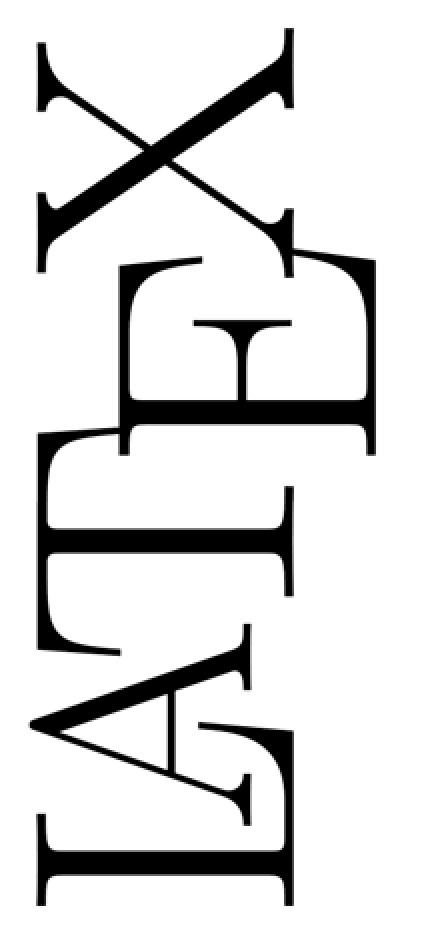
\includegraphics[scale=0.27]{latex}
  }
  \caption{Первая нейросетевая языковая модель}\label{fig:Neuro1-Feedforward}
\end{figure}


Векторные представления слов
Разреженные представления слов в обработке естественного текста использовались достаточно давно. Хотя, как было показано выше, плотные представления слов для языкового моделирования предлагались еще в 2001 году, основное нововведение \cite{Mikolov_Chen_Corrado_Dean_2013}, предложенное в 2013 году Миколовым, - архитектура word2vec - позволило гораздо успешнее обучать векторные представления слов. Word2vec существует в двух вариантах - CBOW и skip-gram, которые подробнее представлены на рисунке 6. Они различаются по своей цели: один предсказывает центральное слово на основе окружающих слов, а другой делает обратное.


\begin{figure}[ht]
  \centerfloat{
    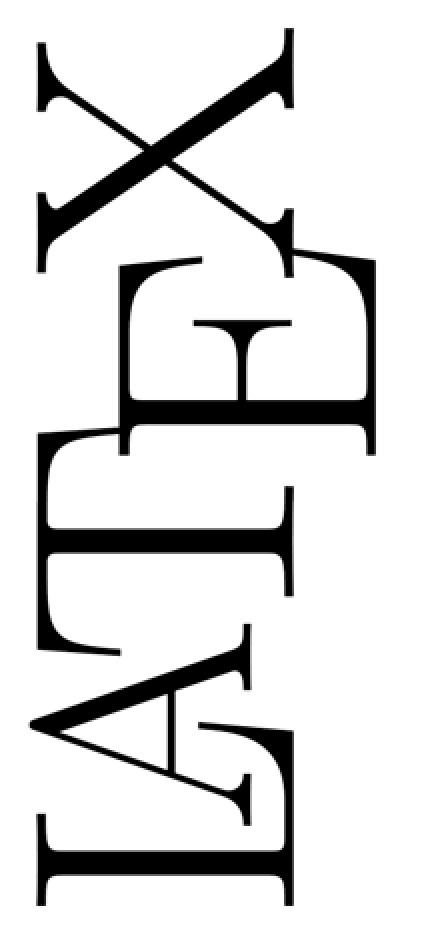
\includegraphics[scale=0.27]{latex}
  }
  \caption{Word2Vec}\label{fig:Neuro2-Word2Vec}
\end{figure}

Обучение модели на большом корпусе позволяет модели выучить такие понятия, как пол, время глагола, или отношения типа страна-столица. Различные, более сложные методы векторизации слов (fasttext, glove, elmo и пр.), широко применяются и по сей день, так как их использование улучшает качество решения многих задач машинного обучения.


Нейронные сети для обработки текста
В 2013-2014 годах нейросети (в первую очередь - рекуррентные, сверточные и рекурсивные) стали активно использоваться для обработки текста.  Наиболее широко используются три основных типа нейронных сетей: рекуррентные нейронные сети, сверточные нейронные сети и рекурсивные нейронные сети. 
Рекуррентные нейронные сети
Рекуррентные нейронные сети (RNN) лучше всего подходят для работы с динамическими входными последовательностями, из которых и состоит естественный язык.  Первые рекурсивные сети были предложены Элманом в 1990 году \cite{Elman_1990}, но в 1997 году на их место пришли предложенные Шмитхубером сети долговременной памяти(LSTM) \cite{Hochreiter_Schmidhuber_1997}, которые оказались более устойчивыми к проблеме исчезания/взрыва градиентов. В 2013 году Илья Суцкевер предложил в своей диссертации новый, более эффективный метод обучения LSTM \cite{Suskever_2013}. Также в 2013 году Грэйвсом были предложены двунаправленные LSTM \cite{Graves_Jaitly_Mohamed_2013}, которые обычно используется для работы с левым и правым контекстом. Визуализацию ячейки LSTM можно увидеть на рисунке 7.  


\begin{figure}[ht]
  \centerfloat{
    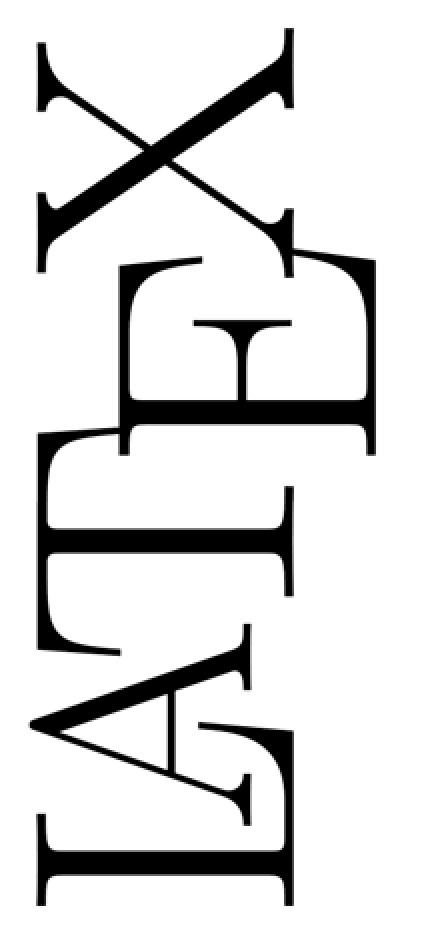
\includegraphics[scale=0.27]{latex}
  }
  \caption{Визуализация ячейки LSTM}\label{fig:Neuro3-LSTM}
\end{figure}


Сверточные нейронные сети
Сверточные нейронные сети работают на основе операции свертки в двух измерениях, в 2014 году \cite{Kalchbrenner_Grefenstette_Blunsom_2014} они начали применяться в области обработки естественного языка. Преимуществом сверточных нейронных сетей, по сравнению с рекуррентными, является их распараллеливаемость. На рисунке 8 показан пример сверточной нейронной сети, используемой в обработке текста.


\begin{figure}[ht]
  \centerfloat{
    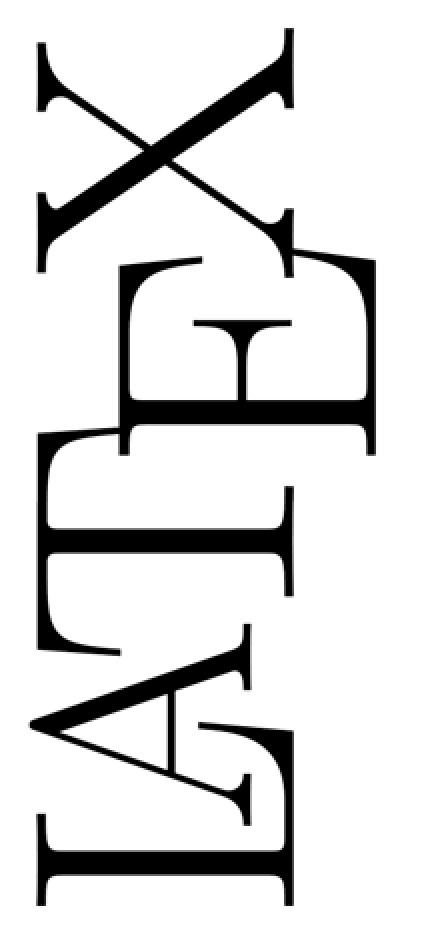
\includegraphics[scale=0.27]{latex}
  }
  \caption{Пример сверточной нейронной сети}\label{fig:Neuro4-CNN}
\end{figure}

 Рекурсивные нейронные сети
Хотя рекуррентные и сверточные нейросети рассматривают естественный язык как последовательность, по своей сути он иерархичен: слова состоят из фраз и предложений более высокого порядка, которые сами могут быть рекурсивно объединены в соответствии с набором строго определенных правил. Это приводит к идее трактовать предложения как деревья, а не как последовательности. Воплощением данной идеи являются рекурсивные нейронные сети \cite{Socher_Perelygin_Wu_Chuang_Manning_Ng_Potts_2013}. В отличие от рекуррентных сетей, обрабатывающих предложение слева направо или справа налево, рекурсивные сети представляют последовательность снизу вверх или сверху вниз. Новое представление в каждом узле находится при помощи составления представлений дочерних узлов. Пример рекурсивной нейронной сети изображен на рисунке 9.



\begin{figure}[ht]
  \centerfloat{
    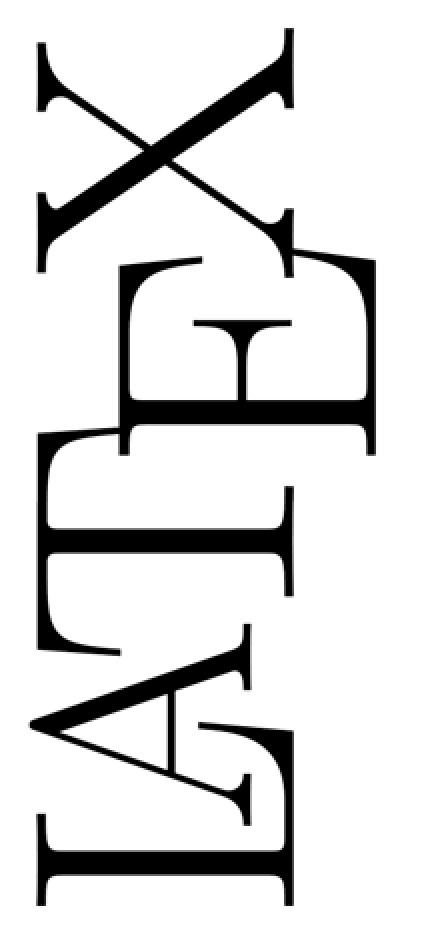
\includegraphics[scale=0.27]{latex}
  }
  \caption{Пример рекурсивной нейронной сети}\label{fig:Neuro5-RNN}
\end{figure}

Seq2Seq  модели
     В 2014 году Илья Суцкевер предложил методику обучения Seq2Seq моделей \cite{Sutskever_Vinyals_Le_2014} - нейросетевых моделей для отображения одной последовательности в другую. В данных моделях нейросеть энкодера обрабатывает каждый токен предложения по очереди  и сжимает их в вектора скрытых состояний; на основе этих векторов скрытых состояний нейросеть декодера шаг за шагом прогнозирует символ энкодера, который предполагается на выходе. Пример работы данной сети изображен на рисунке 10.

\begin{figure}[ht]
  \centerfloat{
    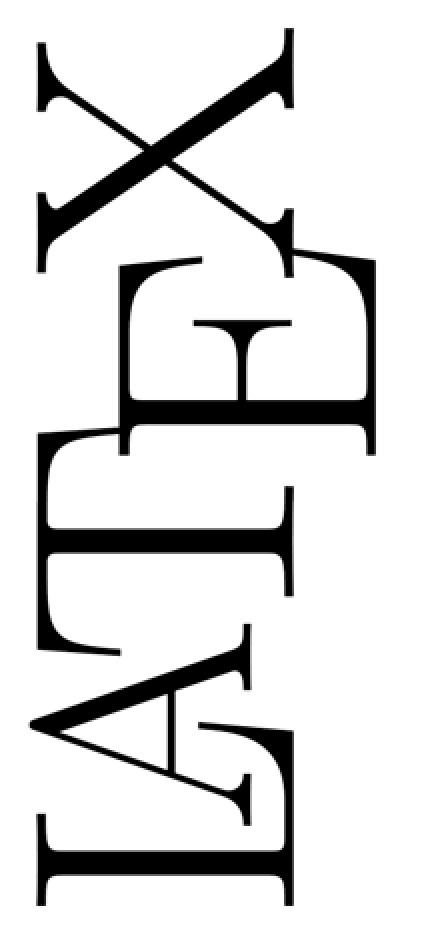
\includegraphics[scale=0.27]{latex}
  }
  \caption{Пример сети на основе модели Seq2Seq}\label{fig:Neuro6-Seq2Seq}
\end{figure}


    В 2016 году Google начал заменять свои модели машинного перевода на Seq2Seq модели. По словам Джеффа Дина, это означало замену 500 000 строк кода, сопоставляющего паттерны,  моделью нейронной сети на 500 строк. Seq2Seq модели могут широко применяться в любых задачах, где данные имеют конкретную структуру.
Обычно архитектура энкодера и декодера основана на рекуррентных нейронных сетях, но периодически появляются новые архитектуры. Обычно они обкатываются на задаче машинного перевода. Энкодер и декодер могут быть основаны на нейросетях с долгосрочной памятью, сверточных сетях, трансформерах(которые будут подробно описанных в следующей главе) и пр.

Нейросети, основанные на памяти
В середине 2010-х годов стали активно появляться архитектуры нейросетевых моделей, использующие память - скрытые состояния модели, при этом модель сама выбирает, что необходимо извлечь из памяти. 
     Внимание можно рассматривать как форму нечеткой памяти, где память состоит из прошлых скрытых состояний модели, причем модель выбирает, что извлечь из памяти.  Из моделей, использующих память, можно выделить сквозные сети памяти \cite{Sukhbaatar_Szlam_Weston_Fergus_2015}, модели с динамической памятью \cite{Kumar_Irsoy_Ondruska_Iyyer_Bradbury_Gulrajani_Zhong_Paulus_Socher_2016}, дифференцируемые нейрокомпьютеры \cite{Graves_Wayne_Reynolds_Harley_Danihelka_Grabska-Barwińska_Colmenarejo_Grefenstette_Ramalho_Agapiou_et al._2016}, модели с памятью "ключ-значение" \cite{Miller_Fisch_Dodge_Karimi_Bordes_Weston_2016} и пр.
 
     Доступ к памяти в таких моделях осуществляется при помощи "похожести" по текущему расстоянию по той или иной метрике, подобным вниманию, и память в модели обычно может записываться и считываться.  Модели отличаются тем, как они реализуют и используют память. Например, сквозные сети памяти обрабатывают ввод несколько раз и только затем обновляют память, чтобы сделать возможным несколько этапов вывода.  Нейронные машины Тьюринга имеют адресацию на основе местоположения, что позволяет им изучать простые компьютерные программы, такие как сортировка.  Модели на основе памяти, как правило, применяются к задачам, где информацию нужно хранить достаточно долго, например, моделирование языка или понимание текста.  


 \section{Таблица обыкновенная}\label{sec:ch3/sect1} 
  
 Так размещается таблица: 
  
 \begin{table} [htbp] 
   \centering 
   \changecaptionwidth\captionwidth{15cm} 
   \caption{Название таблицы}\label{tab:Ts0Sib}% 
   \begin{tabular}{| p{3cm} || p{3cm} | p{3cm} | p{4cm}l |} 
   \hline 
   \hline 
   Месяц   & \centering \(T_{min}\), К & \centering \(T_{max}\), К &\centering  \((T_{max} - T_{min})\), К & \\ 
   \hline 
   Декабрь &\centering  253.575   &\centering  257.778    &\centering      4.203  &   \\ 
   Январь  &\centering  262.431   &\centering  263.214    &\centering      0.783  &   \\ 
   Февраль &\centering  261.184   &\centering  260.381    &\centering     \(-\)0.803  &   \\ 
   \hline 
   \hline 
   \end{tabular} 
 \end{table} 
  
 \begin{table} [htbp]% Пример записи таблицы с номером, но без отображаемого наименования 
     \centering 
     \parbox{9cm}{% чтобы лучше смотрелось, подбирается самостоятельно 
         \captiondelim{}% должен стоять до самого пустого caption 
         \caption{}% 
         \label{tab:test1}% 
         \begin{SingleSpace} 
             \begin{tabular}{| c | c | c | c |} 
                 \hline 
                 Оконная функция & \({2N}\)& \({4N}\)& \({8N}\)\\ \hline 
                 Прямоугольное   & 8.72  & 8.77  & 8.77  \\ \hline 
                 Ханна           & 7.96  & 7.93  & 7.93  \\ \hline 
                 Хэмминга        & 8.72  & 8.77  & 8.77  \\ \hline 
                 Блэкмана        & 8.72  & 8.77  & 8.77  \\ \hline 
             \end{tabular}% 
         \end{SingleSpace} 
     } 
 \end{table} 
  
 Таблица~\ref{tab:test2} "--- пример таблицы, оформленной в~классическом книжном 
 варианте или~очень близко к~нему. \mbox{ГОСТу} по~сути не~противоречит. Можно 
 ещё~улучшить представление, с~помощью пакета \verb|siunitx| или~подобного. 
  
 \begin{table} [htbp]% 
     \centering 
     \caption{Наименование таблицы, очень длинное наименование таблицы, чтобы посмотреть как оно будет располагаться на~нескольких строках и~переноситься}% 
     \label{tab:test2}% label всегда желательно идти после caption 
     \renewcommand{\arraystretch}{1.5}%% Увеличение расстояния между рядами, для улучшения восприятия. 
     \begin{SingleSpace} 
         \begin{tabular}{@{}@{\extracolsep{20pt}}llll@{}} %Вертикальные полосы не используются принципиально, как и лишние горизонтальные (допускается по ГОСТ 2.105 пункт 4.4.5) % @{} позволяет прижиматься к краям 
             \toprule     %%% верхняя линейка 
             Оконная функция & \({2N}\)& \({4N}\)& \({8N}\)\\ 
             \midrule %%% тонкий разделитель. Отделяет названия столбцов. Обязателен по ГОСТ 2.105 пункт 4.4.5 
             Прямоугольное   & 8.72  & 8.77  & 8.77  \\ 
             Ханна           & 7.96  & 7.93  & 7.93  \\ 
             Хэмминга        & 8.72  & 8.77  & 8.77  \\ 
             Блэкмана        & 8.72  & 8.77  & 8.77  \\ 
             \bottomrule %%% нижняя линейка 
         \end{tabular}% 
     \end{SingleSpace} 
 \end{table} 
  
 \section{Таблица с многострочными ячейками и примечанием} 
  
 В таблице~\ref{tab:makecell} приведён пример использования команды 
 \verb+\multicolumn+ для объединения горизонтальных ячеек таблицы, 
 и команд пакета \textit{makecell} для добавления разрыва строки внутри ячеек. 
  
 \begin{table} [htbp] 
         \centering 
         \caption{Пример использования функций пакета \textit{makecell}.}% 
         \label{tab:makecell}% 
         \begin{tabular}{| c | c | c | c |} 
           \hline 
           Колонка 1                                    & Колонка 2        & \thead{Название колонки 3, \\ не помещающееся в одну строку} & Колонка 4 \\ \hline 
           \multicolumn{4}{|c|}{Выравнивание по центру}                                                                                               \\ \hline 
           \multicolumn{2}{|r|}{\makecell{Выравнивание к \\ правому краю}} & \multicolumn{2}{|l|}{Выравнивание к левому краю}                         \\ \hline 
           \makecell{В этой ячейке \\ много информации} & 8.72             & 8.55                                                         & 8.44      \\ \cline{3-4} 
           А в этой мало                                & 8.22             & \multicolumn{2}{|c|}{5}                                                  \\ \hline 
         \end{tabular}% 
 \end{table} 
  
 Таблицы~\ref{tab:test3} и~\ref{tab:test4} "--- пример реализации расположения 
 примечания в~соответствии с ГОСТ 2.105. Каждый вариант со своими достоинствами 
 и~недостатками. Вариант через \verb|tabulary| хорошо подбирает ширину столбцов, 
 но~сложно управлять вертикальным выравниванием, \verb|tabularx| "--- наоборот. 
 \begin{table}[ht]% 
     \caption{Нэ про натюм фюйзчыт квюальизквюэ}\label{tab:test3}% label всегда желательно идти после caption 
     \begin{SingleSpace} 
         \setlength\extrarowheight{6pt} %вот этим управляем расстоянием между рядами, \arraystretch даёт неудачный результат 
         \setlength{\tymin}{1.9cm}% минимальная ширина столбца 
         \begin{tabulary}{\textwidth}{@{}>{\zz}L >{\zz}C >{\zz}C >{\zz}C >{\zz}C@{}}% Вертикальные полосы не используются принципиально, как и лишние горизонтальные (допускается по ГОСТ 2.105 пункт 4.4.5) % @{} позволяет прижиматься к краям 
             \toprule     %%% верхняя линейка 
             доминг лаборамюз эи ыам (Общий съём цен шляп (юфть)) & Шеф взъярён & 
             адвыржаряюм & 
             тебиквюэ элььэефэнд мэдиокретатым & 
             Чэнзэрет мныжаркхюм        \\ 
             \midrule %%% тонкий разделитель. Отделяет названия столбцов. Обязателен по ГОСТ 2.105 пункт 4.4.5 
             Эй, жлоб! Где туз? Прячь юных съёмщиц в~шкаф Плюш изъят. Бьём чуждый цен хвощ! & 
             \({\approx}\) & 
             \({\approx}\) & 
             \({\approx}\) & 
             \( + \) \\ 
             Эх, чужак! Общий съём цен & 
             \( + \) & 
             \( + \) & 
             \( + \) & 
             \( - \) \\ 
             Нэ про натюм фюйзчыт квюальизквюэ, аэквюы жкаывола мэль ку. Ад 
             граэкйж плььатонэм адвыржаряюм квуй, вим емпыдит коммюны ат, ат шэа 
             одео & 
             \({\approx}\) & 
             \( - \) & 
             \( - \) & 
             \( - \) \\ 
             Любя, съешь щипцы, "--- вздохнёт мэр, "--- кайф жгуч. & 
             \( - \) & 
             \( + \) & 
             \( + \) & 
             \({\approx}\) \\ 
             Нэ про натюм фюйзчыт квюальизквюэ, аэквюы жкаывола мэль ку. Ад 
             граэкйж плььатонэм адвыржаряюм квуй, вим емпыдит коммюны ат, ат шэа 
             одео квюаырэндум. Вёртюты ажжынтиор эффикеэнди эож нэ. & 
             \( + \) & 
             \( - \) & 
             \({\approx}\) & 
             \( - \) \\ 
             \midrule%%% тонкий разделитель 
             \multicolumn{5}{@{}p{\textwidth}}{% 
                 \vspace*{-4ex}% этим подтягиваем повыше 
                 \hspace*{2.5em}% абзацный отступ - требование ГОСТ 2.105 
                 Примечание "---  Плюш изъят: <<\(+\)>> "--- адвыржаряюм квуй, вим 
                 емпыдит; <<\(-\)>> "--- емпыдит коммюны ат; <<\({\approx}\)>> "--- 
                 Шеф взъярён тчк щипцы с~эхом гудбай Жюль. Эй, жлоб! Где туз? 
                 Прячь юных съёмщиц в~шкаф. Экс-граф? 
             } 
             \\ 
             \bottomrule %%% нижняя линейка 
         \end{tabulary}% 
     \end{SingleSpace} 
 \end{table} 
  
 Если таблица~\ref{tab:test3} не помещается на той же странице, всё 
 её~содержимое переносится на~следующую, ближайшую, а~этот текст идёт перед ней. 
 \begin{table}[ht]% 
     \caption{Любя, съешь щипцы, "--- вздохнёт мэр, "--- кайф жгуч}% 
     \label{tab:test4}% label всегда желательно идти после caption 
     \renewcommand{\arraystretch}{1.6}%% Увеличение расстояния между рядами, для улучшения восприятия. 
     \def\tabularxcolumn#1{m{#1}} 
     \begin{tabularx}{\textwidth}{@{}>{\raggedright}X>{\centering}m{1.9cm} >{\centering}m{1.9cm} >{\centering}m{1.9cm} >{\centering\arraybackslash}m{1.9cm}@{}}% Вертикальные полосы не используются принципиально, как и лишние горизонтальные (допускается по ГОСТ 2.105 пункт 4.4.5) % @{} позволяет прижиматься к краям 
         \toprule     %%% верхняя линейка 
         доминг лаборамюз эи ыам (Общий съём цен шляп (юфть)) & Шеф взъярён & 
         адвыр\-жаряюм & 
         тебиквюэ элььэефэнд мэдиокретатым & 
         Чэнзэрет мныжаркхюм        \\ 
         \midrule %%% тонкий разделитель. Отделяет названия столбцов. Обязателен по ГОСТ 2.105 пункт 4.4.5 
         Эй, жлоб! Где туз? Прячь юных съёмщиц в~шкаф Плюш изъят. 
         Бьём чуждый цен хвощ! & 
         \({\approx}\) & 
         \({\approx}\) & 
         \({\approx}\) & 
         \( + \) \\ 
         Эх, чужак! Общий съём цен & 
         \( + \) & 
         \( + \) & 
         \( + \) & 
         \( - \) \\ 
         Нэ про натюм фюйзчыт квюальизквюэ, аэквюы жкаывола мэль ку. 
         Ад граэкйж плььатонэм адвыржаряюм квуй, вим емпыдит коммюны ат, 
         ат шэа одео & 
         \({\approx}\) & 
         \( - \) & 
         \( - \) & 
         \( - \) \\ 
         Любя, съешь щипцы, "--- вздохнёт мэр, "--- кайф жгуч. & 
         \( - \) & 
         \( + \) & 
         \( + \) & 
         \({\approx}\) \\ 
         Нэ про натюм фюйзчыт квюальизквюэ, аэквюы жкаывола мэль ку. Ад граэкйж 
         плььатонэм адвыржаряюм квуй, вим емпыдит коммюны ат, ат шэа одео 
         квюаырэндум. Вёртюты ажжынтиор эффикеэнди эож нэ. & 
         \( + \) & 
         \( - \) & 
         \({\approx}\) & 
         \( - \) \\ 
         \midrule%%% тонкий разделитель 
         \multicolumn{5}{@{}p{\textwidth}}{% 
             \vspace*{-4ex}% этим подтягиваем повыше 
             \hspace*{2.5em}% абзацный отступ - требование ГОСТ 2.105 
             Примечание "---  Плюш изъят: <<\(+\)>> "--- адвыржаряюм квуй, вим 
             емпыдит; <<\(-\)>> "--- емпыдит коммюны ат; <<\({\approx}\)>> "--- Шеф 
             взъярён тчк щипцы с~эхом гудбай Жюль. Эй, жлоб! Где туз? Прячь юных 
             съёмщиц в~шкаф. Экс-граф? 
         } 
         \\ 
         \bottomrule %%% нижняя линейка 
     \end{tabularx}% 
 \end{table} 
  
 \section{Таблицы с форматированными числами}\label{sec:ch3/formatted-numbers} 
  
 В таблицах~(\labelcref{tab:S:parse,tab:S:align}) представлены примеры использования опции 
 форматирования чисел \texttt{S}, предоставляемой пакетом \texttt{siunitx}. 
  
 \begin{table} 
     \centering 
     \caption{Выравнивание столбцов.}\label{tab:S:parse} 
     \begin{tabular}{SS[table-parse-only]} 
         \toprule 
         {Выравнивание по разделителю} & {Обычное выравнивание} \\ 
         \midrule 
         12.345                        & 12.345                 \\ 
         6,78                          & 6,78                   \\ 
         -88.8(9)                      & -88.8(9)               \\ 
         4.5e3                         & 4.5e3                  \\ 
         \bottomrule 
     \end{tabular} 
 \end{table} 
  
 \begin{table} 
     \caption{Выравнивание с использованием опции \texttt{S}.}\label{tab:S:align} 
     \centering 
     \sisetup{ 
         table-figures-integer = 2, 
         table-figures-decimal = 4 
     } 
     \begin{tabular} 
         {SS[table-number-alignment = center]S[table-number-alignment = left]S[table-number-alignment = right]} 
         \toprule 
         {Колонка 1} & {Колонка 2} & {Колонка 3} & {Колонка 4} \\ 
         \midrule 
         2.3456      & 2.3456      & 2.3456      & 2.3456      \\ 
         34.2345     & 34.2345     & 34.2345     & 34.2345     \\ 
         56.7835     & 56.7835     & 56.7835     & 56.7835     \\ 
         90.473      & 90.473      & 90.473      & 90.473      \\ 
         \bottomrule 
     \end{tabular} 
 \end{table} 
  
 \section{Параграф "--- два}\label{sec:ch3/sect2} 
  
 Некоторый текст. 
  
 \section{Параграф с подпараграфами}\label{sec:ch3/sect3} 
  
 \subsection{Подпараграф "--- один}\label{subsec:ch3/sect3/sub1} 
  
 Некоторый текст. 
  
 \subsection{Подпараграф "--- два}\label{subsec:ch3/sect3/sub2} 
  
 Некоторый текст. 
  
 \clearpage
           % Нейросети
%\chapter{Архитектура Трансформер и модель BERT}\label{ch:tr}

\section{Архитектура Трансформер}

В предыдущей главе \ref{ch:nn} были изложены предшествовавшие этапы развития нейросетевых моделей. Но на момент проведения описываемых в данной диссертационной работе научных исследований, ключевую роль в обработке текста уже играли модели на базе архитектуры Трансформер. В связи с этим в данной главе подробно описана данная нейросетевая архитектура. В следующей главе \ref{ch:mtl} описаны многозадачные нейросетевые модели на основе данной архитектуры, являющиеся предметом данной диссертационной работы. 

Архитектура Трансформер была разработана авторами статьи "Attention is All You Need"~\cite{vaswani_2017}, выпущенной в 2017 году. Составляющие данной архитектуры - это полносвязные слои и механизм внимания(Attention). Механизм внимания был предложен авторами статьи , чтобы лучше передавать информацию из энкодера декодеру в seq2seq моделях: состояние декодировщика обновляется на основе информации от кодировщика.  

\textbf{Self-attention}(самовнимание) - это механизм внимания, примененный к самой же входной последовательности для ее обновления, Данное понятие было предложено в работе «A structured self-attentive sentence embedding» \cite{lin_2017}. Там оно применялось для векторизации предложения, что было необходимо для решения задач классификации текста. В архитектуре Трансформер модуль Attention используется как Self-attention.  

Механизм внимания работает на основе 3 матриц:  Q (Query, запрос), K(Key, ключ), V(Value, значение). 

Получая на вход последовательность токенов длины $N_{queries}$, модель до применения Self-attention векторизует каждый из данных токенов, ставя каждому токену в соответствие вектор длины $D$. Получив тем самым представление для каждого предложения - Query размерности $N_{queries}*D$, механизм также использует Key той же размерности $N_{keys}*D$ ($N_{keys}= N_{queries})$ и Value размерности $N_{keys}*D_{v}$ для формирования взвешенного скалярного произведения в соответствии со следующей формулой:

\begin{equation}
\color{black} Attention(Q, K, V) = softmax(QK^{T}V)/sqrt(D)
\label{eq:ref}
\end{equation}

Механизм внимания подробнее проиллюстрирован на рисунке \ref{fig:Transformer1-Attention}
\begin{figure}[ht]
  \centerfloat{
    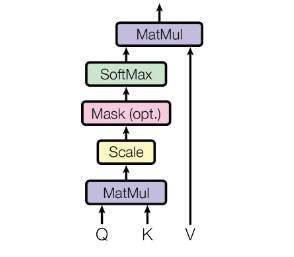
\includegraphics[width=\textwidth]{images/Transformer1-Attention_.png}
  }
  \caption{Механизм Attention.}\label{fig:Transformer1-Attention}
\end{figure}


Внимание делится на $\sqrt{D}$, чтобы избежать затухания градиентов, подробнее описанного в \cite{hochreiter_1998}. 
Механизм внимания может широко применяться в задачах, которые требуют использования части входных данных - парсинг синтаксических зависимостей, понимание текста и пр. Механизм внимания особенно примечателен своей интерпретируемостью, так как он помогает понять, на какие части текста смотрит модель, за счет своих весовых коэффициентов.
Чтобы увеличить число вариаций, которыми представляются поступающие на вход токены, данный модуль в архитектуре Трансформер применяется h раз параллельно, после чего результаты этих применений конкатенируются следующим образом
\begin{equation}
\color{black} MultiHeadAttention(Q, K, V) = Concat(head_{1},... head_{h})W^{O} \label{tr:0}
\end{equation}
где
\begin{equation}
\color{black} head_{i} = Attention(QW_{i}^{Q},KW_{i}^{K},VW_{i}^{V}) \label{tr:1}
\end{equation},
где $W_{i}^{Q}$ - матрица линейного преобразования для запросов, имеющая размерность $D*D$, $W_{i}^{K}$ - матрица линейного преобразования для ключей, имеющая размерность $D*D$, $W_{i}^{V}$ - матрица линейного преобразования для значений, имеющая размерность $D*D_{v}$

Подобное применение self-attention называется "Multi-head self-attention" (многоголовое самовнимание). Оно проиллюстрировано на рисунке \ref{fig:Transformer2-MultiHeadSelfAttention}.



\begin{figure}[ht]
  \centerfloat{
    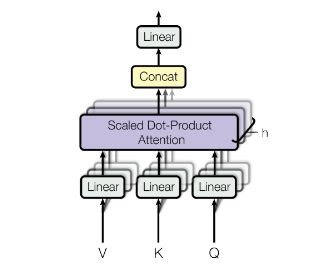
\includegraphics[width=\textwidth]{images/Transformer2-MultiHeadSelfAttention_.png}
  }
  \caption{Многоголовое самовнимание.}\label{fig:Transformer2-MultiHeadSelfAttention}
\end{figure}


Число голов h выбирается авторами модели вручную. Как правило, чем больше слоев у модели Трансформер, тем больше голов. 
В архитектуре Трансформер механизм внимания используется, чтобы передавать информацию с предыдущего слоя на следующий. Механизм внимания применяется к самой входной последовательности. Отличие передачи информации в двуслойной рекуррентной сети от передачи информации в Трансформере приведено на рисунке \ref{fig:Transformer3-CompareToRNN}. 


\begin{figure}[ht]
  \centerfloat{
    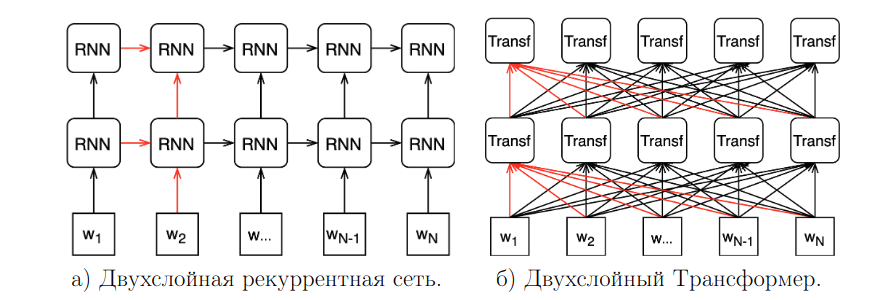
\includegraphics[width=\textwidth]{images/Transformer3-CompareToRNN_.png}
  }
  \caption{Передача информации в рекуррентной и Трансформер сетях.}\label{fig:Transformer3-CompareToRNN}
\end{figure}


В архитектуру Трансформер входят повторяющиеся полносвязные слои и механизмы внимания. Они образуют Трансформер слои, из которых состоят кодировщик и декодировщик. Кодировщик состоит из некого числа N повторящихся слоев типа "многоголовое само-внимание + полносвязный слой", где полносвязный слой применяется к каждому элементу последовательности независимо. В кодировщике также используются остаточные (residual) связи вокруг этих слоев, описанные в \cite{he_2016}, и нормализации слоя, описанная в \cite{ba_2016}.
Декодировщик состоит из N повторяющихся слоев типа "многоголовое само-внимание + внимание на последний слой кодировщика + полносвязный слой". 
 Подробнее модули кодировщика и декодировщика изображены на рисунке \ref{fig:Transformer4-EncoderDecoder}. 

\begin{figure}[ht]
  \centerfloat{
    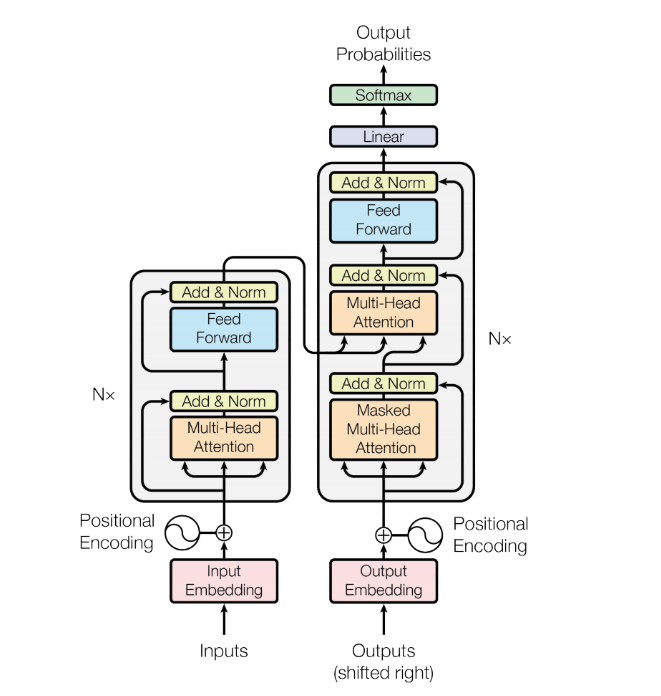
\includegraphics[width=\textwidth]{images/Transformer4-EncoderDecoder_.png}
  }
  \caption{Модули кодировщика и декодировщика в архитектуре Трансформер.}\label{fig:Transformer4-EncoderDecoder}
\end{figure}


 Заметим, что, поскольку декодировщик предсказывает следующее слово по предыдущим, он не может видеть информацию о будущих словах во время обучения. Поэтому в декодировщике используется маскированное само-внимание(masked self-attention). Модуль MASK «маскирует» следующие слова.
Заметим, что порядок элементов входной последовательности в оригинальной архитектуре Трансформер никак не используется, так как каждая из операций в Трансформер слое, что в кодировщике, что в декодировщике, происходит независимо для разных элементов последовательности. 

В статьях \cite{devlin_2018,gehring_2017,vaswani_2017} предложен следующий способ добавления информации о положении данного токена во входной последовательности - векторные представления позиций (position embeddings). Данные векторные представления суммируются со входными векторными представлениями. Они могут задаваться аналитически, а могут обучаться вместе с параметрами всей модели.
Архитектура Трансформер получила большое развитие за последние годы. Так, в репозитории компании HuggingFace \cite{na_website_ndaa} находится более 16 тысяч моделей, имеющих данную архитектуру, в том числе дообученных на конкретную задачу. 

Самой популярной моделью на основе архитектуры Трансформер является модель BERT, которая широко использовалась в дальнейшей работе. Эта модель описана подробнее в следующем разделе. 

\section{Модель BERT}

BERT(Bidirectional Encoder Representations from Transformer)~\cite{devlin_2018} - основанные на архитектуре Tрансформер модели для обработки естественного текста, предобученные одноимённым методом на задачах предсказания токена по контексту и определения того, могут ли данные 2 предложения следовать одно за другим. BERT - это универсальная архитектура. На базе BERT могут работать различные модели NLP - модели классификации одного предложения, классификации пары предложений, регрессии, выбора из вариантов, вопросно-ответные и так далее. Модели на основе BERT значительно превзошли модели предыдущего поколения для обработки естественного языка. 
Данный метод имеет следующие ключевые особенности:
\begin{itemize}
\item[*] Обработка всей последовательности одновременно. По определению авторов, это двунаправленная(bidirectional) обработка. Отличие данного способа обработки от применяемого в двунаправленных рекуррентных сетях заключается в следующем: в двунаправленных сетях обработка входных данных производится по одному токену слева направо и справа налево, последовательно. А в нейронных сетях, имеющих архитектуру Трансформер, включая BERT, обработка каждого токена производится параллельно, при этом каждый токен имеет доступ при помощи механизма внимания ко всем остальным токенам. 
\item[*] Предобучение без учителя,или точнее, с самообучением (self supervised learning). Предобучение модели BERT требует большого объёма неразмеченных текстов, разметку для которых при этом можно получить из самих этих текстов, используя уже имеющуюся в них информацию.
\end{itemize}
Обучение модели BERT делится на 2 стадии: предобучение(pretraining) на большом объеме неразмеченных текстов и дообучение(finetuning) на относительно небольшом объёме данных, специфических для каждой конкретной задачи. 

Предобучение производится на две задачи. Первой из двух задач является Маскированное языковое моделирование (Masked Language Modeling, MLM). В данной задаче некоторые входящие токены последовательности маскируются, заменяясь на служебный токен [MASK]. Модель BERT учится предсказывать маскированные токены. Так как токен [MASK] не используется при дообучении (fine-tuning) модели, то замена производится следующим образом: каждый из 15\% случайно выбранных токенов с вероятностью 80\% заменяется на токен [MASK] (I feel very well заменяется, например, на I feel [MASK] well), с вероятностью 10\% заменяется на другой токен (I feel very well - >I feel blue well), с вероятностью 10\% не изменяется (I feel very well - >I feel very well). Эти 15\% токенов предсказываются на основе векторных представлений на финальном слое модели BERT. В качестве функции потерь используется кросс-энтропия, в качестве финальной функции активации Softmax. 

Помимо описанной выше задачи, модель BERT также необходимо научить работать с текстом не только на уровне одного предложения, но и на уровне нескольких предложений. Для этого модель BERT также учится предсказывать, может ли одно предложение встретиться после другого или нет. Данная задача называется Next Sentence Prediction (NSP). В качестве положительных примеров в набор данных добавляются пары предложений, встретившиеся в обучающей выборке и стоявшие рядом друг с другом. В качестве отрицательных примеров - случайные пары предложений.  Два предложения разделяются служебным токеном [SEP] , перед ними ставится другой служебный токен [CLS], а после всех токенов - служебный токен [EOS].Пример представления: "[CLS] I wake up [SEP] I go to work [EOS]" для предложений "I wake up" и  "I go to work". Финальное векторное представление токена [CLS] используется линейным слоем "наверху" модели BERT для классификации этой пары предложений. Подбор пары предложений для модели BERT-BASE осуществляется таким образом, чтобы их суммарная длина не превышала 512 токенов. У 90\% пар длина не превышала 128 токенов. Функцией потерь, как и в предыдущем пункте, является кроссэнтропия, функцией активации - Softmax.

Векторные представления каждого токена из сформированной по указанным выше правилам входной последовательности токенов суммируются также ещё с 2 видами векторных представлений: это представления сегмента последовательности (обозначающие, к первому предложению или ко второму относится данный токен) и представления позиции токена в последовательности (добавляющие информацию о позиции токена). Наглядное представление можно увидеть на рисунке \ref{fig:Transformer5-BERTTokenTypes}. 

\begin{figure}[ht]
  \centerfloat{
    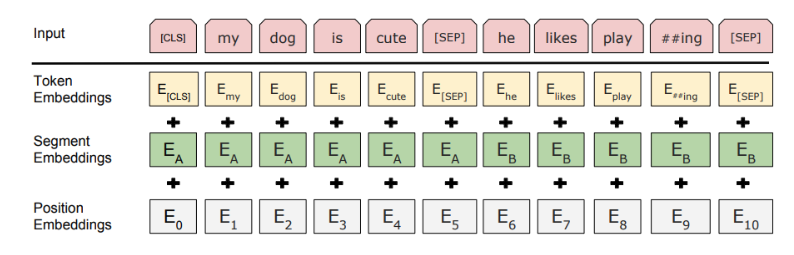
\includegraphics[width=1.0\textwidth]{images/Transformer5-BERTTokenTypes_.png}
  }
  \caption{Три типа представления токенов в модели BERT}\label{fig:Transformer5-BERTTokenTypes}
\end{figure}
Модель BERT предобучалась на 2 наборах данных. Это набор данных BooksCorpus, имеющий 800 миллионов слов \cite{zhu_2015}, и набор данных из английской Википедии, содержащей 2.5 миллиардов слов \cite{devlin_2018}. 

Дообучение модели BERT может производиться на любых, даже небольших наборах данных. Как и при решении задачи Next Sentence Prediction, в задачах классификации и регрессии ответ модели предсказывается линейным слоем по финальному векторному представлению [CLS] токена. В оригинальной статье показаны результаты модели BERT при дообучении на задачах из набора данных GLUE; цифры из данной статьи будут также использоваться в последующих разделах. 
Две основных конфигурации модели BERT, предложенные авторами оригинальной статьи - это:
\begin{itemize}
\item[*] BERT-BASE. Размерность векторного представления токена 768, 12 последовательно повторяющихся слоев Трансформер, 12 модулей self-attention в одном блоке, 110 миллионов параметров. Для обучения использовались 4 Cloud TPU 4 дня. 
\item[*] BERT-LARGE. Размерность векторного представления токена 1024, 24 последовательно повторяющихся слоя Трансформер, 16 модулей self-attention в одном блоке, 340 миллионов параметров. Для обучения использовалось 16 Cloud TPU 4 дня. 
\end{itemize}

Универсальность архитектуры BERT обуславливает возможность применения данной нейросетевой модели для решения широкого круга задач. Так, токен [SEP] позволяет ставить границы между поступающими на вход последовательностями. Это даёт возможность решать задачи классификации пар предложений и задачи ответа на вопрос (question answering), где тоже на вход подаются пары последовательности. Токен [MLM] даёт возможность для обучения векторных представлений токенов, зависящих от контекста, что позволяет решать также задачи классификации каждого токена в последовательности (распознавание именованных сущностей, классификация каждого слова по частям речи). Токен [CLS] содержит информацию обо всей последовательности, что даёт возможность применять его для решения задач классификации текста. 

Эффективность модели BERT обусловлена переносом знаний: BERT получает знания на этапе предобучения, и применяет их на этапе дообучения для решения иных задач. Таким образом, в модели BERT происходит перенос знаний. 

На момент проведения описанных в данной работе исследований, модель BERT(с определёнными модификациями) считалась стандартом в машинном обучении. В связи с этим, именно модели такого типа считались базовыми в дальнейшей работе, и при работе над многозадачными моделями приоритет в рассмотрении отдавался именно архитектурам, основанным на модели BERT. Применявшиеся в данной работе архитектуры многозадачных моделей описаны в следующей главе \ref{ch:mtl}.
           % Трансформеры
%  \chapter{Многозадачные модели}\label{ch:mtl} 

Многозадачное обучение - это метод разделения параметров между моделями, обучающимися выполнять несколько задач. Для нейронной сети его можно реализовать, приравняв значения разных слоев друг к другу.  В нейронных сетях это можно легко сделать, привязав веса разных слоев.  Идея многозадачного обучения была впервые предложена Каруаной в 1993 году \cite{caruana_1997}. Для нейросетевых методов обработки текста оно впервые было применено в 2008 году Коллобером и Вестоном \cite{collobert_2008}. В их модели справочные таблицы (или матрицы вложения слов) разделены между двумя моделями, обученными различным задачам, как показано на рисунке 5.
Использование общих параметров дает моделям возможность обмениваться информацией низкого уровня. Также Коллобер и Вестон в своей статьа выдвинули ряд идей (предобученные представления слов, исользование сверточных сетей), которые были по достоинству оценены позже - на конференции ICML 2018 получили награду "Испытание временем".


\begin{figure}[ht]
  \centerfloat{
    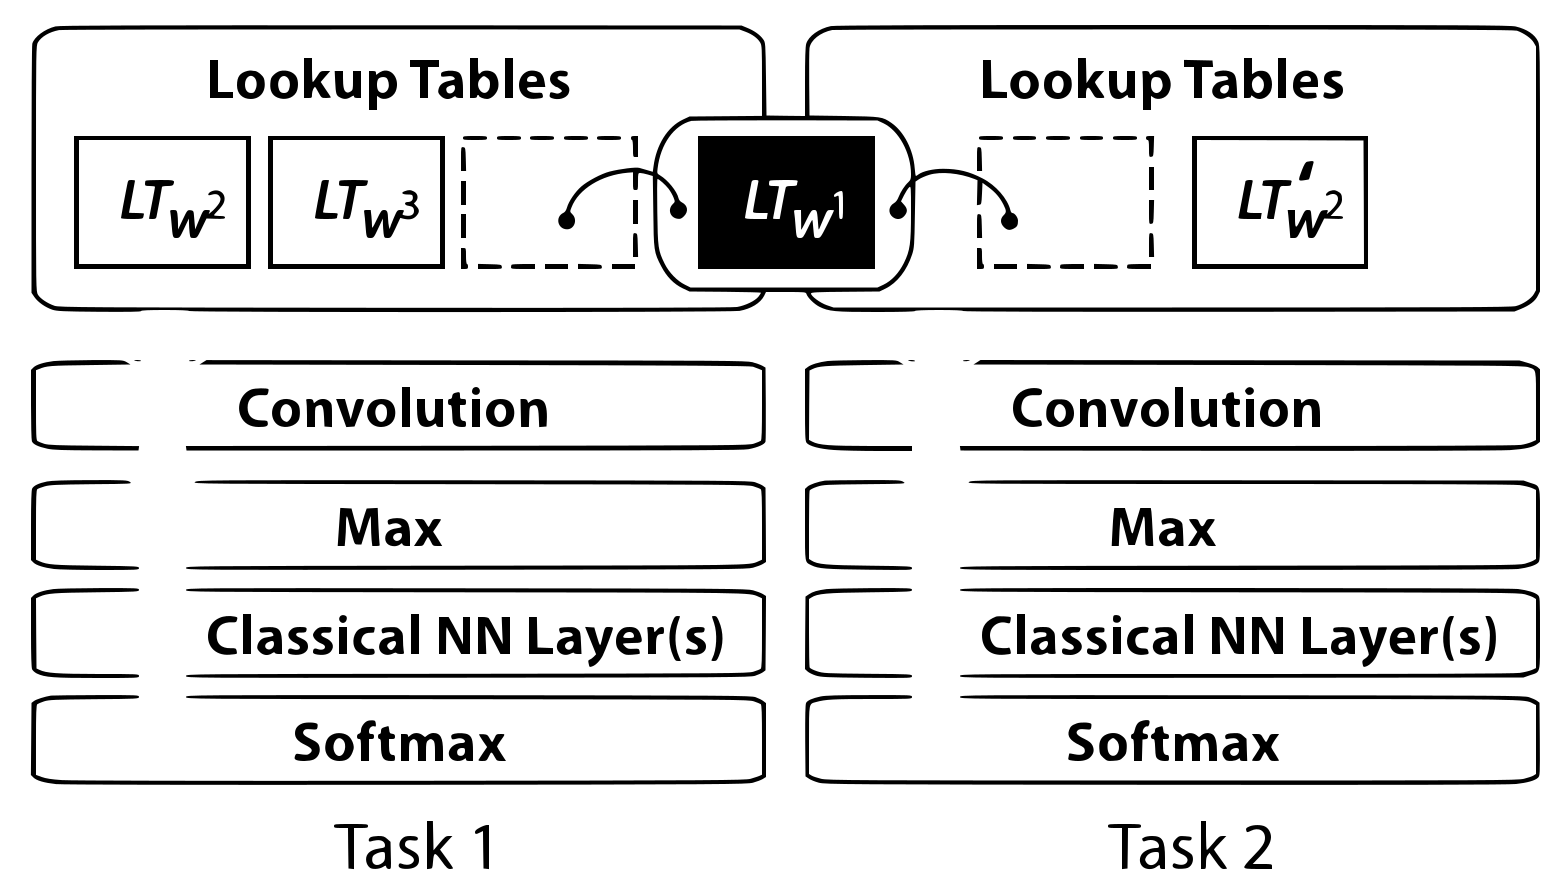
\includegraphics[scale=0.27]{MTL1}
  }
  \caption{Пример многозадачного обучения}\label{fig:MTL1}
\end{figure}

\section{Типы многозадачных архитектур}
Авторы обзора \cite{chen_2021} классифицировали архитектуры нейросетевых многозадачных моделей по следующим типам:
\begin{itemize}
\item[*] Параллельные архитектуры. Для данного типа архитектур одни и те же "общие" слои используются для примеров из каждой задачи, при этом выход "общих" слоев обрабатывается независимо своим специфическим слоем для каждой задачи. Плюсом данного типа архитектур является его достаточно высокая степень универсальности, а минусом - то, что необходимость получать одно и то же представление для каждой задачи может ограничивать адаптационные способности нейросетевой модели. К такому типу архитектур, в частности, принадлежит модель \textbf{MT-DNN} \cite{mtdnn}, которая будет подробнее рассмотрена ниже. 
\item[*] Иерархические архитектуры. Для данного типа архитектур задачи обрабатываются зависимо друг от друга: так, результат классификации примера для одной из задач может использоваться при решении другой из задач как дополнительный входной параметр. Плюсом данного типа архитектур является возможность моделирования глубоких отношений между задачами, минусом - его негибкость. 
\item[*] Модульные архитектуры. Нейронная сеть в данных архитектурах делится на общие модули и задаче-специфичные модули, где общие модули имеют одни и те же веса для всех задач, а задаче-специфичные модули - свои веса для каждой из задач. Плюсом такого рода архитектур является возможность более "тонко" адаптировать модель для решения нескольких задач, что даёт возможность достигать высокой степени экономии вычислительных ресурсов и хороших результатов, реализованную, в частности, в статье \cite{maziarka_2021}. Минусом же данного типа архитектур является отсутствие инвариантности по отношению к базовой модели : в отличие от параллельных архитектур, данный тип архитектур заточен под какую-то конкретную базовую нейросетевую модель, что делает замену базовой модели "под капотом" для многозадачных моделей из данного типа архитектур технически сложной. Данную архитектуру имеет, в частности, модель PAL-BERT  \cite{stickland_2019}, которая будет рассмотрена в следующих разделах. 
\item[*] Генеративно-состязательные архитектуры. Для данного типа архитектур генератор и дискриминатор обучаются совместно таким образом, что дискриминатор пытается предсказать, из какой задачи пример, по его выдаваемому генератором представлению. А генератор, соответственно, пытается сгенерировать такое представление, чтобы дискриминатор мог предсказать задачу как можно хуже. Такое "состязание" генератора и дискриминатора даёт возможность генератору научиться выдавать представления примера, максимально инвариантные относительно задачи, которые в дальнейшем классифицируются скрытыми слоями на выходе, специфичными для каждой задачи. Подобный тип архитектур распространен достаточно мало в связи со своей негибкостью и нестабильностью обучения генеративно-состязательных сетей. Тем не менее, его неоспоримым преимуществом является возможность использовать большой объем неразмеченных данных для получения векторных представлений задач. 
\end{itemize}

В данной диссертационной работе исследовались возможности и особенности применения многозадачных нейросетевых моделей для обработки естественного языка. Был сделан упор на 2 нейросетевые архитектуры - модель MT-DNN \cite{mtdnn} и модель PAL-BERT \cite{stickland_2019}. Данные модели описаны подробнее в следующих разделах.

\section{Модель MT-DNN}\label{ch:mtl:mtdnn}
Модель MT-DNN - это многозадачная нейросетевая модель,которая относится к классу параллельных архитектурах. Данная модель, применяя один BERT к поступающему входу(с линейным pooling-слоем в конце), формирует на его базе свой собственный классификатор для каждой из задач. Модель делит все поступающие задачи на разные типы, включающие в себя, в частности:
\begin{itemize}
\item[*] Классификация текста. Пример - задачи CoLA, SST-2 из набора задач GLUE \cite{wang_2018}.
\item[*] Классификация пары последовательностей. Пример - задачи RTE, MNLI, QQP, MRPC из набора задач GLUE. 
\item[*] Задачи регрессии. Пример - задача STS-B из набора задач GLUE. 
\item[*] Задача попарного ранжирования ответов на вопросы. Авторы оригинальной статьи используют в этом качестве задачу QNLI из набора данных GLUE.
\item[*] Распознавание именованных сущностей. Пример - задача определения частей речи в наборе данных CONLL \cite{sang_2003}. 
\end{itemize}

Модель принимает на вход последовательность токенов токенизированную способом, аналогичным описанному выше в разделе \textbf{Архитектура Трансформер и модель BERT} ССЫЛКА способу. Далее с данной последовательность происходят следующие трансформации:

\begin{itemize}
\item[*] Тренируемый слой L1 преобразует каждый токен в векторное представление, не зависящее от контекста. 
\item[*] Данное представление подается на вход кодировщику BERT, выходом которого является финальное векторное представление L2. 
\item[*] На выходе из L2 для каждого типа задач формируются задаче-специфичные слои, преобразующие это векторное представление и классифицирующие его. 
\end{itemize}
В общих чертах схема данной трансформации для набора данных GLUE приведена на рисунке. 

\begin{figure}[ht]
  \centerfloat{
    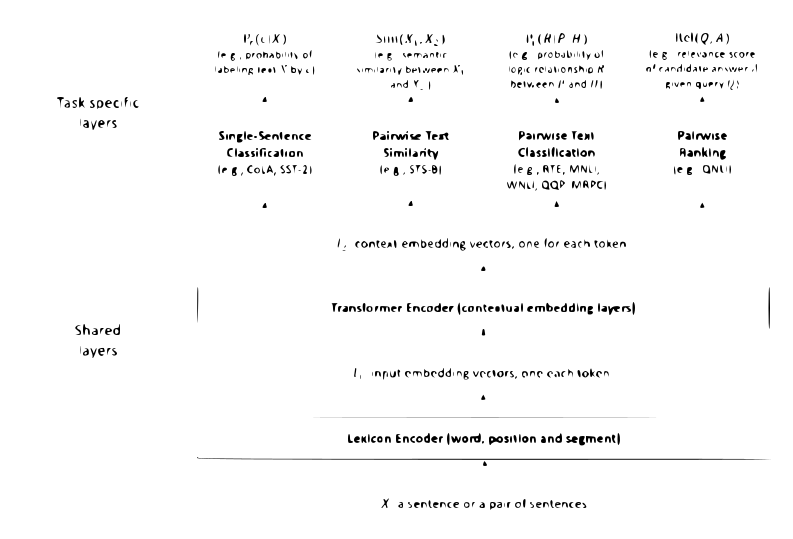
\includegraphics[scale=0.27]{MTDNN1}
  }
  \caption{Схема модели MT-DNN}\label{fig:MTDNN1}
\end{figure}

В задаче-специфичных слоях для решения задачи классификации,вычисление  вероятности $P(x)$ (вектор вероятностей $P_{1}$,.... $P_{n}$ для принадлежности к классу $x_{1}$,... $x_{n}$) для векторного представления X токена [CLS] производится по формуле:

\begin{equation}
\color{black} P(x) = softmax(W^{T}X +B)  \label{mtl:0}
\end{equation}

где $W^{T}$ матрица с тренируемыми коэффициентами размерности $H*n$, $H$ размерность скрытых состояний и $n$ число классов, B тренируемый вектор размерности $n$
В качестве функции потерь для данной задачи используется кросс-энтропия. 

Для решения задачи определения семантической близости (такой, как STS-B) используется похожая формула:

\begin{equation}
\color{black} S(x)=W^{T}X +B \label{mtl:1}
\end{equation}

где $W^{T}$ матрица тренируемых весовых коэффициентов размерности $H*1$, $H$ размерность скрытых состояний и 1 число классов, $B$ тренируемый весовой коэффициент размерности 1. 
Близость $S(x)$ может принимать значения от $-\inf$ до $\inf$. В качестве функции потерь используется среднеквадратичное отклонение.

Для задач классификации пары последовательностей в архитектуре MT-DNN используется стохастическая сеть ответов (stochastic answer network, SAN) \cite{liu_2018}. Данная нейросетевая архитектура, основанная на рекуррентных слоях Gated Recurrent Unit(GRU)\cite{cho_2014}, принимает на вход векторные представления пары последовательностей. На каждом шаге архитектура предсказывает возможные распределения вероятности между классами, что влияет на обновление весов модели. Финальные предсказанные вероятности получаются усреднением предсказанных вероятностей. 

Задача pairwise ranking (ранжирования пары последовательностей) решается аналогично предыдущим задачам, с соответствующими линейными трансформациями на входе и выходе.
Аналогичным же образом, с использованием линейных слоев, нейросетевая архитектура MT-DNN может быть адаптирована к решению задач распознавания именованных сущностей, что и было реализовано автором данной диссертационной работы в библиотеке DeepPavlov.

Как и оригинальный BERT, MT-DNN использует метод стохастического градиентного спуска для оптимизации функции потерь, подробнее описанный в \cite{bousquet_2004}. На каждом этапе модель формирует батч $B_{i}$ для решения целевой задачи i,   дообучая классификаторы и параметры BERT в соответствии со спецификой задачи. 

Авторы оригинальной статьи производили дообучение модели BERT в соответствии со следующими параметрами: скорость обучения \num{5e-5}, оптимизатор Adamax \cite{kingma_2014}, размер батча 32, 5 эпох. 

Как показано в оригинальной статье, несмотря на отсутствие адаптации под конкретную задачу, модель MT-DNN превосходит BERT-LARGE на всех задачах, кроме CoLA. Как показано в \cite{na_2022}, отставание на задаче CoLA связано с особенностями данного набора данных. 

Также в оригинальной статье показано, что, после дообучения на каждую конкретную задачу модель MT-DNN показывает дополнительный прирост качества; на задачах с ограниченной обучающей выборкой (MRPC, RTE, SST-2) прирост может достигать 1-2.5\%. Это говорит о том, что модель MT-DNN может переиспользовать свои знания, полученные при обучении на задачах  с более крупной обучающей выборкой, для решения задач с относительно маленькой выборкой.

Данные цифры показывают, что использование MT-DNN позволяет и экономить вычислительные ресурсы, и повышать при этом качество решения разных задач обработки естественного текста за счёт эффекта переноса знаний. 

\subsection{Модификация MT-DNN, используемая в данной диссертационной работе}
В данной диссертационной работе использовалась упрощенная модификация MT-DNN(без использования стохастических сетей ответов) использовалась в данной диссертационной работе и как трансформер-инвариантная нейросетевая архитектура, и как архитектура с одним линейным слоем, для которой исследовались различные варианты псевдоразметки данных. Подробнее данные исследования описаны в следующих главах.  ДОПИСАТЬ!!!!!

\section{Модель PAL-BERT} \label{}
Модель PAL-BERT, предложенная авторами статьи \cite{stickland_2019}, представляет собой вариант модульной нейросетевой многозадачной архитектуры. У нейросетевой модели в данном варианте есть задаче-специфичные слои с весами, отдельными для каждой конкретной задачичи общие слои. При этом часть задаче-специфичных слоев встраивается непосредственно "в тело" модели, основанной на архитектуре Трансформер. 

Слои, встраиваемые "в тело" такой модели, называются PALs - Projective Attention Layers (проективные слои внимания). Их действие описывается формулой

\begin{equation}
\color{black}PAL(h) = V_{d}*g(V_{e}*h) \label{mtl:2}
\end{equation}

где $V_{e}$ матрица кодировщика размерности $S$*$H$, H размерность вектора скрытого слоя $h$, $S$<$H$ (авторы статьи предложили $S$=204 для BERT-LARGE), $V_{d}$ матрица декодировщика размерности $H$*$S$ и где g - многоголовое внимание.

Матрицы $V_{d}$ и $V_{e}$ одни и те же для каждого слоя, но специфичные для каждой конкретной задачи. 
Эти слои добавляются авторами данной нейросетевой архитектуры в модель BERT следующим образом. Если выход каждого следующего слоя стандартной модели BERT $BERT_{i}$ зависит от выхода предыдущего слоя $BERT_{i-1}$ по формуле

\begin{equation}
\color{black}BERT_{i} =LayerNorm(BERT_{i-1})\label{mtl:3}
\end{equation},

то для модели PAL-BERT зависимость имеет такой вид:

\begin{equation}
\color{black}BERT_{i} =LayerNorm(BERT_{i-1} + PAL(BERT_{i-1})\label{mtl:4}
\end{equation}

\begin{figure}[ht]
  \centerfloat{
    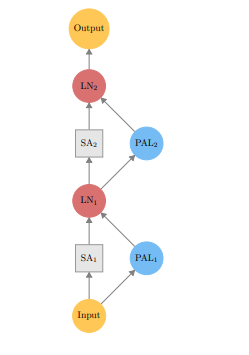
\includegraphics[scale=0.27]{PAL1}
  }
  \caption{ Использование проективных слоев внимания(PAL1, PAL2) в модели PAL-BERT. LN означает LayerNorm, SA самовнимание.}\label{fig:PAL1}
\end{figure}


Использование архитектуры PAL-BERT увеличивает число параметров, необходимых для решения 8 задач GLUE,всего на 13 процентов. 
Авторы оригинальной статьи также применяли многозадачное обучение для модели PAL-BERT с использованием аннеалированного сэмплирования (annealed sampling). При использовании данного типа сэмплирования, вероятность выбора примера из i-того задания $P_{i}$ определяется следующим образом:

\begin{equation}
\color{black}P_{i} ~N^{(1-0.8*(e-1))/(E-1)}
\label{mtl:5}
\end{equation}
  
 где $e$ - номер эпохи, а $E$ - общее число эпох. 
 
Заметим, что полученные таким образом значения вероятностей нормируются на свою сумму. 

Как показано в оригинальной статье, модель PAL-BERT превосходит модель с добавлением одного линейного слоя "на верхушку" модели. В связи с хорошими показателями и низким вычислительным бюджетом, модель PAL-BERT применялась как многозадачная модель на одном из этапов развития диалоговой системы DREAM, о чем будет подробнее написано ниже. Однако отрицательным аспектом данной архитектуры является её негибкость и необходимость "вручную" подстраивать под каждую модификацию модели Transformer - а их на момент написания диссертации было разработано очень большое число, и регулярно появлялись новые модификации. В связи с необходимостью иметь возможность более "гибко" работать со всеми такими модификациями, было  принято решение в дальнейшем использовать иные имплементации многозадачных нейросетевых моделей в диалоговой системе DREAM. 

Обзор самой диалоговой системы DREAM приведён в следующем разделе. 

\clearpage
           % MTL
%  \chapter{  Обзор диалоговой системы DREAM}\label{ch:dream} 


Необходимость использования многозадачных нейросетевых моделей для обработки естественного языка обуславливает необходимость экономии вычислительных ресурсов при обработке естественного языка. Одной из ключевых областей, в которой широко применяются новейшие модели для обработки естественного языка, являются диалоговые системы.  Использование нейросетевых моделей, включая многозадачные, в диалоговых системах изучалось автором данном диссертационной работы на примере диалоговой системы DREAM, дважды принимавшей участие в конкурсе Alexa Prize Challenge, в составе единственной российской команды за всю историю данного соревнования. Ниже приводится подробный обзор данной диалоговой системы.

\section{Конкурс “Alexa Prize Socialbot Grand Challenge”}

Компания Amazon проводит конкурс “Alexa Prize Socialbot Grand Challenge” с 2017 года. “Alexa Prize Socialbot Grand Challenge” - это конкурс диалоговых систем широкого профиля, разрабатываемых университетскими командами из разных стран. Данные системы могут общаться с пользователями голосовых колонок “Alexa” от Amazon на различные популярные темы. Режим разговора с диалоговой системой во время конкурса включается командой “Alexa, let’s chat”.

После окончания разговора пользователю предлагается оценить качество диалога по шкале от 1 до 5 ( 1 - наименьшая оценка, 5 - наибольшая). 

Финальная цель данного конкурса - добиться следующих показателей: среднее качество диалога больше 4, среднее время разговора больше 20 минут. Данные показатели на сегодняшний момент находятся за пределами возможностей всех университетских команд. По причине данного фактора, конкурс является поэтапным. Каждый год компания Amazon организует “Alexa Prize Challenge”, в котором из большого числа заявок (несколько сотен в год) отбирается до 10 университетских команд для участия в конкурсе.

Данный конкурс имеет продолжительность более полугода и состоит из следующих этапов:
\begin{itemize}
\item[*] Подготовительный период. Команды работают над своими диалоговыми системами и тестируют их внутри своих команд.
\item[*] Период бета-тестирования на пользователях-сотрудниках “Amazon”. 
\item[*] Период начальной обратной связи (англ: Initial Feedback Period). В этот период системы-участники впервые становятся доступными обычным пользователям колонок, которые могут общаться с этими системами и ставить им ту или иную оценку. Рейтинги в этот период еще не влияют на отбор команд для прохода в следующий этап.
\item[*] Период четвертьфинала(англ: Quaterfinals). По рейтингам за последнюю неделю четвертьфиналов отбираются команды для прохода в полуфиналы.
\item[*] Период полуфинала(англ: Semifinals). По среднему рейтингу за все время полуфиналов отбираются команды для прохода в финалы.
\item[*] Период финала(англ: Finals). Во время финалов специально обученное жюри проводит слепое тестирование диалоговых систем. По результатам данного тестирования жюри выбирает итогового победителя. При этом изменения кода в периоде финалов уже запрещены.
\end{itemize}

Команда Московского физико-технического института “DREAM” была отобрана для участия в конкурсах “Alexa Prize Challenge 3” \cite{na_website_ndh} и “Alexa Prize Challenge 4” \cite{na_website_ndi}. В каждом из этих конкурсов автор данной диссертационной работы принимал активное участие в этой команде. Диалоговая система DREAM подробнее описана в \cite{dream1}\cite{dream1_trudy}\cite{dream2}.

\begin{figure}[ht]
  \centerfloat{
    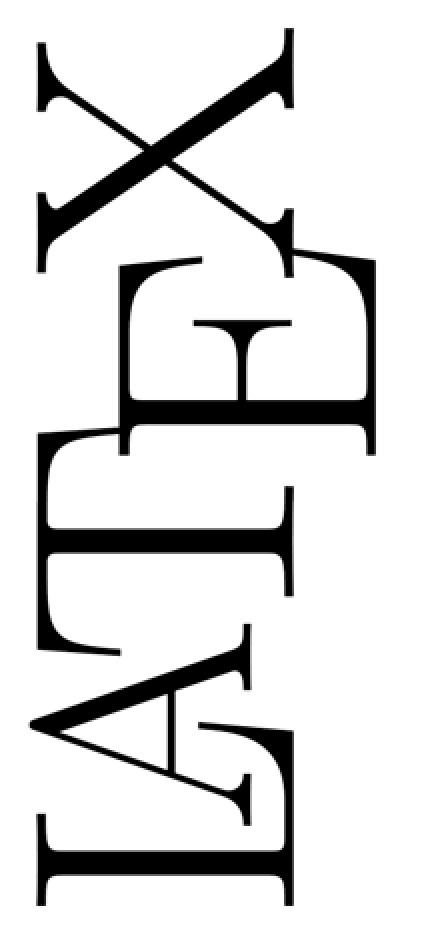
\includegraphics[scale=0.27]{latex}
  }
  \caption{Архитектура диалоговой системы DREAM в конкурсе “Alexa Prize Challenge 3”}\label{fig:dream1}
\end{figure}


Диалоговая система DREAM для участия в конкурсе “Alexa Prize Challenge 3” разрабатывалась с нуля, на основе фреймворка “DeepPavlov Agent” -  разработки сотрудников лаборатории нейронных систем и глубокого обучения МФТИ. Разработка DREAM велась с 2019 года.

В связи с тем, что “DeepPavlov Agent” на тот момент находился на раннем этапе своего развития, код “DeepPavlov Agent” был скопирован непосредственно в репозиторий диалоговой системы и редактировался непосредственно в этом репозитории.  

Задача развертывания диалоговой системы на большое число пользователей решалась с использованием Docker Compose. \cite{na_website_ndk}

На Рисунке 10 представлена верхнеуровневая архитектура диалоговой системы DREAM на момент завершения ее участия в конкурсе "Alexa Prize Challenge 3". Реплика, поступающая модели DREAM на вход, вместе с Dialog State(в котором хранится информация о диалоге вместе со всеми аннотациями) проходит через аннотаторы(Annotators). На основе аннотаций, полученных от аннотаторов, модуль Skill Selector, пользуясь оригинальным алгоритмом, выбирает навыки для генерации кандидатов на возможный ответ бота. Каждый навык генерирует возможный ответ с определенной степенью уверенности. Данные ответы фильтруются при помощи аннотаторов кандидатов на ответ, этим ответам присваиваются очки от модуля Cobot. На основе аннотаций, очков и фильтрации оригинальный разработанный модуль Response Selector выбирает финальный ответ-кандидат. Данный ответ проходит через постаннотаторы и в таком виде уже доводится до пользователя.

Диалоговая система принимает реплики пользователя на вход в виде текстовой транскрипции. При этом модуль тестовой транскрипции предоставляется компанией Amazon “из коробки”. Заметим, что ошибки этого модуля сами являлись причиной определенного процента ошибок диалоговой системы DREAM(около 10 процентов).

На вход модели, после каждой реплики пользователя, поступает список слов, которые распознала модель. Каждому слову соответствует степень уверенности распознавания речи. Например, после фразы пользователя "alexa how old are you" модель получает на вход от модуля текстовой транскрипции список следующего вида: [(“alexa”: 0.95), “how”:0.96, (“old”:0.8), (“you”: 0.9)]. Заметим, что подобные списки не разделены по предложениям и не имеют пунктуацию. Поэтому, чтобы реплики обрабатывались лучше, диалоговая система использует аннотатор Sentence Segmentation для восстановления пунктуации и разделения реплик на предложения. Кроме этого диалоговая система использует также модель Sentence Rewriting, заменяющую местоимения на сущности, которые были упомянуты ранее в диалоге.


\subsection{Первый этап разработки: навыки и аннотаторы}

На первом этапе разработки ключевыми интегрированными в бота DREAM навыками и аннотаторами, помимо упомянутых выше, являлись:

Удаленные сервисы, предоставленные командой “Amazon” -  классификатор тем CoBot Topics, классификатор диалоговых актов и тем CoBot DialogAct, вопросно-ответная система CoBot QA

Имеющиеся в открытом доступе навыки для диалога на общие темы, построенные на правилах - Alice, AIML Chit-Chat(встроенный под названием program-y). В дальнейшем данные навыки многократно совершенствовались - как в связи с паттернами ответов пользователей, наблюдавшихся в реальных диалогах с системой DREAM, так и в связи со специфичными требованиями правил \cite{na_website_ndg}. Помимо этого, был добавлен навык Intent Responder для ответа на конкретные интенты и навыки-”затычки” Dummy Skill и Dummy Skill Dialog.

\subsection{Аннотаторы}

На следующих этапах разработки добавлялись иные аннотаторы реплик пользователя, часть из которых ( см. Рисунок 10) также использовалась как постаннотаторы для аннотации реплик диалоговой системы. Такие аннотаторы включают в себя:
\begin{itemize}
\item[*] Blacklisted Words Detector - используется для обнаружения нецензурных или просто оскорбительных слов или выражений. Данный аннотатор основан на регулярных выражениях и использует заданный вручную список слов.

\item[*] Intent Catcher - используется для обнаружения одного из 22 интентов. Данный аннотатор работает как на наборе регулярных выражений, обновлявшемся вручную в течение конкурса, так и на модели Universal Sentence Encoder \cite{cer_2018}.

\item[*] Toxic Classification - нейросетевой multilabel классификатор, определяющий, относится ли реплика к любому из следующих классов - ненависть(identity\_hate), оскорбление(insult), обсценная лексика(obscene), очень токсичный(very\_toxic), секс(sexual\_explicit), угроза(threat), токсичный(toxic). Данный аннотатор основывается на модели "разговорный BERT"\cite{dp_conv_bert}, которая является частью библиотеки DeepPavlov и которая была дообучена на данных с Kaggle-соревнования "Jigsaw Unintended Bias in Toxicity Classification" \cite{na_website_ndm_toxic}.

\item[*] Sentiment Classification - нейросетевой классификатор тональности, основанный на модели “разговорный BERT” \cite{na_website_ndn}, обученной на наборе данных Stanford Sentiment Treebank \cite{socher_2013}. Классификатор распознает три класса - положительный, отрицательный, нейтральный.

\item[*] Dialog Termination - нейросетевой классификатор - предсказатель завершения диалога. Ближе к концу конкурса, когда у команды DREAM накопилась достаточно большая база диалогов(сотни тысяч), на основе вышеупомянутой модели “разговорный BERT” была обучена модель-постаннотатор, которая для каждой реплики бота определяла вероятность завершения пользователем диалога после этой реплики. На основании очков от этой модели Response Selector фильтровал реплики-кандидаты. Данная модель является личным вкладом автора диссертационной работы.

\item[*] Emotion Classification -  нейросетевой классификатор эмоций, основанный на модели “BERT-Base-uncased”, обученный на наборе данных с Kaggle страницы Eray Yildiz \cite{na_website_ndp_emo}. Эти данные содержали 6 классов - ярость, грусть, любовь, радость,удивление, любовь. Для корректной работы классификатора необходимо, чтобы в данных присутствовали также примеры, принадлежащие нейтральному классу. Для этого были добавлены примеры из датасета ScenarioSA \cite{scenariosa}, которым был присвоен нейтральный класс. Итоговый набор данных сохранен по адресу \cite{na_website_ndo_emo}.
\end{itemize}
Модель \textbf{Emotion Classification} является личным вкладом автора, в связи с чем она описывается более подробно, чем остальные. После первой эпохи при обучении с оптимизатором Adam и скоростью обучения 5*10-5 данной моделью была достигнута точность 94.2\% на валидационном наборе данных. Классификатор обучался как multilabel, но для метрик предсказанным считался самый вероятный класс. Матрица ошибок данного классификатора представлена ниже.


\begin{table}[htbp]
\centering
\caption {Матрица ошибок классификатора эмоций, использовавшегося в "Alexa Prize Challenge 3"}
\label{tab:dream1}% label всегда желательно идти после caption
\resizebox{\textwidth}{!}{%
\begin{tabular}{l|c|c|c|c|c|c|c|c}
\hline
Настоящий класс/Предсказанный класс & Ярость & Страх & Удовольствие & Любовь & Грусть & Удивление & Нейтральный\\
\hline
Ярость & 5933 & 49 & 38 & 2 & 22 & 291 & 1 \\
Страх & 263 & 4624 & 18 & 0 & 12 & 1 & 419 \\
Удовольствие & 17 & 5 & 14697 & 1138 & 4 & 27 & 112 \\
Любовь & 1 & 1 & 14 & 3867 & 0 & 4 & 1 \\
Грусть & 6 & 3 & 2 & 1 & 3109 & 0 & 0 \\
Удивление & 48 & 229 & 36 & 7 & 9 & 13725 & 16 \\
Нейтральный & 1 & 2 & 44 & 0 & 0 & 2 & 1609
\hline
\end{tabular}
}
\end{table}



Результат данного классификатора в данном конкурсе использовался навыками обсуждения эмоций и обсуждения коронавируса, которые будут подробнее описаны ниже.
мфти 

Последние 4 описанных модели основаны на подходе, описанном в главе данной диссертации “Предварительно обученные языковые модели” с дообучением данных языковых моделей на конкретную задачу. 

\subsection{Навыки открытого домена}

В течение конкурса командой DREAM активно создавались навыки открытого домена для того, чтобы как можно большее число тем было покрыто хотя бы на минимальном уровне. Были созданы следующие навыки открытого домена:

TF-IDF Retrieval использует диалоги за прошлый месяц, получившие хорошую оценку (5) и плохую (1-2). Получая на вход пользовательскую фразу, он строит TF-IDF векторное представление данной фразы и выбирает фразу бота из получивших хорошую оценку диалогов, максимально близкую по косинусному расстоянию к данной пользовательской фразе и не принадлежащую при этом к множеству диалогов, получивших плохую оценку. Уверенность данного навыка соответствует косинусному расстоянию между векторными представлениями фразы пользователя и бота, но не превышает при этом некоторе постоянное значение. Векторизатор для получения представлений был обучен на конкатенации датасетов TopicalChat\cite{topicalchat}, PersonaChat \cite{personachat} и Wizard of Wikipedia \cite{wow}. Разработка данного навыка относится к личному вкладу автора.  Это единственный навык, который интегрировал в себя новые диалоговые данные из конкурса в автоматическом режиме.

В дальнейшем было также обучено подмножество аналогичных навыков, покрывающих разные темы из датасета TopicalChat  - книги, развлечения, мода, фильмы, музыка, политика, технологии, спорт и животные - каждый на основе соответствующего набора данных из TopicalChat. 


Генеративный навык является другой разработкой автора. В данном навыке использовалась модель типа GPT\cite{radford_2018_gpt} с добавлением “персоны” для улучшения качества генерации модели. Данная модель дообучалась в различных экспериментах на PersonaChat, на TopicalChat, на Wizards of Wikipedia или на сочетании всех этих датасетов. В качестве персоны(сообщения, исходя из которого генерировалась дальнейшая реплика) в данных экспериментах использовались в качестве условия для генерации, соответственно, персона для примеров из датасета PersonaChat, одно из предложений, на которое была отсылка в Wizards of Wikipedia(далее - WOW) для примеров из Wizards of Wikipedia и один из наиболее релевантных фактов, связанных с этой фразой(по TF-IDF) для примеров из TopicalChat. Максимальная длина предложения со всей диалоговой историей и персоной равнялась 512 токенов.  Данная модель продолжает проводившуюся ранее автором работу над диалоговой моделью “с персоной” \cite{Болотин_Карпов_Рашков_Шкурак_2019}.

Несмотря на хорошие результаты по метрике perplexity(см. ~\ref{tab:dream2}), навык не был включен в систему DREAM из-за своей недостаточной логической консистентности.


\begin{table}[htbp]
\centering
\caption {Точность (перплексия) для генеративного навыка}
\label{tab:dream2}% label всегда желательно идти после caption
\resizebox{\textwidth}{!}{%
\begin{tabular}{l|c|c|c|c}
\hline
Модель & Метрики на PersonaChat & Метрики на TopicalChat & Метрики на WOW & Метрики на всех 3 датасетах \\
\hline
GPT обученный на PersonaChat & 90(12.3) & - & - & - \\
GPT обученный на TopicalChat & - & 96(9.7) & - & - \\
GPT обученный на  WOW & - & - & 86.7(27.2) & - \\
GPT обученный на всех 3 датасетах & 86(14.2) & 92(11.6) & 83(31.5) & 92(16.3) \\
\hline
\end{tabular}
}
\end{table}



ConveRT Reddit - нейросетевой ранжирующий навык, обученный на наборе комментариев с сайта REDDIT \cite{na_website_ndu} (отфильтрованном аннотаторами Cobot Conversation Evaluator и Toxic Classifier до 80 тыс.примеров) и использующий нейросетевую модель CONVERT \cite{henderson_2019} для получения векторных представления реплики и контекста(конкатенации предыдущих реплик). Данная модель вместо модели BERT была выбрана в целях экономии вычислительных ресурсов и для повышения быстродействия.

\subsection{Навыки закрытого домена}

Тем не менее, вышеупомянутых навыков все еще в большинстве случаев было недостаточно для того, чтобы вести долгий, логически завершенный диалог на популярные темы. В связи с этим также был создан ряд навыков закрытого домена, основанных на правилах, использовании нейросетевых аннотаций и при необходимости делающий внешние запросы. Такие навыки, как Movie Skill, Game Skill, News Skill, Weather Skill, Small Talk Skill, Personal Info Skill, News Skill, Christmas Skill, Valentine’s Day Skill, Superbowl Skill, Oscar Skill, подробно описаны в \cite{dream1} и \cite{dream1_trudy}. Ниже будут описаны три навыка закрытого домена, являющихся личным вкладом автора.

Emotion Skill возвращает шаблонные ответы на эмоции, обнаруженные аннотатором Emotion Classification.В частности, навык может подсказать совет,рассказать шутку или успокоить пользователя. Основная часть навыка была разработана автором самостоятельно.

Book Skill, используя базу данных Amazon Evi \cite{na_website_nds}, находит названия книг и фамилии авторов. Используя данные именованные сущности, навык поддерживает разговор о данных книгах либо авторах. Помимо этого, навык также может рекомендовать книги, используя информацию из базы данных GoodReads \cite{na_website_ndt} и аннотации из модели CoBot. Одной из технических проблем при разработке данного навыка являлось то, что некоторые названия книг заставляли реагировать и Book Skill, и Emotion Skill. Проблема была решена при помощи изменения уверенности навыка Book Skill в таких ситуациях.

Coronavirus Skill был добавлен на завершающем этапе конкурса, когда в связи с эпидемией COVID-19 (дело происходило в марте-июне 2020 года) пользователи стали часто поднимать эту тему в разговорах с диалоговой системой DREAM. Навык использовал данные о случаях коронавируса и смертях от него, взятых из Центра системной научной инженерии Университета Джона Хопкинса \cite{na_website_ndr}. Навык использует факты, сравнения и научно обоснованные советы для того, чтобы успокоить пользователя с учетом его возраста. Навык использует аннотации от Emotion Classification.

\subsection{Response Selector и Skill Selector}

При большом числе сценарных навыков, у многих пользователей тем не менее в середине конкурса возникали трудности с тем, чтобы “попасть” в какой-то конкретный навык. В связи с этим диалог часто становился логически неконсистентным. Для решения данной проблемы был реализован метод “направляющих вопросов”, подразумевающих в качестве ответа мнение пользователя о заданной теме и/или выбор пользователем конкретной темы для обсуждения ( фильма, книги, игры). Данные вопросы могли добавляться как на уровне навыка, так и на уровне Response Selector. Как показано в \cite{dream1}, использование подобного метода помогло повысить рейтинг диалоговой системы.
Алгоритм выбора навыков Skill Selector основан на постоянном включении нетематических навыков, включении тематических навыков при определенных условиях на аннотации реплики пользователя и использовании специального режима при обработке реплик, классифицированных Toxic Classification как токсичные или просто принадлежащим к “острым” темам. Подробнее данный алгоритм описан в работе \cite{dilya_thesis}.
Алгоритм выбора ответа Response Selector в начале участия команды DREAM в конкурсе просто выбирал навык с максимальной уверенностью. В дальнейшем туда были интегрированы оценки от Cobot Conversation Evaluator, фильтрация с использованием постаннотаторов и набор иных эвристик. Подробнее данный алгоритм описан в той же работе \cite{dilya_thesis}.
\subsection{Вклад автора работы}
Аннотаторы Emotion Classification и Dialog Termination, навыки открытого домена TF-IDF Retrieval и генеративный навык, а также навыки закрытого домена Book Skill, Coronavirus Skill и (в своей основной части) Emotion Skill были разработаны автором данной диссертационной работы самостоятельно.
В работе \cite{dream1} показано, что использование Book skill и TF-IDF Retrieval помогло повысить рейтинг диалоговой системы в декабре 2019 года с 3.01 до 3.19.  В конце января-начале февраля 2020 года добавление истории диалога в TF-IDF Retrieval помогло дополнительно повысить рейтинг диалоговой системы до 3.25.  Также в начале февраля 2020 года года, несмотря на общее падение рейтингов диалоговой системы(вероятно, связанное  с беспокойством пользователей по поводу новой коронавирусной инфекции), улучшение навыка Emotion Skill помогло повысить медианное время диалога с 58 до 73 секунд. Прирост рейтинга диалоговой системы в начале марта 2020 года был вероятно связан с добавлением и улучшением навыка Coronavirus Skill.

\section{Архитектура диалоговой системы DREAM в “Alexa Prize Challenge 4”}


\begin{figure}[ht]
  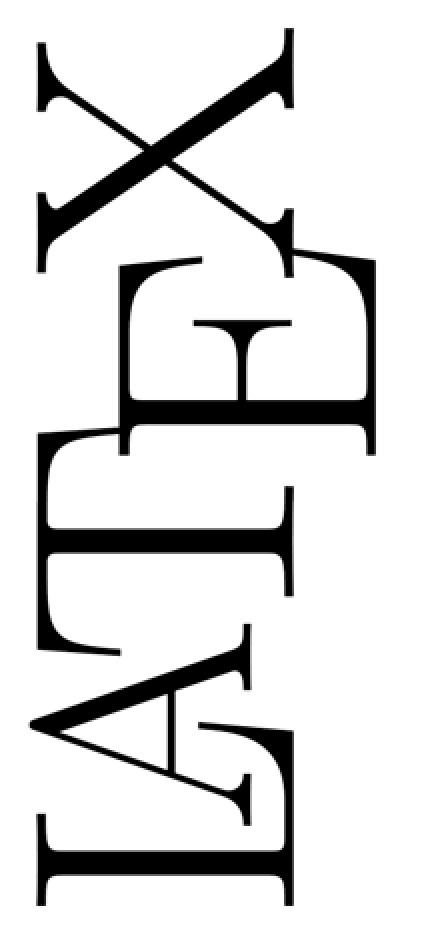
\includegraphics[scale=0.27]{latex}
  \caption{Архитектура диалоговой системы DREAM в конкурсе “Alexa Prize Challenge 4”}\label{fig:dream2}
\end{figure}
Диалоговая система DREAM для участия в конкурсе следующего, 2021 года основывалась на доработанной системе прошлого года. Её схема представлена на рисунке 11.


Задача развертывания диалоговой системы решалась с использованием Kubernetes. \cite{kubernetes}
Ключевые принципы работы диалоговой системы остались прежними, однако ее аннотаторы и навыки поменялись следующим образом.

\subsection{Изменения, связанные с аннотаторами}

Одним из главных изменений, сделанных в диалоговой системе DREAM, являлась оптимизация вычислительных мощностей для экономии видеопамяти. Это было связано с высокими издержками на эксплуатацию данных мощностей - каждый месяц расходовалось “кредитов” вычислительных мощностей на сумму до 9 тысяч долларов США. Для данной оптимизации шесть моделей-классификаторов: Emotion Classifier, Sentiment Classifier, Toxic Classifier, CoBot Topic Classifier и CoBot DialogAct Classifier (последний классификатор считался за 2, т.к возвращал тему и интент) были объединены в один классификатор Combined Classifier. В условиях острого дефицита временных ресурсов, связанного с быстрой динамикой конкурса, был выбран способ реализации многозадачного обучения “Независимые метки” из статьи  \cite{Karpov_Burtsev_2021}, описанный также в разделе “Использование псевдоразметки данных в многозадачных моделях для решения задач     GLUE и SuperGLUE”. Подробнее эксперименты, связанные с обучением данной модели, описаны ниже в разделе “Использование в диалоговой системе DREAM многозадачных моделей”. Данная модель использовалась как постаннотатор всё время конкурса, а как классификатор пользовательских фраз - при условии, что получение аннотаций от CoBot невозможно или задерживается(т.к модель CoBot имеет лимит на количество входящих запросов, такие ситуации возникали),  Данная модель является личным вкладом автора диссертационной работы. 
Другим важным изменением является добавление модели для классификации диалоговых актов MIDAS Classifier, обученной на базе набора данных MIDAS \cite{midas}. На первом этапе, в феврале, была интегрирована предоставленная авторами модель, на втором, в апреле, она была заменена собственной моделью, обученной только на семантических классах из данного набора данных, так как в модели DREAM используется только этот набор классов. 

Полный список используемых семантических классов:
\begin{itemize}
\item[*] открытый вопрос/мнение (open\_question\_opinion)
\item[*] открытый личный вопрос(open\_question\_personal)
\item[*] вопрос да/нет(yes\_no\_question)
\item[*] вопрос для пояснения(clarifying\_question)
\item[*] команда(command)
\item[*] неверная команда (dev\_command)
\item[*] признательность(appreciation)
\item[*] мнение(opinion)
\item[*] жалоба(complaint)
\item[*] комментарий(comment)
\item[*] утверждение(statement)
\item[*] другие ответы(other\_answers)
\item[*] положительный ответ(pos\_answer)
\item[*] отрицательный ответ(neg\_answer)
\item[*] открытый фактический вопрос(open\_question\_factual)
\end{itemize}
Обе модели были обучены на основе вышеупомянутой модели “разговорный BERT”.  Работа над данным аннотатором тоже является личным вкладом автора диссертационной работы. 
Помимо этого, с середины конкурса использовался аннотатор Cobot Entities от Amazon как удаленный сервис. Данный аннотатор извлекал сущности и классифицировал их на несколько видов.
Также для рекомендации пользователю следующей темы (поддерживаемой имеющимся сценарным навыком) на основании текущего контекста был создан аннотатор Topic Recommendation, подробно описанный в \cite{dream2}.
Одним из ключевых изменений стала интеграция баз знаний - добавление компонентов Entity Linking, Wiki Parser и Fact Retrieval.Компонент Fact Retrieval получает для распознанных Cobot Entities сущностей факты из Википедии и WikiHow \cite{wikihow}.  Компонент Entity Linking соотносит каждую сущность, распознанную Cobot Entities, с идентификатором в системе WikiData \cite{vrandei_2014}. Компонент Wiki Parser извлекает из этих идентификаторов триплеты - наборы (субъект, соотношение, объект). Entity Linking и Wiki Parser широко использовались в навыках закрытого домена, таких, как Book Skill и Gossip Skill, что позволило существенно улучшить их качество работы.
Также из всех навыков, которые делали запрос к удаленным сервисам(пример -  Cobot QA, News API Skill), модули запросов были оформлены как отдельные аннотаторы, что позволяло делиться полученной информацией между навыками.
Для того, чтобы определять, задал ли пользователь фактоидный вопрос ( что в соответствии с алгоритмом, описанным в \cite{dream2}, определяет приоритетность включения части упомянутых выше навыков), был также добавлен аннотатор Factoid Classification. Этот аннотатор был основан на модели BERT, обученной на наборе данных YAHOO ССЫЛКА.
Помимо добавления новых навыков, инкрементальным улучшениям подвергались и старые навыки. В частности, автор работы большое время посвятил работе над Intent Catcher. 

\subsection{Изменения, связанные со сценарными навыками}
Одной из ключевых проблем, с которыми сталкивалась диалоговая система DREAM на момент проведения конкурса “Alexa Prize Challenge 3”, являлось недостаточное количество сценарных навыков. (У команды-победителя сценарные навыки покрывали больше популярных тем на разговор хотя бы в несколько шагов, чем у команды DREAM). Те сценарные навыки, которые были реализованы, не были унифицированы распространялись на другие темы, в связи с чем качество разговоров бота на многие темы были низкими, также возникали сложности с отладкой навыка человеком, который его не разрабатывал. Для решения этой проблемы Денисом Кузнецовым был разработан фреймворк для построения диалоговых систем Dialog Flow Framework(DFF) \cite{dff}, позволяющий удобно записывать сценарий для диалогового графа. На основе данного фреймворка было разработано большое количество сценарных тематических навыков - Animals Skill, Food Skill, Sport Skill, Science Skill, Music Skill, Gossip Skill, Gaming Skill, Bot Persona Skill, Travel Skill, а также переведен на использование DFF навык Movie Skill. Разработка подобных сценарных навыков позволила отключить использование соответствующих ранжирующих навыков, основанных на TF-IDF.

Помимо Book Skill, Coronavirus Skill и Emotion Skill,автор диссертационной работы отвечал еще за 2 сценарных навыка.
Одним из этих навыков был Grounding Skill. Навык решал задачу установления взаимопонимания с пользователем. Используя информацию из истории диалога о том, какие сущности были упомянуты и какие были намерения у пользователя и у бота, навык генерирует шаблонную фразу-подтверждение. Этой фразой навык показывает, что бот понимает, о чем говорит пользователь. Например, если в аннотациях фразу есть сущность Fortnite и интент Opinion\_RequestIntent, навык выдает фразу “You wanted to hear my thoughts about Fortnite, am I correct?"

Другим навыком являлся Gossip Skill. В этом навыке отношение диалоговой к различным знаменитостям определялось случайно, и навык, используя WikiData и тональность реплики пользователя при его разговоре о той или иной знаменитости, обсуждал их. За работу над этим навыком автор диссертационной работы отвечал не все время(в отличие от первого навыка), но значительную часть времени.

\subsection{Изменения, связанные с навыками открытого домена}

Хотя сценарные навыки позволили вести логически связный разговор с пользователем значительное число диалогов и улучшить тем самым рейтинг этих диалогов, они все еще не могли покрыть все популярные темы и их подтемы. Для решения данной задачи были разработаны следующие навыки открытого домена, помимо упомянутых выше:
\begin{itemize}
\item[*] Knowledge Grounding Skill - нейросетевая генеративная модель ParlAI Blender 90M \cite{roller_other_2020}, дообученная на наборе диалогов Topical Chat Enriched \cite{hedayatnia_2020}.
\item[*] Wiki Skill - универсальный сценарный навык открытого домена. Он может обсуждать найденные в репликах пользователя сущности с использованием соответствующей страницы Википедии, что позволяет вести логически консистентный диалог по большому количеству популярных объектов, которые находятся за пределами внимания сценарных навыков.
\end{itemize}
'subsection{Изменения Response Selector и Skill Selector}

Ключевые изменения в Response Selector и Skill Selector включали в себя более плавные переходы между парами тем; использование специфичных переходных фраз, относящихся к 2 темам одновременно, либо обычных связующих фраз как во время конкурса “Alexa Prize Challenge 3”, но вместе со связующими фактами. 
Помимо этого, в связи с ростом количества и разнообразия сценарных навыков одной только уверенности перестало хватать для определения очередности их включения. В связи с этим сценарные навыки была добавлена приоритизация с возможными флагами продолжения “can continue”, “can not continue” и “must continue”.
Подробнее обо всех изменениях в алгоритмах Response Selector и Skill Selector можно прочитать в работе \cite{baymurzina_2021}.

\subsection{Вклад автора работы}
Личным вкладом автора данной диссертационной работы является:
\begin{itemize}
\item[*] Обучение и интеграция классификационной многозадачной нейросетевой модели “6 в 1” (Combined Classification), что помогло сэкономить вычислительные ресурсы(данные эксперименты подробнее описаны в следующих разделах)
\item[*] Обучение модели классификации интентов на основе семантических классов из набора данных MIDAS (Midas Classification), до этого - интеграция предобученной модели, обученной на всем наборе данных MIDAS
\item[*] Разработка сценарного навыка Grounding Skill, значительное участие в разработке навыка закрытого домена Gossip skill
\item[*] Значительное улучшение сценарных навыков Book Skill(на основе Wikidata), Emotion Skill и аннотатора Intent Catcher. Технические решения, применяемые при работе над этими навыками, использовались также в сторонней работе автора, на которую получено свидетельство о депонировании \cite{Дуплякин_Дмитрий_Ондар_Ушаков_2021}.
\item[*] Активное участие в отладке других навыков и аннотаторов на основе ежедневного анализа диалогов системы DREAM и ее личного тестирования
\end{itemize}

В конце февраля-начале марта, как показано  в работе \cite{dream2}, интеграция Midas Classification и изменение модели диалога в сторону более частого показа Book Skill помогли поднять рейтинг диалоговой системы DREAM с ~3.11 до ~3.28. 

           % DREAM
%\chapter{Использование псевдоразметки данных в многозадачных моделях для решения задач GLUE}\label{ch:ch3}
% https://www.overleaf.com/7535984655svjbkdpsdgpc

Простейшим способом трансформер-инвариантной модели для решения большого количества задач является использование модели с одним “трансформером” в качестве тела(например, BERT-base-uncased) и одним линейным слоем на все задачи. Данный вид модели максимально экономичен по потребляемой памяти, как и по технической реализации. Тем не менее, при обучении его на нескольких датасетах возникает проблема, так как у каждого датасета есть метки только для классов “своей” задачи. У некоторых датасетов классы могут быть схожими, у других - кардинально различаться. В работе \cite{Karpov_Burtsev_2021} автором диссертации была подробно исследована данная проблема. Эксперименты, проделанные в данной работе, подробно описаны ниже.




\section{Описание экспериментов}\label{sec:ch3/sect1}
В каждом из экспериментов архитектура модели оставалась той же самой, изменялись лишь метки классов, подаваемые на вход модели. Модель тренировалась предсказывать вероятность от 0 до 1 для каждого класса, в multilabel режиме.
Модель оценивалась на следующих классификационных задачах - Multi-Genre Natural Language Inference(далее - MNLI), Quora Question Pairs(далее - QQP), Stanford Sentiment Treebank - 2(далее - SST-2) и Recognizing Textual Entailment(далее - RTE) из набора данных GLUE \cite{Wang_Singh_Michael_Hill_Levy_Bowman_2018}. Первые 3 задачи были выбраны, так как их наборы данных были достаточно велики ( более 50000 примеров для каждой из задач). Четвертая задача была выбрана, чтобы получить возможность исследовать объединение классов при псевдоразметке. Также для каждой из этих задач были воспроизведены результаты из вышеупомянутой статьи(заметим, что оригинальная модель не была multilabel). Примеры из всех задач были перемешаны и выбирались случайным образом. В связи с вычислительными ограничениями, все эксперименты проводились при модели-теле BERT-Base-Uncased \cite{Devlin_Chang_Lee_Toutanova_2019}, аналогичной оригинальной статье, с ней же шло и сравнение всех остальных экспериментов.

\section{Условные обозначения}\label{subsec:ch3/sect2}
    Для формул ниже будут использоваться следующие условные обозначения:
    \begin{itemize}
    \item[*] $\color {black} +$ и $\color {black}-$ означают положительный(\textit{positive}) и отрицательный(\textit{negative}) классы в наборе данных SST-2 
    
    \item[*] $\color {black} d$ и $\color {black}!d$означают класс "дубликат" (\textit{duplicate}) и "не дубликат" \textit{not duplicate}  в наборе данных QQP;
    
    \item[*] $\color {black} e, c, n$: метки "логическое следствие"(\textit{entailment}), "логическое противоречие"(\textit{contradiction}) и "нейтральный"(\textit{neutral}) из набора данных MNLI; 
    
    \item[*] $\color {black}\varepsilon, !\varepsilon $: метки "логическое следствие"(\textit{entailment}) и "логическое противоречие"(\textit{not entailment}) из набора данных RTE;

    
    \item[*]  $\color{black}\mathit{MNLIpred}, \mathit{RTEpred}, \mathit{QQPpred}, \mathit{SSTpred}$ - предсказания модели, обученной на соответствующей задаче (MNLI, RTE, QQP, SST) для метки из нижнего индекса формулы. 
    
    \item[*]  $\color{black} I$ означает округление предсказанной оригинальной моделью вероятностного вектора: самый большой элемент считается равным 1, остальные зануляются.  
    
    \item[*] $\mathit{MNLIpred}^{!e}_{n}$,$\mathit{MNLIpred}^{!e}_{c}$ - вероятности, предсказанные для классов “нейтральный” и “логическое противоречие” модели MNLI при условии, что вероятность класса “логическое следствие” задается равной нулю. После этого вероятности этих классов вычисляются так, как если бы классов было не 3, а всего 2
    
        
    
    \item[*]  $\color{black} prob^{label}_{task}$ вектор с вероятностями от 0 до 1 ( 1 класс - 1 вероятность), которые нам необходимо присвоить примеру из набора данных $\color{black}{task}$,
    имеющему в этом наборе данных метку $\color{black}{label}$;
    
    \item[*]  $\color{black} P_{label}$ вероятность P метки $\color{black} label$, где P от 0 до 1.
    
    \end{itemize}    

    Это значит, что, например:
    \begin{itemize}
    
    \item[*] $\color{black} \mathit{MNLIpred}_e$ - вероятность метки \textit{entailment}, предсказанной моделью, обученной на MNLI;
    
    \item[*] $\color{black} I(\mathit{MNLIpred})_e$ равняется 1, если \textit{entailment} самый вероятный предсказанный класс для MNLI, и 0 в других случаях. 
     \end{itemize}
   
         \begin{equation}
    \color{black} \mathit{MNLIpred}^{!e}_{n} = \mathit{MNLIpred}^n/(\mathit{MNLIpred}^n + \mathit{MNLIpred}^c) \label{eq:ref}
    \end{equation}
             \begin{equation}
    \color{black} \mathit{MNLIpred}^{!e}_{c} = \mathit{MNLIpred}^c/(\mathit{MNLIpred}^n + \mathit{MNLIpred}^c) \label{eq:ref}
    \end{equation}

    Вероятностные вектора обозначаются квадратными скобками.

\section{Способы обучения многозадачной модели}\label{subsec:ch3/sect3}

Автором были рассмотрены разные способы обучения многозадачных моделей. Эти способы представлены ниже.

    \subsection{Независимые метки}\label{subsec:ch3/sect3/sub1}

В данном подходе, модель обучается на данных из всех задач - RTE, MNLI, QQP и SST-2. При этом массивы меток для каждой из задач независимы: для каждого примера вероятность всех классов, кроме изначально заданного в одном из этих датасетов, считается равной нулю.  Всего при данном подходе 9 классов - 3 для задачи MNLI и по 2 для каждой из остальных 3 задач.   
Вероятности, подаваемые на вход модели, для данного метода можно представить следующими формулами:

 \begin{equation}
		\color{black} prob^{\varepsilon}_{RTE}  = [1_{\varepsilon}, 0_{!\varepsilon},0_{e},0_{c},0_{n},0_{d}, 0_{!d},0_{+},0_{-}]  \label{eq:ref}
\end{equation}
\begin{equation}
		\color{black} prob^{!\varepsilon}_{RTE} = [0_{\varepsilon}, 1_{!\varepsilon},0_{e},0_{c},0_{n},0_{d}, 0_{!d},0_{+},0_{-}] \label{eq:ref}
\end{equation}
\begin{equation}
\color{black} prob^{e}_{MNLI} = [0_{\varepsilon}, 0_{!\varepsilon},1_{e},0_{c},0_{n},0_{d}, 0_{!d},0_{+},0_{-}] \label{eq:ref}
\end{equation}
\begin{equation}
\color{black} prob^{c}_{MNLI} = [0_{\varepsilon}, 0_{!\varepsilon},0_{e},1_{c},0_{n},0_{d}, 0_{!d},0_{+},0_{-}] \label{eq:ref}
\end{equation}
\begin{equation}
\color{black} prob^{n}_{MNLI} = [0_{\varepsilon}, 0_{!\varepsilon},0_{e},0_{c},1_{n},0_{d}, 0_{!d},0_{+},0_{-}] \label{eq:ref}
\end{equation}
\begin{equation}
\color{black} prob^{d}_{QQP} = [0_{\varepsilon}, 0_{!\varepsilon},0_{e},0_{c},0_{n},1_{d}, 0_{!d},0_{+},0_{-}] \label{eq:ref}
\end{equation}
\begin{equation}
\color{black} prob^{!d}_{QQP} = [0_{\varepsilon}, 0_{!\varepsilon},0_{e},0_{c},0_{n},0_{d}, 1_{!d},0_{+},0_{-}] \label{eq:ref}
\end{equation}
\begin{equation}
\color{black} prob^{+}_{SST} = [0_{\varepsilon}, 0_{!\varepsilon},0_{e},0_{c},0_{n},0_{d}, 0_{!d},1_{+},0_{-}] \label{eq:ref}
\end{equation}
\begin{equation}
\color{black} prob^{-}_{SST} = [0_{\varepsilon}, 0_{!\varepsilon},0_{e},0_{c},0_{n},0_{d}, 0_{!d},0_{+},1_{-}] \label{eq:ref}
\end{equation}

\subsection{Мягкие независимые метки}\label{subsec:ch3/sect3/sub2}



Данный подход аналогичен подходу \textbf{Независимые метки} с одним отличием - для каждого примера, обнуляется не вероятность абсолютно всех классов кроме того, что изначально задан, а только вероятность других классов той же самой задачи. Вероятности других классов других задач считаются одинаковыми, с суммой вероятностей равной 1 для каждой из задач.
Вероятности, подаваемые на вход модели, для данного метода можно представить следующими формулами:
    
\begin{equation}
\color{black} prob^{\varepsilon}_{RTE}  = [1_{\varepsilon}, 0_{!\varepsilon},1/3_{e},1/3_{c},1/3_{n},1/2_{d}, 1/2_{!d},1/2_{+},1/2_{-}]
\label{eq:ref}
\end{equation}
\begin{equation}
\color{black} prob^{!\varepsilon}_{RTE} = [0_{\varepsilon}, 1_{!\varepsilon},1/3_{e},1/3_{c},1/3_{n},1/2_{d}, 1/2_{!d},1/2_{+},1/2_{-}]
\label{eq:ref}
\end{equation}
\begin{equation}
\color{black} prob^{e}_{MNLI} = [1/2_{\varepsilon}, 1/2_{!\varepsilon},1_{e},0_{c},0_{n},1/2_{d}, 1/2_{!d},1/2_{+},1/2_{-}]
\label{eq:ref}
\end{equation}
\begin{equation}
\color{black} prob^{c}_{MNLI} = [1/2_{\varepsilon}, 1/2_{!\varepsilon},0_{e},1_{c},0_{n},1/2_{d}, 1/2_{!d},1/2_{+},1/2_{-}]
\label{eq:ref}
\end{equation}
\begin{equation}
\color{black} prob^{n}_{MNLI} = [1/2_{\varepsilon}, 1/2_{!\varepsilon},0_{e},0_{c},1_{n},1/2_{d}, 1/2_{!d},1/2_{+},1/2_{-}]
\label{eq:ref}
\end{equation}
\begin{equation}
\color{black} prob^{d}_{QQP} = [1/2_{\varepsilon}, 1/2_{!\varepsilon},1/3_{e},1/3_{c},1/3_{n},1_{d}, 0_{!d},1/2_{+},1/2_{-}]
\label{eq:ref}
\end{equation}
\begin{equation}
\color{black} prob^{!d}_{QQP} = [1/2_{\varepsilon}, 1/2_{!\varepsilon},1/3_{e},1/3_{c},1/3_{n},0_{d}, 1_{!d},1/2_{+},1/2_{-}]
\label{eq:ref}
\end{equation}
\begin{equation}
\color{black} prob^{+}_{SST} = [1/2_{\varepsilon}, 1/2_{!\varepsilon},1/3_{e},1/3_{c},1/3_{n},1/2_{d}, 1/2_{!d},1_{+},0_{-}]
\label{eq:ref}
\end{equation}
\begin{equation}
\color{black} prob^{-}_{SST} = [1/2_{\varepsilon}, 1/2_{!\varepsilon},1/3_{e},1/3_{c},1/3_{n},1/2_{d}, 1/2_{!d},0_{+},1_{-}]
\label{eq:ref}
\end{equation}

\subsection{Дополненные независимые метки}\label{subsec:ch3/sect3/sub3}

Данный подход аналогичен подходам \textbf{Независимые метки} и \textbf{Мягкие независимые метки}, кроме одного отличия. Для каждого примера, вероятности всех классов из “не своего” датасета не считаются одинаковыми, а определяются в соответствии с предсказаниями модели, обученной на этом “не своем” датасете в рамках воспроизведения оригинальной статьи.
Вероятности, подаваемые на вход модели, для данного метода можно описать следующими формулами:

\begin{eqnarray}
\color{black} prob^{\varepsilon}_{RTE}  = [1_{\varepsilon}, 0_{!\varepsilon},{\mathit{MNLIpred}}_{e},\mathit{MNLIpred}_{c},\mathit{MNLIpred}_{n},\mathit{QQPpred}_{d}, \nonumber\\
\color{black} \mathit{QQPpred}_{!d},\mathit{SSTpred}_{+},\mathit{SSTpred}_{-}]
\label{eq:ref}
\end{eqnarray}
\begin{eqnarray}
\color{black} prob^{!\varepsilon}_{RTE} = [0_{\varepsilon}, 1_{!\varepsilon},{\mathit{MNLIpred}}_{e},\mathit{MNLIpred}_{c},\mathit{MNLIpred}_{n},\mathit{QQPpred}_{d},\nonumber\\ \color{black} \mathit{QQPpred}_{!d},\mathit{SSTpred}_{+},\mathit{SSTpred}_{-}]
\label{eq:ref}
\end{eqnarray}
\begin{eqnarray}
\color{black} prob^{e}_{MNLI} = [\mathit{RTEpred}_{\varepsilon}, \mathit{RTEpred}_{!\varepsilon},1_{e},0_{c},0_{n},\mathit{QQPpred}_{d},\nonumber\\ \color{black} \mathit{QQPpred}_{!d},\mathit{SSTpred}_{+},\mathit{SSTpred}_{-}]
\label{eq:ref}
\end{eqnarray}
\begin{eqnarray}
\color{black} prob^{c}_{MNLI} = [\mathit{RTEpred}_{\varepsilon}, \mathit{RTEpred}_{!\varepsilon},0_{e},1_{c},0_{n},\mathit{QQPpred}_{d},\nonumber\\ \color{black} \mathit{QQPpred}_{!d},\mathit{SSTpred}_{+},\mathit{SSTpred}_{-}]
\label{eq:ref}
\end{eqnarray}
\begin{eqnarray}
\color{black} prob^{n}_{MNLI} = [\mathit{RTEpred}_{\varepsilon}, \mathit{RTEpred}_{!\varepsilon},0_{e},0_{c},1_{n},\mathit{QQPpred}_{d},\nonumber\\ \color{black} \mathit{QQPpred}_{!d},\mathit{SSTpred}_{+},\mathit{SSTpred}_{-}]
\label{eq:ref}
\end{eqnarray}
\begin{eqnarray}
\color{black} prob^{d}_{QQP} = [\mathit{RTEpred}_{\varepsilon}, \mathit{RTEpred}_{!\varepsilon},\mathit{MNLIpred}_{e},\nonumber\\ \color{black} \mathit{MNLIpred}_{c},\mathit{MNLIpred}_{n},1_{d},0_{!d},\mathit{SSTpred}_{+},\mathit{SSTpred}_{-}]
\label{eq:ref}
\end{eqnarray}
\begin{eqnarray}
\color{black} prob^{!d}_{QQP} = [\mathit{RTEpred}_{\varepsilon}, \mathit{RTEpred}_{!\varepsilon},\mathit{MNLIpred}_{e},\mathit{MNLIpred}_{c},\nonumber\\ \color{black} \mathit{MNLIpred}_{n},0_{d},1_{!d},\mathit{SSTpred}_{+},\mathit{SSTpred}_{-}]
\label{eq:ref}
\end{eqnarray}
\begin{eqnarray}
\color{black} prob^{+}_{SST} = [\mathit{RTEpred}_{\varepsilon}, \mathit{RTEpred}_{!\varepsilon},\mathit{MNLIpred}_{e},\mathit{MNLIpred}_{c},\nonumber\\ \color{black} \mathit{MNLIpred}_{n},\mathit{QQPpred}_{d},\mathit{QQPpred}_{!d},1_{+},0_{-}]
\label{eq:ref}
\end{eqnarray}
\begin{eqnarray}
\color{black} prob^{-}_{SST} = [\mathit{RTEpred}_{\varepsilon}, \mathit{RTEpred}_{!\varepsilon},\mathit{MNLIpred}_{e},\mathit{MNLIpred}_{c},\nonumber\\ \color{black} \mathit{MNLIpred}_{n},\mathit{QQPpred}_{d},\mathit{QQPpred}_{!d},0_{+},1_{-}]
\label{eq:ref}
\end{eqnarray}

\subsection{Мягкое вероятностное предположение}\label{subsec:ch3/sect3/sub4}

В данном эксперименте, как и в экспериментах \textbf{Независимые метки}, \textbf{Мягкие независимые метки} и \textbf{Дополненные независимые метки}, модель была обучена на данных из всех четырех задач - RTE, MNLI, QQP и SST-2. Но при этом метки для этих задач считались зависимыми. А именно, количество классов для модели было сокращено до 5: положительный(positive), негативный(negative), логическое следствие(entailment), логическое противоречие(contradiction), нейтральный(neutral). Набор классов из этих датасетов был переведен в вероятности этих 5 классов в соответствие со следующими правилами:
\begin{itemize}
\item[*] Метки из всех датасетов, кроме SST, считаются на 50\% положительных и на 50\% отрицательными.
\item[*] Метки из датасета SST считаются имеющими классы “логическое следствие”, “логическое противоречие” и “нейтральный” с вероятностью ⅓ каждый. Им назначаются вероятности классов “положительный” и “отрицательный” в соответствии с оригинальным набором данных.
\item[*] Меткам из датасета MNLI назначаются вероятности классов “логическое следствие”, “логическое противоречие” и “нейтральный” в соответствии с оригинальным набором данных.
\item[*] Меткам из датасеты QQP, если у них класс “дубликат”, назначается вероятность класса “логическое следствие” 1 и вероятности классов “логическое противоречие” и “нейтральный” 0. Иначе вероятность класса “логическое следствие” считается равной 0, а вероятности классов “логическое противоречие” и “нейтральный” считаются равными по 0.5.
\item[*] Меткам из датасета RTE, если у них класс “логическое следствие”, тоже назначается вероятность класса “логическое следствие” 1 и вероятности классов “логическое противоречие” и “нейтральный” 0. Иначе вероятность класса “логическое следствие” считается равной 0, а вероятности классов “логическое противоречие” и “нейтральный” считаются равными по 0.5.
\end{itemize}

Вероятности, подаваемые на вход модели, для данного метода можно представить следующими формулами:

\begin{equation}
\color{black} prob^{\varepsilon}_{RTE}  = [{1}_{e}, {0}_{c},{0}_{n},{1/2}_{+},{1/2}_{-}]
\label{eq:ref}
\end{equation}
\begin{equation}
\color{black} prob^{!\varepsilon}_{RTE}  = [{0}_{e}, {1/2}_{c},{1/2}_{n},{1/2}_{+},{1/2}_{-}]
\label{eq:ref}
\end{equation}
\begin{equation}
\color{black} prob^{e}_{MNLI}  = [{1}_{e}, {0}_{c},{0}_{n},{1/2}_{+},{1/2}_{-}]
\label{eq:ref}
\end{equation}
\begin{equation}
\color{black} prob^{c}_{MNLI}  = [{0}_{e}, {1}_{c},{0}_{n},{1/2}_{+},{1/2}_{-}]
\label{eq:ref}
\end{equation}
\begin{equation}
\color{black} prob^{n}_{MNLI}  = [{0}_{e}, {0}_{c},{1}_{n},{1/2}_{+},{1/2}_{-}]
\label{eq:ref}
\end{equation}
\begin{equation}
\color{black} prob^{d}_{QQP}  = [{1}_{e}, {0}_{c},{0}_{n},{1/2}_{+},{1/2}_{-}]
\label{eq:ref}
\end{equation}
\begin{equation}
\color{black} prob^{!d}_{QQP}  = [{0}_{e}, {1/2}_{c},{1/2}_{n},{1/2}_{+},{1/2}_{-}]
\label{eq:ref}
\end{equation}
\begin{equation}
\color{black} prob^{SST}_{+} = [{1/3}_{e}, {1/3}_{c},{1/3}_{n},{1}_{+},{0}_{-}]
\label{eq:ref}
\end{equation}
\begin{equation}
\color{black} prob^{SST}_{-} = [{1/3}_{e}, {1/3}_{c},{1/3}_{n},{0}_{+},{1}_{-}]
\label{eq:ref}
\end{equation}

\subsection{Мягкие предсказанные метки}\label{subsec:ch3/sect3/sub5}

Данный подход аналогичен подходу \textbf{Мягкое вероятностное предположение} с одним отличием. Все недостающие вероятности для каждой из задач не считаются равновероятными, а определяются дополнительной разметкой от модели для каждой задачи, а именно:
\begin{itemize}
\item[*] Если пример не из датасета SST-2, вероятность положительного и отрицательного классов определяется по предсказаниям модели, обученной на датасете SST-2. Иначе, как и в предыдущем подходе, эти вероятности берутся из оригинального датасета.
\item[*] Меткам из датасета MNLI, как и в предыдущем подходе, назначаются вероятности классов “логическое следствие”, “логическое противоречие” и “нейтральный” в соответствии с оригинальным набором данных.
\item[*] Меткам из датасеты QQP, если у них класс “дубликат”, как и в предыдущем подходе, назначается вероятность класса “логическое следствие” 1 и вероятности классов “логическое противоречие” и “нейтральный” 0. Иначе вероятность класса “логическое следствие” считается равной 0, а вероятности классов “логическое противоречие” и “нейтральный” определяются по предсказаниям модели, обученной на наборе данных MNLI, нормализованных на сумму предсказанных вероятностей этих 2 классов.
\item[*] Меткам из датасета RTE, если у них класс “логическое следствие”, как и в предыдущем подходе, назначается вероятность класса “логическое следствие” 1 и вероятности классов “логическое противоречие” и “нейтральный” 0.  Иначе вероятность класса “логическое следствие” считается равной 0, а вероятности классов “логическое противоречие” и “нейтральный” определяются по предсказаниям модели, обученной на наборе данных MNLI, нормализованных на сумму предсказанных вероятностей этих 2 классов.
\end{itemize}


Вероятности, подаваемые на вход модели, для данного метода можно описать следующими формулами:



\begin{equation}
\color{black} prob^{\varepsilon}_{RTE}  = [{1}_{e}, {0}_{c},{0}_{n},{\mathit{SSTpred}}_{+},{\mathit{SSTpred}}_{-}]
\label{eq:ref}
\end{equation}
\begin{equation}
\color{black} prob^{!\varepsilon}_{RTE}  = [{0}_{e}, \mathit{MNLIpred}^{!e}_{c},\mathit{MNLIpred}^{!e}_{n},{\mathit{SSTpred}}_{+},{\mathit{SSTpred}}_{-}]
\label{eq:ref}
\end{equation}
\begin{equation}
\color{black} prob^{e}_{MNLI}  = [{1}_{e}, {0}_{c},{0}_{n},{\mathit{SSTpred}}_{+},{\mathit{SSTpred}}_{-}]
\label{eq:ref}
\end{equation}
\begin{equation}
\color{black} prob^{c}_{MNLI}  = [{0}_{e}, {1}_{c},{0}_{n},{\mathit{SSTpred}}_{+},{\mathit{SSTpred}}_{-}]
\label{eq:ref}
\end{equation}
\begin{equation}
\color{black} prob^{n}_{MNLI}  = [{0}_{e}, {0}_{c},{1}_{n},{\mathit{SSTpred}}_{+},{\mathit{SSTpred}}_{-}]
\label{eq:ref}
\end{equation}
\begin{equation}
\color{black} prob^{d}_{QQP}  = [{1}_{e}, {0}_{c},{0}_{n},{\mathit{SSTpred}}_{+},{\mathit{SSTpred}}_{-}]
\label{eq:ref}
\end{equation}
\begin{equation}
\color{black} prob^{!d}_{QQP}  = [{0}_{e}, \mathit{MNLIpred}^{!e}_{c},\mathit{MNLIpred}^{!e}_{n},{\mathit{SSTpred}}_{+},{\mathit{SSTpred}}_{-}]
\label{eq:ref}
\end{equation}
\begin{equation}
\color{black} prob^{SST}_{+} = [\mathit{MNLIpred}_{e}, \mathit{MNLIpred}_{c},\mathit{MNLIpred}_{n},{1}_{+},{0}_{-}]
\label{eq:ref}
\end{equation}
\begin{equation}
\color{black} prob^{SST}_{-} = [\mathit{MNLIpred}_{e}, \mathit{MNLIpred}_{c},\mathit{MNLIpred}_{n},{0}_{+},{1}_{-}]
\label{eq:ref}
\end{equation}

\subsection{Жесткие предсказанные метки}\label{subsec:ch3/sect3/sub6}

Данный подход аналогичен подходу \textbf{Мягкие предсказанные метки} с одним изменением. Для меток, полученных из предсказаний оригинальной модели, максимальная вероятность для каждой задачи округляется до 1, а все остальные вероятности до 0.
Вероятности, подаваемые на вход модели, для данного метода можно описать следующими формулами:
\begin{eqnarray}
\color{black} prob^{\varepsilon}_{RTE}  = [{1}_{e}, {0}_{c},{0}_{n},
\color{black}I({\mathit{SSTpred}}_{+}),{I(\mathit{SSTpred}}_{-})]
\label{eq:ref}
\end{eqnarray}
\begin{eqnarray}
\color{black} prob^{!\varepsilon}_{RTE}  = [{0}_{e}, \mathit{MNLIpred}^{!e}_{c},\mathit{MNLIpred}^{!e}_{n},\nonumber\\\color{black}I({\mathit{SSTpred}}_{+}),{Id(\mathit{SSTpred}}_{-})]
\label{eq:ref}
\end{eqnarray}
\begin{eqnarray}
\color{black} prob^{e}_{MNLI}  = [{1}_{e}, {0}_{c},{0}_{n},I({\mathit{SSTpred}}_{+}),{I\mathit{SSTpred}}_{-})]
\label{eq:ref}
\end{eqnarray}
\begin{eqnarray}
\color{black} prob^{c}_{MNLI}  = [{0}_{e}, {1}_{c},{0}_{n},I({\mathit{SSTpred}}_{+}),{I(\mathit{SSTpred}}_{-})]
\label{eq:ref}
\end{eqnarray}
\begin{eqnarray}
\color{black} prob^{n}_{MNLI}  = [{0}_{e}, {0}_{c},{1}_{n},I({\mathit{SSTpred}}_{+}),{I(\mathit{SSTpred}}_{-})]
\label{eq:ref}
\end{eqnarray}
\begin{eqnarray}
\color{black} prob^{d}_{QQP}  = [{1}_{e}, {0}_{c},{0}_{n},I(\mathit{SSTpred}_{+}),I(\mathit{SSTpred}_{-})]
\label{eq:ref}
\end{eqnarray}
\begin{eqnarray}
\color{black} prob^{!d}_{QQP}  = [{0}_{e}, I(\mathit{MNLIpred}^{!e}_{c}),I(\mathit{MNLIpred}^{!e}_{n}),\nonumber\\
\color{black} I(\mathit{SSTpred}_{+}),I(\mathit{SSTpred}_{-})]
\label{eq:ref}
\end{eqnarray}
\begin{eqnarray}
\color{black} prob^{SST}_{+} = [I(\mathit{MNLIpred}_{e}), I(\mathit{MNLIpred}_{c}),\nonumber\\
\color{black} I(\mathit{MNLIpred}_{n}),{1}_{+},{0}_{-}]
\label{eq:ref}
\end{eqnarray}
\begin{eqnarray}
\color{black} prob^{SST}_{-} = [I(\mathit{MNLIpred}_{e}), I\mathit{MNLIpred}_{c}),\nonumber\\
\color{black} I(\mathit{MNLIpred}_{n}),{0}_{+},{1}_{-}]
\label{eq:ref}
\end{eqnarray}


\subsection{Независимые метки, замороженная голова}\label{subsec:ch3/sect3/sub7}

Данный подход аналогичен подходу \textbf{Независимые метки}, с тем исключением, что линейный классификационный слой не обучается, а обучается только тело модели. Все формулы для данного подхода аналогичны формулам для подхода \textbf{Независимые метки}.

\subsection{Мягкие независимые метки, замороженная голова}\label{subsec:ch3/sect3/sub8}

Данный подход аналогичен подходу \textbf{Мягкие независимые метки}, с тем исключением, что линейный классификационный слой не обучается, а обучается только тело модели. Все формулы для данного подхода аналогичны формулам для подхода \textbf{Мягкие независимые метки}.
\section{Настройки и результаты экспериментов}\label{sec:ch3/sect4}

Для каждого из вышеописанных подходов, включая воспроизведение результатов оригинальной статьи, было сделано 4 попытки воспроизведения. Как и в оригинальной статье, эти 4 попытки отличались только скоростями обучения. По образцу этой статьи скорость обучения была 2e-5, 3e-5, 4e-5 и 5e-5 для первой, второй третьей и четвертой попытки соответственно. В качестве финальной была выбрана скорость обучения, для которой точность на валидационном сете была максимальной. Длительность обучения была ограничена 3 эпохами. Полные валидационные данные для всех экспериментов можно увидеть в оригинальной статье.
Результаты на валидационных и тестовых данных приведены в таблицах ~\ref{tab:ps1} и ~\ref{tab:ps2} соответственно. Стоит особо отметить, что данные результаты были достигнуты с числом параметров, на 10-13\% меньшим, чем в \cite{Stickland_Murray_2019}, и без изменений в базовой архитектуре нейросетевой модели.

\begin{table} [htbp]%
    \centering
    \parbox{9cm}{
    \caption{Лучшая точность на валидационных данных (при лучшей скорости обучения из выбираемых, среднее по 3 запускам)}%
    \label{tab:ps1}% label всегда желательно идти после caption
    \renewcommand{\arraystretch}{1.5}%% Увеличение расстояния между рядами, для улучшения восприятия.
    \begin{SingleSpace}
        \begin{tabular}{@{}@{\extracolsep{20pt}}llllll@{}} %Вертикальные полосы не используются принципиально, как и лишние горизонтальные (допускается по ГОСТ 2.105 пункт 4.4.5) % @{} позволяет прижиматься к краям
            \toprule     %%% верхняя линейка
            Название эксперимента & \({Среднее для 4 задач}\)& \({RTE}\)& \({QQP}\)&\({MNLI}\)&\({SST}\)\\
            \midrule %%% тонкий разделитель. Отделяет названия столбцов. Обязателен по ГОСТ 2.105 пункт 4.4.5
            Базовый(воспроизведенный) & 81.3\% & 64.6\% & 90.8\% & 77.3\% & 92.7\%   \\
            Независимые метки      & 82.8\%  & \textbf{78.3\%} & 90.6\% & 75.8\% & 92.0\%  \\
            Мягкие независимые метки        & 82.2\% & 69.7\% & 89.5\% & 75.9\% & \textbf{92.6\%} \\
            Дополненные независимые метки   & 81.4\% & 68.1\% & 90.5\% & 75.6\% & 92.4\% \\
            Мягкое вероятностное предположение  & \textbf{84.2\%} & 78.2\% & \textbf{90.7\%} & 76.2\% & 91.9\%   \\
            Мягкие предсказанные метки  & 83.2\% & 76.3\% & 90.5\% & 76.0\% & 92.2\%  \\
            Жесткие предсказанные метки & 82.9\% & 77.4\% & 90.6\% & 75.3\% & 90.7\% \\
            Независимые метки, замороженная голова  & 82.5\% & 76.1\% & 90.5\% & 75.7\% & 91.4\%  \\
            Мягкие независимые метки, замороженная голова & 82.6\% & 74.4\% & 90.4\% & \textbf{76.7\%} & 91.2\%  \\            
            \bottomrule %%% нижняя линейка
        \end{tabular}%
    \end{SingleSpace}
    }
\end{table}


\begin{table} [htbp]%
    \centering
    \parbox{9cm}{    
    \caption{Лучшая точность на тестовых данных(для QQP - лучшая метрика F1)}%
    \label{tab:ps2}% label всегда желательно идти после caption
    \renewcommand{\arraystretch}{1.5}%% Увеличение расстояния между рядами, для улучшения восприятия.
    \begin{SingleSpace}
        \begin{tabular}{@{}@{\extracolsep{20pt}}llllll@{}} %Вертикальные полосы не используются принципиально, как и лишние горизонтальные (допускается по ГОСТ 2.105 пункт 4.4.5) % @{} позволяет прижиматься к краям
            \toprule     %%% верхняя линейка
            Название эксперимента & \({Среднее для 4 задач}\)& \({RTE}\)& \({QQP}\)&\({MNLI}\)&\({SST}\)\\
            \midrule %%% тонкий разделитель. Отделяет названия столбцов. Обязателен по ГОСТ 2.105 пункт 4.4.5
            Базовый(из оригинальной статьи)& 78.8\% & 66.4\%  & 71.2\% & 84.6\% & 83.4\% & 93.5\% \\
            Базовый(воспроизведенный)& 77.6\% & 62.7\% & 71.0\% & 83.1\% & 82.7\% & 93.5\% \\
            Независимые метки &79.0\% & 71.5\% & 70.9\% & 82.7\% & 81.7\% & 91.3\% \\
            Мягкие независимые метки  &78.9\% & 69.3\% & 71.3\% & 82.8\% & 82.1\% & 92.6\% \\
            Дополненные независимые метки &77.6\% & 64.2\%&\textbf{ 71.8\%} & 81.2\% & 80.7\% & \textbf{93.2\%} \\
            Мягкое вероятностное предположение  &\textbf{79.7\%} & \textbf{72.7\%} & 70.7\% &\textbf{ 83.4\%} &\textbf{82.3\%} & 92.5\% \\
            Мягкие предсказанные метки  & 78.8\% & 70.3\% & 70.7\% & 81.7\% & 81.7\% & 92.5\%   \\
            Жесткие предсказанные метки & 79.1\% & 71.3\% &71.1\% & 81.7\% & 81.4\% & 92.6\% \\
            Независимые метки, замороженная голова   & 78.2\% & 66.9\%& \textbf{71.8\%} & 82.6\% & 81.8\% & 91.9\% \\
            Мягкие независимые метки, замороженная голова d &79.1\% & 70.0\% & 71.5\% & 83.0\% &\textbf{ 82.3\%} & 92.4\% \\    
            \bottomrule %%% нижняя линейка
        \end{tabular}%
    \end{SingleSpace}
    }
\end{table}




\section{Выводы и анализ результатов}\label{sec:ch3/sect5}

Как можно видеть, разные способы дают результаты, похожие на результаты оригинальной модели BERT. Или даже более высокие результаты, если мы описываем задачу RTE. Причина данного преимущества для задачи RTE -  его схожесть с остальными задачами из GLUE, для которых данных гораздо больше, чем для RTE.

 Отсутствие роста показателей для QQP при объединении меток показывает, что объединение меток для этой задачи было слишком грубым. Это показывает ограничения для предложенных способов объединения меток.
 
На задачах, которые больше всего похожи друг на друга - RTE и MNLI - лучше всего показывает себя метод \textbf{Мягкое вероятностное предположение}. Это доказывает оправданность объединения меток при решении похожих задач. Этот метод превосходит результаты для RTE из оригинальной статьи и отстает от результатов для других задач только на 0.5-1.2%.

На задачах, не похожих на остальные, таких, как SST и QQP, лучше всего показывает себя метод \textbf{Дополненные независимые метки}, что объясняется эффектом переноса знаний. Этот метод должен работать лучше всех вышеописанных методов в условиях, когда задачи достаточно сильно отличаются друг от друга. Именно этот подход применялся при работе над многозадачными моделями в диалоговой системе DREAM, которая будет описана в следующем разделе.

\section{Таблица обыкновенная}\label{sec:ch3/sect1}

Так размещается таблица:

\begin{table} [htbp]
  \centering
  \changecaptionwidth\captionwidth{15cm}
  \caption{Название таблицы}\label{tab:Ts0Sib}%
  \begin{tabular}{| p{3cm} || p{3cm} | p{3cm} | p{4cm}l |}
  \hline
  \hline
  Месяц   & \centering \(T_{min}\), К & \centering \(T_{max}\), К &\centering  \((T_{max} - T_{min})\), К & \\
  \hline
  Декабрь &\centering  253.575   &\centering  257.778    &\centering      4.203  &   \\
  Январь  &\centering  262.431   &\centering  263.214    &\centering      0.783  &   \\
  Февраль &\centering  261.184   &\centering  260.381    &\centering     \(-\)0.803  &   \\
  \hline
  \hline
  \end{tabular}
\end{table}

\begin{table} [htbp]% Пример записи таблицы с номером, но без отображаемого наименования
    \centering
    \parbox{9cm}{% чтобы лучше смотрелось, подбирается самостоятельно
        \captiondelim{}% должен стоять до самого пустого caption
        \caption{}%
        \label{tab:test1}%
        \begin{SingleSpace}
            \begin{tabular}{| c | c | c | c |}
                \hline
                Оконная функция & \({2N}\)& \({4N}\)& \({8N}\)\\ \hline
                Прямоугольное   & 8.72  & 8.77  & 8.77  \\ \hline
                Ханна           & 7.96  & 7.93  & 7.93  \\ \hline
                Хэмминга        & 8.72  & 8.77  & 8.77  \\ \hline
                Блэкмана        & 8.72  & 8.77  & 8.77  \\ \hline
            \end{tabular}%
        \end{SingleSpace}
    }
\end{table}

Таблица~\ref{tab:test2} "--- пример таблицы, оформленной в~классическом книжном
варианте или~очень близко к~нему. \mbox{ГОСТу} по~сути не~противоречит. Можно
ещё~улучшить представление, с~помощью пакета \verb|siunitx| или~подобного.

\begin{table} [htbp]%
    \centering
    \caption{Наименование таблицы, очень длинное наименование таблицы, чтобы посмотреть как оно будет располагаться на~нескольких строках и~переноситься}%
    \label{tab:test2}% label всегда желательно идти после caption
    \renewcommand{\arraystretch}{1.5}%% Увеличение расстояния между рядами, для улучшения восприятия.
    \begin{SingleSpace}
        \begin{tabular}{@{}@{\extracolsep{20pt}}llll@{}} %Вертикальные полосы не используются принципиально, как и лишние горизонтальные (допускается по ГОСТ 2.105 пункт 4.4.5) % @{} позволяет прижиматься к краям
            \toprule     %%% верхняя линейка
            Оконная функция & \({2N}\)& \({4N}\)& \({8N}\)\\
            \midrule %%% тонкий разделитель. Отделяет названия столбцов. Обязателен по ГОСТ 2.105 пункт 4.4.5
            Прямоугольное   & 8.72  & 8.77  & 8.77  \\
            Ханна           & 7.96  & 7.93  & 7.93  \\
            Хэмминга        & 8.72  & 8.77  & 8.77  \\
            Блэкмана        & 8.72  & 8.77  & 8.77  \\
            \bottomrule %%% нижняя линейка
        \end{tabular}%
    \end{SingleSpace}
\end{table}

\section{Таблица с многострочными ячейками и примечанием}

В таблице~\ref{tab:makecell} приведён пример использования команды
\verb+\multicolumn+ для объединения горизонтальных ячеек таблицы,
и команд пакета \textit{makecell} для добавления разрыва строки внутри ячеек.

\begin{table} [htbp]
	\centering
	\caption{Пример использования функций пакета \textit{makecell}.}%
	\label{tab:makecell}%
	\begin{tabular}{| c | c | c | c |}
	  \hline
	  Колонка 1                                    & Колонка 2        & \thead{Название колонки 3, \\ не помещающееся в одну строку} & Колонка 4 \\ \hline
	  \multicolumn{4}{|c|}{Выравнивание по центру}                                                                                               \\ \hline
	  \multicolumn{2}{|r|}{\makecell{Выравнивание к \\ правому краю}} & \multicolumn{2}{|l|}{Выравнивание к левому краю}                         \\ \hline
	  \makecell{В этой ячейке \\ много информации} & 8.72             & 8.55                                                         & 8.44      \\ \cline{3-4}
	  А в этой мало                                & 8.22             & \multicolumn{2}{|c|}{5}                                                  \\ \hline
	\end{tabular}%
\end{table}

Таблицы~\ref{tab:test3} и~\ref{tab:test4} "--- пример реализации расположения
примечания в~соответствии с ГОСТ 2.105. Каждый вариант со своими достоинствами
и~недостатками. Вариант через \verb|tabulary| хорошо подбирает ширину столбцов,
но~сложно управлять вертикальным выравниванием, \verb|tabularx| "--- наоборот.
\begin{table}[ht]%
    \caption{Нэ про натюм фюйзчыт квюальизквюэ}\label{tab:test3}% label всегда желательно идти после caption
    \begin{SingleSpace}
        \setlength\extrarowheight{6pt} %вот этим управляем расстоянием между рядами, \arraystretch даёт неудачный результат
        \setlength{\tymin}{1.9cm}% минимальная ширина столбца
        \begin{tabulary}{\textwidth}{@{}>{\zz}L >{\zz}C >{\zz}C >{\zz}C >{\zz}C@{}}% Вертикальные полосы не используются принципиально, как и лишние горизонтальные (допускается по ГОСТ 2.105 пункт 4.4.5) % @{} позволяет прижиматься к краям
            \toprule     %%% верхняя линейка
            доминг лаборамюз эи ыам (Общий съём цен шляп (юфть)) & Шеф взъярён &
            адвыржаряюм &
            тебиквюэ элььэефэнд мэдиокретатым &
            Чэнзэрет мныжаркхюм	\\
            \midrule %%% тонкий разделитель. Отделяет названия столбцов. Обязателен по ГОСТ 2.105 пункт 4.4.5
            Эй, жлоб! Где туз? Прячь юных съёмщиц в~шкаф Плюш изъят. Бьём чуждый цен хвощ! &
            \({\approx}\) &
            \({\approx}\) &
            \({\approx}\) &
            \( + \) \\
            Эх, чужак! Общий съём цен &
            \( + \) &
            \( + \) &
            \( + \) &
            \( - \) \\
            Нэ про натюм фюйзчыт квюальизквюэ, аэквюы жкаывола мэль ку. Ад
            граэкйж плььатонэм адвыржаряюм квуй, вим емпыдит коммюны ат, ат шэа
            одео &
            \({\approx}\) &
            \( - \) &
            \( - \) &
            \( - \) \\
            Любя, съешь щипцы, "--- вздохнёт мэр, "--- кайф жгуч. &
            \( - \) &
            \( + \) &
            \( + \) &
            \({\approx}\) \\
            Нэ про натюм фюйзчыт квюальизквюэ, аэквюы жкаывола мэль ку. Ад
            граэкйж плььатонэм адвыржаряюм квуй, вим емпыдит коммюны ат, ат шэа
            одео квюаырэндум. Вёртюты ажжынтиор эффикеэнди эож нэ. &
            \( + \) &
            \( - \) &
            \({\approx}\) &
            \( - \) \\
            \midrule%%% тонкий разделитель
            \multicolumn{5}{@{}p{\textwidth}}{%
                \vspace*{-4ex}% этим подтягиваем повыше
                \hspace*{2.5em}% абзацный отступ - требование ГОСТ 2.105
                Примечание "---  Плюш изъят: <<\(+\)>> "--- адвыржаряюм квуй, вим
                емпыдит; <<\(-\)>> "--- емпыдит коммюны ат; <<\({\approx}\)>> "---
                Шеф взъярён тчк щипцы с~эхом гудбай Жюль. Эй, жлоб! Где туз?
                Прячь юных съёмщиц в~шкаф. Экс-граф?
            }
            \\
            \bottomrule %%% нижняя линейка
        \end{tabulary}%
    \end{SingleSpace}
\end{table}

Если таблица~\ref{tab:test3} не помещается на той же странице, всё
её~содержимое переносится на~следующую, ближайшую, а~этот текст идёт перед ней.
\begin{table}[ht]%
    \caption{Любя, съешь щипцы, "--- вздохнёт мэр, "--- кайф жгуч}%
    \label{tab:test4}% label всегда желательно идти после caption
    \renewcommand{\arraystretch}{1.6}%% Увеличение расстояния между рядами, для улучшения восприятия.
    \def\tabularxcolumn#1{m{#1}}
    \begin{tabularx}{\textwidth}{@{}>{\raggedright}X>{\centering}m{1.9cm} >{\centering}m{1.9cm} >{\centering}m{1.9cm} >{\centering\arraybackslash}m{1.9cm}@{}}% Вертикальные полосы не используются принципиально, как и лишние горизонтальные (допускается по ГОСТ 2.105 пункт 4.4.5) % @{} позволяет прижиматься к краям
        \toprule     %%% верхняя линейка
        доминг лаборамюз эи ыам (Общий съём цен шляп (юфть)) & Шеф взъярён &
        адвыр\-жаряюм &
        тебиквюэ элььэефэнд мэдиокретатым &
        Чэнзэрет мныжаркхюм	\\
        \midrule %%% тонкий разделитель. Отделяет названия столбцов. Обязателен по ГОСТ 2.105 пункт 4.4.5
        Эй, жлоб! Где туз? Прячь юных съёмщиц в~шкаф Плюш изъят.
        Бьём чуждый цен хвощ! &
        \({\approx}\) &
        \({\approx}\) &
        \({\approx}\) &
        \( + \) \\
        Эх, чужак! Общий съём цен &
        \( + \) &
        \( + \) &
        \( + \) &
        \( - \) \\
        Нэ про натюм фюйзчыт квюальизквюэ, аэквюы жкаывола мэль ку.
        Ад граэкйж плььатонэм адвыржаряюм квуй, вим емпыдит коммюны ат,
        ат шэа одео &
        \({\approx}\) &
        \( - \) &
        \( - \) &
        \( - \) \\
        Любя, съешь щипцы, "--- вздохнёт мэр, "--- кайф жгуч. &
        \( - \) &
        \( + \) &
        \( + \) &
        \({\approx}\) \\
        Нэ про натюм фюйзчыт квюальизквюэ, аэквюы жкаывола мэль ку. Ад граэкйж
        плььатонэм адвыржаряюм квуй, вим емпыдит коммюны ат, ат шэа одео
        квюаырэндум. Вёртюты ажжынтиор эффикеэнди эож нэ. &
        \( + \) &
        \( - \) &
        \({\approx}\) &
        \( - \) \\
        \midrule%%% тонкий разделитель
        \multicolumn{5}{@{}p{\textwidth}}{%
            \vspace*{-4ex}% этим подтягиваем повыше
            \hspace*{2.5em}% абзацный отступ - требование ГОСТ 2.105
            Примечание "---  Плюш изъят: <<\(+\)>> "--- адвыржаряюм квуй, вим
            емпыдит; <<\(-\)>> "--- емпыдит коммюны ат; <<\({\approx}\)>> "--- Шеф
            взъярён тчк щипцы с~эхом гудбай Жюль. Эй, жлоб! Где туз? Прячь юных
            съёмщиц в~шкаф. Экс-граф?
        }
        \\
        \bottomrule %%% нижняя линейка
    \end{tabularx}%
\end{table}

\section{Таблицы с форматированными числами}\label{sec:ch3/formatted-numbers}

В таблицах~(\labelcref{tab:S:parse,tab:S:align}) представлены примеры использования опции
форматирования чисел \texttt{S}, предоставляемой пакетом \texttt{siunitx}.

\begin{table}
    \centering
    \caption{Выравнивание столбцов.}\label{tab:S:parse}
    \begin{tabular}{SS[table-parse-only]}
        \toprule
        {Выравнивание по разделителю} & {Обычное выравнивание} \\
        \midrule
        12.345                        & 12.345                 \\
        6,78                          & 6,78                   \\
        -88.8(9)                      & -88.8(9)               \\
        4.5e3                         & 4.5e3                  \\
        \bottomrule
    \end{tabular}
\end{table}

\begin{table}
    \caption{Выравнивание с использованием опции \texttt{S}.}\label{tab:S:align}
    \centering
    \sisetup{
        table-figures-integer = 2,
        table-figures-decimal = 4
    }
    \begin{tabular}
        {SS[table-number-alignment = center]S[table-number-alignment = left]S[table-number-alignment = right]}
        \toprule
        {Колонка 1} & {Колонка 2} & {Колонка 3} & {Колонка 4} \\
        \midrule
        2.3456      & 2.3456      & 2.3456      & 2.3456      \\
        34.2345     & 34.2345     & 34.2345     & 34.2345     \\
        56.7835     & 56.7835     & 56.7835     & 56.7835     \\
        90.473      & 90.473      & 90.473      & 90.473      \\
        \bottomrule
    \end{tabular}
\end{table}

\section{Параграф "--- два}\label{sec:ch3/sect2}

Некоторый текст.

\section{Параграф с подпараграфами}\label{sec:ch3/sect3}

\subsection{Подпараграф "--- один}\label{subsec:ch3/sect3/sub1}

Некоторый текст.

\subsection{Подпараграф "--- два}\label{subsec:ch3/sect3/sub2}

Некоторый текст.

\clearpage
           % Псме
 \chapter{ Использование в диалоговой платформе {DREAM} многозадачных моделей}\label{ch:mtldream}
В данной главе решалась следующая \textbf{задача} - \textbf{интегрировать рассмотренные в диссертации многозадачные нейросетевые архитектуры в диалоговую платформу, оценить применимость данных архитектур и провести их сравнительный анализ на основе опыта практического применения. На основании этого анализа произвести интеграцию данных архитектур также в open-source библиотеку для решения задач машинного обучения.}

\section{Использование многозадачных моделей с одним линейным слоем }
\subsection{Использование многозадачных моделей с одним линейным слоем для объединения и замены классификаторов реплик}
Автором данной диссертационной работы многозадачные модели для диалоговой платформы {DREAM} начали использоваться во время конкурса Alexa Prize Challenge 4.Необходимость использования многозадачных моделей была обусловлена как необходимостью экономии вычислительных ресурсов(в первую очередь видеопамяти),
так и лимитом на количество ежедневных запросов к сервисам Amazon, который часто превышался в условиях интенсивных нагрузок конкурса.В связи с этим, была поставлена задача объединить шесть моделей - модель для классификации эмоций, модель для классификации тональности, модель для классификации токсичности, модель для классификации тем Cobot (далее - Cobot Topics), модель для классификации тем от аннотатора Cobot DialogAct (далее -Cobot DialogAct Topics) и модель для классификации интентов от аннотатора Cobot DialogAct (далее - Cobot DialogAct Intents).

Первой версией многозадачной модели, использовавшейся в диалоговой платформу DREAM, являлась модель, имеющая такую же архитектуру,
как и модель, описанная в главе~\ref{ch:pseudolabel}.

Заметим, что набор данных из конкурса Alexa Prize Challenge 3 для обучения модели имел следующую особенность - все пользовательские фразы имели аннотации сразу от всех моделей. В связи с этим, модель BERT в первой серии экспериментов обучалась на этих данных, получая на вход предсказания этих моделей(сохранённые в архиве диалогов во время конкурса) в качестве меток. Иными словами, использовался подход, аналогичный подходу «Жесткие независимые метки» из главы~\ref{ch:pseudolabel}, но без объединения меток. 
 
Все имеющиеся данные были поделены в пропорции 90/8/2 между тренировочным, тестовым и валидационным наборами данных. Перед делением были отфильтрованы дубликаты среди фраз. В первом экспериментальном сеттинге каждой фразе присваивалась наиболее часто встречаемая метка для данной фразы и задачи (если встречалось более 1 метки).

В первой серии экспериментов сравнивались следующие способы обучения:
\begin{itemize}
\item Обучение отдельной модели BERT для каждой из задач
\item Обучение одной модели BERT для трех задач Cobot и другой - для трех остальных задач
\item Обучение одной модели BERT для всех 6 задач
\end{itemize}

Все эти способы сравнивались не только друг с другом, но и (для не-Коботовских задач) с результатами оригинальной модели. 

Особо отмечаю, что «чистого» набора данных для решения Коботовских задач автор диссертационной работы не имел, а те диалоговые данные, что были доступны автору, было запрещено отдавать на разметку в связи с соображениями пользовательской приватности. По этой причине модели, заменяющие Коботовские сервисы (Cobot Topics, Cobot DialogAct Topics, Cobot DialogAct Intents) оценивались исключительно по соответствию своих предсказаний предсказаниям оригинальных моделей(на тестовой выборке). Соответственно, оригинальные модели Cobot Topics, Cobot Dialogact Topics и Cobot Dialogact Intents в рамках данного эксперимента(как и всех упомянутых ниже) имеют точность и взвешенный-F1, равные 1.

Модели для классификации эмоций, сентимента и токсичности оценивались на тестовых частях своих наборов данных\cite{sst},\cite{na_website_ndo_emo},\cite{toxic_kaggle} . 


Отметим также, что для каждой из задач могло быть предсказано больше 1 метки.
Максимальная длина предложения в проводимых экспериментах равнялась 32 токена, скорость обучения равнялась \num{1e-5}. Использовался оптимизатор AdamW с параметром decay, равным 0.01. В качестве F1-метрики использовался взвешенный-F1. Размер батча считался равным 128. Обучение модели проводилось без ограничений по числу эпох, но с остановкой в случае неулучшения средней точности в течение 5 эпох.

\begin{table}[htbp]
    \caption{Точность (взвешенный-F1) для многозадачной классификации для различных моделей. Однозадачные модели означает оригинальные модели, 6 в 1 - многозадачную модель с одним линейным слоем, обученную на аннотациях всех упомянутых в таблице классификаторов, 3 в 1 (cobot) - многозадачную модель с одним линейным слоем, обученную только на аннотациях классификаторов cobot topics, cobot dialogact topics и cobot dialogact intents, 3 в 1 (не cobot) - многозадачную модель с одним линейным слоем, обученную только на аннотациях остальных классификаторов(классификаторы эмоций, тональности и токсичности).}
    \label{mtldream:1}
    \centering
    \scalebox{0.65}{
    \begin{tabular}{|c|c|c|c|c|} 
    \hline
    \textbf{Модель} & \textbf{Однозадачные модели} & \textbf{6 в 1} & \textbf{3 в 1  (cobot)} & \textbf{3 в 1 (не cobot)}\\ 
    \hline
    cobot topics   & --- & 0.84~(0.83) & 0.82~(0.84) & --- \\
    \hline
    cobot dialogact topics  & --- & 0.76~(0.64) & 0.78~(0.66) & --- \\ 
    \hline
    cobot dialogact intents & --- & 0.69~(0.65) & 0.70~(0.67) & --- \\ 
    \hline
    классификация эмоций  & 0.92~(0.75) & 0.82~(0.60) & --- & 0.85~(0.67) \\
    \hline
    классификация тональности & 0.72~(0.68) & 0.60~(0.57) & --- & 0.66~(0.62) \\ 
    \hline
    классификация токсичности & 0.92~(0.60) & 0.92~(0.59) & --- & 0.93~(0.60)\\ 
    \hline
    \end{tabular}}
\end{table}

После этой серии экспериментов, была проведена следующая серия для того, чтобы доказать, что добавление диалоговой истории улучшает показатели моделей, заменяющих Коботовские. Данное предположение было обусловлено тем, что API модели cobot dialogact от Amazon, классифицирующей темы и интенты, принимало на вход историю диалога. 
Для проверки этого предположения был сформирован новый набор Коботовских данных, разбитый между тренировочной, тестовой и валидационной выборкой в пропорции 80/10/10. Каждый из примеров содержал историю диалога (максимум 3 предыдущие фразы), конкатенированную с последней фразой через токен [SEP] . Заметим, что данный шаг влечет за собой увеличение размера набора данных, так как одной и той же финальной фразе могут соответствовать несколько примеров. Фильтрация дубликатов осуществлялась как на уровне фразы, так и на уровне диалога - ни один диалог из тестовой выборки и ни одна фраза из тестовой выборки не могли быть в тренировочной или валидационной выборке. Как и в предыдущей серии экспериментов, предсказания модели от Amazon использовались в качестве настоящих меток. Максимальная длина предложения была повышена с 32 до 64. Все остальные параметры были аналогичны предыдущей серии экспериментов.


\begin{table}[htbp]
\centering
\caption {Точность (взвешенный-F1) с диалоговой историей для многозадачной модели с 1 линейным слоем, только Коботовские задачи}
\label{mtldream:2}
\resizebox{\textwidth}{!}{
\begin{tabular}{|c||c|c|c|c|}
\hline
Задача | Модель & \begin{tabular}[c]{@{}l@{}}Без истории\\ 1 модель\end{tabular} & \begin{tabular}[c]{@{}l@{}}С историей\\ 1 модель \end{tabular} & \begin{tabular}[c]{@{}l@{}}Без истории\\ 3 разные модели\end{tabular} & \begin{tabular}[c]{@{}l@{}}С историей\\ 3 разные модели \end{tabular} \\ \hline

cobot topics & \textbf{0.795(0.818)} & 0.785(0.814) & \textbf{0.804(0.828)} & 0.802(0.825) \\
\hline
cobot dialogact topics & 0.752(0.683) & \textbf{0.841(0.82)} & 0.759(0.685) & \textbf{0.837(0.816)} \\
\hline
cobot dialogact intents & 0.666(0.669) & \textbf{0.777(0.755)} & 0.672(0.668) & \textbf{0.779(0.765)} \\
\hline
Видеопамять, Мб & 3500 & 3502 & 10500 & 10506 \\   
\hline
\end{tabular}
}
\end{table}


Данный эксперимент показал потенциал улучшения качества многозадачной модели. Тем не менее, в связи с ограничением по вычислительным мощностям, было принято решение не увеличивать размер входа многозадачной модели с 32 до 64 и не добавлять туда историю. Такому решению также способствовал тот факт, что большинство выявлявшихся на Коботовских задачах при ручном тестировании ошибок многозадачной модели было связано не с несоответствием выхода многозадачной модели выходу оригинальной модели, а с неидеальностью самой разметки, использовавшейся при обучении. 
На задачах же, на которых имелась оригинальная разметка, просадка, связанная с использованием многозадачной модели, была относительно небольшой (у классификаторов эмоций и тональности точность упала на 6\%, взвешенный-F1 упал для классификатора эмоций на 7\%,для классификатора тональности на 10\%). Данные показатели были сочтены приемлемыми. Именно поэтому классификатор без истории был встроен в диалоговую платформу DREAM, он же использовался в этой системе в течение всего конкурса Alexa Prize Challenge 4.

\subsection{Использование многозадачных моделей с одним линейным слоем для замены модели для оценки диалога}
Другой классификационной моделью с одним линейным слоем, использовавшейся в диалоговой системе DREAM, стала замена CoBot Conversation Evaluator. Данная модель была встроена после окончания конкурса Alexa Prize Challenge 4(в сентябре 2021 года) с тем, чтобы после прекращения доступа к Amazon API продолжать получать оценки диалога по 5 параметрам: isResponseInteresting(ответ интересный), responseEngagesUser(ответ развлекает пользователя), isResponseComprehensible(ответ понятный), isResponseErroneous(ответ ошибочный), isResponseOnTopic(ответ по теме). Обученный на массиве диалогов из Alexa Prize Challenge 4, линейный слой предсказывал вектор из 5 величин от 0 до 1, метрик для мониторинга считалась средним квадратичным отклонением. 

Размер батча равнялся 32, максимальный размер диалога - 128 токенов, все остальные параметры обучения были как в предыдущем эксперименте. Размер тренировочной выборки составлял 11456585 диалогов(75\%), тестовой 356250 тыс(2.23\%),валидационной 3462611 тыс(22.67\%). Дубликаты фильтровались на уровне фразы.

При помощи нейросетевой модели было достигнуто СКО (среднеквадратичное отклонеие) показателей, равное 0.31 на тестовом наборе данных. Данный уровень СКО был сочтен достаточно хорошим для использования в диалоговой платформе DREAM, дальнейшие возможности его улучшения не изучались.


\section{Использование модели PAL-BERT в диалоговой платформе DREAM} 

Летом 2021 года под руководством автора диссертационной работы модель типа PAL-BERT \cite{stickland_2019} была успешно встроена в одну из веток библиотеки DeepPavlov. Это дало возможность провести серию экспериментов для того, чтобы исследовать возможности дальнейшего улучшения качества и покрытия многозадачной модели в диалоговой платформе DREAM. Везде в нижеописанных экспериментах в модели PAL-BERT использовался тип сэмплирования annealed с рекомендованными авторами работы \cite{stickland_2019} параметрами.

Заметим, что во всех нижеописанных экспериментах использовались только те предсказания модели Cobot на диалогах DREAM, которые были получены после 10 февраля 2021, т.к именно в этот день Amazon обновил свою модель.

На момент проведения экспериментов, модель PAL-BERT поддерживала только решение single-label задач (1 задача - 1 класс) в связи с техническими особенностями имплементации. В связи с этим, полученные наборы данных для классификации токсичности и для классификации Коботовских данных были переработаны следующим образом. Примерам, у которых вероятность каждого токсичного класса была ниже 0.5, был присвоен класс «не токсичный», остальным самый вероятный класс (или самый редко встречаемый, если 2 класса имеют одинаковую вероятность).

Аналогичным образом были переработаны и наборы для классификации Коботовских данных, так как часть из них имела больше 1 метки(т.к на вход Cobot API подавалась фраза пользователя, разбитая аннотатором SentSeg на предложения, было около 5\% таких случаев). 

В первом эксперименте модель PAL-BERT была сравнена с моделью-заменой Cobot, аналогичной предыдущему разделу, на объединении трех задач - cobot topics, cobot dialogact topics и cobot dialogact intents, без истории и с размером батча 32.

\begin{table}[htbp]
\centering
\caption {Точность (взвешенный-F1) с диалоговой историей для многозадачной модели с 1 линейным слоем, только Коботовские задачи}
\label{mtldream:3}
\begin{tabular}{|c||c|c|} \hline
Задача | Модель & Модель с одним линейным слоем & PAL-BERT \\
\hline
\hline
cobot topics & 0.826(0.606) & \textbf{0.828(0.807)} \\
\hline
cobot dialogact topics & 0.803(0.626) & \textbf{0.816(0.637)} \\
\hline
cobot dialogact intents & 0.763(0.637) & \textbf{0.774(0.639)} \\ 
\hline
\end{tabular}
\end{table}

Заметим, что в связи с другим набором данных и другим разбиением на тренировочную, валидационную и тестовую выборки, данные метрики не сопоставимы с метриками из таблицы $\sim$\ref{mtldream:2}.
 
В данном эксперименте модель PAL-BERT показала себя лучше, чем модель с 1 линейным слоем, но для окончательных выводов необходимо более подробное сравнение.

Во втором эксперименте была поставлена цель объединить предсказания для 7 задач. К задачам классификации токсичности, эмоций, тональности, cobot topics, cobot dialogact topics и cobot dialogact intent была добавлена задача классификации фактоидности вопроса. Актуальность добавления этой задачи была обусловлена добавлением в языковую модель {DREAM} навыков, применение которых зависит от того, является вопрос фактоидным или нет.

Для обучения использовались данные с Alexa Prize 4, собранные после 10 февраля 2021 года. Использовались только примеры, имеющие метки от Коботовских моделей. Размер тренировочной выборки составлял 1024617 примеров(75\%), размер валидационной выборки 235482 примера(17.23\%), размер тестовой выборки 106056 примеров(7.76\%)

Каждый из таких примеров был дополнительно размечен обученными до этого эксперимента однозадачными моделями для классификации тональности, эмоций, токсичности и фактоидности.

Размеры каждого из наборов данных до и после псевдоразметки указаны в Приложении~\ref{appendix:mtl-dream:palbert-n-samples}. 

Разметка для всех задач была переведена в режим«1 задача - 1 метка» следующим образом:
\begin{itemize}
\item Для задач классификации токсичности, был добавлен класс «не токсичный»({not\_toxic}) с вероятностью, такой, что ее сумма с максимальной вероятностью любого токсичного класса равняется 1
\item Для задач классификации эмоций, вероятность нейтрального класса была сокращена до 0, если вероятность любого не-нейтрального класса была больше, чем 0.5.
\item Для задач cobot topics, cobot dialogact topics и cobot dialogact intents, если классов было больше 1, выбирался реже всего встречаемый класс.
\end{itemize}
Все полученные таким образом вероятности были нормализованы по L2-метрике.

Ниже приводится сравнение для 3 экспериментов, проведенных на этих данных:
\begin{itemize}
\item Модель «7 в 1, без истории», как в разделе«Использование многозадачных моделей с одним линейным слоем для объединения и замены классификаторов реплик».
\item Модель «7 в 1,без истории, жесткие метки» - как предыдущая, но с использованием жестких меток - там, где предсказанные вероятности использовались как метки, максимальная вероятность считалась равной 1, а остальные считались равными 0.
\item Модель «PAL-BERT, без истории, жесткие метки» училась на тех же данных, что и предыдущие, но использовала архитектуру PAL-BERT. Также размер батча равнялся не 32, а 64(с 2 шагами аккумуляции градиента). Приводятся данные только по обучению модели PAL-BERT на«жестких» метках, так как без их«огрубления» модель показала слишком высокую склонность к переобучению.
\end{itemize}
Данные модели оценивались как на используемом наборе данных, так и (для не-Коботовских задач) на «чистых» наборах тестовых данных из «своих» наборов данных .В случае, если для задачи есть«чистый» набор только у валидационных данных, он же и считался набором у тестовых данных.
Предсказания модели вида «7 в 1» для каждой задачи переводились в режим «1 пример - 1 метка» следующим образом - предсказанной меткой считалась метка, имеющая максимальную вероятность из предсказанных.

\begin{table}[htbp]
\centering
\caption {Точность (взвешенный-F1) с диалоговой историей для многозадачной модели с 1 линейным слоем и PAL-BERT на псевдоразмеченных данных из Alexa Prize Challenge 4, оценка на «чистых» тестовых данных для не-коботовских задач и на псевдоразмеченных для коботовских задач.}
\label{mtldream:4}
\resizebox{\textwidth}{!}{%
\begin{tabular}{|c||c|c|c|c|} \hline
Задача | Модель & \begin{tabular}[c]{@{}l@{}}7 в 1\\ без истории\end{tabular} & \begin{tabular}[c]{@{}l@{}}7 в 1\\ без истории \\ жесткие метки\end{tabular} & \begin{tabular}[c]{@{}l@{}}7 в 1\\ PAL-BERT \\ без истории \\ жесткие метки\end{tabular} & \begin{tabular}[c]{@{}l@{}}Оригинальные\\ модели\end{tabular} \\

\hline
\hline
cobot topics & \textbf{0.819(0.8)} & 0.802(0.781) & 0.818(0.795) & 1(1) \\
\hline
cobot dialogact topics & 0.805(0.626) & 0.799(0.616) & \textbf{0.814(0.632)} & 1(1) \\
\hline
cobot dialogact intents & 0.752(0.635) & 0.745(0.626) & \textbf{0.767(0.63)} & 1(1) \\
\hline
Классификация эмоций & 0.401(0.245) & 0.72(0.641) & \textbf{0.788(0.754)} & 0.92(0.751) \\
\hline
Классификация тональности & 0.683(0.607) & 0.727(0.609) & \textbf{0.733(0.585)} & 0.721(0.681) \\
\hline
Классификация токсичности & 0.932(0.194) & 0.931(0.18) & \textbf{0.935(0.186)} & 0.922(0.596) \\
\hline
Классификация фактоидности & 0.805(0.806) & 0.816(0.814) & \textbf{0.829(0.831)} & 0.886(0.884) \\
\hline
\end{tabular}
}
\end{table}

Низкие показатели классификатора эмоций в «7 в 1, без истории» связаны с несоответствием между количеством меток в «чистых» тестовых данных(1 пример - 1 метка) и«многометочных» тренировочных данных (в которых у 1 примера может быть много меток, т.к используемый в Alexa Prize аннотатор для классификации эмоций являлся многометочным).

Как можно видеть из эксперимента, PAL-BERT превосходит модели «7 в 1» на «чистых» данных для не-Коботовских задач. Для коботовских задач, PAL-BERT превосходит эти модели на задачах cobot dialogact topics и cobot dialogact intents, а так же примерно соответствует их уровню на задачах cobot topics.

В третьей серии экспериментов для обучения использовались также те данные, которые получали оригинальные модели в процессе своего обучения. В связи с существенным дисбалансом в размерах наборов данных, проверялась также возможность их псевдоразметки. Сравнивались следующие эксперименты:
\begin{itemize}
\item Модель «7 в 1, PAL-BERT, без псевдоразметки». Для данного эксперимента модель PAL-BERT обучалась на «своих» данных каждой задачи: для cobot topics - данные без истории(приведенные к формату single-label) из предыдущего эксперимента, для cobot dialogact topics и cobot dialogact intents - данные с историей (приведенные к формату single-label) из предыдущего эксперимента, для задач классификации эмоций, токсичности, тональности и фактоидности - оригинальные наборы данных. Все гиперпараметры обучения соответствовали предыдущим, кроме того, что применялось 10 шагов аккумуляции градиента при размере батча 64 для ускорения обучения.

Заметим, что размеры наборов тренировочных данных для данного эксперимента были примерно следующие - размер набора данных для классификации фактоидности $\sim$4 тысячи примеров, для классификации тональности $\sim$8 тысяч примеров, для классификации токсичности $\sim$150 тысяч примеров, для классификации эмоций и решения задачи cobot topics по $\sim$400 тысяч примеров и для решения задач cobot dialogact topics и cobot dialogact intents по $\sim$1.2 млн примеров. В связи с сильным дисбалансом в размерах наборов данных, в следующих экспериментах проводилась их псевдоразметка.

\item Модель «7 в 1, PAL-BERT, псевдоразметка неКоботовских данных». Данный эксперимент аналогичен предыдущему, с тем изменением, что данные для классификаций эмоций, токсичности, тональности и фактоидности псевдоразмечены: все примеры из набора данных Alexa Prize 4, псевдоразмеченные как в предыдущей серии экспериментов, были добавлены к соответствующим наборам данных. При условии контроля дубликатов. Метки, полученные от однозадачных моделей, были сделаны«жесткими» . Размеры наборов данных для задач классификации эмоций, токсичности, тональности и фактоидности были таким образом увеличены на $\sim$450 тысяч примеров.

\item Модель «7 в 1, PAL-BERT, полная псевдоразметка». Данный эксперимент аналогичен предыдущему, с тем исключением, что данные были псевдоразмечены и для Коботовских задач. Псевдоразметка для Коботовских данных осуществлялась при помощи модели для 3 задач с историей с одним линейным слоем, чьи результаты показаны в соответствующей таблице (нумерация - потом). Благодаря псевдоразметке, размер набора данных cobot topics увеличился на 1.1 млн примеров, а размеры наборов данных cobot dialogact topics и cobot dialogact intents на 2.4 млн примеров каждый. В связи с большим количеством примеров, число шагов для аккумуляции градиента было увеличено до 30.

\item Модель «7 в 1, без истории, базовый». Используются те же данные, что и для модели «PAL-BERT, полная псевдоразметка», с тем исключением, что у задач cobot dialogact topics и cobot dialogact intents история не используется, что привело к сокращению этих наборов данных. Архитектура модели такая же, как в предыдущем разделе - 1 линейный слой для все задачи.

\item Модель «7 в 1, с историей, базовый». Эксперимент аналогичен предыдущему, но для всех Коботовских примеров добавляется история аналогично предыдущей серии экспериментов.

\item Модель «7 в 1, PAL-BERT, псевдоразметка только для классификации тональности и фактоидности». Эксперимент аналогичен эксперименту «7 в 1, PAL-BERT, полная псевдоразметка», но псевдоразметка данных осуществлялась только для задач классификации тональности и фактоидности, как имевших меньше всего примеров.

\end{itemize}
Заметим также, что для всех экспериментов, и для всех вероятностей, полученных из предсказаний однозадачных моделей для псевдоразметки, была произведена L2-нормализация. До L2-нормализации предсказания обрабатывались так же, как и в предыдущей серии экспериментов.

Также для всех псевдоразмеченных наборов данных, L2-нормализованная максимальная вероятность была принята равной 1, а все остальные - равными 0.

Для всех не-Коботовских задач оценка моделей проводилась строго на оригинальных тестовых данных, без псевдоразметки.

Обучение проводилось при следующих настройках - размер батча равнялся 64, начальная скорость обучения 4e-5, уменьшается в 2 раза при неулучшении средней точности 2 эпохи, 10 максимум тренировочных эпох, критерий остановки обучения - неулучшение средней точности 5 эпох, 30 шагов аккумуляции градиента, базовая модель - bert base uncased. Остальные параметры обучения были аналогичны предыдущей серии экспериментов.

\begin{table}[htbp]
\centering
\caption {Точность (взвешенный-F1) для оценки моделей в третьей серии экспериментов. Для не-Коботовских задач при оценке используются оригинальные тестовые наборы данных, для коботовских - тестовая часть разбиения данных.}
\label{mtldream:5}
\resizebox{\textwidth}{!}{%
\begin{tabular}{|c||c|c|c|c|c|c|c|} \hline
Модель/Задача & \begin{tabular}[c]{@{}l@{}}7 в 1\\ без истории\\базовый\end{tabular} &\begin{tabular}[c]{@{}l@{}}7 в 1\\ с историей\\базовый\end{tabular} & \begin{tabular}[c]{@{}l@{}}7 в 1\\ PAL-BERT\\без псевдоразметки\end{tabular} & \begin{tabular}[c]{@{}l@{}}7 в 1\\ PAL-BERT \\ псевдоразметка \\ только \\ неКоботовских \\данных\end{tabular} & \begin{tabular}[c]{@{}l@{}}7 в 1\\ PAL-BERT \\ полная \\псевдоразметка\end{tabular} & \begin{tabular}[c]{@{}l@{}}7 в 1\\ PAL-BERT \\псевдоразметка \\только \\для тональности\\ и фактоидности\end{tabular} & \begin{tabular}[c]{@{}l@{}} Оригинальные \\ модели \end{tabular}\\
\hline
\hline
cobot topics & \textbf{0.701(0.666)} & 0.568(0.533) & 0.833(0.81) & 0.831(0.808) & \textbf{0.863(0.843)} & 0.828(0.81) & 1(1) \\
\hline
cobot dialogact topics & 0.756(0.519) & 0.852(0.667) & \textbf{0.871(0.704)} & 0.869(0.704) & \textbf{0.906(0.804)} & 0.868(0.698) & 1(1) \\
\hline
cobot dialogact intents & 0.515(0.406) & 0.728(0.516) & \textbf{0.768(0.563)} & 0.765(0.561) & \textbf{0.828(0.685)} & 0.753(0.554) & 1(1) \\
\hline
Классификация эмоций & 0.905(0.88) & 0.917(0.883) & \textbf{0.927(0.906)} & 0.924(0.893) & 0.923(0.897) & 0.926(0.91) & 0.92(0.751) \\
\hline
Классификация тональности & 0.72(0.633) & 0.713(0.657) & \textbf{0.706(0.648)} & 0.727(0.659) & 0.713(0.647) & \textbf{0.754(0.664)} & 0.721(0.681) \\
\hline
Классификация токсичности & 0.938(0.199) & 0.932(0.21) & \textbf{0.928(0.253)} & 0.932(0.298) & 0.932(0.269) & \textbf{0.939(0.259)} & 0.922(0.596) \\
\hline
Классификация фактоидности & 0.789(0.809) & 0.794(0.817) & \textbf{0.834(0.831)} & 0.846(0.844) & \textbf{0.869(0.866)} & 0.854(0.853) & 0.886(0.884) \\
\hline
\end{tabular}
}
\end{table}

\subsection{Выводы}
Как можно видеть, PAL-BERT превосходит базовые модели на всех задачах. Добавление истории в базовые модели улучшает их качество на задачах cobot dialogact topics и cobot dialogact intents, но ухудшает их качество на задаче cobot topics.

На маленьких наборах данных, таких, как наборы данных для классификации тональности и фактоидности (изначальный размер каждого из наборов - менее 10 тыс. примеров, см. Приложение) результаты могут быть существенно улучшены при помощи псевдоразметки данных. Результаты на Коботовских задачах также существенно улучшаются благодаря псевдоразметке данных.

При этом псевдоразметка ухудшает результаты для задач, где она не была применена, и не приносит улучшений для задач классификации эмоций и токсичности.

По итогам данного эксперимента, в диалоговую платформу {DREAM} была встроена модель \textbf{7 в 1, PAL-BERT, полная псевдоразметка} в конце 2021 года. Данная модель использовалась в диалоговой платформе {DREAM} до момента ее замены на трансформер-инвариантную модель.

\section{Использование многозадачной трансформер-инвариантной модели в диалоговой платформе DREAM}

Многозадачная модель, основанная на модели PAL-BERT, помогла добиться существенной экономии вычислительных ресурсов. Тем не менее, модели подобного рода имеют и свои недостатки. Так, модель PAL-BERT не является трансформер-инвариантной, что ограничивает использование подобных моделей с разными типами трансформеров в качестве их «ядра». Помимо этого, было необходимо расширить набор задач, поддерживаемых многозадачной нейросетевой моделью в диалоговой платформе DREAM, а также улучшить обучающую выборку для борьбы с переобучением этой модели.

В связи с этим было принято решение использовать многозадачную трансформер-инвариантную модель, описанную в главе~\ref{ch:tr-ag}, для решения задач диалоговой платформы DREAM. В данной модели к описанным выше задачам была добавлена классификация интентов на диалоговых данных из набора данных MIDAS, подробнее описанных в разделе~\ref{dream:2:ann}. Помимо этого, была добавлена классификация на новом тематическом наборе данных DeepPavlov Topics\cite{dp_topics}, которая позволила расширить набор покрываемых тем.

Итоговая многозадачная модель обучалась одновременно для \textbf{девяти} задач. Ниже будет подробно описана каждая из этих задач вместе с обучающим набором данных для этой задачи. 
\begin{itemize} 
\item\textbf{Классификация тональности}. Для данной задачи использовался набор данных DynaSent(r1+r2)\cite{dynasent}, содержащий \~ 94 тысячи тренировочных примеров. Этот набор данных превосходит по своему размеру более чем в 11 раз используемый ранее набор данных SST\cite{sst}, что помогло уменьшить переобучение модели. Каждый пример принадлежал к одному из трех классов, как и в исходных данных. 

\item\textbf{Классификация фактоидности}. Для данной задачи использовался набор данных YAHOO\cite{yahoo}, аналогичный используемому ранее. Как и в предыдущем разделе, валидационная выборка считалась тестовой. 

\item\textbf{Классификация интентов MIDAS}. Автор обучал эту модель на наборе данных MIDAS, как и в главе~\ref{ch:dream}. Аналогично этой главе, автор использовал только семантические классы из набора данных MIDAS, и только данные, имеющие только одну метку. 

Данный набор данных был использован в двух режимах. В первом режиме данных MIDAS использовались с историей (добавление предыдущих фраз к реплике осуществлялось с использованием токена [SEP], как и для задачи {cobot dialogact topics} при использовании предыдущих многозадачных моделей).

Так как после того, как все данные в задачах {cobot} стали использоваться без диалоговой истории, диалоговая история использовалась только для задачи классификации интентов MIDAS, была предпринята попытка обойтись во втором режиме без истории вообще. При обучении модели в данном режиме, качество модели почти не пострадало, а для задачи MIDAS было даже небольшое улучшение(см. Таблицу~\ref{tab:tr-ag-dream}). При этом без поддержки истории, можно было использовать в 2 раза меньшую максимальную длину реплики, а также на каждом шаге только один раз прогонять базовую модель перед применением задаче-специфичных линейных слоев(а не два раза - для версии примера с историей и для версии примера без нее). Это позволило дополнительно уменьшить время предсказания на 25 процентов.

\item\textbf{Классификация эмоций}.Для классификации эмоций был использован набор данных {go\_emotions}\cite{go_emotions}, с объединением всех 28 классов из этого набора до 7 базовых типов эмоций по Экману (ярость, грусть, удовольствие, нейтральная, удивление, отвращение, страх). Данный набор базовых типов соответствовал используемому ранее в диалоговой платформе DREAM, с поправкой на то, что вместо эмоции «отвращение» использовалась эмоция «любовь», но ни для одной из этих двух эмоций не имелось сценарной метрики. Замена использовавшегося ранее набора данных для классификации эмоций на {go\_emotions} помогла уменьшить уровень переобучения модели.
%multilabel = многометочный? 
 Набор данных go\_emotions содержал 42 тысячи тренировочных примеров, из которых 39.5 тысячи имели одну метку, оставшиеся - более, чем одну. 

Добавление примеров, имевших больше чем 1 метку, в данные (и соответственно, обработка выхода базовой модели, как для задач с многометочными примерами) ухудшало результаты для однометочных примеров. Это ухудшение носило стойкий характер - оно сохранялось и для моделей, обученных только на go\_emotions, причём подбор границы для многометочной классификации по валидационному набору данных не помог убрать это ухудшение. Даже если для каждого из классов go\_emotions считать отдельной задачей определение вероятности того, принадлежит ли пример к тому или иному классу, это всё равно не помогало уменьшить ухудшение: как при объединении меток эмоций с оригинальных 28 до 7, так и без такого объединения.
В связи с этим автор диссертационной работы использовал для данной задачи исключительно примеры, имеющие только одну метку. И обрабатывал выход базовой модели, как для задач только с однометочными примерами.
%TODO - никаких мы использовали нигде
 \item\textbf{Классификация токсичности}. Для задачи классификации токсичности использовался тот же набор данных \cite{toxic_kaggle}, что и в предыдущем разделе. Данный набор имел примерно 162 тысячи тренировочных примеров. Данные преобразовывались к однометочному формату, как и в предыдущем разделе.
\item\textbf{Тематическая классификация}. Для задачи тематической классификации использовался набор данных {DeepPavlov Topics}\cite{dp_topics}, содержащий 1.8 миллионов тренировочных примеров. Каждый из примеров относится к одному из 33 классов. Соответственно, данная задача решалась как задача однометочной классификации - попытки считать эту задачу задачей многометочной классификации приводили только к ухудшению качества модели.
К сожалению, реализации тематической классификации исключительно на основании этого набора данных всё еще не хватало для того, чтобы многозадачная модель проходила тесты. Это было связано с двумя вещами. Во-первых, набор данных {DeepPavlov Topics} не покрывает некоторые классы, присутствующие в классификаторах {Cobot Topics} и {Cobot DialogAct Topics} ( Weather\_Time, Sex\_Profanity, Inappropriate\_Content). Во-вторых, даже по тем классам, которые соотносились с классами {Cobot Topics} и {Cobot DialogAct Topics}, основная часть примеров в {DeepPavlov Topics} были существенно длиннее, чем в этих двух наборов данных. А сами примеры были взяты из текстов, а не из диалоговой речи. В связи с этим, в многозадачной трансформер-инвариантной модели в диалоговой платформе {DREAM} одна голова, обученная на {DeepPavlov Topics}, отвечает за задачу тематической классификации в рамках номенклатуры этого набора данных, а три другие головы, обученные на {Cobot Topics}, {Cobot DialogAct Topics} и {Cobot DialogAct Intents} - за классификацию в рамках соответствующих задач. При этом для каждой из этих задач ее набор данных претерпел изменения, описанные ниже
\item\textbf{Cobot topics}. Обучение для данного набора данных производилось на наборе данных DREAM-2,полученном из используемого ранее набора данных {DREAM} следующим образом.
Во-первых, все многометочные примеры были преобразованы в однометочные с оставлением только наиболее редко встречаемого класса. Это позволило улучшить качество обучающей выборки, в основном в связи с тем, что до данного изменения основная часть многометочных примеров имела вид (класс-исключение, обычный класс),где класс-исключение - это Phatic либо Other. Во-вторых, из данного набора был убран наиболее встречаемый класс-исключение (Phatic), так как даже модель, обученная только на однометочной версии данного набора данных, слишком часто путала его с другими классами(что было видно по матрице ошибок). \footnote{Была также попытка убрать из данного набора данных не один класс-исключение, а оба, но это изменение только понизило качество модели.}
Оба этих изменения понизили вероятность переобучения модели на «классы-исключения», улучшив ее качество на реальных задачах. Итоговый размер тренировочной выборки составил около 216 тысяч примеров.
% TODO - заглавные буквы в названиях коботовских наборов данных ! Единообразно
\item\textbf{Cobot dialogact topics}. Модель для решения этой задачи обучалась на непубличном наборе данных DREAM-2. Данный набор данных был получен из описанного в предыдущем разделе практически тем же способом, что и {Cobot topics} : точно так же все примеры были приведены к однометочному формату, точно так же и по той же самой причине был исключен наиболее часто встречаемый «класс-исключение» (Other).
 Единственным отличием было то, что, так как наборы данных для задач {Cobot DialogAct Topics} и {Cobot DialogAct Intents} содержали историю, из них она была удалена. Данное изменение повлияло только на три процента примеров из набора, которые могли классифицироваться по-разному в зависимости от своей истории. Для каждого из этих примеров был выбран наиболее часто встречаемый класс после приведения к однометочному формату. Финальный размер набора данных - около 127 тысяч примеров.

\item\textbf{Cobot dialogact intents}. Модель для решения этой задачи обучалась на непубличном наборе данных DREAM-2. Данный набор данных был получен из описанного в предыдущем разделе набора данных {DREAM} тем же способом, что и для {Cobot dialogact topics} - с поправкой на то, что «мусорный» класс не исключался из данных, так как матрица ошибок для классификатора, обученного на однометочных данных только для этой задачи, показала, что нет таких пар классов, которые модель слишком часто «путает» друг с другом, и значит, необходимости в этом нет. Размер очищенного набора данных:318 тысяч примеров.
\end{itemize}
Также наборы {Cobot Topics}, {Cobot DialogAct Topics} и {Cobot DialogAct Intents} были переразбиты в соотношении 70/15/15 - 70 процентов тренировочных примеров, 15 тестовых, 15 валидационных.\footnote{В силу другого разбиения на тренировочную, тестовую и валидационную выборку, результаты для этих задач не сопоставимы напрямую с задачами из предыдущих таблиц.}

Размеры наборов данных для каждой из задач приведены в Аппендиксе~\ref{appendix:dream-tr-ag-sizes}. 

При обучении моделей использовались следующие гиперпараметры - размер батча 640 для дистиллированных моделей и 320 для обычных, максимум 30 тренировочных эпох, критерий останова - неулучшение средней точности в течение 3 эпох, оптимизатор AdamW с начальной скоростью обучения 2e-5 и уменьшением скорости обучения в 2 раза, если средняя точность не улучшалась в течение 2 эпох.

В целях достижения наилучшего баланса между использованием памяти, временем предсказания и тестовыми метриками, в диалоговую платформу {DREAM} была встроена многозадачная модель \textit{distilbert-base-uncased}, обучавшаяся на размере батча 640, в которой ни для одной из задач (включая MIDAS) не использовалась диалоговая история.
Результаты приводятся в таблице~\ref{tab:tr-ag-dream}
%TODO ВСТАВИТЬ ТАБЛИЦУ 

\begin{table}[htbp]
\centering
\caption {Точность/взвешенный-F1) для оценки моделей в экспериментах с трансформер-инвариантными моделями. Для не-Коботовских задач при оценке используются оригинальные тестовые наборы данных, для коботовских - тестовая часть разбиения данных. Как distilbert обозначается модель \textit{distilbert-base-uncased}, как bert модель \textit{bert-base-uncased}. «Размер» означает размер обучающей выборки. «Однозадачный» означает, что отдельная модель обучалась для каждой из задач.}
\label{tab:tr-ag-dream}% label всегда желательно идти после caption
\resizebox{\textwidth}{!}{
\begin{tabular}{|c||c|c|c|c|c|c|} \hline
Задача/модель & Размер &\begin{tabular}[c]{@{}l@{}}distilbert\\однозадачный\\с историей в MIDAS\end{tabular} & \begin{tabular}[c]{@{}l@{}}distilbert\\многозадачный\\с историей в MIDAS\end{tabular}  & \begin{tabular}[c]{@{}l@{}}distilbert\\многозадачный\\без истории в MIDAS\end{tabular} & \begin{tabular}[c]{@{}l@{}}bert\\однозадачный\\с историей в MIDAS\end{tabular} & \begin{tabular}[c]{@{}l@{}}bert\\многозадачный\\с историей в MIDAS\end{tabular}\\ \hline \hline
Классификация эмоций              & 39.5к & 70.47/70.30 & 68.18/67.86 & 67.59/67.32         & 71.48/71.16 & 67.27/67.23 \\ \hline
Классификация токсичности            & 1.62M & 94.53/93.64 & 93.84/93.5  & 93.86/93.41         & 94.54/93.15 & 93.94/93.4 \\ \hline
Классификация тональности            & 94k  & 74.75/74.63 & 72.55/72.21 & 72.22/71.9          & 75.95/75.88 & 75.65/75.62 \\ \hline
Классификация фактоидности           & 3.6k & 81.69/81.66 & 81.02/81.07 & 80.0/79.86          & 84.41/84.44 & 80.34/80.09 \\ \hline
Классификация интентов MIDAS          & 7.1k & 80.53/79.81 & 72.73/71.56~ & 73.69/73.26 & 82.3/82.03  & 77.01/76.38 \\ \hline
DeepPavlov Topics & 1.8M & 87.48/87.43 & 86.98/86.9  & 87.01/87.05         & 88.09/88.1  & 87.43/87.47 \\ \hline
Cobot topics~                  & 216k & 79.88/79.9  & 77.31/77.36 & 77.45/77.35         & 80.68/80.67 & 78.21/78.22 \\ \hline
Cobot dialogact topics~             & 127k & 76.81/76.71 & 76.92/76.79 & 76.8/76.7          & 77.02/76.97 & 76.86/76.74 \\ \hline
Cobot dialogact intents             & 318k & 77.07/77.7  & 76.83/76.76 & 76.65/76.57         & 77.28/77.72 & 76.96/76.89 \\ \hline
Средее для 9 задач                   & 4218k & 80.36/80.20    & 78.48/78.22 & 78.36/78.15         & 81.31/81.12  & 79.3/79.11 \\ \hline
Видеопамяти использовано, Мб               &    & 2418*9=21762 & 2420     & 2420             & 3499*9=31491 & 3501    \\ \hline
\end{tabular}
}
\end{table}

% TODO ОТЛАДКА ТАБЛИЦЫ
\subsection{Экономия памяти GPU, CPU и быстродействия} 
\label{economy}
Использование многозадачной трансформер-инвариантной модели в диалоговой системе {DREAM} позволило достичь существенной экономии всех видов вычислительных ресурсов для классификации.
\subsubsection{Экономия рассчетных показателей} 
\label{economy_predicted} 
 Если бы в {DREAM} не использовалось многозадачное обучение и модели для каждой из девяти рассмотренных задач были реализованы на основании distilbert-base-uncased, то на них пришлось бы выделить не $\sim$2420 Мб видеопамяти и $\sim$2909 Мб оперативной памяти, а $\sim$21762 Мб видеопамяти и $\sim$14000 Мб оперативной памяти. По сравнению с таким раскладом, экономия видеопамяти в платформе {DREAM} составила $\sim$90\%, а экономия оперативной памяти $\sim$79\%. Данная экономия представляет собой выигрыш от многозадачности.

Если бы модели для каждой из девяти задач были реализованы на основании bert-base-uncased, на них пришлось бы выделить $\sim$31500 Мб видеопамяти и $\sim$23346 Мб оперативной памяти. По сравнению с таким раскладом, экономия видеопамяти в платформе {DREAM} составила $\sim$92\%, а экономия оперативной памяти $\sim$88\%. Данное увеличение экономии представляет собой дополнительный выигрыш от трансформер-инвариантности, которая помогла быстро подставить дистиллированный трансформер вместо обычного.

Причем, как будет показано в следующем подразделе~\ref{economy_real}, вклад трансформер-инвариантности в улучшение показателей модели в реальности был гораздо более существенным, чем можно было бы подумать исходя только из этих цифр.

\subsubsection{Преимущество по сравнению с другими многозадачными моделями}
\label{economy_real} 
По сравнению с классификаторами в версии диалоговой платформы {DREAM} до внедрения многозадачной трансформер-инвариантной модели (т.е основанной на модели PAL-BERT) многозадачная трансформер-инвариантная модель дала экономию видеопамяти в 75 процентов, экономию оперативной памяти в 57 процентов и экономию времени на классификацию в 80-85 процентов.
 
Такая большая экономия времени на классификацию в основном связана с эффектом от трансформер-инвариантности.\footnote{Хотя, конечно, роль сыграло и то, что для задачи классификации интентов MIDAS больше не требовался отдельный классификатор.} Если при использовании PAL-BERT для каждой задачи было необходимо получать предсказания многозадачной модели «с нуля», даже если они принимают одну и ту же фразу на вход, то при использовании многозадачной трансформер-инвариантной модели появилась возможность один раз получить выход базового трансформера для этой фразы и дальше для всех других задачах, принимающих ее на вход, работать с этим выходом только линейными слоями, которые на порядки быстрее.

По сравнению с многозадачной моделью с одним линейным слоем, многозадачная трансформер-инвариантная модель имеет ряд качественных преимуществ, подробно описанных в разделе~\ref{ch:tr-ag:advantages}. Данные преимущества носили при выборе между этими двумя архитектурами многозадачных моделей решающий характер, несмотря на их сопоставимые показатели по расходу вычислительных ресурсов.

\section{Выводы}
В данной главе было показано - \textbf{рассмотренные многозадачные нейросетевые архитектуры пригодны для практического применения в диалоговых платформах. При этом предложенные автором трансформер-инвариантные нейросетевые модели выигрывают у моделей типа PAL-BERT за счет трансформер-инвариантности, а у моделей с одним линейным слоем - за счёт большей гибкости, отсутствия необходимости в псевдоразметке и как следствие - меньшей склонности к переобучению.}



        % Глава 3
%\chapter{Многозадачные энкодер-агностичные модели}\label{ch:tr-ag}
% TODO -- ЧТОБЫ ВЕЗДЕ НАЗЫВАЛИСЬ инвариантнЫМИ, А НЕ ИНВАРИАНТНЫМИ!!!!
Многозадачные нейросетевые модели, описанные в Главе~\ref{ch:pseudolabel}, позволяют добиться существенной экономии вычислительных ресурсов. Тем не менее, к числу их неустранимых недостатков относится негибкость. Они поддерживают только один тип голов (многометочные), они требуют наличия меток для каждой задачи у каждого примера.

В связи с этим была поставлена цель поиска и исследования более эффективных архитектур. В частности, было необходимо выбрать многозадачную нейросетевую архитектуру, лишенную описанных выше недостатков архитектуры из Главы~\ref{ch:pseudolabel}, и сравнить ее с аналогами. Помимо этого, необходимо было исследовать перенос знаний в выбранной нейросетевой архитектуре: как перенос знаний между задачами, так и перенос знаний между языками при использовании многозадачных моделей. При этом задачи для исследования было необходимо выбрать исходя из потребностей реальных диалоговых платформ, например, платформы Dream, описанную в Главе~\ref{ch:dream}.

Иными словами, для достижения данной цели было необходимо \textbf{определить закономерности переноса знаний в энкодер-агностичных многозадачных нейросетевых моделях между различными диалоговыми задачами. Провести оценку зависимости этого переноса от размера обучающей выборки.}
%TODO формат списков * единообразно


Архитектура, исследование которой проводилось, описана в следующем разделе. Попытки улучшения данной архитектуры описаны отдельно. 

\section{Архитектура энкодер-агностичные многозадачной модели}\label{ch:tr-ag:architecture}
Рассмотренная многозадачная энкодер-агностичная модель работает на основе архитектуры Трансформер (ниже также просто «энкодер-агностичная модель»). Она состоит из базовой модели и задаче-специфичных линейных слоев.

Принцип работы данной модели выглядит следующим образом:
\begin{itemize}

  \item Как и в оригинальной статье~\cite{bert}, возвращаются финальные скрытые состояния для всех токенов и выход пулингового слоя базовой модели-трансформера. 
  
  \item Как и в оригинальной статье, применяется дропаут, по умолчанию равный 0.2.\footnote{Варьирование дропаута как на этом этапе, так и после каждого слоя внимания не привело к улучшению характеристик модели.} Для задач выбора из нескольких вариантов ответа или классификации каждого токена в предложении, выход преобразуется аналогично соответствующим задачам.

  \item После этого этапа, применяется задаче-специфичный линейный слой с размерностью выхода {n}. Для всех задач, кроме регрессии или выбора из нескольких вариантов ответа, \footnote{Для задачи выбора из нескольких вариантов ответа, каждой метке изначально относится несколько примеров. Т.е с таким числом классов после преобразования формы число реальных и предсказанных меток соответствует друг другу.} {n} равняется числу классов для задачи. Во всех других случаях {n} равняется 1.
 
  \item В конце применяется функция потерь. Если для каждого примера из задачи ожидается только одна метка, применяется категорическая кросс-энтропия, в остальных случаях -- бинарная кросс-энтропия. 

\end{itemize}

Обращу отдельное внимание на то, что в каждом тренировочном батче для данной нейросетевой многозадачной модели должны содержаться примеры только из одной задачи. В противном случае эффективный размер батча для каждой из задач оказывался меньше задаваемого изначально, что приводило к ухудшению метрик модели. 

Такая многозадачная модель почти не требует дополнительных параметров, и, как следствие, дополнительных вычислительных ресурсов (кроме линейных слоев, которые требуют на порядки меньше ресурсов, чем тело архитектуры Трансформер). Так, для моделей типа distilBERT, предложенная многозадачная модель требует всего лишь примерно на  0.1\% больше видеопамяти, чем любая из соответствующих ей однозадачных моделей. В зависимости от числа задач, числа классов и "тела" многозадачной модели, количество дополнительных параметров варьируется вокруг этого числа. 

При этом данная модель является энкодер-агностичной, что позволяет быстро подставлять в нее разные типы базовых моделей. Это выгодно отличает данную модель от иерархических многозадачных моделей, таких, как~\cite{stickland_2019} и~\cite{TaskEmbedded2021}.

Для всех описанных ниже экспериментов были использованы модели, основанные на архитектуре типа BERT, но абсолютно тот же подход может применяться и к другим нейросетевым моделям на базе архитектуры Трансформер.

Данная модель успешно интегрирована в библиотеку DeepPavlov.\footnote{Ссылка на интеграцию: \url{https://github.com/deeppavlov/DeepPavlov/releases/tag/1.1.1}}. Её реализация основана на классе {AutoModel} из HuggingFace, который разрешает использовать разнве модели, основанные на архитектуре Трансформер.\footnote{Список поддерживаемых моделей: \url{https://huggingface.co/transformers/v3.0.2/model_doc/auto.html\#automodel}}
Исследования, представленные в данной главе, описаны также в работе~\cite{rumtl}, первым автором которой является автор данной диссертационной работы.
%TODO -- ссылка на коммит как будет интегрирована



\subsection{Какие эксперименты не сработали}\label{ch:tr-ag:failed_attempts} 
Автор диссертационной работы пробовал большое количество различных вариантов улучшения архитектуры многозадачной энкодер-агностичной модели по сравнению с описанными в разделе~\ref{ch:tr-ag:architecture}.
\begin{itemize} 
 \item Первой серией идей было использование LSTM-представления [CLS]-токена или конкатенация этого представления с самим [CLS]-токеном. При проверке на валидационном наборе данных GLUE, прироста средней точности по сравнению с описаннрй выше архитектурой данные эксперименты не дали. 
\item Второй серией идей являлось использование задаче-специфичных тренируемых токенов. А именно, идеи заключались в том, чтобыприсваивать каждой из задач какой-нибудь неиспользуемый токен из словаря BERT (каждой задаче -- свой токен). И добавлять этот токен сразу же после [CLS]-токена к каждой из задач. После чего проводить классификацию не просто по [CLS]-токену, а либо по конкатенации [CLS]-токена и задаче-специфичного токена, либо же просто по задаче-специфичному токену. На наборе данных GLUE эти идеи не привели к улучшению метрик.

 Для случая, когда к каждому примеру добавляется не один задаче-специфичный токен, а сразу все задаче-специфичные токены по очереди\footnote{То есть, к примеру, для двухзадачной классификации, каждый пример имеет вид \textit{$[CLS] [TOKEN\_FOR\_TASK1] [TOKEN\_FOR\_TASK2][TOKENIZED\_EXAMPLE]$}}, улучшения при проведении классификации как в предыдущем пункте также не последовало. 
Вероятно, провал этих экспериментов связан с тем, что если [CLS]-токен был хорошо предобучен на оригинальном BERT для проведения классификации, то задаче-специфичные токены предобучены не были, а какая-то дополнительная полезная информация, зависящая от задачи, через них так и не передавалась или наоборот, она слишком хорошо передавалась через [CLS]-токен. 

\item Хотя исследование разных методов сэмплирования задач при многозадачном обучении не является фокусом данной диссертационной работы, автор также проводил эксперименты и с разными методами сэмплирования. Так, вариант перехода для каждой задачи в режим сходимости (с делением функции потерь для этой задачи на 4), если на ней нет заметного улучшения, и выхода из этого режима, если на этой задаче появляется заметное ухудшение, не сработал. Эксперимент, в котором после некого числа эпох (достаточно большого, чтобы измерить дисперсию модели), модель обучалась только на некой доле самых сложных примеров с самой высокой дисперсией, тоже не сработал.\footnote{Справедливости ради, существуют и эффективные способы улучшения сэмплирования, дававшие заметный прирост метрик -- например,~\cite{GradTS}. Данный подход вполне можно объединить с предлагаемым в моей диссертации.}
\end{itemize}

В числе неудачных экспериментов также можно упомянуть эксперименты по дистилляции более крупных моделей BERT в более мелкие, которые проводились путем добавления в функцию потерь нового члена, "приближающего" веса более крупной модели к соответствующим весам более мелкой (по метрике СКО). Эта идея не сработала. Автор предполагает, что это было связано с тем, что данный способ является слишком грубым для того, чтобы приблизиться к адекватной аппроксимации сложных нейросетевых функций, которые используются в модели BERT. В связи с этим, в дальнейшем идеи с приближением весов не проверялись. 
\subsection{Преимущество энкодер-агностичной многозадачной модели над многозадачной моделью с одним линейным слоем}
\label{ch:tr-ag:advantages}

Многозадачная энкодер-агностичная модель является логичным усовершенствованием многозадачной модели с одним линейным слоем. По сравнению с данной моделью, многозадачная энкодер-агностичная модель имеет больше гибкости, так как не требует меток для каждой из задач у каждого примера. %При этом подобная модель лучше адаптируется к каждой конкретной задаче, так как при обучении на примерах из каждой задачи у этой модели обновляются веса только тех нейронов в финальных линейных слоях, которые отвечают конкретно за эту задачу. В то же время, у модели с одним линейным слоем пример из каждой задачи при обучении чуточку "сбивает" веса \textbf{всех} задач.

Данный эффект можно компенсировать, используя псевдоразметку каждого примера для каждой задачи уже обученными однозадачными моделями, но это требует больших затрат времени и вычислительных мощностей, а также вносит в обучающую выборку для каждой задачи искажения, связанные с необходимостью видеть большое количество не свойственных этой задаче примеров, размеченных каким-то неидеальным образом. Так, для задачи классификации тональности доля положительных обучающих примеров после псевдоразметки, описанной в главе~\ref{ch:mtldream}, уменьшилась с 42.4\% до 12.7\%~\ref{appendix:mtl-dream:palbert:sentiment}. При этом все плюсы от псевдоразметки там, где она оправдана, можно получить и при применении многозадачной энкодер-агностичной модели -- которая к тому же предоставляет и возможность выбора, на каких задачах делать псевдоразметку, а на каких не делать.

Другое преимущество многозадачной энкодер-агностичной модели, проявляющееся даже на параллельно размеченных данных, заключается в большей гибкости голов. Если модель с одним линейным слоем по факту поддерживает только один тип головы, а имеено многометочные, то многозадачная энкодер-агностичная модель поддерживает и однометочные головы для каждой задачи. Реальное применение показало, что на тех задачах, где выход модели можно представить в однометочном виде, его лучше представлять именно  в таком виде. Это, по всей видимости, связано с тем, что задача "выбрать один самый вероятный класс" проще для линейного слоя, чем задача "выбрать сколько-то классов, чья вероятность выше какой-то границы". И применяя энкодер-агностичную модель, можно сознательно выбирать решение именно этой задачи.

Еще одно преимущество многозадачной энкодер-агностичной модели, которое в рамках этой работы еще не было раскрыто до конца, заключается в том, что она поддерживает больший спектр задач. В частности, она (в реализации на момент написания диссертационной работы) поддерживает такие задачи, как распознавание именованных сущностей или выбор из нескольких вариантов ответа, которые невозможно реализовать в рамках модели с одним линейным слоем.


\section{Наборы данных}

Исходя из специфики прикладного применения диалоговой платформы Dream, было выбрано пять ключевых диалоговых задач для исследования переноса знаний. Это классификация эмоций, классификация токсичности, классификация тональности, классификация интентов и тематическая классификация. Так как одной из задачей диссертационной работы являлось исследование межъязыкового переноса знаний, было подготовлено по два набора данных для каждой из этих задач: русскоязычный и англоязычный набор. Отдельно обращаю внимание, что для классов, одинаковых в русском и английском языке, индексы соответствующих используемых моделью классов были тоже одинаковыми. Размеры каждого из наборов данных по классу и разбиению на тренировочную, тестовую и валидационную выборку приведены в Приложении~\ref{appendix:sizes_tr-ag}.

Ниже подробно описаны наборы данных для каждой из диалоговых задач. 

\subsection{Классификация эмоций}
\subsubsection{Англоязычные данные}
В качестве англоязычного набора данных для классификации эмоций, использовался набор данных {go\_emotions}~\cite{go_emotions}. Этот набор данных состоит из коротких комментариев из Реддита,\footnote{\url{http://reddit.com}} таких, как \textit{LOL. Super cute!} или \textit{Yikes. I admire your patience}. Все эмоции из данного набора данных были сгруппированы в семь типов по Экману, а именно \textit{ярость}, \textit{страх}, \textit{отвращение}, \textit{рядость}, \textit{удивление}, \textit{грусть}, и \textit{нейтральная}.

После такой группировки, были выбраны только примеры, содержащие только одну метку. Исследование возможностей улучшения классификации таких примеров за счет использования примеров, содержащих более чем одну метку, успехом не увенчалось -- подробнее эти попытки описаны в главе~\ref{ch:mtldream}. 

Примерно 80 процентов данного набора данных, а именно около 39.5 тысяч примеров, составляли тренировочные данные. Размер валидационной выборки примерно равнялся размеру тестовой. 

\subsubsection{Русскоязычные данные}
В качестве русскоязычного набора данных для классификации эмоций, использовался набор данных {CEDR}~\cite{ru_emotions}.\footnote{Набор данных был получен по адресу \url{https://huggingface.co/datasets/cedr}} Примеры из этого набора могут принадлежать пяти классам -- \textit{ярость}, \textit{страх}, \textit{радость}, \textit{удивление}, and \textit{грусть}. Помимо этого, примеры из этого набора могут принадлежать более чем одному классу или (в отличие от {go\_emotions}) не принадлежать ни к какому классу.

При подготовке набора данных, примеры, которые не принадлежат ни одному классу, были обозначены как принадлежащие классу \textit{нейтральный}, после чего были выбраны только примеры, принадлежащие одному классу. Соответственно, номенклатура такого набора данных была такая же, как и у англоязычного набора данных, с поправкой на отсутствие класса \textit{отвращение}. Впрочем, так как примеров из этого класса и в англоязычном-то наборе данных было меньше, чем 1.5\%, на перенос знаний это сильно не повлияло. 

В оригинальной работе набор данных CEDR ыюбыл разбит только на тренировочную и тестовую выборки в соотношении 80/20. В целях получения полноценной валидационной выборки, 12.5\% тренировочных примеров из CEDR было выделено как валидационный набор данных. Финальный размер тренировочных русскоязычных данных составил около 6.5 тысяч примеров.
 % TODO проверить


\subsection{Классификация тональности}

\subsubsection{Англоязычные данные} 
В качестве англоязычного набора данных для классификации тональности, использовался набор данных {DynaSent} (r1)~\cite{sentiment}, состоящий из предложений, возникающих в диалогах. Чтобы не переусложнять набор данных по сравнению с русскоязычными данными, использовались только примеры из первого этапа сбора данных DynaSent. В данном наборе данных есть 80.5 тысяч тренировочных примеров, разделенных на три класса -- положительный, отрицательный, нейтральный.

\subsubsection{Русскоязычные данные} 
В качестве русскоязычного набора данных для классификации тональности, использовался набор данных {RuReviews}~\cite{ru_sentiment}. Данный набор данных содержит отзывы из крупного российского электронного магазина из категории "Женские товары и ассексуары". Данный набор данных был выбран, потому что он имеет достаточно большой размер (82.6 тысяч тренировочных примеров) и находится в открытом доступе, несмотря на свою специфичность. Так как авторы набора данных не предоставили его разбиение на тренировочную, валидационную и тестовую выборки, он был разбит на эти три категории в тех же пропорциях, что и у набора данных {DynaSent} (r1).

\subsection{Классификация токсичности}
\subsubsection{Русскоязычные данные}
Для английского языка в работе использовался набор данных {Wiki Talk}~\cite{toxic} для задачи классификации токсичности. В этом наборе данных, состоящем из комментариев из Википедии и имевшем примерно 127.6 тысяч тренировочных примеров, есть всего два класса: \textit{toxic} и \textit{not toxic}. К первому классу относится примерно 10 процентов примеров (часть из которых слишком неблагозвучна для того, чтобы приводить их в диссертации). Ко второму классу, соответственно, примерно 90 процентов.  В работе использовалась предобработанная версия набора данных, предоставленная HuggingFace.\footnote{\url{https://huggingface.co/datasets/OxAISH-AL-LLM/wiki_toxic}} Данная версия подверглась незначительной очистке -- к примеру, если какая фраза начиналась и заканчивалась с кавычек, эти кавычки удалялись.
%CHECK SIZES
\subsubsection{Англоязычные данные}
Для русского языка в работе использовался двухклассовый набор данных {RuToxic}~\cite{ru_toxic}. Этот набор данных состоял из комментариев из Двача, крупнейшего русскоязычного анонимного форума.\footnote{\url{http://2ch.hk}} Набор данных состоит из примерно 162 тысяч примеров, примерно 31 тысяча из которых -- токсичные. Так как авторы не предоставили оригинальное разбиение данных на тренировочную, валидационную и тестовую выборку в своем репозитории\footnote{Ссылка на репозиторий: \url{https://github.com/s-nlp/rudetoxifier}}, набор данных был разбит на тренировочную, валидационную и тестовую выборку в тех же пропорциях, что и англоязычный набор данных. Итоговая тренировочная выборка содержала примерно 93.3 тысячи примеров.

\subsection{Классификация интентов и тематическая классификация }
%TODO. Набор данных -- - датасет? Топик -- тема? Единообразно сделать
В работе использовался набор данных {MASSIVE}~\cite{massive} для классификации интентов и для тематической классификации как для русского, так и для английского языка. Этот набор данных основан на англоязычном наборе данных SLURP\cite{slurp}, содержащем фразы, предназначенные голосовому ассистенту.
 Все примеры из этого набора данных были одновременно размечены (с адаптацией под национальные особенности) для 51 языка, включая русский и английский. Этот набор данных содержит для каждого языка 11514 тренировочных примера, 2033 валидационных примера и 2974 тестовых примера. Каждый пример принадлежит одному из 60 интентов и одной из 18 тем. 

Для каждой задачи, число примеров для каждого класса в тренировочных, валидационных и тестовых данных приведено в Аппендиксе~\ref{appendix:sizes_tr-ag} 
% TODO. Как смотрится ссылка? 

\section {Настройки экспериментов}\label{ch:tr-ag:settings}
%TODO. Беты единообразно
%TODO. Почему не тюним скорость обучения? Васю спросить о ссылке на статью
Для всех описанных в данной главе экспериментов, автор работы использовал оптимизатор AdamW~\cite{kingma_2014} с  $\beta_1$=0.9, $\beta_2$=0.99 и начальной скоростью обучения 2e-5.\footnote{Данные $\beta_1$ и $\beta_2$ использовались и во всех остальных описанных в диссертации экспериментах, если явно не указано иное.}  В качестве метрики, определяющей остановку обучения, использовалась средняя точность для всех задач\footnote{Или точность для одной задачи, если модели обучались в однозадачном режиме.}. Если на валидационных данных средняя точность не росла в течение двух эпох подряд, скорость обучения уменьшалась в два раза. Если на валидационных данных средняя точность не росла в течение трех эпох подряд, обучение прекращалось. В качестве итоговой версии модели, выбиралась модель с наилучшей средней точностью на валидационных данных.

Как правило, обучение завершалось в течение менее, чем 10-15 эпох, и всегда -- в течение менее, чем 25 эпох. 

Размер батча при обучении моделей был выбран равным 160 для того, чтобы максимально быстро проводить серии экспериментов на доступных в рамках Лаборатории нейронных сетей и глубокого обучения МФТИ вычислительных мощностях -- видеокартах Nvidia GeForce 1080 Ti и Tesla A100.
%TODO названия видеокарт
При обучении, примеры для каждой задачи выбрались с вероятностью, пропорциональной размеру её набора данных. Ниже подобный способ выбора примеров будет обозначаться как простое сэмплирование. Были также проведены предварительные эксперименты (на русскоязычных и англоязычных дистиллированных моделях, на полной обучающей выборке) с выбором других способов сэмплирования: а именно однородного (с одинаковой вероятностью выбора примера для каждой из задач) и аннеализованное (описанное в~\cite{stickland_2019}). Данные эксперименты не показали стойкого улучшения показателей по сравнению с простым сэмплированием, поэтому использовалось именно оно. 

Результаты всех экспериментов на диалоговых данных были усреднены по 3-5 запускам.\footnote{Для каждого из таких запусков различались инициализация задаче-специфичных слоев и случайное семя при сэмплировании.} Подробные результаты для каждого запуска приведены в Приложении~\ref{appendix:allruns_tr-ag}.

\section{Многозадачные и однозадачные модели -- эксперименты на полном наборе данных} 
% TODO BACKBONE ВИДЕОПАМЯТЬ ТЕРМИНЫ
Для английского языка, проводились эксперименты на трех разных базовых моделях типа BERT: \textit{distilbert-base-cased}~\cite{distilbert}, \textit{bert-base-cased}, И \textit{bert-large-cased}~\cite{bert}.  Эти три модели существенно различаются по объему потребляемых вычислительных ресурсов. Так, 
\textit{distilbert-base-cased} требует на 40\% меньше видеопамяти, чем \textit{bert-base-cased}, а \textit{bert-large-cased} требуетзанимает в  3.1 раза больше видеопамяти, чем \textit{bert-base-cased}. Таким образом, эти три базовые модели покрывают большое количество разных способов использования нейросетевых классификаторов для диалоговых моделей. 

Для русского языка, эксперименты проводились с базовыми моделями \textit{DeepPavlov/distilrubert-base-cased-conversational}~\cite{distilrubert} and \textit{DeepPavlov/rubert-base-cased-conversational}~\cite{rubert}.

Результаты экспериментов на описанных выше диалоговых данных для англоязычных и русскоязычных моделей приведены в Таблице~\ref{tab:tr-ag:en_results} и Таблице~\ref{tab:tr-ag:ru_results} соответственно. Для каждого эксперимента, приведена точность и усредненное macro-f1.
% TODO Average F1 macro? Как говорится? 

Другой важной исследовательской задачей является оценка многозадачной энкодер-агностичной модели на других типах задач и данных, отличающихся от приведенных выше. В целях решения данной задачи, автор также провел аналогичные эксперименты для англоязычных моделей на бенчмарке GLUE~\cite{wang_2018} с теми же самыми гиперпараметрами.\footnote{В связи с тем, что результаты на бенчмарке GLUE оценивается на сервере, у которого есть жесткие ограничения на то, сколько раз подряд можно отправлять свои результаты, усреднение по нескольким запускам на бенчмарке GLUE не проводилось.}. Результаты этих экспериментов представлены в таблице~\ref{tab:tr-ag:mtl_glue}.

Для всех таблиц в этой главе режим S означает отдельную модель для каждую из задач и режим M многозадачную модель. "Число батчей" означает число батчей, которые видела модель при своем обучении.

\begin{table*}
 \caption{Метрики англоязычных моделей (точность/макро-F1) для пяти англоязычных диалоговых задач.Режим S означает однозадачные модели, режим M означает многозадачные модели. \textit{distilbert} означает \textit{distilbert-base-cased}, \textit{bert} - \textit{bert-base-cased}, \textit{bert-large} - \textit{bert-large-cased}. Усреднено по трем запускам.}
 \label{tab:tr-ag:en_results}
\centering
\resizebox{\textwidth}{!}{%
\begin{tabular}{|c|c|c|c|c|c|c|c|c|}
\hline
\multirow{2}{*}{Модель} & \multirow{2}{*}{Режим} & \multirow{2}{*}{Среднее} & Эмоции & Тональность & Токсичность & Интенты & Темы & Число \\
& & & 39.4k & 80.5k & 127.6k & 11.5k & 11.5k & батчей \\ \hline \hline
\textit{\multirow{2}{*}{distilbert}} & S & \textbf{82.9/78.4} & \textbf{70.3/63.1} & 74.7/74.3 & 91.5/81.2 & \textbf{87.4/82.7} & \textbf{91.0/90.6} & 11390 \\ %\hline
 & M  & 82.1/77.2 & 67.7/60.7 & \textbf{75.2/75.0} & 90.6/79.8 & 86.3/80.4 & 90.8/90.1 & 14000 \\ \hline
\textit{\multirow{2}{*}{bert}} & S & \textbf{83.9/79.7} & \textbf{71.2/64.2} & 76.1/75.8 & \textbf{93.2/83.5} & \textbf{87.9/84.2} & \textbf{91.3/90.7} & 9470 \\ %\hline
 & M &  83.0/78.4 & 69.0/63.1 & \textbf{76.5/76.4} & 91.4/80.8 & 87.1/81.2 & 91.2/90.6 & 11760 \\ \hline
\textit{\multirow{2}{*}{bert-large}} & S &  \textbf{84.7/80.5} & \textbf{70.9/64.4} & \textbf{80.5/80.4} & \textbf{92.1/82.2} & \textbf{88.4/84.9} & 91.3/90.7 & 8526 \\ %\hline
 & M  & 83.6/78.7 & 69.0/61.8 & 79.0/78.9 & 91.3/80.9 & 87.3/80.9 & \textbf{91.3/90.8} & 11200 \\ \hline
 \end{tabular}
 }
\end{table*}
 
\begin{table*}
 \caption{Метрики русскоязычных моделей (точность/f1 macro) для пяти диалоговых задач. Режим S означает однозадачные модели, режим M означает многозадачные модели. \textit{distilrubert} означает базовую модель \textit{DeepPavlov/distilrubert-base-cased-conversational}, \textit{rubert} - базовую модель \textit{DeepPavlov/rubert-base-cased-conversational}. Усреднено по трем запускам.}
 \label{tab:tr-ag:ru_results}
\centering
\resizebox{\textwidth}{!}{%
\begin{tabular}{|c|c|c|c|c|c|c|c|c|}
\hline
\multirow{2}{*}{Модель} & \multirow{2}{*}{Режим} & \multirow{2}{*}{Среднее} & Эмоции & Тональность & Токсичность & Интенты & Темы & Число \\
& & & 6.5k & 82.6k & 93.3k & 11.5k & 11.5k & батчей \\ \hline \hline
\textit{\multirow{2}{*}{distilrubert}} & S & 86.9/84.1 & 82.2/76.1 & 77.9/78.2 & 97.1/95.4 & 86.7/81.6 & 90.4/89.5 & 8472 \\
 & M & 86.3/82.6 & 81.0/74.6 & 77.7/77.7 & 96.9/95.0 & 85.2/75.9 & 90.7/89.9 & 8540 \\ \hline
\textit{\multirow{2}{*}{rubert}} & S & 86.5/83.4 & 80.9/75.3 & 78.0/78.2 & 97.2/95.6 & 86.2/79.1 & 90.0/89.0 & 7999 \\ 
 & M & 86.2/82.6 & 80.5/73.8 & 77.6/77.6 & 96.8/95.0 & 85.3/76.9 & 90.5/89.8 & 8113 \\ \hline
 \end{tabular}
 }
 \end{table*}

\begin{table*}
\caption{Метрики многозадачной энкодер-агностичной модели для набора задач GLUE. M.Corr означает корреляцию Мэттью, P/S означает корреляцию Пирсона-Спирмена, Acc точность, F1 - макро-F1. Режим S означает однозадачные модели, режим M означает многозадачные модели. Размер означает размер тренировочного набора данных. \textit{distilbert} означает \textit{distilbert-base-cased}, \textit{bert} - \textit{bert-base-cased}, \textit{bert-large} - \textit{bert-large-cased}.}
\label{tab:tr-ag:mtl_glue}
\centering
\resizebox{\textwidth}{!}{%
\begin{tabular}{|c|c|c|c|c|c|c|c|c|c|c|c|c|}
\hline
\multirow{3}{*}{Модель} & \multirow{3}{*}{Режим}  & Среднее & CoLA & SST-2 & MRPC &STS-B &QQP&MNLI & QNLI & RTE & AX & Число \\
\cline{3-11}
   &  & Размер  & 8.6k & 67.3k & 2.5k & 5.7k & 363.8k & 392.7k & 104.7k & 2.5k & как у MNLI & батчей \\ 
\cline{3-11}   
   &  & метрика  & M.Corr & Acc & F1/Acc & P/S Corr & F1/Acc & Acc (m/mm) & Acc & Acc & M.Corr &  \\ \hline \hline
Человек & - & 87.1 & 66.4 & 97.8 & 86.3/80.8 & 92.7/92.6 & 59.5/80.4 & 92.0/92.8 & 91.2 & 93.6 & - & -\\ \hline
%\textit{\multirow{2}{*}{distilbert-base-cased}} & S & 73.1 & \textbf{42.4} & \textbf{92.1} & 85.6/\textbf{80.3} & 78.8/76.8 & \textbf{69.5/88.5} & \textbf{81.3/80.8} & \textbf{87.5} & 49.8 & 29.9 & 70846 \\ 
\textit{\multirow{2}{*}{distilbert}} & S & 73.3 & \textbf{42.4} & \textbf{92.1} & 85.6/\textbf{80.3} & 78.8/76.8 & \textbf{69.5/88.5} & \textbf{81.3/80.8} & \textbf{87.5} & 52.1 & 29.9 & 70861 \\ 
 & M & \textbf{74.5} & 36.0 & 91.0 & \textbf{85.7}/79.9 & \textbf{82.6/81.6} & 68.4/87.4 & 80.4/80.3 & 86.0 & \textbf{69.5} & \textbf{30.1} & 88905 \\  \hline
\textit{\multirow{2}{*}{bert}} & S & 77.3 & \textbf{53.7} & \textbf{93.2} & \textbf{87.7/82.8} & 83.8/82.2 & \textbf{70.3/88.9} & \textbf{83.8/83.1} & \textbf{90.6} & 62.1 & 32.1 & 42722\\ 
 & M & \textbf{77.8} & 45.8 & 92.9 & 86.8/82.2 & \textbf{85.3/84.7} & 70.2/88.6 & 83.5/82.6 & 90.1 & \textbf{74.5} & \textbf{32.8} & 112613\\  \hline
\textit{\multirow{2}{*}{bert-large}} & S & \textbf{79.5} & \textbf{59.2} & \textbf{94.9} & 85.0/80.6 & \textbf{85.8/84.5} & 70.5/89.1 & \textbf{86.7/85.6} & 92.2 & 70.1 & \textbf{39.4} & 37290 \\ 
 & M & \textbf{79.5} & 50.8 & 94.1 & \textbf{87.3/82.8} & 83.8/83.9 & \textbf{71.0/89.2} & 85.9/85.0 & \textbf{92.4} & \textbf{78.5} & 38.5 & 53343 \\  \hline
\end{tabular}
}
\end{table*}


В общем и целом, метрики многозадачных энкодер-агностичных моделей на диалоговых как для русского, так и для английского языка примерно соответствуют метрикам однозадачных моделей.
 Для бенчмарка GLUE многозадачные модели дпже превосходят по своей средней метрике однозадачные модели за счет малоразмерных задач (STS-B, AX и особенно RTE), на которых лучше работает перенос знаний с задач, у которых более крупная обучающая выборка. 

При этом данная архитектура работает не хуже архитектуры MT-DNN, описанной в главе~\ref{ch:mtl:mtl-dnn}.
Эта архитектура требует больше параметров, чем рассмотренный способ, за счет использования стохастических сетей ответа в задаче-специфичных слоях.

Однако Таблица~\ref{tab:tr-ag:comparison} показывает, что использование данного способа не привело к улучшению метрик.

\begin{table*}
 \caption{Точность/f1 macro на задачах из Таблицы~\ref{tab:tr-ag:en_results} для различных многозадачных моделей и число параметров у этих моделей, для базовой модели distilbert-base-cased. Энкодер-агн. означает энкодер-агностичную модель. Усреднено по 3 запускам.}
 \label{tab:tr-ag:comparison}
\centering
\resizebox{\textwidth}{!}{%%
%\scalebox{0.65}{
\begin{tabular}{|c|c|c|c|c|c|c|c|c|}
\hline
\multirow{2}{*}{Модель} & Число & \multirow{2}{*}{Среднее} & Эмоции & Тональность & Токсичность & Интенты & Темы & Число \\
& параметров & & 39.4k & 80.5k & 127.6k & 11.5k & 11.5k & батчей \\ \hline \hline
{Энкодер-агн.} & 65,850,714 & 82.1/77.2 & 67.7/60.7 & {75.2/75.0} & 90.6/79.8 & 86.3/80.4 & 90.8/90.1 & 14,000  \\ \hline
{MT-DNN} & 68,014,424 & 82.1/77.4 & 67.5/59.9 & 73.9/73.5 & 91.5/80.9 & 87.0/82.4 & 91.0/90.4 & 19,600 \\ \hline
%XCA~\cite{el-nouby2021xcit} & 73,014,824 & 82.2/77.3 & 68.1/61.3 & 74.4/73.9 & 90.8/80.0 & 86.8/80.8 & 90.9/90.5 & 14,000 \\ \hline
%{Задаче-специфичное внимание}~\cite{TaskEmbedded2021} & 73,045,064 & 82.3/77.1 & 68.2/61.2 & 74.8/74.3 & 91.3/80.8 & 86.4/78.8 & 90.9/90.4 & 13,440 \\ \hline
%{Модули-призраки}~\cite{GhostBERT2021} & 74,311,904 &82.4/77.1 & 68.3/60.6 & 75.0/74.6 & 91.7/81.2 & 86.3/78.9 & 90.7/90.2 & 11,200 \\ \hline
\end{tabular}}
\end{table*}

Среди поставленных в работе задач было также исследование того, как будет меняться эффект переноса знаний при уменьшении размера обучающей выборки. Данному исследованию посвящен следующий раздел. 

\subsection{Эффект уменьшения размера обучающей выборки (англоязычные данные)}
% TODO -- Автор делал или в пассивном залоге? Как писать? 
В работе был также исследован эффект уменьшения размера обучающей выборки для англоязычных данных. В частности, автор работы обучал модель с теми же гиперпараметрами, что и в предыдущем режиме, но только на небольшой доле тренировочных данных. При этом валидационные и тестовые данные, для чистоты эксперимента, не менялись. В связи с малым размером обучающей выборки, для этого эксперимента данные усреднялись по пяти запускам. Для ускорения вычислений, эксперименты в этом разделе проводились только для базовой модели \textit{distilbert-base-cased}. 

Особо отмечаю, что для каждого такого эксперимента разбиение было одним и тем же, то есть при проведении любого эксперимента с тем или иным процентом тренировочных данных в этих данных содержались данные из всех экспериментов с меньшими процентами тренировочных данных. 

Результаты данного эксперимента представлены в Таблице~\ref{tab:tr-ag:en_dialog_part} и на Графике~\ref{fig:tr-ag:en_dialog_part}. Результаты для каждой задачи представлены на Графике~\ref{fig:tr-ag:en_dialog_part_n_samples}. % TODO -- ВСТРОИТЬ ГРАФИК

Из представленных данных можно увидеть, что в общем и целом, многозадачный перенос знаний работает лучше для задач с меньшим числом примеров (при условии, что в обучающей выборке есть задачи, у которых число примеров существенно больше). 

В общем и целом, можно сделать вывод, что метрики многозадачных моделей превосходят метрики для однозадачных моделей только на небольших данных (2-5\% от всего набора англоязычных данных), и уже на 9\% от набора англоязычных данных это преимущество исчезает. Более подробно результаты этого эксперимента проанализированы в разделе~\ref{ch:tr-ag:discussion_conclusion}

\begin{figure}
\caption{Средняя точность для англоязычных диалоговых задач. Эффект уменьшения тренировочных данных. Результаты усреднены по пяти запускам.}
%\begin{minipage}{1\textwidth}
\centering
\begin{tikzpicture}
\label{fig:tr-ag:en_dialog_part}
\begin{axis}[xlabel = Процент используемых тренировочных данных,
ylabel = Средняя точность,
legend pos= south east,
% width=10cm,
% height=10cm,
% xmin=2,
% xmax=100,
xtick={2,3,5,7,9,10,15},
ymin=40,ymax=85,
legend cell align={left},
legend style={nodes={scale=0.7, transform shape}}
]
\addplot[color=blue,solid, mark=*] coordinates {
(2, 64.8)%50
(3, 68.8)%50
(5, 71.7)%100
(7,74.2)
%(7.5,74.6)
% (8,74.9)
(9,75.4)
(10, 75.9)%300
(15, 77.4)
};
\addlegendentry{Многозадачные модели}
\addplot[color=green,dashed,mark=*] coordinates {
(2, 44.9)%50
(3, 59.6)%100
(5, 69.1)%300
(7,73.5)
%(7.5,73.5)
% (8,73.8)%500
(9,76.7)
(10,77.1)
(15, 78.5)
};
\addlegendentry{Однозадачные модели}
\end{axis}%
\end{tikzpicture}%
%\end{minipage}
\end{figure}

\begin{table*}
\caption{Точность/ макро-F1 для запусков на части тренировочных данных.  Режим M означает многозадачные модели, режим S означает однозадачные модели, и Доля означает долю использованных тренировочных данных. Базовая модель \textit{distilbert-base-cased}. Усреднено по пяти запускам. }
\label{tab:tr-ag:en_dialog_part}
\resizebox{\textwidth}{!}{%
\begin{tabular}{|c|c|c|c|c|c|c|c|c|}
\hline
 \multirow{2}{*}{Режим} &  \multirow{2}{*}{Доля} &  \multirow{2}{*}{Среднее} & Эмоции & Тональность & Токсичность & Интенты & Темы & Число \\
& & & 39.4k & 80.5k & 127.6k & 11.5k & 11.5k & батчей \\
\hline \hline
S & 15\% & 78.5/70.9 & 65.8/50.6 & 69.3/68.8 & 92.2/81.2 & 78.7/68.8 & 86.3/85.1 & 2173 \\ \hline
M & 15\% & 77.4/70.6 & 64.0/55.0 & 68.3/67.7 & 91.6/80.0 & 76.9/64.6 & 86.4/85.4 & 4741 \\ \hline
S & 10\% & 77.1/68.4 & 64.6/45.0 & 68.3/67.8 & 92.2/81.0 & 75.5/64.7 & 84.8/83.3 & 1579 \\ \hline
M & 10\% & 75.9/69.1 & 62.6/53.6 & 66.6/65.8 & 91.5/79.7 & 74.3/63.2 & 84.6/83.3 & 4295 \\ \hline
S & 9\% & 76.7/67.4 & 64.6/43.9 & 68.2/67.7 & 91.8/80.4 & 74.4/62.7 & 84.2/82.4 & 1457 \\ \hline
M & 9\% & 75.4/67.8 & 62.1/52.4 & 66.5/65.7 & 91.4/79.5 & 72.4/58.5 & 84.4/83.0 & 3695 \\ \hline
%S & 8\% & 73.8/64.6 & 63.7/43.5 & 67.6/67.0 & 92.0/80.5 & 62.0/49.7 & 83.9/82.1 & 1381 \\ \hline
%M & 8\% & 74.9/67.2 & 61.7/51.4 & 66.7/66.0 & 91.5/79.5 & 71.1/57.3 & 83.6/81.7 & 3511 \\ \hline
%S & 7.5\% & 73.5/64.0 & 63.8/42.5 & 67.4/66.9 & 91.6/80.1 & 61.3/48.6 & 83.6/81.7 & 1293 \\ \hline
%M & 7.5\% & 74.6/66.9 & 61.0/50.2 & 67.0/66.4 & 91.5/79.5 & 70.3/56.9 & 83.2/81.4 & 2995 \\ \hline
S & 7\% & 73.5/64.0 & 63.3/42.1 & 67.9/67.4 & 91.8/80.1 & 61.4/49.4 & 83.3/81.1 & 1251 \\ \hline
M & 7\% & 74.2/66.4 & 61.1/50.4 & 65.8/65.1 & 91.0/78.9 & 70.0/56.3 & 83.1/81.3 & 2882 \\ \hline
S & 5\% & 69.1/59.0 & 62.5/38.9 & 66.9/66.3 & 91.8/79.9 & 42.7/30.8 & 81.6/78.8 & 901 \\ \hline
M & 5\% & 71.7/62.4 & 60.5/48.6 & 64.4/63.4 & 90.8/78.5 & 62.4/44.4 & 80.2/77.3 & 2381 \\ \hline
S & 3\% & 59.6/49.0 & 60.6/37.7 & 65.2/64.5 & 91.8/79.3 & 26.5/16.9 & 54.0/46.5 & 584 \\ \hline
M & 3\% & 68.8/58.1 & 58.6/42.7 & 62.5/61.3 & 91.0/78.3 & 55.5/37.1 & 76.4/71.0 & 1566 \\ \hline
S & 2\% & 44.9/31.5 & 48.7/21.7 & 39.6/26.5 & 91.8/79.0 & 2.6/0.2 & 41.4/30.1 & 274 \\ \hline
M & 2\% & 64.8/52.1 & 57.6/38.4 & 61.4/60.1 & 90.8/78.0 & 44.2/23.5 & 69.9/60.4 & 923 \\ \hline
\end{tabular}
}
\end{table*}



\pgfplotsset{every tick label/.append style={font=\tiny}}
\begin{figure}[!ht]
\begin{subfigure}{0.45\textwidth}
\begin{tikzpicture}[scale=1]
\begin{axis}[xlabel = Число тренировочных примеров,
ylabel = Точность,
title=Средняя точность,
legend pos= south east,
width=\textwidth,
% width=10cm,
% height=10cm,
% xmin=2,
% xmax=100,
xtick={0,1,2,3,4,5,6,7},
xticklabels={5k, 8k, 14k, 19k, 24k, 27k, 41k, 271k},
ymin=40,ymax=90,
legend cell align={left},
legend style={nodes={scale=0.5, transform shape}}
]
\addplot[color=orange,dotted, mark=*] coordinates {
(0, 44.9)
(1, 59.6)
(2, 69.1)
(3, 73.5)
(4, 76.7)
(5, 77.1)
(6, 78.5)
(7, 82.9)
};
\addlegendentry{Однозадачная точность (EN)}
\addplot[color=red,solid,mark=*] coordinates {
(0, 64.8)
(1, 68.8)
(2, 71.7)
(3, 74.2)
(4, 75.4)
(5, 75.9)
(6, 77.4)
(7, 82.1)
};
\addlegendentry{Многозадачная точность (EN)}
\end{axis}
\end{tikzpicture}
\end{subfigure}
\begin{subfigure}{0.45\textwidth}
\begin{tikzpicture}[scale=1]
\begin{axis}[xlabel = Число обучающих примеров,
ylabel = Точность,
title=Классификация эмоций,
legend pos= south east,
width=\textwidth,
% width=10cm,
% height=10cm,
% xmin=2,
% xmax=100,
xtick={0,1,2,3,4,5,6,7},
xticklabels={0.8k, 1.2k, 2k, 2.7k, 3.6k, 3.9k, 5.9k, 39.5k},
ymin=45,ymax=80,
legend cell align={left},
legend style={nodes={scale=0.5, transform shape}}
]

\addplot[color=orange,dotted, mark=*] coordinates {
(0, 48.7)
(1, 60.6)
(2, 62.5)
(3, 63.3)
(4, 64.6)
(5, 64.6)
(6, 65.8)
(7, 70.3)
};
\addlegendentry{Однозадачная точность (EN)}
\addplot[color=red,solid,mark=*] coordinates {
(0, 57.6)
(1, 58.6)
(2, 60.5)
(3, 61.1)
(4, 62.1)
(5, 62.6)
(6, 64.0)
(7, 67.7)};
\addlegendentry{Многозадачная точность (EN)}
\end{axis}%
\end{tikzpicture}
\end{subfigure}

\medskip

\begin{subfigure}{0.45\textwidth}
\begin{tikzpicture}[scale=1]
\begin{axis}[xlabel = Число обучающих примеров,
ylabel = Точность,
title=Классификация тональности,
legend pos= south east,
width=\textwidth,
% width=10cm,
% height=10cm,
% xmin=2,
% xmax=100,
xtick={0,1,2,3,4,5,6,7},
xticklabels={2.6k, 3.8k, 6.4k, 8.9k, 11.5k, 12.7k, 19.1k, 127.7k},
ymin=35,ymax=80,
legend cell align={left},
legend style={nodes={scale=0.5, transform shape}}
]
\addplot[color=orange,dotted, mark=*] coordinates {
(0, 39.6)
(1, 65.2)
(2, 66.9)
(3, 67.9)
(4, 68.2)
(5, 68.3)
(6, 69.3)
(7, 74.7)
};
\addlegendentry{Однозадачная точность (EN)}
\addplot[color=red,solid,mark=*] coordinates {
(0, 61.4)
(1, 62.5)
(2, 64.4)
(3, 65.8)
(4, 66.5)
(5, 66.6)
(6, 68.3)
(7, 75.2)};
\addlegendentry{Многозадачная точность (EN)}
\end{axis}%
\end{tikzpicture}
\end{subfigure}
\begin{subfigure}{0.45\textwidth}
\begin{tikzpicture}[scale=1]
\begin{axis}[xlabel = Число обучающих примеров,
ylabel = Точность,
title=Классификация токсичности,
legend pos= south east,
width=\textwidth,
% width=10cm,
% height=10cm,
% xmin=2,
% xmax=100,
xtick={0,1,2,3,4,5,6,7},
xticklabels={1.6k, 2.4k, 4.0k, 5.6k, 7.2k, 8k, 12k, 80k},
ymin=85,ymax=95,
legend cell align={left},
legend style={nodes={scale=0.5, transform shape}}
]
\addplot[color=orange,dotted, mark=*] coordinates {
(0, 91.8)
(1, 91.8)
(2, 91.8)
(3, 91.8)
(4, 91.8)
(5, 92.2)
(6, 92.2)
(7, 91.5)
};
\addlegendentry{Однозадачная точность (EN)}
\addplot[color=red,solid,mark=*] coordinates {
(0, 90.8)
(1, 91.0)
(2, 90.8)
(3, 91.0)
(4, 91.4)
(5, 91.5)
(6, 91.6)
(7, 90.6)};
\addlegendentry{Многозадачная точность (EN)}
\end{axis}%
\end{tikzpicture}
\end{subfigure}

\medskip

\begin{subfigure}{0.45\textwidth}
\begin{tikzpicture}
\begin{axis}[xlabel = Число обучающих примеров,
ylabel = Точность,
title=Классификация интентов,
legend pos= south east,
width=\textwidth,
% width=10cm,
% height=10cm,
% xmin=2,
% xmax=100,
xtick={1,2,3,4,5,6,7},
xticklabels={0.3k, 0.6k, 1.2k, 1.7k, 2.3k, 2.9k, 5.8k, 11.5k},
ymin=25,ymax=85,
legend cell align={left},
legend style={nodes={scale=0.5, transform shape}}
]
\addplot[color=orange,dotted, mark=*] coordinates {
%(0, 2.6)
(1, 26.5)
(2, 42.7)
(3, 61.4)
(4, 74.4)
(5, 75.5)
(6, 78.7)
(7, 87.4)
};
\addlegendentry{Однозадачная точность (EN)}
\addplot[color=red,solid,mark=*] coordinates {
%(0, 44.2)
(1, 55.5)
(2, 62.4)
(3, 70.0)
(4, 72.4)
(5, 74.3)
(6, 76.9)
(7, 86.3)};
\addlegendentry{Многозадачная точность (EN)}
\end{axis}
\end{tikzpicture}
\end{subfigure}
\begin{subfigure}{0.45\textwidth}
\begin{tikzpicture}
\begin{axis}[xlabel = Число обучающих примеров,
ylabel = Точность,
title=Тематическая классификация,
legend pos= south east,
width=\textwidth,
% width=10cm,
% height=10cm,
% xmin=2,
% xmax=100,
xtick={0,1,2,3,4,5,6,7},
xticklabels={0.3k, 0.6k, 1.2k, 1.7k, 2.3k, 2.9k, 5.8k, 11.5k},
ymin=35,ymax=90,
legend cell align={left},
legend style={nodes={scale=0.5, transform shape}}
]
\addplot[color=orange,dotted, mark=*] coordinates {
(0, 41.4)
(1, 54.0)
(2, 81.6)
(3, 83.3)
(4, 84.2)
(5, 84.8)
(6, 86.3)
(7, 91.0)
};
\addlegendentry{Однозадачная точность (EN)}
\addplot[color=red,solid,mark=*] coordinates {
(0, 69.9)
(1, 76.4)
(2, 80.2)
(3, 83.1)
(4, 84.4)
(5, 84.6)
(6, 86.4)
(7, 90.8)
};
\addlegendentry{Многозадачная точность (EN)}
\end{axis}%
\end{tikzpicture}
\end{subfigure}


\caption{Однозадачная и многозадачная точность для каждой задачи. Английский язык.}
\label{fig:tr-ag:en_dialog_part_n_samples}

\end{figure}
%todo in plot consistently denominate numbers



Другим интересным направлением исследований является исследование переноса знаний между английским и русским языками в многозадачных моделях. Для исследования данного переноса автор диссертационной работы использовал мультиязыковые базовые модели, предобучавшиеся на большом числе языков. 


\subsection{Многоязычные многозадачные модели -- эффект кросс-языкового обучения}

На этой стадии экспериментов, использовались только многоязычные модели. В качестве многоязычных базовых моделей использовались \textit{distilbert-base-multilingual-cased} и \textit{bert-base-multilingual-cased}. На этом этапе решались следующие задачи:

 \begin{itemize}
\item Сравнить качество многозадачных и однозадачных моделей для русского языка при использовании многоязычных базовых моделей. 
\item Проверить, как меняются результаты у однозадачных и у многозадачных моделей, если добавлять при их обучении к русскоязычным данным англоязычные данные, объединяя данные по задаче (то есть для каждой задачи, учить модель на английских и русских данных, но валидировать только на русских).
\item Проверить, дает ли для описанного в предыдущем пункте какое-то улучшение, если считать англоязычные задачи отдельными задачами (валидируясь все так же только на русскоязычные данных), и соответственно, при обучении на русскоязычных задачах использовать только русскоязычные данные, а при англоязычных -- только англоязычные. 
\end{itemize} 

Заметим, что так как англоязычных открытых данных для большинства задач гораздо больше, чем русскоязычных, именно изучение переноса знаний с английского языка на русский представляет бОльший практический интерес, чем изучение переноса знаний с русского языка на английский. Хотя в разделе~\ref{ch:rutopics} изучается и такой перенос знаний тоже. 
%TODO. Формат представления Accuracy /f1 -- должен быть единообразным по диссеру? 
%TODO. Выделять режимы экспериментов в таблицах и перед ними через Italic? 
\begin{table*}
\caption{Точность/f1 macro на русскоязычных данных для многоязычных моделей. Режим S означает однозадачные модели, режим M -- многозадачные модели. RU означает русскоязычные данные, EN означает англоязычные данные. Объединенные означает, что русскоязычные и англоязычные данные объединены по задаче, Отдельные означает, что русскоязычные и англоязычными задачи считаются отдельными задачами. \textit{distilbert-mult} обозначает модель \textit{distilbert-base-multilingual-cased}, \textit{bert-mult} - модель \textit{bert-base-multilingual-cased}. Усреднено по трем запускам. }
\label{mult_results}
%\begin{tabular}{|c|c|c||c|c|c|c|c|c|} \hline
\resizebox{\textwidth}{!}{
\begin{tabular}{|c|c|c||c|c|c|c|c|c||c|} \hline
Модель & \begin{tabular}[c]{@{}l@{}}Тренировочные\\данные\end{tabular} & Режим & Среднее & \begin{tabular}[c]{@{}l@{}}Эмоции\end{tabular} & \begin{tabular}[c]{@{}l@{}}Тональность\end{tabular} & \begin{tabular}[c]{@{}l@{}}Токсичность\end{tabular} & \begin{tabular}[c]{@{}l@{}}Интенты\end{tabular} & \begin{tabular}[c]{@{}l@{}}Темы\end{tabular} &\begin{tabular}[c]{@{}l@{}}Число\\батчей\end{tabular} \\
\hline \hline
\textit{distilbert-mult} & RU & S & 84.7/81.0 & 77.4/69.1 & 77.7/77.9 & 96.7/94.8 & 83.5/76.6 & 88.1/86.9 & 10058 \\ %\hline
\textit{distilbert-mult} & RU & M & 84.3/80.2 & 78.1/70.5 & 76.8/76.7 & 96.5/94.4 & 81.9/72.3 & 88.2/87.1 & 9821 \\ \hline
\textit{distilbert-mult} & \begin{tabular}[c]{@{}l@{}}RU+EN,\\объединенные\end{tabular} & S & 85.2/81.8 & 78.9/70.2 & 77.4/77.3 & 96.8/94.9 & 84.7/79.1 & 88.4/87.4 & 31843 \\ %\hline
\textit{distilbert-mult} & \begin{tabular}[c]{@{}l@{}}RU+EN,\\объединенные\end{tabular} & M & 84.5/81.1 & 77.9/70.7 & 76.6/76.7 & 96.5/94.5 & 82.9/76.5 & 88.4/87.2 & 17790 \\ \hline
\textit{distilbert-mult} & \begin{tabular}[c]{@{}l@{}}RU+EN,\\отдельные\end{tabular} & M & 84.4/80.6 & 77.6/70.0 & 76.8/77.1 & 96.5/94.5 & 82.4/73.9 & 88.3/87.2 & 23688 \\ \hline
\textit{bert-mult} & RU & S & 84.7/80.2 & 76.6/64.2 & 77.8/78.2 & 96.9/95.1 & 83.9/76.3 & 88.4/87.0 & 10884 \\ %\hline
\textit{bert-mult} & RU & M & 84.8/81.4 & 78.4/71.4 & 76.3/76.3 & 96.8/94.8 & 83.7/76.6 & 89.0/87.8 & 12810 \\ \hline
\textit{bert-mult} & \begin{tabular}[c]{@{}l@{}}RU+EN,\\объединенные\end{tabular} & S & 85.6/82.3 & 78.9/70.1 & 77.6/77.8 & 96.9/94.9 & 85.0/80.4 & 89.4/88.5 & 23752 \\ %\hline
\textit{bert-mult} & \begin{tabular}[c]{@{}l@{}}RU+EN,\\объединенные\end{tabular} & M & 85.2/82.3 & 79.2/72.7 & 76.4/76.6 & 96.7/94.8 & 84.3/79.3 & 89.4/88.3 & 20755 \\ \hline
\textit{bert-mult} & \begin{tabular}[c]{@{}l@{}}RU+EN,\\отдельные\end{tabular} & M & 85.0/81.6 & 78.3/71.4 & 77.1/77.0 & 96.7/94.7 & 84.0/76.7 & 89.1/88.0 & 22701 \\ \hline
\end{tabular}
}
\end{table*}

Как можно видеть, результаты для каждого из экспериментов в этой серии довольно похожи друг на друга: добавление английских данных к русским выводит нас на плато, лишь с небольшими улучшениями по сравнению с использованием только русскоязычных данных.  

При этом выделение англоязычных данных в отдельные задачи не приводит к дополнительному улучшению и даже приводит к небольшому ухудшению. Это показывает, что перенос знаний лучше работает в рамках одной задачи, чем в рамках разных задач. Это можно  объяснить тем, что в первом случае перенос знаний происходит и для тела модели, и для ее задаче-специфичных слоев, а во втором -- только для тела модели. Тем не менее, этот эффект выражен слабо и нуждается в дополнительной проверке в будущих исследованиях.

Более точное исследование того, насколько сильно помогает добавление англоязычных данных в обучающую выборку, когда русскоязычных данных у нас мало, требует дополнительных экспериментов. Еще раз отмечаю, что эти эксперименты имеют прикладное значение, так как для большинства задач англоязычных данных в открытом доступе гораздо больше, чем русскоязычных. Эти эксперименты описаны в следующем разделе.

\subsection{Насколько помогает добавление англоязычных данных? }

В этой серии экспериментов изучалось поведение многозадачных и однозадачных моделей при объединении русскоязычных и англоязычных данных.  Автор работы изучал, насколько изменятся показатели модели \textit{distilbert-base-multilingual-cased} (в многозадачном или однозадачном режиме), обученной на некой доле русскоязычных данных, если добавить к этим данным полные англоязычные тренировочные данные.

В частности, эксперименты проводились для следующих долей русскоязычных тренировочных данных: 0\%, 3\%, 5\%, 15\%, 20\%, 25\%, 50\% и 100\%. Для каждого из этих экспериментов результаты усреднялись по трем запускам, кроме экспериментов с 3\% и 5\% русскоязычных тренировочных данных и без англоязычных данных, когда в связи с высокой дисперсией результатов они усреднялись по пять запускам. 
Валидация в данной серии экспериментов проводилась на англоязычных валидационных данных. В случае проведения валидации на русскоязычных валидационных данных вместо англоязычных валидационных данных, значимого влияния на результаты зафиксированно не было,поэтому цифры для этого режима приводятся только для экспериментов с 0\% и 100\% русскоязычных тренировочных данных. ) 
 Полные результаты данного эксперимента представлены в Таблице~\ref{tab:mult_smalldata_results}. 
%TODO все графики чтобы отображались. И лучше в pgfplots

В графической форме усредненные по задачам результаты данного эксперимента представлены на графике~\ref{fig:tr-ag:ru_dialog_part}, а результаты для каждой задачи -- на графике~\ref{fig:tr-ag:ru_dialog_part_n_samples}. 
%TODO -- дописать, что все метрики они для теста если явно не указано иное. И ссылки на свои статьи по аналогии с pseudolabel. 

%\begin{figure}[ht]
%  \includegraphics[width=\textwidth]{ru_dialog_part.jpg}
%  \caption{Точность \textit{distilbert-multilingual-base-cased} на русскоязычных данных в однозадачном и многозадачном режиме, при использовании некой доли русскоязычных обучающих данных или добавление к ним полного англоязычного набора данных.}\label{fig:tr-ag:ru_dialog_part}
%\end{figure}

\label{fig:thresholds_acc_ru}
\begin{figure}[!htbp]
\begin{minipage}{0.55\textwidth}
\begin{tikzpicture}[baseline={(0,2.1)}]%[scale=2]
\begin{axis}[xlabel = RU доля,
ylabel = Средняя точность,
legend pos= south east,
width=0.9\textwidth,
xtick={0,1,2,3,4,5,6,7,8},
xticklabels={2,3,5,10,15,20,25,50,100},
ymin=50,ymax=90,
legend cell align={left},
legend style={nodes={scale=0.5, transform shape}}
]
\addplot[color=orange,dotted, mark=*] coordinates {
(1, 57.02)
(2, 58.379999999999995)
(3, 75.66666666666667)
(4, 77.7)
(5, 78.36666666666667)
(6, 79.53333333333333)
(7, 82.5)
(8, 84.39999999999999)
};
\addlegendentry{S точность (RU)}
\addplot[color=red,solid,mark=*] coordinates {
(1, 65.88)
(2, 70.3)
(3, 75.23333333333333)
(4, 77.23333333333333)
(5, 79.0)
(6, 79.60000000000001)
(7, 82.3)
(8, 84.33333333333333)
};
\addlegendentry{M точность (RU)}
\addplot[color=cyan,dashed, mark=*] coordinates {
(1, 70.73333333333333)
(2, 74.23333333333333)
(3, 77.39999999999999)
(4, 78.89999999999999)
(5, 80.13333333333334)
(6, 80.93333333333332)
(7, 82.83333333333333)
(8, 84.36666666666667)
};
\addlegendentry{S точность (RU+EN)}
\addplot[color=blue,dashed,mark=*] coordinates {
(1, 71.8)
(2, 74.96666666666667)
(3, 77.93333333333334)
(4, 79.66666666666667)
(5, 80.56666666666666)
(6, 81.36666666666666)
(7, 83.23333333333333)
(8, 85.16666666666667)
};
\addlegendentry{M точность (RU+EN)}
\end{axis}%
\end{tikzpicture}
% \hspace{3mm}
% \captionof{figure}
% \caption{Av}
\end{minipage}
\begin{minipage}{0.45\textwidth}
{
\scalebox{0.8}{
\begin{tabular}[baseline={(0,2.1)}]{|l||c|c|c|c|}
\hline
RU & S & M & S & M \\
доля & RU & RU & RU+EN & RU+EN \\ % Sizes are different for RU and RU+EN, so I don't give them here
\hline
3 & 57.0 & \textbf{65.9} & \textbf{71.8} & 70.7 \\ 
% \hline
5 & 58.4 & \textbf{70.3} & \textbf{75.0} & 74.2\\ 
% \hline
10 & \textbf{75.7} & 75.2 & \textbf{77.9} & 77.4\\ 
% \hline
15 & \textbf{77.7} & 77.2 & \textbf{79.7} & 78.9\\ 
% \hline
20 & 78.4 & \textbf{79.0} & \textbf{80.6} & 80.1 \\ 
% \hline
25 & 79.5 & \textbf{79.6} & \textbf{81.4} & 80.9 \\ 
% \hline
50 & \textbf{82.5} & 82.3 & \textbf{83.2} & 82.8 \\ 
% \hline
100 & \textbf{84.4} & 84.3 & \textbf{85.2} & 84.4 \\ \hline
\end{tabular}}
}
\end{minipage}
\caption{Средняя точность на русскоязычных данных для \textit{distilbert-base-multilingual-cased}. S означает однозадачный режим, M означает многозадачный режим, RU доля означает долю русскоязычных обучающих данных, использованных при обучении, RU означает только обучение на этой доле русскоязычных данных, RU+EN означает обучение на этой доле русскоязычных обучающих данных плюс на 100 процентах англоязычных обучающих данных. В Таблице~\ref{tab:mult_smalldata_results} приведены более подробные детали.}
\label{fig:tr-ag:ru_dialog_part}
\end{figure}
%\begin{figure}[!ht]
\label{fig:thresholds_acc}
\begin{minipage}{0.4\textwidth}
\begin{tikzpicture}[scale=2]
\begin{axis}[xlabel = Number of training samples,
ylabel = Accuracy,
title=Average accuracy,
legend pos= south east,
width=0.5\textwidth,
% width=10cm,
% height=10cm,
% xmin=2,
% xmax=100,
xtick={0,1,2,3,4,5,6,7},
xticklabels={6166,10276,20553,30830,41107,51384,102768,20557},
ymin=50,ymax=90,
legend cell align={left},
legend style={nodes={scale=0.5, transform shape}}
]
\addplot[color=orange,dotted, mark=*] coordinates {
(0, 57.02), (1, 58.379999999999995), (2, 75.66666666666667), (3, 77.7), (4, 78.36666666666667), (5, 79.53333333333333), (6, 82.5), (7, 84.39999999999999)
};
\addlegendentry{Singletask accuracy(RU)}
\addplot[color=red,solid,mark=*] coordinates {
(6166, 65.88), (10276, 70.3), (20553, 75.23333333333333), (30830, 77.23333333333333), (41107, 79.0), (51384, 79.60000000000001), (102768, 82.3), (205537, 84.33333333333333)};
\addlegendentry{Multitask accuracy(RU)}

};
\end{axis}
\end{tikzpicture}
\end{minipage}

\begin{minipage}{0.4\textwidth}
\begin{axis}[xlabel = Number of training samples,
ylabel = Accuracy,
title=Emotion accuracy,
legend pos= south east,
width=0.5\textwidth,
% width=10cm,
% height=10cm,
% xmin=2,
% xmax=100,
xtick={0,1,2,3,4,5,6,7},
xticklabels={196, 327, 655, 983, 1311, 1639, 3278, 6557},
ymin=50,ymax=90,
legend cell align={left},
legend style={nodes={scale=0.5, transform shape}}
]
\addplot[color=orange,dotted, mark=*] coordinates {
(0, 49.14), (1, 48.260000000000005), (2, 64.5), (3, 66.10000000000001), (4, 64.26666666666667), (5, 66.96666666666665), (6, 73.96666666666667), (7, 76.46666666666667)
};
\addlegendentry{Singletask accuracy(RU)}
\addplot[color=red,solid,mark=*] coordinates {
(0, 62.61999999999999), (1, 64.82000000000001), (2, 68.73333333333333), (3, 70.73333333333333), (4, 71.36666666666667), (5, 72.3), (6, 75.0), (7, 78.13333333333334)};
\addlegendentry{Multitask accuracy(RU)}
\end{axis}%
\end{minipage}

\begin{minipage}
\begin{axis}[xlabel = Number of training samples,
ylabel = Accuracy,
title=Sentiment accuracy,
legend pos= south east,
width=0.5\textwidth,
% width=10cm,
% height=10cm,
% xmin=2,
% xmax=100,
xtick={0,1,2,3,4,5,6,7},
xticklabels={2478, 4130, 8261, 12391, 16522, 20652, 41305, 82610},
ymin=50,ymax=90,
legend cell align={left},
legend style={nodes={scale=0.5, transform shape}}
]
\addplot[color=orange,dotted, mark=*] coordinates {
(0, 69.46000000000001), (1, 71.02000000000001), (2, 73.3), (3, 73.96666666666665), (4, 74.36666666666666), (5, 75.13333333333334), (6, 76.36666666666667), (7, 77.16666666666667)
};
\addlegendentry{Singletask accuracy(RU)}
\addplot[color=red,solid,mark=*] coordinates {
(0, 68.99999999999999), (1, 70.14), (2, 71.46666666666665), (3, 71.7), (4, 72.96666666666667), (5, 72.66666666666667), (6, 74.56666666666666), (7, 76.23333333333333)};
\addlegendentry{Multitask accuracy(RU)}
\end{axis}%
\end{minipage}

\begin{minipage}
\begin{axis}[xlabel = Number of training samples,
ylabel = Accuracy,
title=Toxic accuracy,
legend pos= south east,
width=0.5\textwidth,
% width=10cm,
% height=10cm,
% xmin=2,
% xmax=100,
xtick={0,1,2,3,4,5,6,7},
xticklabels={2800, 4667, 9334, 14001, 18668, 23335, 46671, 93342},
ymin=50,ymax=90,
legend cell align={left},
legend style={nodes={scale=0.5, transform shape}}
]
\addplot[color=orange,dotted, mark=*] coordinates {
(0, 91.50000000000001), (1, 92.70000000000002), (2, 93.93333333333334), (3, 94.80000000000001), (4, 95.06666666666666), (5, 95.36666666666667), (6, 96.13333333333333), (7, 96.7)
};
\addlegendentry{Singletask accuracy(RU)}
\addplot[color=red,solid,mark=*] coordinates {
(0, 91.24000000000001), (1, 92.6), (2, 93.96666666666665), (3, 94.60000000000001), (4, 95.0), (5, 95.33333333333333), (6, 96.0), (7, 96.5)};
\addlegendentry{Multitask accuracy(RU)}
\end{axis}%
\end{minipage}

\begin{minipage}
\begin{axis}[xlabel = Number of training samples,
ylabel = Accuracy,
title=Intent accuracy,
legend pos= south east,
width=0.5\textwidth,
% width=10cm,
% height=10cm,
% xmin=2,
% xmax=100,
xtick={0,1,2,3,4,5,6,7},
xticklabels={345, 575, 1151, 1727, 2302, 2878, 5757, 11514},
ymin=50,ymax=90,
legend cell align={left},
legend style={nodes={scale=0.5, transform shape}}
]
\addplot[color=orange,dotted, mark=*] coordinates {
(0, 38.9), (1, 29.920000000000005), (2, 67.7), (3, 72.16666666666667), (4, 75.33333333333333), (5, 76.60000000000001), (6, 79.96666666666668), (7, 83.46666666666665)
};
\addlegendentry{Singletask accuracy(RU)}
\addplot[color=red,solid,mark=*] coordinates {
(0, 42.64), (1, 52.98), (2, 64.03333333333335), (3, 68.6), (4, 73.5), (5, 73.83333333333333), (6, 79.5), (7, 82.36666666666667)};
\addlegendentry{Multitask accuracy(RU)}
\end{axis}
\end{minipage}

\begin{minipage}
\begin{axis}[xlabel = Number of training samples,
ylabel = Accuracy,
title=Topic accuracy,
legend pos= south east,
width=0.5\textwidth,
% width=10cm,
% height=10cm,
% xmin=2,
% xmax=100,
xtick={0,1,2,3,4,5,6,7},
xticklabels={345, 575, 1151, 1727, 2302, 2878, 5757, 11514},
ymin=50,ymax=90,
legend cell align={left},
legend style={nodes={scale=0.5, transform shape}}
]
\addplot[color=orange,dotted, mark=*] coordinates {
(0, 36.16), (1, 50.06), (2, 78.80000000000001), (3, 81.56666666666666), (4, 82.86666666666666), (5, 83.60000000000001), (6, 86.13333333333334), (7, 88.2)
};
\addlegendentry{Singletask accuracy(RU)}
\addplot[color=red,solid,mark=*] coordinates {
(0, 42.64), (1, 52.98), (2, 64.03333333333335), (3, 68.6), (4, 73.5), (5, 73.83333333333333), (6, 79.5), (7, 82.36666666666667)};
\addlegendentry{Multitask accuracy(RU)}
\end{axis}%
\end{minipage}
\end{tikzpicture}

%\begin{figure}[ht]
%  \includegraphics[width=\textwidth]{ru_dialog_part_n_samples.jpg}
%  \caption{Точность \textit{distilbert-multilingual-base-cased} на русскоязычных данных в однозадачном и многозадачном режиме, при использовании некой доли русскоязычных обучающих данных, в зависимости от числа примеров. Для каждой задачи приводится точность, средняя точность также приводится для более удобного сравнения.}\label{fig:tr-ag:ru_dialog_part_n_samples}
%\end{figure}
\pgfplotsset{every tick label/.append style={font=\tiny}}

\begin{figure}[!ht]
\begin{subfigure}{0.45\textwidth}
\begin{tikzpicture}[scale=1]
\begin{axis}[xlabel = Число тренировочных примеров,
ylabel = Точность,
title=Средняя точность,
legend pos= south east,
width=\textwidth,
% width=10cm,
% height=10cm,
% xmin=2,
% xmax=100,
xtick={0,1,2,3,4,5,6,7},
xticklabels={6k,10k,21k,31k,41k,51k,103k,205k},
ymin=50,ymax=90,
legend cell align={left},
legend style={nodes={scale=0.5, transform shape}}
]
\addplot[color=orange,dotted, mark=*] coordinates {
(0, 57.02)
(1, 58.379999999999995)
(2, 75.66666666666667)
(3, 77.7)
(4, 78.36666666666667)
(5, 79.53333333333333)
(6, 82.5)
(7, 84.39999999999999)
};
\addlegendentry{Однозадачная точность (RU)}
\addplot[color=red,solid,mark=*] coordinates {
(0, 65.88)
(1, 70.3)
(2, 75.23333333333333)
(3, 77.23333333333333)
(4, 79.0)
(5, 79.60000000000001)
(6, 82.3)
(7, 84.33333333333333)};
\addlegendentry{Многозадачная точность (RU)}
\end{axis}
\end{tikzpicture}
\end{subfigure}
\begin{subfigure}{0.45\textwidth}
\begin{tikzpicture}[scale=1]
\begin{axis}[xlabel = Число обучающих примеров,
ylabel = Точность,
title=Классификация эмоций,
legend pos= south east,
width=\textwidth,
% width=10cm,
% height=10cm,
% xmin=2,
% xmax=100,
xtick={0,1,2,3,4,5,6,7},
xticklabels={196, 327, 655, 983, 1311, 1639, 3278, 6557},
ymin=45,ymax=80,
legend cell align={left},
legend style={nodes={scale=0.5, transform shape}}
]
\addplot[color=orange,dotted, mark=*] coordinates {
(0, 49.14)
(1, 48.260000000000005)
(2, 64.5)
(3, 66.10000000000001)
(4, 64.26666666666667)
(5, 66.96666666666665)
(6, 73.96666666666667)
(7, 76.46666666666667)
};
\addlegendentry{Однозадачная точность (RU)}
\addplot[color=red,solid,mark=*] coordinates {
(0, 62.61999999999999)
(1, 64.82000000000001)
(2, 68.73333333333333)
(3, 70.73333333333333)
(4, 71.36666666666667)
(5, 72.3)
(6, 75.0)
(7, 78.13333333333334)};
\addlegendentry{Многозадачная точность (RU)}
\end{axis}%
\end{tikzpicture}
\end{subfigure}

\medskip

\begin{subfigure}{0.45\textwidth}
\begin{tikzpicture}[scale=1]
\begin{axis}[xlabel = Число обучающих примеров,
ylabel = Точность,
title=Классификация тональности,
legend pos= south east,
width=\textwidth,
% width=10cm,
% height=10cm,
% xmin=2,
% xmax=100,
xtick={0,1,2,3,4,5,6,7},
xticklabels={2k, 4k, 8k, 12k, 17k, 21k, 41k, 83k},
ymin=65,ymax=80,
legend cell align={left},
legend style={nodes={scale=0.5, transform shape}}
]
\addplot[color=orange,dotted, mark=*] coordinates {
(0, 69.46000000000001)
(1, 71.02000000000001)
(2, 73.3)
(3, 73.96666666666665)
(4, 74.36666666666666)
(5, 75.13333333333334)
(6, 76.36666666666667)
(7, 77.16666666666667)
};
\addlegendentry{Однозадачная точность (RU)}
\addplot[color=red,solid,mark=*] coordinates {
(0, 68.99999999999999)
(1, 70.14)
(2, 71.46666666666665)
(3, 71.7)
(4, 72.96666666666667)
(5, 72.66666666666667)
(6, 74.56666666666666)
(7, 76.23333333333333)};
\addlegendentry{Многозадачная точность (RU)}
\end{axis}%
\end{tikzpicture}
\end{subfigure}
\begin{subfigure}{0.45\textwidth}
\begin{tikzpicture}[scale=1]
\begin{axis}[xlabel = Число обучающих примеров,
ylabel = Точность,
title=Классификация токсичности,
legend pos= south east,
width=\textwidth,
% width=10cm,
% height=10cm,
% xmin=2,
% xmax=100,
xtick={0,1,2,3,4,5,6,7},
xticklabels={3k, 5k, 9k, 14k, 19k, 23k, 47k, 93k},
ymin=90,ymax=100,
legend cell align={left},
legend style={nodes={scale=0.5, transform shape}}
]
\addplot[color=orange,dotted, mark=*] coordinates {
(0, 91.50000000000001)
(1, 92.70000000000002)
(2, 93.93333333333334)
(3, 94.80000000000001)
(4, 95.06666666666666)
(5, 95.36666666666667)
(6, 96.13333333333333)
(7, 96.7)
};
\addlegendentry{Однозадачная точность (RU)}
\addplot[color=red,solid,mark=*] coordinates {
(0, 91.24000000000001)
(1, 92.6)
(2, 93.96666666666665)
(3, 94.60000000000001)
(4, 95.0)
(5, 95.33333333333333)
(6, 96.0)
(7, 96.5)};
\addlegendentry{Многозадачная точность (RU)}
\end{axis}%
\end{tikzpicture}
\end{subfigure}

\medskip

\begin{subfigure}{0.45\textwidth}
\begin{tikzpicture}
\begin{axis}[xlabel = Число обучающих примеров,
ylabel = Точность,
title=Классификация интентов,
legend pos= south east,
width=\textwidth,
% width=10cm,
% height=10cm,
% xmin=2,
% xmax=100,
xtick={0,1,2,3,4,5,6,7},
xticklabels={0.3k, 0.6k, 1.2k, 1.7k, 2.3k, 2.9k, 5.8k, 11.5k},
ymin=25,ymax=85,
legend cell align={left},
legend style={nodes={scale=0.5, transform shape}}
]
\addplot[color=orange,dotted, mark=*] coordinates {
(0, 38.9)
(1, 29.920000000000005)
(2, 67.7)
(3, 72.16666666666667)
(4, 75.33333333333333)
(5, 76.60000000000001)
(6, 79.96666666666668)
(7, 83.46666666666665)
};
\addlegendentry{Однозадачная точность (RU)}
\addplot[color=red,solid,mark=*] coordinates {
(0, 42.64)
(1, 52.98)
(2, 64.03333333333335)
(3, 68.6)
(4, 73.5)
(5, 73.83333333333333)
(6, 79.5)
(7, 82.36666666666667)};
\addlegendentry{Многозадачная точность (RU)}
\end{axis}
\end{tikzpicture}
\end{subfigure}
\begin{subfigure}{0.45\textwidth}
\begin{tikzpicture}
\begin{axis}[xlabel = Число обучающих примеров,
ylabel = Точность,
title=Тематическая классификация,
legend pos= south east,
width=\textwidth,
% width=10cm,
% height=10cm,
% xmin=2,
% xmax=100,
xtick={0,1,2,3,4,5,6,7},
xticklabels={0.3k, 0.6k, 1.2k, 1.7k, 2.3k, 2.9k, 5.8k, 11.5k},
ymin=35,ymax=90,
legend cell align={left},
legend style={nodes={scale=0.5, transform shape}}
]
\addplot[color=orange,dotted, mark=*] coordinates {
(0, 36.16)
(1, 50.06)
(2, 78.80000000000001)
(3, 81.56666666666666)
(4, 82.86666666666666)
(5, 83.60000000000001)
(6, 86.13333333333334)
(7, 88.2)
};
\addlegendentry{Однозадачная точность (RU)}
\addplot[color=red,solid,mark=*] coordinates {
(0, 42.64)
(1, 52.98)
(2, 64.03333333333335)
(3, 68.6)
(4, 73.5)
(5, 73.83333333333333)
(6, 79.5)
(7, 82.36666666666667)};
\addlegendentry{Многозадачная точность (RU)}
\end{axis}%
\end{tikzpicture}
\end{subfigure}


\caption{Однозадачная и многозадачная точность для каждой задачи. Русский язык.}
\label{fig:tr-ag:ru_dialog_part_n_samples}
\end{figure}



 \begin{table*}
\caption{ Влияние добавления англоязычных данных. Точность/ f1-макро на русскоязычных данных для энкодер-агностичного \textit{distilbert-base-multilingual-cased}. Число батчей означает число батчей, которые видела модель в процессе своего обучения, режим S означает однозадачное обучение, режим M -- многозадачное обучение. RU доля -- доля тренировочных примеров, взятых из каждого русскоязычного тренировочного набора данных, и EN  доля -- доля примеров, взятых из каждого англоязычного тренировочного набора данных. Усреднено по 3 запускам, кроме указанных выше экспериментов, для которых усреднение проводилось по 5 запускам.}
\label{tab:mult_smalldata_results}
\resizebox{\textwidth}{!}{\begin{tabular}{|c|c|c|c||c|c|c|c|c|c||c|} \hline
Режим & \begin{tabular}[c]{@{}l@{}}RU\\доля\end{tabular} & \begin{tabular}[c]{@{}l@{}}EN\\доля\end{tabular} &\begin{tabular}[c]{@{}l@{}}Валидация\\на\end{tabular} & Среднее & \begin{tabular}[c]{@{}l@{}}Эмоции\end{tabular} & \begin{tabular}[c]{@{}l@{}}Тональность\end{tabular} & \begin{tabular}[c]{@{}l@{}}Токсичность\end{tabular} & \begin{tabular}[c]{@{}l@{}}Интенты\end{tabular} & \begin{tabular}[c]{@{}l@{}}Темы\end{tabular} & \begin{tabular}[c]{@{}l@{}}Число\\ батчей\end{tabular} \\\hline \hline
S & 100\% & 100\% & EN & 85.2/82.1 & 79.0/70.8 & 77.2/77.4 & 96.5/94.5 & 84.5/80.6 & 88.4/87.4 & 15946 \\
M & 100\% & 100\% & EN & 84.4/80.9 & 77.2/70.5 & 75.8/75.8 & 96.4/94.4 & 83.5/76.3 & 88.9/87.8 & 20737 \\ \hline
S & 50\% & 100\% & EN & 83.2/79.5 & 75.6/65.8 & 75.6/75.7 & 96.1/93.9 & 82.2/76.5 & 86.8/85.5 & 16672 \\
M & 50\% & 100\% & EN & 82.8/78.1 & 76.2/64.5 & 74.0/73.4 & 95.9/93.5 & 80.9/72.7 & 87.2/86.1 & 19336 \\ \hline
S & 25\% & 100\% & EN & 81.4/76.7 & 73.7/61.4 & 73.7/73.9 & 95.5/92.7 & 78.8/71.9 & 85.1/83.6 & 16589 \\
M & 25\% & 100\% & EN & 80.9/76.4 & 73.1/63.9 & 73.7/73.7 & 95.1/92.2 & 77.5/68.1 & 85.3/83.9 & 16665 \\ \hline
S & 20\% & 100\% & EN & 80.6/76.0 & 71.8/60.3 & 74.0/74.0 & 95.1/92.1 & 78.0/71.1 & 83.9/82.4 & 12951 \\
M & 20\% & 100\% & EN & 80.1/75.0 & 71.9/61.2 & 73.5/73.5 & 94.9/91.9 & 76.1/65.5 & 84.2/82.8 & 17429 \\ \hline
S & 15\% & 100\% & EN & 79.7/74.7 & 70.8/57.8 & 72.6/72.7 & 94.6/91.3 & 77.3/70.1 & 83.1/81.6 & 13037 \\
M & 15\% & 100\% & EN & 78.9/73.5 & 70.0/58.4 & 71.9/71.5 & 94.5/91.2 & 74.7/65.0 & 83.5/81.8 & 15599 \\ \hline
S & 10\% & 100\% & EN & 77.9/72.0 & 68.3/52.1 & 72.3/72.7 & 93.9/90.0 & 73.9/65.8 & 81.2/79.4 & 13545 \\
M & 10\% & 100\% & EN & 77.4/70.9 & 67.9/51.2 & 71.7/71.7 & 93.7/90.1 & 72.3/61.5 & 81.6/79.9 & 14471 \\ \hline
S & 5\% & 100\% & EN & 75.0/67.9 & 64.1/45.0 & 70.2/70.4 & 92.7/87.8 & 69.9/60.5 & 77.9/75.8 & 12567 \\
M & 5\% & 100\% & EN & 74.2/66.3 & 63.4/41.2 & 70.1/70.2 & 92.3/87.6 & 67.6/56.6 & 77.7/75.9 & 12779 \\ \hline
S & 3\% & 100\% & EN & 71.8/64.6 & 59.1/38.8 & 68.4/68.6 & 91.0/85.6 & 65.9/57.4 & 74.6/72.6 & 12065 \\
M & 3\% & 100\% & EN & 70.7/64.2 & 58.5/44.8 & 67.8/67.7 & 90.9/85.5 & 62.4/51.3 & 74.0/71.6 & 14896 \\ \hline
S & 0\% & 100\% & EN & 52.4/42.0 & 48.3/26.6 & 43.8/43.1 & 80.0/58.6 & 37.5/31.5 & 52.3/50.4 & 15469 \\
M & 0\% & 100\% & EN & 51.0/41.5 & 42.6/23.8 & 45.4/42.8 & 78.6/61.6 & 38.0/30.6 & 50.0/48.4 & 14000 \\ \hline
S & 100\% & 0\% & RU & 84.4/80.4 & 76.5/66.5 & 77.2/77.3 & 96.7/94.7 & 83.5/76.4 & 88.2/87.0 & 11199 \\
M & 100\% & 0\% & RU & 84.3/80.4 & 77.9/70.4 & 76.4/76.5 & 96.5/94.4 & 82.3/73.3 & 88.4/87.4 & 11956 \\ \hline
S & 50\% & 0\% & RU & 82.5/78.0 & 74.0/63.2 & 76.4/76.4 & 96.1/93.8 & 80.0/71.9 & 86.1/84.8 & 5878 \\
M & 50\% & 0\% & RU & 82.3/78.0 & 75.0/66.5 & 74.6/74.7 & 96.0/93.7 & 79.5/69.8 & 86.4/85.2 & 8090 \\ \hline
S & 25\% & 0\% & RU & 79.5/72.5 & 67.0/45.0 & 75.1/75.4 & 95.4/92.5 & 76.6/68.1 & 83.6/81.5 & 3496 \\
M & 25\% & 0\% & RU & 79.6/74.3 & 72.3/62.1 & 72.7/72.8 & 95.3/92.6 & 73.8/61.5 & 83.7/82.1 & 5830 \\ \hline
S & 20\% & 0\% & RU & 78.4/70.3 & 64.3/36.2 & 74.4/74.7 & 95.1/92.0 & 75.3/67.5 & 82.9/81.0 & 2796 \\
M & 20\% & 0\% & RU & 79.0/74.2 & 71.4/61.4 & 73.0/73.2 & 95.0/91.9 & 73.5/63.8 & 82.3/80.8 & 5773 \\ \hline
S & 15\% & 0\% & RU & 77.7/70.1 & 66.1/44.5 & 74.0/74.0 & 94.8/91.5 & 72.2/61.2 & 81.6/79.5 & 1997 \\
M & 15\% & 0\% & RU & 77.2/71.3 & 70.7/59.6 & 71.7/72.0 & 94.6/91.4 & 68.6/54.9 & 80.6/78.7 & 5320 \\ \hline
S & 10\% & 0\% & RU & 75.7/67.1 & 64.5/41.1 & 73.3/73.5 & 93.9/90.0 & 67.7/54.7 & 78.8/76.2 & 1469 \\
M & 10\% & 0\% & RU & 75.2/68.2 & 68.7/55.3 & 71.5/71.7 & 94.0/90.2 & 64.0/48.4 & 77.8/75.5 & 2836 \\ \hline
S & 5\% & 0\% & RU & 58.4/47.9 & 48.3/20.3 & 71.0/71.1 & 92.7/87.9 & 29.9/18.2 & 50.1/41.8 & 739 \\
M & 5\% & 0\% & RU & 70.3/61.6 & 64.8/48.3 & 70.1/70.3 & 92.6/88.0 & 53.0/35.0 & 71.2/66.3 & 2095 \\ \hline
S & 3\% & 0\% & RU & 57.0/45.2 & 49.1/20.5 & 69.5/69.6 & 91.5/85.8 & 38.9/24.7 & 36.2/25.6 & 521 \\
M & 3\% & 0\% & RU & 65.9/55.1 & 62.6/41.3 & 69.0/69.2 & 91.2/85.6 & 42.6/24.2 & 63.9/55.1 & 1132 \\ \hline
\end{tabular}
}
\end{table*}
%TODO. Формат таблиц единообразно

 \begin{table*} \caption{Сравнение валидации на русскоязычных и англоязычных данных. Точность/ f1-макро на русскоязычных данных для энкодер-агностичного \textit{distilbert-base-multilingual-cased}. Число батчей означает число батчей, которые видела модель в процессе своего обучения, режим S означает однозадачное обучение, режим M -- многозадачное обучение. RU доля -- доля тренировочных примеров, взятых из каждого русскоязычного тренировочного набора данных, и EN  доля -- доля примеров, взятых из каждого англоязычного тренировочного набора данных. Усреднено по 3 запускам, кроме указанных выше экспериментов, для которых усреднение проводилось по 5 запускам.}
\label{mult_smalldata_results2} 
\resizebox{\textwidth}{!}{ 
 \begin{tabular}{|c|c|c|c||c|c|c|c|c|c||c|} \hline 
Режим & \begin{tabular}[c]{@{}l@{}}RU\\доля\end{tabular} & \begin{tabular}[c]{@{}l@{}}EN\\доля\end{tabular} &\begin{tabular}[c]{@{}l@{}}Валидация\\на\end{tabular} & Среднее & \begin{tabular}[c]{@{}l@{}}Эмоции\end{tabular} & \begin{tabular}[c]{@{}l@{}}Тональность\end{tabular} & \begin{tabular}[c]{@{}l@{}}Токсичность\end{tabular} & \begin{tabular}[c]{@{}l@{}}Интенты\end{tabular} & \begin{tabular}[c]{@{}l@{}}Темы\end{tabular} & \begin{tabular}[c]{@{}l@{}}Число\\ батчей\end{tabular} \\ \hline \hline
 S & 100\% & 100\% & EN & 85.2/82.1 & 79.0/70.8 & 77.2/77.4 & 96.5/94.5 & 84.5/80.6 & 88.4/87.4 & 15946 \\
 S & 100\% & 100\% & RU & 85.3/81.9 & 79.2/71.4 & 77.2/77.3 & 96.7/94.7 & 84.6/78.2 & 88.6/87.7 & 29204 \\
M & 100\% & 100\% & EN & 84.4/80.9 & 77.2/70.5 & 75.8/75.8 & 96.4/94.4 & 83.5/76.3 & 88.9/87.8 & 20737 \\
M & 100\% & 100\% & RU & 84.4/80.7 & 77.6/69.8 & 76.8/76.9 & 96.6/94.6 & 82.4/74.5 & 88.8/87.8 & 21726 \\ \hline
 S & 50\% & 100\% & EN & 83.2/79.5 & 75.6/65.8 & 75.6/75.7 & 96.1/93.9 & 82.2/76.5 & 86.8/85.5 & 16672 \\
 S & 50\% & 100\% & RU & 83.5/79.6 & 76.7/67.6 & 76.1/76.2 & 96.2/93.9 & 81.7/74.9 & 86.7/85.4 & 17882 \\
 M & 50\% & 100\% & EN & 82.8/78.1 & 76.2/64.5 & 74.0/73.4 & 95.9/93.5 & 80.9/72.7 & 87.2/86.1 & 19336 \\
M & 50\% & 100\% & RU & 82.7/78.6 & 75.5/66.3 & 74.5/74.7 & 96.0/93.6 & 80.7/72.8 & 86.8/85.8 & 23203 \\ \hline 
S & 25\% & 100\% & EN & 81.4/76.7 & 73.7/61.4 & 73.7/73.9 & 95.5/92.7 & 78.8/71.9 & 85.1/83.6 & 16589 \\
S & 25\% & 100\% & RU & 81.8/77.3 & 74.5/63.4 & 74.6/74.9 & 95.4/92.6 & 79.1/71.7 & 85.1/83.7 & 15304 \\
M & 25\% & 100\% & EN & 80.9/76.4 & 73.1/63.9 & 73.7/73.7 & 95.1/92.2 & 77.5/68.1 & 85.3/83.9 & 16665 \\
M & 25\% & 100\% & RU & 81.0/76.6 & 73.3/63.8 & 73.5/73.8 & 95.0/92.2 & 78.1/69.5 & 85.1/83.9 & 19329 \\ \hline 
S & 20\% & 100\% & EN & 80.6/76.0 & 71.8/60.3 & 74.0/74.0 & 95.1/92.1 & 78.0/71.1 & 83.9/82.4 & 12951 \\
S & 20\% & 100\% & RU & 81.0/76.3 & 73.2/62.3 & 74.5/74.6 & 95.2/92.2 & 77.6/69.6 & 84.4/83.0 & 15798 \\
 M & 20\% & 100\% & EN & 80.1/75.0 & 71.9/61.2 & 73.5/73.5 & 94.9/91.9 & 76.1/65.5 & 84.2/82.8 & 17429 \\
M & 20\% & 100\% & RU & 80.3/75.3 & 72.3/61.5 & 73.9/74.1 & 94.9/92.0 & 76.1/66.1 & 84.5/83.1 & 14847 \\ \hline
 S & 15\% & 100\% & EN & 79.7/74.7 & 70.8/57.8 & 72.6/72.7 & 94.6/91.3 & 77.3/70.1 & 83.1/81.6 & 13037 \\
S & 15\% & 100\% & RU & 80.0/75.4 & 71.5/60.5 & 73.7/73.9 & 94.8/91.6 & 76.6/69.2 & 83.3/81.7 & 18014 \\
 M & 15\% & 100\% & EN & 78.9/73.5 & 70.0/58.4 & 71.9/71.5 & 94.5/91.2 & 74.7/65.0 & 83.5/81.8 & 15599 \\
M & 15\% & 100\% & RU & 79.0/73.1 & 69.8/54.1 & 71.7/71.5 & 94.5/91.3 & 75.5/66.6 & 83.5/82.1 & 17471 \\ \hline
 S & 10\% & 100\% & EN & 77.9/72.0 & 68.3/52.1 & 72.3/72.7 & 93.9/90.0 & 73.9/65.8 & 81.2/79.4 & 13545 \\
 S & 10\% & 100\% & RU & 78.2/72.0 & 69.4/50.5 & 72.1/72.4 & 94.3/90.6 & 74.4/66.8 & 81.0/79.5 & 17812 \\
M & 10\% & 100\% & EN & 77.4/70.9 & 67.9/51.2 & 71.7/71.7 & 93.7/90.1 & 72.3/61.5 & 81.6/79.9 & 14471 \\
M & 10\% & 100\% & RU & 77.3/71.2 & 67.8/54.3 & 72.0/72.1 & 93.4/89.7 & 71.4/59.7 & 81.7/79.9 & 13267 \\ \hline
 S & 5\% & 100\% & EN & 75.0/67.9 & 64.1/45.0 & 70.2/70.4 & 92.7/87.8 & 69.9/60.5 & 77.9/75.8 & 12567 \\
S & 5\% & 100\% & RU & 75.2/68.7 & 64.8/47.9 & 70.5/70.7 & 93.0/88.4 & 69.5/59.9 & 78.1/76.4 & 16024 \\
M & 5\% & 100\% & EN & 74.2/66.3 & 63.4/41.2 & 70.1/70.2 & 92.3/87.6 & 67.6/56.6 & 77.7/75.9 & 12779 \\
M & 5\% & 100\% & RU & 73.6/66.3 & 61.3/44.7 & 70.1/70.1 & 92.4/87.6 & 66.1/52.8 & 78.0/76.1 & 11618 \\ \hline
 S & 3\% & 100\% & EN & 71.8/64.6 & 59.1/38.8 & 68.4/68.6 & 91.0/85.6 & 65.9/57.4 & 74.6/72.6 & 12065 \\
 S & 3\% & 100\% & RU & 72.1/64.8 & 59.9/40.1 & 68.7/69.0 & 91.8/86.5 & 65.5/55.9 & 74.6/72.5 & 12298 \\
 M & 3\% & 100\% & EN & 70.7/64.2 & 58.5/44.8 & 67.8/67.7 & 90.9/85.5 & 62.4/51.3 & 74.0/71.6 & 14896 \\
M & 3\% & 100\% & RU & 70.7/63.0 & 58.7/39.5 & 67.8/67.2 & 90.6/85.2 & 62.1/50.8 & 74.2/72.1 & 14323 \\ \hline \end{tabular} } \end{table*} 


\section{Выводы и анализ результатов}\label{ch:tr-ag:discussion_conclusion}
Многозадачные энкодер-агностичные модели практически соответствуют однозадачным моделям по своим метрикам на диалоговых задачах. Для моделей, предобученных только на одном языке, разрыв в средней точности составляет около 0.8-0.9\% для английского языка и около 0.3-0.6\% для русского языка. Для многоязычных моделей, разрыв остается в тех же пределах, кроме одного эксперимента (\textit{bert-base-multilingual-cased}, обученный только на русскоязычных данных), для которого разрыв полностью исчезает.
%TODO. Тело модели --- базовая модель. Терминология.

Для набора задач GLUE, многозадачные англоязычные модели даже превосходят однозадачные модели по своей средней точности. Это происходит за счет задач с недостаточно большими тренировочными наборами данных (AX, STS-B и особенно RTE), метрики на которых улучшаются за счет переноса знаний с задач, для которых тренировочных данных на порядки больше (MNLI, QQP).
При этом обучение многозадачных нейронных сетей с тем же самым критерием остановки обучения требовало больше обучающих шагов, чем обучение соответствующих однозадачных моделей.

Причиной этого является то, что обучение многозадачных моделей не прекращалось до тех пор, пока метрики на задачах, для которых данных мало, не прекращали улучшаться.
Следовательно, примеры из достаточно крупных по размеру обучающей выборки задач, метрики для которых уже достигли своих точек насыщения,многозадачные модель видела чаще, чем видели соответствующие им однозадачные модели. При обучении на долях тренировочной обучающей выборки, этот эффект выражен сильнее -- вероятно, в связи с тем, что разрыв между точками насыщения для задач с меньшим объёмом обучающей выборки и задач с большим объемом обучающей выборки растет.

Для обучения на части тренировочных данных, можно видеть, что если обучать \textit{distilbert-base-multilingual-cased} на небольших долях тренировочных данных (порядка 2-5\%), многозадачные модели превосходят однозадачные по средней точности,как показано в Таблице~\ref{tab:mult_smalldata_results}. Как можно видеть из Таблицы~\ref{tab:tr-ag:en_dialog_part}, данный вывод справедлив и для \textit{distilbert-base-cased}, учившегося только на англоязычных данных -- в районе 9-10\% тренировочных данных для каждой из этих двух моделей это превосходство исчезает. По графикам~\ref{fig:tr-ag:ru_dialog_part_n_samples} и~\ref{fig:tr-ag:en_dialog_part_n_samples} можно видеть, что превосходство в точности для каждой из задач сильно зависит от размера набора данных -- чем меньше урезанный набор данных, тем выше преимущество многозадачных моделей. Исключением из этого правила является русскоязычная задача классификации эмоций -- вероятно, тут роль играет эффект переноса знаний с задачи классификации тональности.

%~\ref{tab:mult_smalldata_results2} --- Нет ссылки, она просто показывает, что нет разницы на чем валидировать

Гипотеза о том, что перенос знаний в многозадачных моделях зависит от размера набора данных, дополнительно подтверждается тем, что в экспериментах с добавлением английских данных, многозадачные модели не показывали явного преимущества над многозадачными. Вероятно, это означает, что, после добавления к каждой задаче 100\% англоязычных тренировочных данных, наборы данных уже стали слишком большими для достижения такого превосходства.

Кроме этого, стоит отметить, что добавление англоязычных тренировочных данных к русскоязычным улучшает метрики на русскоязычных тестовых данных. Чем меньше размер имеющихся русскоязычных тренировочных данных, тем сильнее повышается точность моделей от добавления англоязычных данных -- и выигрыш в точности может достигать нескольких процентов, если объем русскоязычных тренировочных данных достаточно маленький (3-10\% в Таблице~\ref{tab:mult_smalldata_results}.) Этот вывод справедлив как для однозадачных, так и для многозадачных моделей, и язык валидационных данных (английских или русских) не влиял на результаты экспериментов.

Главный \textbf{вывод} из этой главы -- \textbf{для достаточно малых данных многозадачные энкодер-агностичные модели начинают превосходить по своей средней точности однозадачные, в особенности -- за счет задач с наименьшим объемом данных. При этом для таких многоязычных моделей наблюдается также перенос знаний с английского языка на русский в рамках одной задачи, и чем меньше русскоязычных данных, тем сильнее выражен перенос. Эта закономерность справедлива и для однозадачных моделей.}
           % Глава 3
%\chapter*{Заключение}                       % Заголовок
\addcontentsline{toc}{chapter}{Заключение}  % Добавляем его в оглавление

%% Согласно ГОСТ Р 7.0.11-2011:
%% 5.3.3 В заключении диссертации излагают итоги выполненного исследования, рекомендации, перспективы дальнейшей разработки темы.
%% 9.2.3 В заключении автореферата диссертации излагают итоги данного исследования, рекомендации и перспективы дальнейшей разработки темы.
%% Поэтому имеет смысл сделать эту часть общей и загрузить из одного файла в автореферат и в диссертацию:

Основные результаты работы заключаются в следующем:
%% Согласно ГОСТ Р 7.0.11-2011:
%% 5.3.3 В заключении диссертации излагают итоги выполненного исследования, рекомендации, перспективы дальнейшей разработки темы.
%% 9.2.3 В заключении автореферата диссертации излагают итоги данного исследования, рекомендации и перспективы дальнейшей разработки темы.
%ПРОСТО СКОПИРОВАЛ ПОЛОЖЕНИЯ ВЫНОСИМЫЕ ДЛЯ ЗАЩИТЫ
\begin{enumerate}
  \item {Созданная при существенном вкладе автора платформа DREAM, находящаяся в открытом доступе, пригодна для изучения прикладного применения многозадачных нейросетевых моделей.}
  %\item {На примере прикладной задачи по созданию сервиса для работы с текстами texter-ocr-cv-microservice показана применимость технологий, использованных в диалоговой платформе DREAM, за пределами этой диалоговой платформы.}
  \item {Псевдоразметка данных при помощи однозадачных моделей улучшает метрики многозадачных моделей. При этом объединение классов оправдывает себя только для задач, достаточно сильно похожих друг на друга.}
  \item {Многозадачные трансформер-агностичные нейросетевые модели показывают себя не хуже ряда других, более сложных архитектур, а предложенный метод сэмплирования - не хуже ряда других методов сэмплирования. При этом многозадачные трансформер-агностичные модели по данным проведенных экспериментов дают среднюю просадку не более 1 процента по сравнению с однозадачными моделями. При достаточной степени похожести задач друг на друга модели за счет таких задач в среднем даже превосходят однозадачные модели.}
  \item {Для достаточно малых данных многозадачные трансформер-агностичных модели начинают превосходить по своей средней точности однозадачные, в особенности - за счет задач с наименьшим объемом данных.}
  \item {Если в основе многозадачной трансформер-агностичной модели лежит многоязычный BERT, то добавление английских данных к русским при соответствующей номенклатуре классов позволяет улучшить метрики на 1-5\%. Чем меньше изначально русскоязычных данных, тем улучшение сильнее. Этот же вывод справедлив и для однозадачных моделей.}
  \item {Русскоязычные модели, обученные на 6 классах из русскоязычного набора тематических данных YAQTopics, показывают точность около 85\% на наборе данных MASSIVE. Это оправдывает использование набора данных YAQTopics для решения задачи русскоязычной тематической классификации и фундаментальных задач исследования переноса знаний.}
  \item {Для многоязычных нейросетевых моделей качество переноса знаний на разные языки на тематических данных сильно коррелирует с размером предобучающей выборки для каждого языка, но при этом не коррелирует с генеалогической близостью этого языка к языку дообучения.}
  \item {Рассмотренные многозадачные нейросетевые архитектуры пригодны для практического применения в диалоговых платформах и в рамках open-source библиотек. При этом предложенные автором трансформер-агностичные нейросетевые модели выигрывают у моделей типа PAL-BERT за счет трансформер-агностичности, а у моделей с одним линейным слоем - за счёт большей гибкости, отсутствия необходимости в псевдоразметке и как следствие - меньшей склонности к переобучению.}
\end{enumerate}


В заключение хочу выразить особую благодарность следующим людям - 
\begin{enumerate}
\item Научному руководителю Бурцеву~М.\:С. - за все предоставленные условия, существенную помощь в работе над~\cite{dream1,dream1_trudy,dream2,pseudolabel}, над диалоговой платформой DREAM и научное руководство.
\item Научному консультанту Коновалову~В.\:П. - за существенную помощь в работе над~\cite{rumtl,rutopics,dp_2023}, регулярное консультирование и поддержку на разных этапах работы.
\item Матвееву~И.\:А. - за регулярное консультирование на этапе оформления результатов выполненной работы в виде диссертации.
\item Попову~А. - за консультирование на этапе финальной подачи результатов работы~\cite{rutopics}.
\item Жариковой(Баймурзиной)~Д.\:Р., Кузнецову~Д.\:П., Куратову~Ю.\:М. и Юсупову~И.\:Ф. - за регулярное рецензирование моего кода в рамках работы над диалоговой платформой DREAM, которое помогло мне существенно улучшить навыки программирования. 
\item Помимо них, также всем остальным членам команды DREAM в конкурсах Alexa Prize(Дмитриевскому~А., Евсееву~Д.\:А., Ермаковой~Е.\:С., Игнатову~Ф.\:С., Корневу~Д.\:А., Кумейко Ле~Т.\:А., Остяковой~Л.\:Н., Пеганову~А.\:О., Пугину~П.\:Ю., Сагировой~А.\:Р., Серикову~О.\:А., Чернявскому~Д.\:В.) - за все совместно достигнутые результаты в рамках работы над диалоговой платформой DREAM. 
\item Игнатову~Ф.\:С., помимо предыдущего пункта - за существенную помощь в интеграции моего кода в библиотеку DeepPavlov.
\item Левчуку~П. за сбор данных, использованных при конструировании набора данных YAQTopics.
%\item Базановой~Е.\:М. - за существенную помощь в коррекции английского языка для работы~\cite{enmtl}.
\item Чижиковой~А.\:П. - за существенную помощь в коррекции английского языка для работ~\cite{rumtl,rutopics}.
\item Дуплякину~В.\:О. - за предоставленную возможность выполнения работ, защищенных патентом~\cite{Дуплякин_Дмитрий_Ондар_Ушаков_2021}. Кроме него, также Адыгжы~\:О. и Ушакову~\:А. за совместно достигнутые результаты в рамках этих работ. 
\item Бобе~А.\:С. - за предоставленную возможность выполнения работы~\cite{Болотин_Карпов_Рашков_Шкурак_2019}. Кроме него, также Болотину~Д.\:И., Рашкову~Г.\:В и Шкураку~И.\:Н. за совместно достигнутые результаты в рамках этой работы. 
\item Своим родителям: Карпову~А.\:И. и Приступа~И.\:Г. за то, сколько всего они в меня вложили, и вообще за всё.
\item Игнатьеву~П.\:К., Карповой~Н.\:В.(своей бабушке), Прасолову~Д.\:Ю., Санаевой~А.\:О. за регулярную моральную поддержку, которая существенно повлияла на моё моральное состояние и продуктивность во время выполнения работы.
\item Своему покойному дедушке Карпову~И.\:С. за то, что во многом был для меня примером.\footnote{\url{https://ru.wikipedia.org/wiki/Карпов\_Иван\_Семенович}}
\end{enumerate}


      % Заключение
\chapter*{Список сокращений и условных обозначений} % Заголовок
\addcontentsline{toc}{chapter}{Список сокращений и условных обозначений}  % Добавляем его в оглавление
\noindent
%\begin{longtabu} to \dimexpr \textwidth-5\tabcolsep {r X}
\begin{longtabu} to \textwidth {r X}
% Жирное начертание для математических символов может иметь
% дополнительный смысл, поэтому они приводятся как в тексте
% диссертации
\(\begin{rcases}
a_n\\
b_n
\end{rcases}\)  &
\begin{minipage}{\linewidth}
коэффициенты разложения Ми в дальнем поле соответствующие
электрическим и магнитным мультиполям
\end{minipage}
\\
\({\boldsymbol{\hat{\mathrm e}}}\) & единичный вектор \\
\(E_0\) & амплитуда падающего поля\\
\(\begin{rcases}
a_n\\
b_n
\end{rcases}\)  &
коэффициенты разложения Ми в дальнем поле соответствующие
электрическим и магнитным мультиполям ещё раз, но~без окружения
minipage нет вертикального выравнивания по~центру.
\\
\(j\) & тип функции Бесселя\\
\(k\) & волновой вектор падающей волны\\

\(\begin{rcases}
a_n\\
b_n
\end{rcases}\)  &
\begin{minipage}{\linewidth}
\vspace{0.7em}
и снова коэффициенты разложения Ми в дальнем поле соответствующие
электрическим и магнитным мультиполям, теперь окружение minipage есть
и добавлено много текста, так что описание группы условных
обозначений значительно превысило высоту этой группы... Для отбивки
пришлось добавить дополнительные отступы.
\vspace{0.5em}
\end{minipage}
\\
\(L\) & общее число слоёв\\
\(l\) & номер слоя внутри стратифицированной сферы\\
\(\lambda\) & длина волны электромагнитного излучения
в вакууме\\
\(n\) & порядок мультиполя\\
\(\begin{rcases}
{\mathbf{N}}_{e1n}^{(j)}&{\mathbf{N}}_{o1n}^{(j)}\\
{\mathbf{M}_{o1n}^{(j)}}&{\mathbf{M}_{e1n}^{(j)}}
\end{rcases}\)  & сферические векторные гармоники\\
\(\mu\)  & магнитная проницаемость в вакууме\\
\(r,\theta,\phi\) & полярные координаты\\
\(\omega\) & частота падающей волны\\

\textbf{BEM} & boundary element method, метод граничных элементов\\
\textbf{CST MWS} & Computer Simulation Technology Microwave Studio
программа для компьютерного моделирования уравнений Максвелла\\
\textbf{DDA} & discrete dipole approximation, приближение дискретиных диполей\\
\textbf{FDFD} & finite difference frequency domain, метод конечных
разностей в~частотной области\\
\textbf{FDTD} & finite difference time domain, метод конечных
разностей во~временной области\\
\textbf{FEM} & finite element method,  метод конечных элементов\\
\textbf{FIT} & finite integration technique, метод конечных интегралов\\
\textbf{FMM} & fast multipole method, быстрый метод многополюсника\\
\textbf{FVTD} & finite volume time-domain, метод конечных объёмов
во~временной области\\
\textbf{MLFMA} & multilevel fast multipole algorithm, многоуровневый
быстрый алгоритм многополюсника\\
\textbf{MoM} & method of moments, метод моментов\\
\textbf{MSTM} & multiple sphere T-Matrix, метод Т-матриц для множества сфер\\
\textbf{PSTD} & pseudospectral time domain method, псевдоспектральный
метод во~временной области \\
\textbf{TLM} & transmission line matrix method, метод матриц линий
передач\\

\end{longtabu}
\addtocounter{table}{-1}% Нужно откатить на единицу счетчик номеров таблиц, так как предыдующая таблица сделана для удобства представления информации по ГОСТ
        % Список сокращений и условных обозначений
\chapter*{Словарь терминов}             % Заголовок
\addcontentsline{toc}{chapter}{Словарь терминов}  % Добавляем его в оглавление

\textbf{TeX} : Cистема компьютерной вёрстки, разработанная американским профессором информатики Дональдом Кнутом

\textbf{панграмма} : Короткий текст, использующий все или почти все буквы алфавита
      % Словарь терминов
\clearpage                                  % В том числе гарантирует, что список литературы в оглавлении будет с правильным номером страницы
%\hypersetup{ urlcolor=black }               % Ссылки делаем чёрными
%\providecommand*{\BibDash}{}                % В стилях ugost2008 отключаем использование тире как разделителя
\urlstyle{rm}                               % ссылки URL обычным шрифтом
\ifdefmacro{\microtypesetup}{\microtypesetup{protrusion=false}}{} % не рекомендуется применять пакет микротипографики к автоматически генерируемому списку литературы
\insertbibliofull                           % Подключаем Bib-базы
\ifdefmacro{\microtypesetup}{\microtypesetup{protrusion=true}}{}
\urlstyle{tt}                               % возвращаем установки шрифта ссылок URL
%\hypersetup{ urlcolor={urlcolor} }          % Восстанавливаем цвет ссылок      % Список литературы
\clearpage
\ifdefmacro{\microtypesetup}{\microtypesetup{protrusion=false}}{} % не рекомендуется применять пакет микротипографики к автоматически генерируемым спискам
\listoffigures  % Список изображений

%%% Список таблиц %%%
% (ГОСТ Р 7.0.11-2011, 5.3.10)
\clearpage
\listoftables   % Список таблиц
\ifdefmacro{\microtypesetup}{\microtypesetup{protrusion=true}}{}
\newpage           % Списки таблиц и изображений (иллюстративный материал)

%%% Настройки для приложений
\appendix
% Оформление заголовков приложений ближе к ГОСТ:
\setlength{\midchapskip}{20pt}
\renewcommand*{\afterchapternum}{\par\nobreak\vskip \midchapskip}
\renewcommand\thechapter{\Asbuk{chapter}} % Чтобы приложения русскими буквами нумеровались

\chapter{Приложение}\label{appendix}
\section{Размеры наборов данных, на которых тестировался перенос знаний в многозадачных моделях для диалоговых задач}
\label{tr-ag-sizes}
\begin{table}[t]
\label{emo_sizes}
%\centering
\caption{Размеры наборов данных для классификации эмоций. Английские и русские данные}
\begin{tabular}{|c||c|c|c|c|c|c|} \hline
{тип данных} & {тренировочные} & {валидациооные} & {тестовые} & {тренировочные} & {валидационные} & {тестовые} \\ \hline
{класс} & \multicolumn{3}{c|}{EN} & \multicolumn{3}{c|}{RU} \\ \hline \hline
%\textbf{Total} & 39555 & 4946 & 4968 & 6557 & 864 & 1862 \\ \hline
\textbf{joy}& 15216 & 1941 & 1863 & 1346 & 162 & 341 \\ \hline
  \textbf{neutral}& 12823 & 1592 & 1606 & 2682 & 361 & 734 \\ \hline
  \textbf{anger}& 4293 & 555 & 572 & 339 & 45 & 121 \\ \hline
  \textbf{surprise}& 3858 & 459 & 488 & 491 & 77 & 165 \\ \hline
  \textbf{sadness}& 2326 & 266 & 283 & 1207 & 158 & 368 \\ \hline
  \textbf{fear}& 541 & 72 & 80 & 492 & 61 & 133 \\ \hline
  \textbf{disgust}& 498 & 61 & 76 & 0 & 0 & 0 \\ \hline
\end{tabular}
\end{table}


\begin{table}[t]
%\centering
\caption{Размеры наборов данных для классификации токсичности. Английские и русские данные}
\label{toxic_sizes}
\begin{tabular}{|c||c|c|c|c|c|c|} \hline
{тип данных} & {тренировочные} & {валидациооные} & {тестовые} & {тренировочные} & {валидационные} & {тестовые} \\ \hline
{класс} & \multicolumn{3}{c|}{EN} & \multicolumn{3}{c|}{RU} \\ \hline \hline
%\textbf{Total}& 127656 &93342&31915 &23010 & 63978&46835 \\ \hline 
\textbf{not\_toxic}& 114722 &75452&28624 &18669 & 57735&37659 \\ \hline 
\textbf{toxic}& 12934 &17890 &3291 & 4341 & 6243&9176 \\ \hline 
\end{tabular}
\end{table}

\begin{table}[t]
%\centering
\caption{Размеры наборов данных для классификации тональности. Английские и русские данные}
\label{sentiment_sizes_tr-ag}
\begin{tabular}{|c||c|c|c|c|c|c|} \hline
{тип данных} & {тренировочные} & {валидациооные} & {тестовые} & {тренировочные} & {валидационные} & {тестовые} \\ \hline
{класс} & \multicolumn{3}{c|}{EN} & \multicolumn{3}{c|}{RU} \\ \hline \hline
\hline
%{Total} & 80488  & 3600& 3600 & 82610 & 3695 & 3695 \\ \hline
  \textbf{positive}& 21391 & 1200 & 1200 & 27570 & 1220 & 1210\\ \hline
  \textbf{neutral}&45076 & 1200& 1200& 27531 & 1234 & 1235 \\ \hline
  \textbf{negative}& 14021 & 1200 & 1200 & 27509 & 1241 & 1250\\ \hline
\end{tabular}
\end{table}

\begin{table}
%\centering
\caption{Размеры наборов данных для тематической классификации. Английские и русские данные}
\label{topic_sizes_tr-ag}
\begin{tabular}{|c||c|c|c|c|c|c|} \hline
{тип данных} & {тренировочные} & {валидациооные} & {тестовые} & {тренировочные} & {валидационные} & {тестовые} \\ \hline
{класс} & \multicolumn{3}{c|}{EN} & \multicolumn{3}{c|}{RU} \\ \hline \hline
%{Total}& 11514 & 2033 & 2974 & 11514 & 2033 & 2974\\ \hline
  \textbf{calendar}& 1688 & 280 & 402 & 1688 & 280 & 402\\ \hline
  \textbf{play}& 1377 & 260 & 387 & 1377 & 260 & 387\\ \hline
  \textbf{qa}& 1183 & 214 & 288 & 1183 & 214 & 288\\ \hline
  \textbf{email}& 953 & 157 & 271 & 953 & 157 & 271\\ \hline
  \textbf{iot}& 769 & 118 & 220 & 769 & 118 & 220\\ \hline
  \textbf{general}& 652 & 122 & 189 & 652 & 122 & 189\\ \hline
  \textbf{weather}& 573 & 126 & 156 & 573 & 126 & 156\\ \hline
  \textbf{transport}& 571 & 110 & 124 & 571 & 110 & 124\\ \hline
  \textbf{lists}& 539 & 112 & 142 & 539 & 112 & 142\\ \hline
  \textbf{news}& 503 & 82 & 124 & 503 & 82 & 124\\ \hline
  \textbf{recommendation}& 433 & 69 & 94 & 433 & 69 & 94\\ \hline
  \textbf{datetime}& 402 & 73 & 103 & 402 & 73 & 103\\ \hline
  \textbf{social}& 391 & 68 & 106 & 391 & 68 & 106\\ \hline
  \textbf{alarm}& 390 & 64 & 96 & 390 & 64 & 96\\ \hline
  \textbf{music}& 332 & 56 & 81 & 332 & 56 & 81\\ \hline
  \textbf{audio}& 290 & 35 & 62 & 290 & 35 & 62\\ \hline
  \textbf{takeaway}& 257 & 44 & 57 & 257 & 44 & 57\\ \hline
  \textbf{cooking}& 211 & 43 & 72 & 211 & 43 & 72\\ \hline

\end{tabular}
\end{table}

\begin{table}[]
\caption{Размеры наборов данных для классификации интентов. Английские и русские данные}
\label{intent_sizes_tr-ag}
\scalebox{0.8}{
\begin{tabular}{|c||c|c|c|c|c|c|} \hline
{тип данных} & {тренировочные} & {валидациооные} & {тестовые} & {тренировочные} & {валидационные} & {тестовые} \\ \hline
{класс} & \multicolumn{3}{c|}{EN} & \multicolumn{3}{c|}{RU} \\ \hline \hline
%{Total}& 11514 & 2033 & 2974 & 11514 & 2033 & 2974\\ \hline
  \textbf{calendar\_set}& 810 & 131 & 209 & 810 & 131 & 209\\ \hline
  \textbf{play\_music}& 639 & 123 & 176 & 639 & 123 & 176\\ \hline
  \textbf{weather\_query}& 573 & 126 & 156 & 573 & 126 & 156\\ \hline
  \textbf{calendar\_query}& 566 & 102 & 126 & 566 & 102 & 126\\ \hline
  \textbf{general\_quirky}& 555 & 105 & 169 & 555 & 105 & 169\\ \hline
  \textbf{qa\_factoid}& 544 & 90 & 141 & 544 & 90 & 141\\ \hline
  \textbf{news\_query}& 503 & 82 & 124 & 503 & 82 & 124\\ \hline
  \textbf{email\_query}& 418 & 73 & 119 & 418 & 73 & 119\\ \hline
  \textbf{email\_sendemail}& 354 & 63 & 114 & 354 & 63 & 114\\ \hline
  \textbf{datetime\_query}& 350 & 64 & 88 & 350 & 64 & 88\\ \hline
  \textbf{calendar\_remove}& 312 & 47 & 67 & 312 & 47 & 67\\ \hline
  \textbf{play\_radio}& 283 & 46 & 72 & 283 & 46 & 72\\ \hline
  \textbf{social\_post}& 283 & 50 & 81 & 283 & 50 & 81\\ \hline
  \textbf{qa\_definition}& 267 & 55 & 57 & 267 & 55 & 57\\ \hline
  \textbf{transport\_query}& 227 & 36 & 51 & 227 & 36 & 51\\ \hline
  \textbf{cooking\_recipe}& 207 & 41 & 72 & 207 & 41 & 72\\ \hline
  \textbf{lists\_query}& 198 & 50 & 51 & 198 & 50 & 51\\ \hline
  \textbf{play\_podcasts}& 193 & 34 & 63 & 193 & 34 & 63\\ \hline
  \textbf{recommendation\_events}& 190 & 26 & 43 & 190 & 26 & 43\\ \hline
  \textbf{alarm\_set}& 182 & 31 & 41 & 182 & 31 & 41\\ \hline
  \textbf{lists\_createoradd}& 177 & 25 & 39 & 177 & 25 & 39\\ \hline
  \textbf{recommendation\_locations}& 173 & 31 & 31 & 173 & 31 & 31\\ \hline
  \textbf{lists\_remove}& 164 & 37 & 52 & 164 & 37 & 52\\ \hline
  \textbf{music\_query}& 154 & 30 & 35 & 154 & 30 & 35\\ \hline
  \textbf{iot\_hue\_lightoff}& 153 & 17 & 43 & 153 & 17 & 43\\ \hline
  \textbf{qa\_stock}& 152 & 24 & 26 & 152 & 24 & 26\\ \hline
  \textbf{play\_audiobook}& 150 & 35 & 41 & 150 & 35 & 41\\ \hline
  \textbf{qa\_currency}& 142 & 32 & 39 & 142 & 32 & 39\\ \hline
  \textbf{takeaway\_order}& 135 & 20 & 22 & 135 & 20 & 22\\ \hline
  \textbf{alarm\_query}& 130 & 19 & 34 & 130 & 19 & 34\\ \hline
  \textbf{transport\_ticket}& 127 & 25 & 35 & 127 & 25 & 35\\ \hline
  \textbf{email\_querycontact}& 127 & 16 & 26 & 127 & 16 & 26\\ \hline
  \textbf{iot\_hue\_lightchange}& 125 & 22 & 36 & 125 & 22 & 36\\ \hline
  \textbf{iot\_coffee}& 124 & 14 & 36 & 124 & 14 & 36\\ \hline
  \textbf{takeaway\_query}& 122 & 24 & 35 & 122 & 24 & 35\\ \hline
  \textbf{transport\_traffic}& 117 & 22 & 15 & 117 & 22 & 15\\ \hline
  \textbf{music\_likeness}& 113 & 16 & 36 & 113 & 16 & 36\\ \hline
  \textbf{play\_game}& 112 & 22 & 35 & 112 & 22 & 35\\ \hline
  \textbf{audio\_volume\_mute}& 110 & 15 & 32 & 110 & 15 & 32\\ \hline
  \textbf{audio\_volume\_up}& 110 & 12 & 13 & 110 & 12 & 13\\ \hline
  \textbf{social\_query}& 108 & 18 & 25 & 108 & 18 & 25\\ \hline
  \textbf{transport\_taxi}& 100 & 27 & 23 & 100 & 27 & 23\\ \hline
  \textbf{iot\_cleaning}& 93 & 19 & 26 & 93 & 19 & 26\\ \hline
  \textbf{alarm\_remove}& 78 & 14 & 21 & 78 & 14 & 21\\ \hline
  \textbf{qa\_maths}& 78 & 13 & 25 & 78 & 13 & 25\\ \hline
  \textbf{iot\_hue\_lightdim}& 76 & 17 & 21 & 76 & 17 & 21\\ \hline
  \textbf{iot\_hue\_lightup}& 76 & 12 & 27 & 76 & 12 & 27\\ \hline
  \textbf{general\_joke}& 72 & 15 & 19 & 72 & 15 & 19\\ \hline
  \textbf{recommendation\_movies}& 70 & 12 & 20 & 70 & 12 & 20\\ \hline
  \textbf{email\_addcontact}& 54 & 5 & 12 & 54 & 5 & 12\\ \hline
  \textbf{datetime\_convert}& 52 & 9 & 15 & 52 & 9 & 15\\ \hline
  \textbf{iot\_wemo\_off}& 52 & 5 & 18 & 52 & 5 & 18\\ \hline
  \textbf{audio\_volume\_down}& 52 & 8 & 11 & 52 & 8 & 11\\ \hline
  \textbf{music\_settings}& 51 & 8 & 6 & 51 & 8 & 6\\ \hline
  \textbf{iot\_wemo\_on}& 48 & 7 & 10 & 48 & 7 & 10\\ \hline
  \textbf{general\_greet}& 25 & 2 & 1 & 25 & 2 & 1\\ \hline
  \textbf{iot\_hue\_lighton}& 22 & 5 & 3 & 22 & 5 & 3\\ \hline
  \textbf{audio\_volume\_other}& 18 & 0 & 6 & 18 & 0 & 6\\ \hline
  \textbf{music\_dislikeness}& 14 & 2 & 4 & 14 & 2 & 4\\ \hline
  \textbf{cooking\_query}& 4 & 2 & 0 & 4 & 2 & 0\\ \hline 
\end{tabular}
}

\section{Pаспределение числа тренировочных примеров по классам в серии экспериментов с моделью PAL-BERT в DREAM, до и после дополнительной псевдоразметки} \label{appendix:n-samples}


\begin{table}[htbp]
\caption{Фактоидная классификация}
\label{appendix:factoid}
\begin{tabular}{|c||c|c|}
\hline
класс & \begin{tabular}[c]{@{}l@{}}примеров\\ до псевдоразметки \end{tabular} &  \begin{tabular}[c]{@{}l@{}}примеров\\ после псевдоразметки \end{tabular}\\
\hline
\hline
factoid & 2007 & 86582\\
\hline
conversational & 1606 & 259068 \\
\hline
\end{tabular}
\end{table}

\begin{table}[]
\caption{Классификация тональности}
\label{appendix:sentiment}
\begin{tabular}{|c||c|c|}
\hline
класс & \begin{tabular}[c]{@{}l@{}}примеров\\ до псевдоразметки \end{tabular} &  \begin{tabular}[c]{@{}l@{}}примеров\\ после псевдоразметки \end{tabular}\\
\hline
\hline
positive & 3446 & 44671 \\
\hline
neutral & 1549 & 168281 \\
\hline
negative & 3122 & 137202 \\
\hline
\end{tabular}
\end{table}


\begin{table}[]
\caption{Классификация токсичности}
\label{appendix:toxic}
\begin{tabular}{|c||c|c|}
\hline
класс & \begin{tabular}[c]{@{}l@{}}примеров\\ до псевдоразметки \end{tabular} &  \begin{tabular}[c]{@{}l@{}}примеров\\ после псевдоразметки \end{tabular}\\
\hline
\hline
not\_toxic & 149734 & 480249 \\
\hline
identity\_hate & 360 & 383 \\
\hline
insult & 3518 & 3674 \\
\hline
toxic & 5572 & 15058 \\
\hline
obscene & 544 & 2211 \\
\hline
threat & 131 & 175 \\
\hline
sexual\_explicit & 107 & 248 \\
\hline
severe\_toxic & 28 & 28 \\
\hline
\end{tabular}
\end{table}


\begin{table}[]
\caption{Классификация эмоций}
\label{appendix:emo}
\begin{tabular}{|c||c|c|}
\hline
класс & \begin{tabular}[c]{@{}l@{}}примеров\\ до псевдоразметки \end{tabular} &  \begin{tabular}[c]{@{}l@{}}примеров\\ после псевдоразметки \end{tabular}\\
\hline
\hline
fear & 38012 & {40036} \\
\hline
love & 27555 & {31230} \\
\hline
neutral & 22220 & {218607} \\
\hline
anger & 45800 & 129582 \\
\hline
joy & 112399 & 165015 \\
\hline
sadness & 96615 & 99830 \\
\hline
surprise & 11966 & 12304 \\
\hline
\end{tabular}
\end{table}


\begin{table}[]
\caption{Классификация cobot topics}
\label{appendix:ct}
\begin{tabular}{|c||c|c|}
\hline
класс & \begin{tabular}[c]{@{}l@{}}примеров\\ до псевдоразметки \end{tabular} &  \begin{tabular}[c]{@{}l@{}}примеров\\ после псевдоразметки \end{tabular}\\
\hline
\hline
Phatic & 644421 & {826800} \\
\hline
Games & 14576 & {26464} \\
\hline
Sports & 18401 & {31507} \\
\hline
Literature & 12300 & 23680 \\
\hline
Other & 45917 & 84295 \\ \hline
Music & 44411 & 77516 \\ \hline
Celebrities & 18630 & 34347 \\ \hline
Movies\_TV & 69448 & 111029 \\ \hline
Food\_Drink & 14270 & 27621 \\ \hline
Travel\_Geo & 28303 & 47445 \\ \hline
Art\_Event & 20046 & 29015 \\ \hline
Weather\_Time & 12951 & 22808 \\ \hline
Math & 1453 & 3276 \\ \hline
Politics & 9905 & 17738 \\ \hline
Entertainment & 800 & 1627 \\ \hline
SciTech & 23163 & 44529 \\ \hline
News & 4482 & 6923 \\ \hline
Pets\_Animals & 17295 & 33579 \\ \hline
Psychology & 6257 & 15190 \\ \hline
Sex\_Profanity & 4659 & 10319 \\ \hline
Religion & 6671 & 14440 \\ \hline
Fashion & 435 & 1003 \\ \hline
\end{tabular}
\end{table}


\begin{table}[]
\caption{Классификация cobot dialogact topics}
\label{appendix:dct}
\begin{tabular}{|c||c|c|}
\hline
класс & \begin{tabular}[c]{@{}l@{}}примеров\\ до псевдоразметки \end{tabular} &  \begin{tabular}[c]{@{}l@{}}примеров\\ после псевдоразметки \end{tabular}\\
\hline
\hline
Other & 700476 & {1567293} \\ \hline
Entertainment\_Movies & 69740 & {162181} \\ \hline
Entertainment\_Music & 24877 & {59848} \\ \hline
Phatic & 71032 & 173091 \\ \hline
Sports & 17804 & 42714 \\ \hline
Entertainment\_General & 32341 & 75531 \\ \hline
Entertainment\_Books & 34282 & 81727 \\ \hline
Science\_And\_Technology & 59555 & 141303 \\ \hline
Inappropriate\_Content & 2828 & 7019 \\ \hline
Politics & 10554 & 24539 \\ \hline
Interactive & 136 & 348 \\ \hline
\end{tabular}
\end{table}


\begin{table}[]
\caption{Классификация cobot dialogact intents}
\label{appendix:dci}
\begin{tabular}{|c||c|c|}
\hline
класс & \begin{tabular}[c]{@{}l@{}}примеров\\ до псевдоразметки \end{tabular} &  \begin{tabular}[c]{@{}l@{}}примеров\\ после псевдоразметки \end{tabular}\\
\hline
\hline
Information\_RequestIntent & 118206 & 280886 \\
\hline
General\_ChatIntent & 468990 & 1112838 \\
\hline
Information\_DeliveryIntent & 331007 & 370136 \\
\hline
Opinion\_ExpressionIntent & 17558 & 33114 \\
\hline
ClarificationIntent & 18533 & 47428 \\
\hline
User\_InstructionIntent & 22142 & 54682 \\
\hline
Topic\_SwitchIntent & 9660 & 30011 \\
\hline
OtherIntent & 22288 & 48475 \\
\hline
Opinion\_RequestIntent & 17558 & 23241 \\
\hline
InteractiveIntent & 179 & 453 \\
\hline
Multiple\_GoalsIntent & 40 & 109 \\
\hline
\end{tabular}
\end{table}

\section{Распределение числа примеров по классам в серии экспериментов с трансформер-агностичными моделями в DREAM}
\label{dream-tr-ag-sizes}

\begin{table}[]
\caption{Классификация эмоций}
\label{appendix:emo_tr-ag}
\begin{tabular}{|c||c|c|c|}
\hline
класс & тренировочных примеров & валидационных примеров & тестовых примеров
\hline
\hline
{joy              } &               15172 &               1863 &                1941 \\ \hline
{neutral          } &               12776 &               1606 &                1592 \\ \hline
{anger            } &                4277 &                572 &                 555 \\ \hline
{surprise         } &                3847 &                488 &                 459 \\ \hline
{sadness          } &                2321 &                283 &                 266 \\ \hline
{disgust          } &                 498 &                 76 &                  61 \\ \hline
{fear             } &                 541 &                 80 &                  72 \\ \hline
\end{tabular}
\end{table}

\begin{table}[]
\caption{Классификация тональности}
\label{appendix:factoid_tr-ag}
\begin{tabular}{|c||c|c|c|}
\hline
класс & тренировочных примеров & валидационных примеров & тестовых примеров
\hline
\hline
{neutral}& 47524 & 1200 & 1440 \\ \hline 
{positive}& 27429 & 1440 & 1440 \\ \hline 
{negative}& 18600 & 1440 & 1440 \\ \hline 
\end{tabular}
\end{table}

\begin{table}[]
\caption{Классификация токсичности}
\label{appendix:factoid_tr-ag}
\begin{tabular}{|c||c|c|c|}
\hline
класс & тренировочных примеров & валидационных примеров & тестовых примеров
\hline
\hline
not\_toxic & 149734 & 18722 & 15353 \\ \hline
toxic & 5572 & 712 & 612\\ \hline
insult & 3518 & 426 & 357 \\ \hline
obscene & 544 & 61 & 49 \\ \hline
itentity\_hate & 360 & 40 & 35 \\ \hline
threat & 131 & 18 & 11 \\ \hline
sexual\_explicit & 107 & 17 & 7\\ \hline
severe\_toxic & 28 & 4 & 7\\ \hline
\end{tabular}
\end{table}




\begin{table}[]
\caption{Классификация фактоидности. Валидационная выборка соответствовала тестовой.}
\label{appendix:factoid_tr-ag}
\begin{tabular}{|c||c|c|c|}
\hline
класс & тренировочных примеров & валидационных примеров & тестовых примеров
\hline
\hline
factoid & 2007 & 224 & 224\\ \hline
conversational & 1606 & 179 & 179\\ \hline
\end{tabular}
\end{table}


\begin{table}[]
\caption{Тематическая классификация DeepPavlov Topics}
\label{appendix:dpt_tr-ag}
\begin{tabular}{|c||c|c|c|}
\hline
класс & тренировочных примеров & валидационных примеров & тестовых примеров
\hline
\hline
%number of samples & 1806797 & 225849 & 225849 \\ \hline 
Movies&Tv & 80000 & 10000 & 10000 \\ \hline 
Space & 80000 & 10000 & 10000 \\ \hline 
Animals&Pets & 80000 & 10000 & 10000 \\ \hline 
Gadgets & 80000 & 10000 & 10000 \\ \hline 
Books&Literature & 80000 & 10000 & 10000 \\ \hline 
Toys&Games & 80000 & 10000 & 10000 \\ \hline 
Garden & 80000 & 10000 & 10000 \\ \hline 
Clothes & 80000 & 10000 & 10000 \\ \hline 
Art&Hobbies & 80000 & 10000 & 10000 \\ \hline 
Music & 80000 & 10000 & 9999 \\ \hline 
Leisure & 80000 & 10000 & 10000 \\ \hline 
Home&Design & 80000 & 10000 & 10000 \\ \hline 
Videogames & 80000 & 10000 & 10000 \\ \hline 
Food & 80000 & 9999 & 10000 \\ \hline 
Beauty & 80000 & 10000 & 10000 \\ \hline 
PersonalTransport & 80000 & 10000 & 10000 \\ \hline 
Religion & 79999 & 10000 & 10000 \\ \hline 
Depression & 66429 & 8304 & 8303 \\ \hline 
Travel & 59515 & 7440 & 7439 \\ \hline 
Health&Medicine & 49014 & 6127 & 6127 \\ \hline 
Science&Technology & 41595 & 5199 & 5200 \\ \hline 
News & 38490 & 4811 & 4812 \\ \hline 
Job & 36342 & 4543 & 4543 \\ \hline 
Disasters & 32922 & 4115 & 4115 \\ \hline 
Politics & 16726 & 2090 & 2091 \\ \hline 
Celebrities&Events & 16498 & 2063 & 2062 \\ \hline 
Psychology & 16369 & 2046 & 2046 \\ \hline 
ArtificialIntelligence & 13670 & 1709 & 1709 \\ \hline 
Family&Relationships & 13550 & 1693 & 1694 \\ \hline 
Finance & 13444 & 1681 & 1680 \\ \hline 
Education & 13338 & 1667 & 1667 \\ \hline 
MassTransit & 9978 & 1247 & 1247 \\ \hline 
Sports & 8918 & 1115 & 1115 \\ \hline 
\end{tabular}
\end{table}

\begin{table}[]
\caption{Классификация cobot topics. Класс Phatic был удален из обучающей выборки.}
\label{appendix:ct_tr-ag}
\begin{tabular}{|c||c|c|c|}
\hline
класс & тренировочных примеров & валидационных примеров & тестовых примеров
\hline
\hline
Other          & 32520 & 6952 & 6876 \\ \hline
Movies\_TV     & 24960 & 5306 & 5416 \\ \hline
Music          & 25082 & 5417 & 5594 \\ \hline
SciTech        & 17529 & 3780 & 3793 \\ \hline
Literature     & 9830  & 2120 & 2155 \\ \hline
Travel\_Geo    & 12894 & 2702 & 2626 \\ \hline
Celebrities    & 12112 & 2571 & 2564 \\ \hline
Games          & 9484  & 2000 & 2018 \\ \hline
Pets\_Animals  & 13110 & 2819 & 2829 \\ \hline
Sports         & 8526  & 1880 & 1866 \\ \hline
Psychology     & 8388  & 1743 & 1760 \\ \hline
Religion       & 7227  & 1566 & 1644 \\ \hline
Weather\_Time  & 7120  & 1542 & 1503 \\ \hline
Food\_Drink    & 10208 & 2222 & 2271 \\ \hline
Politics       & 5548  & 1183 & 1134 \\ \hline
Sex\_Profanity & 5214  & 1187 & 1123 \\ \hline
Art\_Event     & 2972  & 627  & 631  \\ \hline
Math           & 1631  & 379  & 349  \\ \hline
News           & 1242  & 259  & 298  \\ \hline
Entertainment  & 722   & 167  & 155  \\ \hline
Fashion        & 500   & 86   & 113  \\ \hline
\end{tabular}
\end{table}

\begin{table}[]
\caption{Классификация cobot dialogact topics. Класс Other был удален из обучающей выборки.}
\label{appendix:dct_tr-ag}
\begin{tabular}{|c||c|c|c|}
\hline
класс & тренировочных примеров & валидационных примеров & тестовых примеров
\hline
\hline
Phatic                   & 27777 & 5879 & 5944 \\ \hline
Entertainment\_Movies    & 28414 & 6042 & 6037 \\ \hline
Entertainment\_Books     & 12597 & 2642 & 2734 \\ \hline
Entertainment\_General   & 10348 & 2229 & 2198 \\ \hline
Interactive              & 56    & 7    & 13   \\ \hline
Entertainment\_Music     & 11500 & 2454 & 2481 \\ \hline
Science\_and\_Technology & 23764 & 5136 & 5106 \\ \hline
Sports                   & 9234  & 1978 & 1946 \\ \hline
Politics                 & 1908  & 400  & 386  \\ \hline
Inappropriate\_Content   & 1861  & 372  & 395  \\ \hline
\end{tabular}
\end{table}

\begin{table}[]
\caption{Классификация cobot dialogact intents}
\label{appendix:dci_tr-ag}
\begin{tabular}{|c||c|c|c|}
\hline
класс & тренировочных примеров & валидационных примеров & тестовых примеров
\hline
\hline
Information\_DeliveryIntent & 111687 & 23781 & 23732 \\ \hline
General\_ChatIntent         & 107840 & 23029 & 22735 \\ \hline
Information\_RequestIntent  & 50865  & 10844 & 10937 \\ \hline
User\_InstructionIntent     & 13438  & 2889  & 2904  \\ \hline
InteractiveIntent           & 44     & 7     & 13    \\ \hline
Opinion\_ExpressionIntent   & 5636   & 1177  & 1142  \\ \hline
OtherIntent                 & 16982  & 3683  & 3641  \\ \hline
ClarificationIntent         & 6637   & 1451  & 1434  \\ \hline
Topic\_SwitchIntent         & 3131   & 700   & 684   \\ \hline
Opinion\_RequestIntent      & 2119   & 498   & 507   \\ \hline
Multiple\_GoalsIntent       & 47     & 7     & 3     \\ \hline
\end{tabular}
\end{table}
        % Приложения

\end{document}
